\documentclass[12pt]{article}
\usepackage[margin=1in]{geometry}
\usepackage{lmodern}
\usepackage{amsmath,amssymb,amsthm,mathtools}
\usepackage{booktabs,threeparttable,graphicx,setspace,enumitem,longtable,array,tabularx}
\usepackage{xcolor}
\usepackage{etoolbox,needspace}
\AtBeginEnvironment{tabular}{\footnotesize}
\usepackage[authoryear,round]{natbib}
\usepackage{xr-hyper}
\usepackage[colorlinks=true,linkcolor=blue!50!black,citecolor=blue!50!black,urlcolor=blue!50!black]{hyperref}
\usepackage{fancyhdr}
\onehalfspacing
\emergencystretch=2em
\pagestyle{fancy}\fancyhf{}
\fancyhead[L]{\small Niroula, Niroula and Khatiwada}
\fancyhead[R]{\small Observationally Equivalent Algorithms}
\fancyfoot[C]{\thepage}
\renewcommand{\headrulewidth}{0.3pt}
\setlength{\headheight}{14pt}

\newtheorem{theorem}{Theorem}[section]
\newtheorem{proposition}[theorem]{Proposition}
\newtheorem{lemma}[theorem]{Lemma}
\newtheorem{corollary}[theorem]{Corollary}
\theoremstyle{definition}
\newtheorem{definition}[theorem]{Definition}
\newtheorem{assumption}[theorem]{Assumption}
\theoremstyle{remark}
\newtheorem{remark}[theorem]{Remark}
\newcommand{\E}{\mathbb{E}}
\newcommand{\R}{\mathbb{R}}
\newcommand{\KL}{\mathrm{KL}}
\newcommand{\lab}[1]{}
\title{Observationally Equivalent Algorithms:\\ What Prices Reveal About Trader Populations,\\ and What Supervisors Need}
\author{Pratik Niroula\thanks{Department of Computer Information Science, Minnesota State University, Mankato, MN 56001, USA. \texttt{pratik.niroula@mnsu.edu}.}
\and Prashant Niroula\,\thanks{Faculty of Management, Tribhuvan University, Kirtipur, Nepal. \texttt{prashantniroula20@gmail.com}.}
\and Sujan Khatiwada\thanks{Department of Electrical, Computer and Robotics Engineering, Minnesota State University, Mankato, MN 56001, USA. \texttt{sujan.khatiwada@mnsu.edu}.}}
\date{November 2026}

\usepackage{array}
\makeatletter\g@addto@macro\UrlBreaks{\do\_}\makeatother
\graphicspath{{../paper1_core/}{../paper1_note/}}
\externaldocument[][nocite]{../paper1_note/paper1b_companion}
\externaldocument[M-]{Paper1_JEDC_main}
\providecommand{\TV}{\mathrm{TV}}\providecommand{\Var}{\mathrm{Var}}\providecommand{\supp}{\mathrm{supp}}
\begin{document}
\singlespacing\small\sloppy
\renewcommand{\topfraction}{0.9}\renewcommand{\bottomfraction}{0.8}\renewcommand{\textfraction}{0.07}\renewcommand{\floatpagefraction}{0.75}
\setcounter{page}{1}\renewcommand{\thepage}{S-\arabic{page}}\renewcommand{\thesection}{S\arabic{section}}\setcounter{table}{0}\renewcommand{\thetable}{S\arabic{table}}\setcounter{figure}{0}\renewcommand{\thefigure}{S\arabic{figure}}
\begin{center}{\Large Online Supplement}\\[4pt]{\large Observationally Equivalent Algorithms}\\[2pt]{\normalsize Niroula, Niroula and Khatiwada, November 2026}\end{center}

\noindent Sections~S1--S7 state every result in full, with the remarks, machine-check notes and the results that the main text omits. The remaining sections give the proofs, further results, machine checks and notation. Theorem numbers in the supplement are those of these sections, not of the main text. The main text's results correspond to them as follows: Theorems~\ref{M-n:thm_inventory} and~\ref{M-n:thm_eqreduced} to Theorems~\ref{thm:inventory} and~\ref{thm:eqreduced}; Theorem~\ref{M-n:suff} to Theorem~\ref{thm:eqinv} and Proposition~\ref{prop:anylinear}; Theorem~\ref{M-n:ident} to Theorem~\ref{thm:merged}(i); Theorem~\ref{M-n:cost} to Theorems~\ref{thm:kcohort}, \ref{prop:esprit} and~\ref{prop:passive}; Proposition~\ref{M-n:target} to Propositions~\ref{prop:target}(i) and~\ref{prop:targetK}; Theorem~\ref{M-n:disc} to Theorem~\ref{thm:discvalue}; Proposition~\ref{M-n:relabel} to Section~\ref{app:relabel}; Theorem~\ref{M-n:paradox} to Section~\ref{app:paradox} (and Proposition~\ref{prop:endogenous_supervisor}, moved from the main text, is proved in Section~\ref{app:paradox}); Theorem~\ref{M-thm:fragility} is proved in Main Appendix~\ref{M-app:proofs} and Corollary~\ref{cor:posthaltflip} in Section~\ref{sec:mixed_sign} (with dealer-entry unfolding in Section~\ref{sec:mixed_sign}); Theorem~\ref{thm:mpv} is proved in Section~\ref{sec:mpv_supp}; Proposition~\ref{thm:instruments} is proved in Main Appendix~\ref{M-app:proofs} and Sections~\ref{app:instruments}--\ref{app:passiveincidence}. 

\section{Model and motivating examples}\label{sec:model}

Time is discrete. Let $p_t$ be the price, $p^*$ the fundamental value and $x_t=p_t-p^*$ the pricing error. A reduced-form dealer sector absorbs net order flow with price impact $\kappa>0$, an imposed primitive rather than an equilibrium quote, and arbitrage pulls the error toward zero with persistence $a\in[0,1)$:
\begin{equation}\label{eq:price}
x_t = a x_{t-1} + \kappa \sum_{i=1}^K q_i y_{i,t-1} + \kappa v_t + \varepsilon_t,
\end{equation}
where $v_t$ is an executed probe quantity and $\varepsilon_t$ a price innovation (news). Group $i$ holds a state $y_{i,t}$ with exponential memory and trades $q_i y_{i,t}$:
\begin{equation}\label{eq:cohort}
y_{i,t} = (1-\eta_i)\,y_{i,t-1} + \eta_i x_t,\qquad \eta_i\in(0,1).
\end{equation}
The ordering is \emph{price first}: the price responds to the probe, then groups update. Write $r_i=1-\eta_i$ for the memory rate and $w_i=q_i\eta_i$ for the merged weight. The feedback kernel and its transform are
\begin{equation}\label{eq:kernel}
k_m=\sum_i w_i r_i^{\,m},\qquad G(z)=\sum_i \frac{w_i z}{z-r_i},
\end{equation}
and the transfer function from probes to prices, $H(z)=\sum_{j\ge0}h_jz^{-j}$, is
\begin{equation}\label{eq:H}
H(z)=\frac{\kappa z}{z-a-\kappa G(z)}=\frac{\kappa zD(z)}{(z-a)D(z)-\kappa N(z)},\qquad G=\frac ND,\quad D(z)=\prod_{i}(z-r_i),
\end{equation}
with impulse response $h_0=H(\infty)=\kappa,h_1,h_2,\ldots$; in particular $H(1)=\sum_jh_j=\kappa/(1-S)$, where $S=a+\kappa\sum_iq_i$ is the feedback budget. Stacking $z_t=(x_t,y_{1,t},\ldots,y_{K,t})^\top$ gives $z_t=Jz_{t-1}+bv_t$, where, because groups update on the same period's price, the probe enters every state on impact through
\begin{equation}\label{eq:b}
b=\kappa\,(1,\eta_1,\ldots,\eta_K)^\top ,
\end{equation}
and
\begin{equation}\label{eq:J}
J=\begin{pmatrix} a & \kappa q_1 & \cdots & \kappa q_K\\ \eta_1 a & 1-\eta_1+\eta_1\kappa q_1 & \cdots & \eta_1\kappa q_K\\ \vdots & & \ddots & \vdots\\ \eta_K a & \eta_K\kappa q_1 & \cdots & 1-\eta_K+\eta_K\kappa q_K\end{pmatrix},\qquad S\equiv a+\kappa\sum_i q_i .
\end{equation}
In the \emph{positive economy} ($q_i\ge0$), $J$ is entrywise nonnegative, its price row sums to $S$, and the economy is Schur stable iff $S<1$.

\begin{lemma}[Two motivating examples: filtering and learning]\label{lem:micro}
\begin{enumerate}[label=(\roman*)]
\item \emph{Kalman memory.} A desk that tracks a latent random-walk trend $v_{t+1}=v_t+\zeta_{t+1}$, $\zeta\sim N(0,\sigma_\zeta^2)$, from signals $r_t=v_t+\nu_t$, $\nu\sim N(0,\sigma_\nu^2)$, using the steady-state Kalman filter, updates as $\hat v_{t+1}=(1-\eta)\hat v_t+\eta r_t$ with
\begin{equation}\label{eq:kgain}
\eta=\frac{-\sigma_\zeta^2+\sqrt{\sigma_\zeta^4+4\sigma_\zeta^2\sigma_\nu^2}}{2\sigma_\nu^2}\in(0,1).
\end{equation}
\item \emph{Gradient memory.} Online gradient descent with $L_2$ regularization $\gamma\in(0,1)$, step size $\alpha>0$ and loss $\tfrac12H(x_t-\theta_t)^2$ gives $\theta_{t+1}=(1-\eta)\theta_t+\eta q x_t$ with $\eta=\gamma+\alpha H\in(0,1)$ and $q=\alpha H/\eta$. A tabular value update with learning rate $\eta$ at a fixed state has the same form; general reinforcement-learning policies need not.
\end{enumerate}
\end{lemma}

\paragraph{Why exponential memory, and what is assumed.} Exponential memory is the oldest model of expectations in economics: adaptive expectations \citep{cagan1956,nerlove1958} and geometric distributed lags \citep{koyck1954}, and \citet{muth1960} showed that exponentially weighted forecasts are optimal for a random walk observed with noise, which is Lemma~\ref{lem:micro}(i). Lemma~\ref{lem:micro} shows that two different design philosophies, Bayesian filtering and regularized online learning, produce the same reduced-form state. A third example is a desk that each period trades the amount that maximizes $\hat v_tu-\tfrac12(\kappa+\lambda)u^2$, a one-period trade-off between its trend forecast $\hat v_t$ and quadratic impact and holding costs. Its trade is $u_t=\hat v_t/(\kappa+\lambda)$. If the forecast is updated exponentially, $\hat v_{t+1}=(1-\eta)\hat v_t+\eta x_t$, the trade follows the same recursion, $u_{t+1}=(1-\eta)u_t+wx_t$ with $w=\eta/(\kappa+\lambda)$. This is a static first-order condition, not a dynamic optimum. In these families the memory rate is a known function of a tuning parameter, the desk's signal-to-noise ratio, its regularization or its cost parameters. That is the private information a supervisor would like to recover, although real algorithms need not belong to any of these families. Applied to the pricing error, a desk that cannot separate fundamental news from transitory deviations treats recent deviations as a persistent trend, which is the exponential extrapolation of \citet{barberis2015,barberis2018}. Nothing in the model says such trading is profitable.

The results use six modeling choices: linearity; price-first timing within a period; exponential memory (needed for the identification result, Theorem~\ref{thm:merged}, and the cost results of Section~\ref{sec:cost}, but not for sufficiency); algorithms that do not change their rules when observed (Proposition~\ref{prop:hiding} relaxes this for one group); known primitives $(a,\kappa)$; and stated observation contracts. Unknown primitives can only enlarge the set of candidate populations, so the lower bounds remain valid; Corollary~\ref{cor:unknown_primitives} in the supplement shows that estimating them leaves the upper-bound rate unchanged. Section~\ref{sec:equilibrium} replaces the primitive $(a,\kappa)$ by an equilibrium.

\paragraph{The observer.} The cost results are stated for one observer outside the trader groups: a supervisor, an exchange's surveillance unit or a large desk. It knows $(a,\kappa)$, the law of the observation noise and, for the $K$-group results, $K$. It can \emph{wait}, recording prices driven by natural innovations; \emph{probe}, trading a sequence $v_t$ against the groups from a reset state and recording the response; or \emph{acquire disclosure}, receiving each class's flow. Independent resets are a benchmark that no outside participant can run in a live market. We use them because they make the information content of the data exact. Reset probing is a benchmark for what can be learned, not a proposed policy. Section~\ref{sec:cost} shows separately that passive observation is no cheaper (Theorem~\ref{prop:passive}).

\section{The kernel is a sufficient aggregate of the population}\label{sec:suff}

This section states the paper's main result. In a market with an insider, noise traders, a dealer and feedback traders, all following arbitrary causal rules, the feedback traders affect the public paths, insider profits and dealer inventories specified below only through their kernel. The notation for the insider follows \citet{kyle1985}, so in this section $x_t$ is the insider's order, not the pricing error.


\begin{theorem}[The kernel is sufficient]\label{thm:eqinv}
Consider a market with the following participants and rules.
\begin{itemize}[itemsep=1pt,topsep=2pt]
\item A value $v$ and noise trades $z_t$.
\item An insider who submits $x_t=X_t(v,\mathcal H_{t-1})$.
\item A dealer who sets $p_t=P_t(\mathcal H_{t-1},y_t)$ from the public history $\mathcal H_{t-1}$ and the total order flow $y_t=x_t+z_t+f_t$.
\item Feedback groups whose memory states update on a public price statistic $s_t=S_t(p_0,\ldots,p_t)$ by $m_{i,t+1}=r_im_{i,t}+s_t$ from $m_{i,0}=0$, with $r_i=1-\eta_i$ and aggregate flow $f_t=\sum_iw_im_{i,t}$, $w_i=q_i\eta_i$.
\end{itemize}
The rules $X$, $P$ and $S$ are arbitrary causal maps. This covers Kyle, inventory-averse, learning and misspecified dealers, and any insider strategy.
\begin{enumerate}[label=(\roman*),itemsep=1pt]
\item $f_t=\sum_{m<t}k_m\,s_{t-1-m}$, with $k_m=\sum_iw_ir_i^m$, the moments of the merged measure $M$.
\item Two group configurations produce the same aggregate flow on dates $t\le T$ for every signal sequence $(s_t)$ if and only if $k_m=k'_m$ for all $m<T$. On an unbounded horizon this holds if and only if their merged measures coincide. For a fixed signal rule $S$, the `if' direction holds for every price path. The `only if' direction needs a rule that can produce an impulse signal. It fails, for example, for $S\equiv0$, under which every configuration has zero flow.
\item If $k_m=k'_m$ for $m<T$, then for every strategy profile and every realization of $(v,z)$ the following coincide on $t\le T$: the price and order-flow paths, the insider's trades and realized profit, and the dealer's inventory. The two games therefore have the same strategy sets and the same payoff for every profile. They have the same equilibria, with the same outcomes, under any equilibrium concept defined from these payoffs and the public history.
\item Group-level quantities are not invariant. A Gauss and a Radau two-point configuration agree on $k_0,k_1,k_2$, so they are outcome-equivalent for $T=3$, while their largest groups carry weights $\tfrac12$ and $\tfrac34$.
\end{enumerate}
\end{theorem}

\paragraph{Beyond exponential memory.} The proof of part~(iii) uses only one property of the feedback traders: their aggregate flow is a fixed linear function of past public signals. So the result does not depend on exponential memory.

\begin{proposition}[Any linear population]\label{prop:anylinear}
In the market of Theorem~\ref{thm:eqinv}, replace the groups by any finite population of feedback traders $j=1,\ldots,J$ whose flows are causal linear functions of the public signal,
\[
 f_{j,t}=\sum_{m<t}\kappa^{(j)}_m\,s_{t-1-m},\qquad \kappa^{(j)}=(\kappa^{(j)}_0,\kappa^{(j)}_1,\ldots)\ \text{arbitrary real sequences},
\]
and write $k=\sum_j\kappa^{(j)}$ for the population's kernel.
\begin{enumerate}[label=(\roman*),itemsep=1pt]
\item Two populations produce the same aggregate flow on dates $t\le T$ for every signal sequence if and only if their kernels agree for $m<T$.
\item If their kernels agree for $m<T$, then for every strategy profile and every realization the price and order-flow paths, the insider's trades and realized profit, and the dealer's inventory coincide on $t\le T$, and the two games have the same equilibria under any equilibrium concept defined from payoffs and the public history.
\item Any decomposition of a kernel into individual kernels is consistent with the same outcomes. Prices, flows and all equilibrium outcomes therefore carry no information about the decomposition beyond $k$.
\end{enumerate}
\end{proposition}

\begin{proof}
(i) Aggregate flow is $f_t=\sum_{m<t}k_ms_{t-1-m}$. If the kernels agree for $m<T$, the flows agree on $t\le T$ for every signal. Conversely, the impulse signal $s_j=\mathbf 1\{j=0\}$ gives $f_{m+1}=k_m$. (ii) The strong induction in the proof of Theorem~\ref{thm:eqinv}(iii) (Supplement~\ref{app:eqinv}) uses only that $f_t$ is the same function of the signals before $t$ in both markets, which is part~(i). (iii) follows from (ii), since outcomes depend on the population only through $k$.
\end{proof}

\subsection{What prices identify}

Theorem~\ref{thm:eqinv} says that populations with the same kernel cannot be told apart by anything that price-based trading determines. The converse is that prices determine the kernel. In the probing experiment of Section~\ref{sec:model}, the response of prices to trades is a fixed function of $(a,\kappa,k)$, and it determines the merged measure.


\begin{theorem}[Merged rate--weight equivalence]\label{thm:merged}
Let $\kappa>0$ and $a\in[0,1)$ be known. Use zero initial states and a common probe contract, and observe the modeled price state $x_t$.
\begin{enumerate}[label=(\roman*)]
\item \emph{Equivalence class.} Two economies $\mathcal E^A=\{(q_i^A,\eta_i^A)\}$ and $\mathcal E^B=\{(q_j^B,\eta_j^B)\}$ produce identical price responses for every probe sequence if and only if their merged measures coincide:
\begin{equation}\label{eq:merged}
\sum_{i:\eta_i^A=\eta} q_i^A\eta \;=\; \sum_{j:\eta_j^B=\eta} q_j^B\eta\qquad\forall\eta\in(0,1].
\end{equation}
Write $a'=a+\kappa M(\{0\})$, so that groups with $\eta=1$ (rate $0$) act as part of the anchor. For $a'\neq0$ the minimal realization has dimension $1+|\mathrm{supp}(M)\cap(0,1)|$, counting distinct positive rates with nonzero merged weight after signed cancellation; for $a'=0$ the price carries no state of its own and the dimension is $|\mathrm{supp}(M)\cap(0,1)|$. A group with $\eta=1$ merges into the anchor $a$ without adding a pole.
\item \emph{Separation complexity under average power.} Consider testing a single group with rate $\bar\eta$ against two groups with rates $\bar\eta\pm\delta$ and the same total weight, on a compact family that is uniformly Schur stable with all rates in $[\epsilon,1-\epsilon]$ for some $\epsilon>0$. Observe $\tilde x_t=x_t+\nu_t$ with $\nu_t\sim N(0,\sigma_\nu^2)$ and use deterministic probes with $\frac1T\sum_{t<T}v_t^2\le P$. Any test with worst-case error at most $\alpha\in(0,1/4)$ needs
\begin{equation}\label{eq:Tpower}
T\;\ge\;\frac{4\sigma_\nu^2(1-2\alpha)^2}{C_{\mathcal F}^2P\,\delta^4}=\Omega(\delta^{-4}),
\end{equation}
where $C_{\mathcal F}$ depends only on the family, through $\epsilon$, the bound on $|H|$ implied by uniform stability, and the total weight $q$.
\end{enumerate}
\end{theorem}


The memory rates are poles of $G$ and \emph{zeros} of $H$, not closed-loop poles. This has a practical consequence verified in \citet{niroula2026a}: pole-fitting methods applied directly to the price impulse response recover closed-loop eigenvalues ($0.4256$ and $0.8224$ for $K=1$, $\eta=0.3$, $a=0.5$, $\kappa=0.8$, $q=0.2$) and miss the memory rate $0.70$.
\begin{remark}[Scope]\label{rem:scope}
The result concerns the stated model and observation contract. Groups sharing an exact rate enter prices through their merged weight; this does not determine identities or wealth allocations. Nearby rates can be distinguishable with enough information. The $\delta^{-4}$ statement in (ii) is a lower bound on a declared family, with family-dependent constants. A group may choose its rate strategically. The observer then still sees only the merged measure of the rules in use; Proposition~\ref{prop:hiding} draws the consequence.
\end{remark}
\section{Sufficiency and identification in equilibrium}\label{sec:equilibrium}

The identification results of Section~\ref{sec:suff} take the price impact $\kappa$ and the persistence $a$ of pricing errors as given. This section derives both from dealers who dislike holding inventory. It shows that the equilibrium price is the closed loop of Section~\ref{sec:model} with effective parameters and unchanged memory rates. So the kernel stays the sufficient aggregate in equilibrium, and the cost of going beyond it (Section~\ref{sec:cost}) keeps its order.


\paragraph{An inventory equilibrium.}
\begin{itemize}[itemsep=1pt,topsep=2pt]
\item \emph{Fundamental and price.} The fundamental $F_t$ is a public random walk with innovation variance $\sigma_F^2$, and the price is $p_t=F_t+x_t$.
\item \emph{Groups.} They trade $u_{i,t+1}=r_iu_{i,t}+w_ix_t$, the paper's exponential memory with $w_i=q_i\eta_i$ and $r_i=1-\eta_i$.
\item \emph{Exogenous flow.} $\xi_t\sim N(0,\sigma_\xi^2)$, i.i.d., stands for noise trades or the observer's probe. Customer flow is $y_t=\sum_iu_{i,t}+\xi_t$.
\item \emph{Dealers.} Competitive dealers absorb the flow and lay off a share $1-\bar a$ of their inventory each period, so $H_t=\bar aH_{t-1}-y_t$. Each overlapping generation of dealers has CARA risk aversion $A$ and holds $H_t$ to the next date: $H_t=(E_tp_{t+1}-p_t)/(AV)$, with $V=\mathrm{Var}_t(p_{t+1})$.
\end{itemize}
We study stationary equilibria in which $x_t$ is linear in the dealers' inventory and the groups' next trades. Write $G(D)=\sum_iw_i/(D-r_i)=\int dM(r)/(D-r)$ for the Stieltjes transform of the merged measure.

\begin{theorem}[Price impact and persistence in an inventory equilibrium]\label{thm:inventory}
Consider stationary linear equilibria of the model above.
\begin{enumerate}[label=(\roman*),itemsep=1pt]
\item \emph{Characterization.} The price law
\[
 x_t=-\kappa H_t+\kappa\sum_i\frac{u_{i,t+1}}{D-r_i}
\]
with $D\ne0$ and $D\ne r_i$, is an equilibrium exactly when the induced dynamics are stable and
\begin{equation}\label{eq:inventory_eq}
 D=1-\kappa\,G(D),\qquad \kappa(D-\bar a)=A\,V\,D,\qquad V=\sigma_F^2+\frac{\kappa^2\sigma_\xi^2}{D^2}.
\end{equation}
An unexpected unit of flow moves the price by $\kappa/D$.
\item \emph{No feedback.} Then $D=1$ and the price law is exactly the paper's $x_t=\bar a\,x_{t-1}+\kappa\,y_t$. The persistence of pricing errors is the dealers' carry share, $a=\bar a$, and the impact $\kappa$ solves $\kappa(1-\bar a)=A(\sigma_F^2+\kappa^2\sigma_\xi^2)$. An equilibrium exists if and only if $\Delta=(1-\bar a)^2-4A^2\sigma_F^2\sigma_\xi^2\ge0$. When $\Delta>0$ there are two, $\kappa_\pm=\bigl((1-\bar a)\pm\sqrt\Delta\bigr)/(2A\sigma_\xi^2)$; the low-impact one $\kappa_-\approx A\sigma_F^2/(1-\bar a)$ is the price of dealer inventory risk.
\item \emph{Invariance.} The coefficients $(\kappa,D,V)$, and hence the price process, depend on the groups only through $G$, and so only through the merged measure $M$. This is Theorem~\ref{thm:eqinv} in equilibrium form.
\item \emph{Small feedback.} Let $\Delta>0$, fix $\delta>0$ with $\max_ir_i<1-\delta$, and let $\epsilon=\sup_{|D-1|\le\delta}(|G(D)|+|G'(D)|)$ be small. Then there is a unique equilibrium near $(\kappa_-,1)$. With $G(1)=\sum_iq_i$, the aggregate feedback intensity,
\[
 D=1-\kappa_-G(1)+o(\epsilon),\qquad \kappa=\kappa_-+\frac{\kappa_-^2(\bar a+2A\kappa_-\sigma_\xi^2)}{\sqrt\Delta}\,G(1)+o(\epsilon).
\]
Positive feedback raises the impact $\kappa$, and it raises the impact of an unexpected flow shock, $\kappa/D$, by more.
\end{enumerate}
\end{theorem}

\paragraph{Machine check.} See Supplement~\ref{app:mc}.

\paragraph{The identification results hold in equilibrium.} With feedback, dealers price the groups' predictable trades in advance, so the response of prices to flow is no longer the reduced form of Section~\ref{sec:model} with the primitive $(a,\kappa)$. The next theorem shows that it is still that closed loop, exactly and path by path, with new parameters and the same memory rates.

\begin{theorem}[The equilibrium is the paper's closed loop]\label{thm:eqreduced}
Take an equilibrium of Theorem~\ref{thm:inventory} with $D\ne\bar a$, and set
\[
 a^*=\frac{\bar a}{D},\qquad \kappa^*=\frac{\kappa}{D},\qquad \tilde w_i=\frac{D-\bar a}{D-r_i}\,w_i .
\]
\begin{enumerate}[label=(\roman*),itemsep=1pt]
\item \emph{Reduced form, pathwise.} Let $\tilde u_{i,t}=\frac{D-\bar a}{D-r_i}u_{i,t}$. For every realization, every initial state and every $t$,
\[
 x_t=a^*x_{t-1}+\kappa^*\Bigl(\xi_t+\sum_i\tilde u_{i,t}\Bigr),\qquad \tilde u_{i,t+1}=r_i\tilde u_{i,t}+\tilde w_ix_t .
\]
So the price follows the closed loop \eqref{eq:price}--\eqref{eq:cohort} with persistence $a^*$, impact $\kappa^*$, exogenous flow $\xi$ in place of the probe, and groups with the same memory rates and merged weights $\tilde w_i$. Its transfer function from flow to price is \eqref{eq:H} with $(a^*,\kappa^*,\tilde w)$. The equilibrium is stable if and only if this closed loop is.
\item \emph{Zeros.} For $\bar a>0$, distinct rates in $(0,1)$ and nonzero weights, the memory rates are the transmission zeros of the equilibrium price response, and none cancels (Theorem~\ref{thm:minphase}(i) with the effective parameters).
\item \emph{Boundary.} The effective merged measure is $\tilde M=h\,M$, where $h(r)=(D-\bar a)/(D-r)$ is positive when $D$ exceeds every memory rate. The effective parameters determine the equilibrium ones: $D=1-\kappa^*\tilde M([0,1])/(1-a^*)$, $\bar a=a^*D$ and $\kappa=\kappa^*D$. So the merged measure remains exactly what equilibrium prices identify (Theorem~\ref{thm:merged}).
\item \emph{The rates survive.} Let $(a^*,\kappa^*,W,r_c,\Delta\eta)$ satisfy the hypotheses of Theorem~\ref{thm:kcohort} with $(a,\kappa)=(a^*,\kappa^*)$. Then the two $K$-group economies of that theorem are the price responses of two inventory equilibria with identical primitives $(A,\sigma_F^2,\sigma_\xi^2,\bar a)$ and identical $(\kappa,D)$:
 \begin{itemize}[itemsep=1pt,topsep=2pt]
 \item $D=1-\kappa^*W/(1-a^*)$, which exceeds every rate;
 \item $\bar a=a^*D$ and $\kappa=\kappa^*D$;
 \item any $\sigma_F^2,\sigma_\xi^2>0$, with $A=\kappa^*D(1-a^*)/(\sigma_F^2+\kappa^{*2}\sigma_\xi^2)$;
 \item group weights $w_i=\tilde w_i(D-r_i)/(D-\bar a)>0$.
 \end{itemize}
 Hence an observer of equilibrium prices who knows the primitives needs $N\ge c\,\sigma^2(\Delta\eta)^{-(4K-2)}$ experiments. Theorem~\ref{prop:esprit} applies to the effective parameters, and the true weights follow from the effective ones by a Lipschitz map. So $N^*\asymp\sigma^2(\Delta\eta)^{-(4K-2)}$ in equilibrium.
\end{enumerate}
\end{theorem}

\paragraph{In words.} Dealers' anticipation does not hide the groups and does not move them. It replaces the persistence and impact by $\bar a/D$ and $\kappa/D$, and it rescales each group's weight by $(D-\bar a)/(D-r_i)$. Because that factor rises with $r_i$, slow-memory groups weigh more in equilibrium prices. The memory rates are untouched.
\begin{itemize}[itemsep=1pt,topsep=2pt]
\item Every result of Sections~\ref{sec:suff} and~\ref{sec:cost} that concerns the map from order flow to prices therefore holds in equilibrium: identification, sample complexity, passive observation, and probing costs computed from the price path. Its constants are evaluated at the effective parameters.
\item The lower-bound pair is not an artifact of the reduced form. Two economies with the same dealers, the same risk aversion and the same impact differ only in their groups, and they are as hard to tell apart as Theorem~\ref{thm:kcohort} says.
\item Part (i), the realization in part (iv) and the effective group recursion are machine-checked (\nolinkurl{Paper1EquilibriumReducedForm.lean}).
\item One assumption is new: the observer's probe is part of the exogenous flow that dealers price as noise. Dealers who recognized a probe would price it differently.
\end{itemize}

\paragraph{Further equilibrium results.} Four results extend this section; the first two are in the full working paper \citep{niroula2026full}, the last two in Supplement Section~\ref{app:eqinv}. None is needed for the main argument.
\begin{itemize}[itemsep=1pt,topsep=2pt]
\item \emph{A strategic insider} with short-lived information (\citealp[Theorem~S9.3]{niroula2026full}). The equilibrium is characterized in closed form and nests Kyle's one-period values. Its coefficients depend on the groups only through $G$, and the observed price is the closed loop driven through a known invertible moving-average filter. So the identification boundary and the $(\Delta\eta)^{-(4K-2)}$ rate hold with an insider present. Positive feedback raises total impact, and the insider then trades less and prices reveal less of her news.
\item \emph{Fragility} (\citealp[Theorem~S9.2]{niroula2026full}). With positive feedback, a positive-impact equilibrium exists only if dealer risk aversion lies below a threshold. For strong feedback the threshold is inversely proportional to the feedback intensity $G(1)$. With several groups the bound depends on the population only through $G(1)$, again an aggregate.
\item \emph{Rents} (Theorem~\ref{thm:rents}). A dealer that misjudges the aggregate response by $\varepsilon$ hands an insider with a committed schedule a rent of exact order $\varepsilon$, or charges it one. Public data reveal the aggregate response at the ordinary rate. So the information that protects price formation is cheap to learn.
\item \emph{A targeted halt in equilibrium} (Theorem~\ref{thm:eqhalt}). Two markets that agree in equilibrium to within the cube of the memory spacing can differ at order one after their largest group is halted.
\end{itemize}
Disclosure keeps its value in equilibrium too (Corollary~\ref{cor:eqdisclosure}).

\section{The price of composition}\label{sec:cost}

Prices identify the kernel, and with exponential memory the kernel determines the merged measure. A finite record, however, pins down only finitely many moments of $M$, each with noise. This section asks how much data it takes to recover the groups. The answer is the known rate for finite mixtures. What the market adds is that the memories must first be extracted from a feedback loop, and that waiting is no cheaper than trading.


\subsection{Many unknown groups}

\begin{theorem}[$K$-group two-point lower bound]\label{thm:kcohort}
Fix $K\ge2$, a center $r_c\in(0,1)$, total merged weight $W>0$ and $0<\Delta\eta<\min(r_c,1-r_c)$, so that all rates lie in $(0,1)$, and assume $a+\kappa W/(1-r_c-\Delta\eta)<1$, so that every candidate economy is Schur stable. Each reset experiment observes the noisy taps $h_0,\ldots,h_{T-1}$ with $T\ge2K+1$ ($T=\infty$ allowed), so that the first tap where the two economies below differ, $h_{2K}$, is observed; the bound below uses the full response norm, which dominates any finite prefix. There exist two $K$-group economies with rates in $r_c+\Delta\eta[-1,1]$, positive weights, and merged measures whose moments of order $0,\ldots,2K-2$ coincide while the moment of order $2K-1$ differs by a constant times $(\Delta\eta)^{2K-1}$. Their impulse responses differ by $\|h^A-h^B\|_2\asymp(\Delta\eta)^{2K-1}$, so recovering the weights from $N$ independent noisy reset experiments with worst-case error probability below $1/4$ requires
\[
N\;\ge\;c\,\sigma^2(\Delta\eta)^{-(4K-2)} .
\]
The same requirement holds for the permutation-invariant loss $W_1(\hat M,M)$ between estimated and true merged measures at accuracy $c_KW\Delta\eta$, where $2c_K>0$ is the Wasserstein distance between the two normalized quadrature rules, so no relabelling of atoms escapes it.
\end{theorem}

The two losses have different targets. The weights of the two economies differ by a constant that does not shrink with $\Delta\eta$, so the first statement is about weights at fixed accuracy, which Theorem~\ref{prop:esprit} matches; the Wasserstein statement is about the memory distribution at accuracy proportional to $\Delta\eta$, which \citet{niroula2026a} match with an upper bound.

The construction uses the $K$-point Gauss and Gauss--Radau rules of the same weight function: both are positive, have $K$ atoms and integrate polynomials of degree $2K-2$ exactly. For $K=2$ it reproduces the order of \citet[Theorem~S11.1]{niroula2026full}. Numerically, their low moments agree to machine precision and their moment of order $2K-1$ differs by $0.222$, $0.0533$ and $0.0131$ for $K=2,3,4$. The gap is known exactly: it is $g_K=4^K/(K\binom{2K}{K}^2)\approx\pi4^{-K}$ (Supplement Proposition~\ref{prop:gap}). It enters the divergence squared, so the data requirement carries a factor $g_K^{-2}\approx16^K/\pi^2$ on top of the exponent; this is one reason the constants grow fast with $K$. The two rules also differ in their largest weight for every $K$ we checked: for $K=2,\ldots,200$ the largest Gauss--Radau weight exceeds the largest Gauss weight, by $0.25$ at $K=2$ and by about $0.79/K^2$ for large $K$ (\nolinkurl{equilibrium/gauss_radau_maxweight.py}). So the argument given for $K=2$ in Proposition~\ref{prop:target} applies to each such $K$. The comparison holds for every $K\ge2$, with difference $\pi/(4K^2)+O(K^{-3})$ (Supplement Proposition~\ref{prop:maxweight}). The supervisory result needs less: Lemma~\ref{lem:everyK} proves that, for every $K$, some two rules of this kind have different largest weights.

\paragraph{What counts as an experiment.} In Theorem~\ref{thm:kcohort} an experiment is a unit impulse from the reset state whose response is observed with noise of variance $\sigma^2$ per tap. The exponent is the same for any probe design of bounded energy. For any probe $v$ the mean difference between the two economies is at most $\sup_\omega|\Delta\hat H(e^{i\omega})|\,\|v\|_2$, and $\sup_\omega|\Delta\hat H|=O((\Delta\eta)^{2K-1})$ because $\Delta\hat H=z^{-1}\hat H_A\hat H_B\,\Delta G$ with both responses bounded on the circle. Experiments with probe energy $E$ each therefore need $NE\gtrsim\sigma^2(\Delta\eta)^{-(4K-2)}$: a larger probe buys the same information with fewer experiments, and the account-level analysis of \citet{niroula2026a} prices the capital that a larger probe requires. The bound does not cover information obtained without trading against the groups, such as class records (Section~\ref{sec:supervision}).

\begin{theorem}[Matching upper bound for every $K$]\label{prop:esprit}
Fix $K\ge2$, a compact set $\mathcal S\subset\{s\in[-1,1]^K:s_1<\cdots<s_K\}$ of ordered rescaled rates with $\min_{i\ne j}|s_i-s_j|\ge\gamma>0$, and merged weights $w_i\in[\omega_{\min},\omega_{\max}]$ with $\omega_{\min}>0$. Consider the class of $K$-group economies with rates $r_c+\Delta\eta\,s$, $s\in\mathcal S$, and $N$ independent reset experiments, each observing at least the taps $h_0,\ldots,h_{2K}$ with Gaussian noise of variance $\sigma^2$. There are constants $c_0,C>0$ depending only on $(K,\mathcal S,\gamma,\omega_{\min},\omega_{\max},a,\kappa,r_c)$ such that, whenever $\epsilon_N\equiv\sigma N^{-1/2}(\Delta\eta)^{-(2K-1)}\le c_0/\sqrt{\log(4K/\beta)}$, Prony's method applied to the first $2K$ estimated kernel values, with its output atoms listed in increasing order of rate, recovers the weights with
\[
\max_i|\hat w_i-w_i|\;\le\;C\sqrt{\log(4K/\beta)}\;\epsilon_N
\]
with probability at least $1-\beta$. Hence $N=C'\sigma^2(\Delta\eta)^{-(4K-2)}$ experiments suffice for any fixed accuracy and confidence. On any such class that contains the Gauss and Gauss--Radau pair of Theorem~\ref{thm:kcohort} (a rich class), together with that theorem the minimax sample requirement is $N^*\asymp\sigma^2(\Delta\eta)^{-(4K-2)}$.
\end{theorem}

\paragraph{Smaller classes and constants.} On smaller classes the upper bound need not be tight: if the rates are known, for example, two weights need only order $\sigma^2(\Delta\eta)^{-2}$ experiments. For $K$ known clustered rates the requirement is at least of order $\sigma^2(\Delta\eta)^{-2(K-1)}$. A weight perturbation along the $(K-1)$-th finite difference preserves the moments of order $0,\ldots,K-2$ and changes the moment of order $K-1$ by order $(\Delta\eta)^{K-1}$. For $K=3$, the direction $(1,-2,1)$ on rates $r_c-\Delta\eta,r_c,r_c+\Delta\eta$ changes the second moment by $2(\Delta\eta)^2$. This is still far below the unknown-rate order $(\Delta\eta)^{-(4K-2)}$. The constants $c_0$ and $C$ grow quickly with $K$, through the conditioning of the moment map; the theorem gives the order in $\Delta\eta$ for fixed $K$, not a usable constant for large $K$ (in \citet{niroula2026a} our double-precision Prony implementation already fails at $K=4$ on the disclosure grid).
\subsection{Passive data}

\begin{theorem}[Passive identification: minimum phase]\label{thm:minphase}
Consider a stable economy with $0<a<1$, distinct memory rates $0<r_i<1$ and nonzero merged weights.
\begin{enumerate}[label=(\roman*)]
\item The zeros of $H$ are the memory rates $r_i$ together with a structural zero at $z=0$; none cancels against the denominator, and all lie in the open unit disk, so $H$ is minimum phase. The degenerate anchor ($a=0$) and zero-rate cases require the cancellations described in the proof of Theorem~\ref{thm:merged}.
\item Let the price be driven by a single innovation sequence with variance $\sigma_\xi^2>0$, possibly unknown, so that its spectrum is $f(\omega)=\sigma_\xi^2|H(e^{i\omega})|^2/(2\pi)$. Within the class of (i), $f$ determines $\sigma_\xi^2\kappa^2$ and the normalized response $H/h_0$ (recall $h_0=\kappa$); hence it determines the memory rates. If in addition $\kappa$ (or $\sigma_\xi^2$) and $a$ are known, it determines $H$ and, by Theorem~\ref{thm:merged}, the merged measure.
\end{enumerate}
\end{theorem}


The result holds for signed weights (mean-reverting groups): in 1,733 stable random economies with weights of both signs, the nonstructural zeros equalled the memory rates and lay inside the unit disk. With a second independent shock in the groups' memories, the Jacobian of the price spectrum with respect to six model parameters has full rank, with singular values from $34.51$ down to $0.0698$. Passive noise helps identification rather than hindering it.

\begin{theorem}[Passive cost]\label{prop:passive}
Suppose the price is observed passively as the stationary output $x_t=H_\theta(L)\xi_t$ of i.i.d.\ Gaussian innovations $\xi_t\sim N(0,\sigma^2)$, $\sigma^2>0$ known, without observation noise, for $\theta$ in a compact, uniformly Schur-stable family with rates in $[\eta_{\min},\eta_{\max}]\subset(0,1)$, and let $D(\theta_1\|\theta_0)$ be the Kullback--Leibler divergence rate per observation.
\begin{enumerate}[label=(\roman*)]
\item For a single group at $\bar\eta$ against the symmetric pair at $\bar\eta\pm\delta$ with the same total weight, $D=\Theta(\delta^4)$.
\item For the moment-matched two-group economies of \citet[Theorem~S11.1]{niroula2026full}, holding $\tau\ne0$ fixed as $\Delta\eta\to0$, $D=\Theta(\tau^2(\Delta\eta)^6)$.
\item For every $K\ge2$, for the $K$-group Gauss and Gauss--Radau economies of Theorem~\ref{thm:kcohort}, $D=\Theta((\Delta\eta)^{4K-2})$.
\end{enumerate}
Hence any test based on $T$ passive observations with worst-case error at most $\alpha<1/4$ needs $T=\Omega(\delta^{-4})$, $T=\Omega(\tau^{-2}(\Delta\eta)^{-6})$ and $T=\Omega((\Delta\eta)^{-(4K-2)})$ respectively, uniformly as the separation shrinks: passive data cost at least the same polynomial order as active probing for every number of groups. For each fixed pair, at fixed type-I error the likelihood-ratio test's type-II error decays at exponential rate $D$ (Stein's lemma), and both errors decay at the Chernoff-information rate, which is of the same order in the separation. So the orders are the right ones. We do not claim that this attainment is uniform as the separation shrinks. All constants depend only on $K$, the stability margin of the family, the rate interval $[\eta_{\min},\eta_{\max}]$, the total weight and the moment-matched construction; they do not depend on $\delta$, $\Delta\eta$ or $T$. In part (ii) $\tau$ is held fixed as $\Delta\eta\to0$. The testing conclusions use a finite-record bound $\KL(P_1^T\|P_0^T)\le C\,T\,\varepsilon^2$, with $\varepsilon$ the leading moment gap ($\delta^2$, $\tau(\Delta\eta)^3$, $(\Delta\eta)^{2K-1}$); the lower bounds on $D$ and the fixed-pair error exponents are separate statements.
\end{theorem}



\paragraph{Near instability.} Theorem~\ref{prop:passive} is stated on a family that stays uniformly stable. One might hope that the barrier lifts as the market approaches instability, since the loop then amplifies every difference. It does not. What becomes visible is the distance to instability, not the composition.

\begin{proposition}[The barrier does not lift near instability]\label{prop:nearcrit}
Fix $K\ge2$ and the $K$-group Gauss and Gauss--Radau economies $A$ and $B$ of Theorem~\ref{thm:kcohort}, with positive weights, rates in $(0,1)$, $\kappa>0$ and a common persistence. Rescale the weights of $B$ by the factor $1+c$ that gives both economies the same feedback budget; $c$ is of order $(\Delta\eta)^{2K-1}$, so the largest weights of the two economies still differ by a fixed fraction of the total. For a margin $\epsilon>0$, let $a(\epsilon)$ be the common persistence at which both economies have feedback budget $S=1-\epsilon$, and suppose $a(\epsilon)>0$ for $\epsilon\le\epsilon_0$. Let $D_\epsilon(B\|A)$ be the Kullback--Leibler divergence rate between the stationary price processes driven by i.i.d.\ $N(0,\sigma^2)$ innovations. There is $C$, not depending on $\epsilon$ or $\Delta\eta$, such that
\[
D_\epsilon(B\|A)\ \le\ C\,(\Delta\eta)^{4K-2}\qquad\text{for all }0<\epsilon\le\epsilon_0\text{ and all small }\Delta\eta .
\]
\end{proposition}

\paragraph{In words.} Even as the market approaches a crash, passive prices reveal no more about who is trading than they did in calm conditions, per observation. They reveal more and more about how close the market is to instability: without the rescaling, the two economies' budgets differ by order $(\Delta\eta)^{2K-1}$, and numerically the divergence rate then grows roughly like $\epsilon^{-1}$ until the margin reaches that gap, and levels off. The proof is in Supplement~\ref{app:nearcrit}. Two limits apply. The statement is about the divergence rate per observation; near instability prices are strongly dependent, and extends to finite samples uniformly in $\epsilon$ (Supplement Proposition~\ref{prop:nearcritn}), where numerically the exact information in $n$ observations stays within $2\%$ below $n$ times the rate down to $\epsilon=10^{-3}$ (Supplement Section~\ref{app:nearcrit}). And probing does gain near instability: the squared response difference grows like $\epsilon^{-1}$ (fitted exponents $-1.04$ for $K=2$ and $-1.06$ for $K=3$; \nolinkurl{nearcrit_admissible.py}), but probing a market at the edge of instability is not a policy. Figure~\ref{fig:barrier} shows both statements.

\begin{figure}[t]
\centering
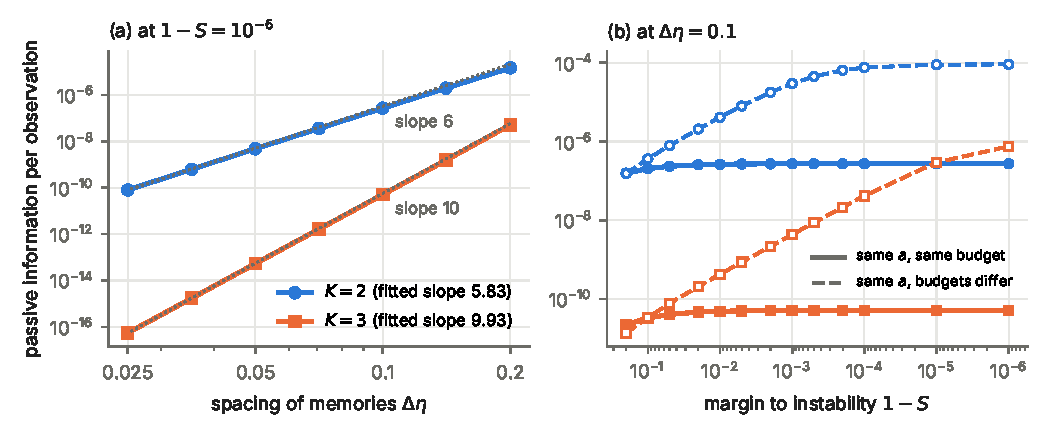
\includegraphics[width=\textwidth]{fig_barrier_admissible.pdf}
\caption{The passive barrier near instability. Both panels show the Gaussian Kullback--Leibler information per observation between the stationary price processes of two populations whose merged measures are the $K$-node Gauss and Gauss--Radau rules on memories spread over $\Delta\eta$ around $0.5$ (total weight $0.3$, impact $\kappa=0.5$). (a)~At a common persistence and a common feedback budget one millionth below instability, the information falls like $(\Delta\eta)^{4K-2}$ (dotted lines). (b)~With a common persistence and a common budget (solid; the Gauss--Radau weights rescaled by a factor $1+O((\Delta\eta)^{2K-1})$), the information stays bounded as the margin $1-S$ shrinks. With a common persistence and no rescaling (dashed), the budgets differ by order $(\Delta\eta)^{2K-1}$; the information then grows roughly like $(1-S)^{-1}$ until the margin reaches that gap, and levels off. Computed from the closed-form spectra.}
\label{fig:barrier}
\end{figure}


\section{Who needs composition, and what disclosure buys}\label{sec:supervision}

By Theorem~\ref{thm:eqinv}, composition is worth nothing to anyone trading on public information. It can still matter to a supervisor whose action is aimed at one group. This section gives a decision in which it does and the disclosure that removes the cost of learning it. It ends with a bound on what price-based targeting can achieve when a group can hide.

\paragraph{A decision in which attribution matters.} A supervisor must keep the feedback budget $S=a+\kappa\sum_iq_i$ below a prudential ceiling $\bar s$. It can either cut all activity uniformly or halt the largest verified class. The target is the feedback budget, not the spectral radius of the state matrix: in an already stable positive economy, imposing $S\le\bar s<1$ is a tighter prudential constraint, not a restoration of stability.


\begin{proposition}[Supervisory separation: market-wide versus targeted intervention]\label{prop:target}
Assume the positive stable model, known $a,\kappa$, and $a<\bar s<1$. Write $q_i=w_i/(1-r_i)$ and $R=S-\kappa\max_iq_i$ for the post-halt feedback budget.
\begin{enumerate}[label=(\roman*),itemsep=1pt]
\item A uniform scale $\theta$ meets the ceiling exactly when $a+\theta(S-a)\le\bar s$. Its largest feasible value is $\theta^*=\min\{1,(\bar s-a)/(S-a)\}$. The identity $S=1-\kappa/\sum_jh_j$ is algebraic; estimating this infinite sum requires a justified tail bound and an observation/noise model. It alone establishes no unconditional parametric learning rate.
\item For $K=2$, the Gauss and Gauss--Radau pair of Theorem~\ref{thm:kcohort} has limiting largest normalized weights $1/2$ and $3/4$. Thus $|S^G-S^R|=O((\Delta\eta)^3)$ and $q^R_{\max}-q^G_{\max}=W/(4(1-r_c))+O(\Delta\eta)$. For sufficiently small spacing, a nonempty interval of ceilings separates their post-halt decisions. For $N$ independent reset records with common Gaussian noise $\sigma^2 I$, both decision errors at most $1/4$ require
\[
 N\ge (2\Phi^{-1}(0.75)\sigma/\|h^G-h^R\|_2)^2
 \ge c\sigma^2(\Delta\eta)^{-6}.
\]
The record horizon and the response norm must be the same on both sides.
\item Tagged-flow estimation under Theorem~\ref{thm:discvalue}, a rate bound away from one, and a fixed nonzero decision margin gives a bounded sample requirement as the spacing shrinks. The target class must be mapped to an executable, verified class label; a largest latent atom alone supplies no such identity.
\end{enumerate}
\end{proposition}
The proof is in Supplement~\ref{app:decisionfull}. Proposition~\ref{prop:targetK} there extends part~(ii) to every $K$, with exponent $4K-2$.

\subsection{What class-tagged disclosure buys}


\begin{proposition}[Tagged flow removes the barrier]\label{prop:tagged}
Let the price $x_t$ be the causal stationary solution of the model driven by i.i.d.\ centered innovations of variance $\sigma_\xi^2\in(0,\infty)$ in a positive, stable economy, with stationary autocovariances $\gamma_x(s)=\sum_\ell c_\ell\lambda_\ell^{|s|}$ ($c_\ell\ge0$, $0\le\lambda_\ell<1$ the closed-loop modes). Suppose group $i$ has merged weight $w_i>0$ and the observer receives prices and each group's flow $\tilde u_{i,t}=u_{i,t}+\varepsilon_{i,t}$, $u_{i,t}=q_iy_{i,t}$, with i.i.d.\ centered measurement noise of finite variance $\sigma_f^2$, independent of the whole innovation sequence and hence of the whole price path. Then $\tilde u_{i,t}=r_i\tilde u_{i,t-1}+w_ix_t+e_{i,t}$ with $e_{i,t}=\varepsilon_{i,t}-r_i\varepsilon_{i,t-1}$, and the just-identified IV estimator of $\beta_i=(r_i,w_i)$ with instruments $Z_t=(x_{t-1},x_t)^\top$ satisfies $\sqrt T(\hat\beta_i-\beta_i)\to N(0,V_i)$,
\begin{equation}\label{eq:ivvar}
V_i=\Sigma_i^{-1}\Omega_i\Sigma_i^{-\top},\qquad \Sigma_i=\begin{pmatrix}w_iA_0&\gamma_x(1)\\ w_iA_1&\gamma_x(0)\end{pmatrix},\qquad \Omega_i=\sigma_f^2\bigl[(1+r_i^2)\Gamma_0-r_i(\Gamma_1+\Gamma_1^\top)\bigr],
\end{equation}
where $A_m=\sum_{s\ge0}r_i^s\gamma_x(s+m)$, $\Gamma_0=\begin{psmallmatrix}\gamma_x(0)&\gamma_x(1)\\ \gamma_x(1)&\gamma_x(0)\end{psmallmatrix}$ and $\Gamma_1=\E[Z_tZ_{t-1}^\top]$. The Jacobian determinant is
\begin{equation}\label{eq:ivdet}
\det\Sigma_i=w_i\sum_{\ell,m}c_\ell c_m\frac{1-\lambda_\ell\lambda_m}{1-r_i\lambda_m}\;>\;0 .
\end{equation}
$V_i$ depends only on group $i$'s own $(w_i,r_i)$, $\sigma_f^2$ and the price autocovariances. Two conclusions are distinct: (a) for each admissible economy, $\hat\beta_i$ has the stated limiting normal law; (b) on a uniformly stable family with stationary price variance at least $\gamma_{\min}>0$ and merged weights at least $w_{\min}>0$, the limiting covariance $V_i$ is bounded by a constant that does not depend on $|r_i-r_j|$. Statement (b) bounds the limit; it is not a central limit theorem that holds uniformly over the family.
\end{proposition}

\paragraph{Machine check.} Three pieces are machine-checked: the finite-sample reset-experiment version, with an error bound that does not depend on the spacing; the lower bound on the determinant of the population instrument matrix that does not depend on the spacing (\texttt{p1\_tagged\_iv\_determinant\_bound}); and the exact decomposition of the IV score into reporting-error terms with coefficients fixed by the price path plus two boundary terms (\texttt{p1\_iv\_boundary\_decomposition}). The stationary law of large numbers and the central limit theorem behind (a) are not machine-checked.


Each tagged flow follows $u_{i,t}=r_iu_{i,t-1}+w_ix_t$, a regression whose information about $w_i$ does not involve the other groups' rates; the closed form \eqref{eq:ivdet} matches the simulated Jacobian ($0.1330$ against $0.1322$ in a two-group economy with $4\times10^5$ periods). In simulation ($T=5{,}000$, 60 replications) the root-mean-square error of the recovered weights is flat in $\Delta\eta$ (fitted slope $0.011$, error between $5.8\times10^{-4}$ and $6.6\times10^{-4}$). This is the formal content of a disclosure regime such as a consolidated audit trail: tagging flow by participant class turns a polynomial barrier into an ordinary estimation problem.
Proposition~\ref{prop:tagged} says that tagging removes the barrier; the next result says by how much.

\begin{theorem}[Value of class-tagged disclosure]\label{thm:discvalue}
Take a rich class of Theorem~\ref{prop:esprit}: rates $r_c+\Delta\eta\,s$ with $s$ in a compact set of $\gamma$-separated ordered points that has nonempty interior and contains the Gauss and Gauss--Radau pair of Theorem~\ref{thm:kcohort}, and merged weights in a nondegenerate interval $[\omega_{\min},\omega_{\max}]$, $0<\omega_{\min}<\omega_{\max}$. In each reset experiment the observer applies a unit impulse and records the price response with independent $N(0,\sigma^2)$ noise per tap; under tagging it also records each class's flow response $f_{i,t}=w_i\sum_{s\le t}r_i^{\,t-s}h_s$ with independent $N(0,\sigma_f^2)$ noise per tap. Let $N_p$ and $N_t$ be the numbers of experiments needed, without and with tagging, for a fixed accuracy and confidence. There are constants $0<c\le C<\infty$, depending on $(\sigma,\sigma_f)$ and the class but not on $\Delta\eta$, such that
\begin{enumerate}[label=(\roman*),itemsep=1pt]
\item to recover the weights to a fixed accuracy smaller than half the weight difference between the Gauss and Gauss--Radau economies (so that recovering the weights decides between them), $c\le N_t\le C$, so $N_p/N_t\asymp(\Delta\eta)^{-(4K-2)}$;
\item to recover the rates to accuracy $c_0\Delta\eta$, for a fixed $c_0>0$ smaller than the radius of a ball contained in the class of rescaled nodes (so that no fixed guess meets the target), $c(\Delta\eta)^{-2}\le N_t\le C(\Delta\eta)^{-2}$, so $N_p/N_t\asymp(\Delta\eta)^{-(4K-4)}$.
\end{enumerate}
\end{theorem}

Proposition~\ref{prop:tagged} and Theorem~\ref{thm:discvalue} use different observation arrangements: the proposition concerns passive, stationary data with prices observed without noise, where the price is a valid instrument; the theorem concerns reset experiments with noisy prices. With noisy prices, regressing flow on the observed price is an errors-in-variables problem, which is why the theorem works from the known impulse instead.
\subsection{Partial disclosure}\label{sec:partial}

Actual regimes tag some traders and not others: Japan registers high-speed traders, India identifies algorithmic orders, and everyone else stays anonymous. Theorem~\ref{thm:discvalue} prices full tagging. The next result prices tagging some of the groups.

\begin{theorem}[Partial disclosure]\label{thm:partial}
In the reset experiments of Theorem~\ref{thm:discvalue}, let the flows of $m$ of the $K$ groups be recorded (tagged), and write $K'=K-m$ for the number of untagged groups.
\begin{enumerate}[label=(\roman*),itemsep=1pt]
\item \emph{Lower bound.} If $K'\ge2$, there are two $K$-group economies with rates in $r_c+\Delta\eta[-1,1]$ and positive weights, with identical tagged groups and with untagged groups forming the $K'$-node Gauss and Gauss--Radau pair of Theorem~\ref{thm:kcohort}, such that telling them apart from $N$ reset experiments, using the price records and the tagged flow records, with error probability below $1/4$ needs $N\ge c\,(\Delta\eta)^{-(4K'-2)}$.
\item \emph{Upper bound.} Let the tagged groups satisfy the conditions of Theorem~\ref{thm:discvalue}, and let the untagged groups range over a rich class of Theorem~\ref{prop:esprit} with $K'\ge2$ nodes. Estimate each tagged group from its flow records, subtract its contribution from the estimated kernel, and apply Prony's method with $K'$ nodes to the residual. This recovers the weights of all $K$ groups to any fixed accuracy from $N=C(\Delta\eta)^{-(4K'-2)}$ experiments.
\item \emph{One untagged group.} If $K'\le1$, the weights of all $K$ groups are recovered from a number of experiments that does not depend on $\Delta\eta$.
\end{enumerate}
The constants depend on $(\sigma,\sigma_f)$, the class and the tagged groups, not on $\Delta\eta$. So the cost of composition is that of the untagged groups alone: $N^*\asymp(\Delta\eta)^{-(4K'-2)}$ for $K'\ge2$.
\end{theorem}

\begin{proof}
(i) The two economies share the tagged groups, so their kernels differ only through the untagged pair, whose moments agree up to order $2K'-2$ (Theorem~\ref{thm:kcohort}); the kernel gap is therefore of order $(\Delta\eta)^{2K'-1}$ at every lag. The price impulse responses inherit this order through the closed-loop recursion, as in the proof of Theorem~\ref{thm:kcohort}, with constants that depend on the tagged groups only through the closed-loop stability margin. A tagged group's flow response, $f_{i,t}=w_i\sum_{s\le t}r_i^{\,t-s}h_s$, is the same linear map of the price response in both economies, so its mean difference is also of order $(\Delta\eta)^{2K'-1}$. With Gaussian noise the divergence of one experiment's full record is at most $C(\Delta\eta)^{4K'-2}$, and Le Cam's two-point lemma gives the bound.
(ii) As in the proof of Theorem~\ref{thm:discvalue}, the averaged price responses and least squares on each tagged class's flows estimate the tagged weights and rates with error $O_P(N^{-1/2})$, uniformly on the class and without dependence on $\Delta\eta$ or on the other groups. The kernel values $k_0,\ldots,k_{2K'-1}$ are smooth functions of the taps (proof of Theorem~\ref{prop:esprit}), so the residual kernel $k_j-\sum_{\rm tagged}\hat w_i\hat r_i^{\,j}$ estimates the untagged groups' kernel with error $O_P(N^{-1/2})$. Prony's method on these $2K'$ values is the estimator of Theorem~\ref{prop:esprit} with $K'$ nodes, whose error is the input error times order $(\Delta\eta)^{-(2K'-1)}$ (the rescaling of the centered moments). So the untagged weights have error $O_P(N^{-1/2}(\Delta\eta)^{-(2K'-1)})$, and $N=C(\Delta\eta)^{-(4K'-2)}$ suffices; the tagged weights are recovered at the faster rate.
(iii) With one untagged group of weight $v$ and rate $s$, $k_0=\sum_{\rm tagged}w_i+v$ and $k_1=\sum_{\rm tagged}w_ir_i+vs$, so $v$ and $s$ are smooth functions of $k_0$, $k_1$ and the tagged estimates, all estimated with error $O_P(N^{-1/2})$ independent of $\Delta\eta$. With none, this is Theorem~\ref{thm:discvalue}(i).
\end{proof}

\paragraph{Numerical check and machine check.} For $K=3$ with no tag and one tag, and $K=4$ with two tags, the exact divergence per experiment of the hard pair falls with $\Delta\eta$ at fitted slopes $10.05$, $6.02$ and $5.96$, against $10$, $6$ and $6$ (repository script \nolinkurl{reproduce.py}). Part~(i) is machine-checked on the joint records of prices and tagged flows, for records of any fixed length $T$ and a common noise variance $\sigma^2$ on prices and flows (with $\sigma_f\ne\sigma$, replace $\sigma$ by $\min(\sigma,\sigma_f)$): for any two economies that share their tagged groups and whose untagged node moments agree below order $n$, any test satisfies $4\sigma^2(1-\alpha_0-\beta_0)^2\le N(T+MT)\bigl(2W2^T(\Delta\eta)^nC_T(1+W_tT)\bigr)^2$ (\texttt{p1\_partial\_lower\_bound\_matched}, \nolinkurl{Paper1PartialDisclosureLower.lean}); with the matched $K'$-node pair of Theorem~\ref{thm:kcohort}, $n=2K'-1$. The algebraic steps of (ii) and (iii) are machine-checked too (\nolinkurl{Paper1PartialDisclosure.lean}), and so is the deterministic core of (ii): if the kernel taps are estimated within $e_k$ and the tagged weights and rates within $e_w$ and $e_r$, an ordered $K'$-node representation matching the residual moments exists, is unique and recovers every untagged weight within $L\,2^{2K'}\eta(\Delta\eta)^{-(2K'-1)}$, with $\eta=e_k+m(e_w+W_t\,2K'\,e_r)$ (\texttt{p1\_partial\_upper\_deterministic}, \nolinkurl{Paper1PartialDisclosureUpper.lean}). The $O_P(N^{-1/2})$ rates of the inputs are on paper, and the whole estimator is checked by Monte Carlo: subtract-then-Prony gives weight errors growing like $(\Delta\eta)^{-(2K'-1)}$, fitted slopes $-5.07$, $-3.02$ and $0.36$ for $K'=3,2,1$ untagged groups of three, against $-5$, $-3$ and $0$ (repository script \nolinkurl{reproduce.py}).

\subsection{Traders who respond to being watched}\label{sec:hiding}

The results so far take the groups' rules as given. A group that expects a targeted action has a reason to change its rule. Sufficiency bounds what a supervisor who relies on prices can then achieve.

\begin{proposition}[Hiding caps targeting]\label{prop:hiding}
A supervisor observes prices, under any probes and for a record of any length, and then targets a given group or not. Being targeted costs the group $P>0$. The group chooses among available rules. Rule $\rho$ has a private cost $C(\rho)\ge0$ and leads to targeting with probability $\pi(\rho)$. Suppose one available rule $\rho_0$, with cost $C_0$, gives the population the kernel of a population that the supervisor targets with probability $\alpha$.
\begin{enumerate}[label=(\roman*),itemsep=1pt]
\item $\pi(\rho_0)=\alpha$, whatever the supervisor's probes, record length and decision rule.
\item Every rule $\rho^*$ that minimizes the group's expected cost $C(\rho)+P\pi(\rho)$ satisfies
\[
\pi(\rho^*)\ \le\ \alpha+\frac{C_0-C(\rho^*)}{P}\ \le\ \alpha+\frac{C_0}{P}.
\]
\item Suppose the group has two rules: its original rule, with cost zero and targeting probability $\pi_T$ on a record of length $T$, and $\rho_0$. It adopts $\rho_0$ whenever $\pi_T>\alpha+C_0/P$. If $\pi_T\to1$ and $P(1-\alpha)>C_0$, this holds for all large $T$, and the targeting probability is then $\alpha$.
\end{enumerate}
\end{proposition}

\begin{proof}
(i) By Theorem~\ref{thm:eqinv}, populations with the same kernel give the same law of the price record for every probe sequence and every insider and dealer rule. The supervisor's decision is a function of that record and of its own randomization. (ii) $C(\rho^*)+P\pi(\rho^*)\le C_0+P\alpha$ by optimality, and $C(\rho^*)\ge0$. (iii) The original rule costs $P\pi_T$ and $\rho_0$ costs $C_0+P\alpha$.
\end{proof}


\section{Scope and limits}\label{sec:scope}

\paragraph{Linearity.} Sufficiency (Theorem~\ref{thm:eqinv}, Proposition~\ref{prop:anylinear}) needs aggregate feedback flow to be a linear function of past public signals, plus independent idiosyncratic shocks if there are any. With group-specific Gaussian demand shocks, a second aggregate enters, the spectral density of the aggregate shock process, and the equivalence class shrinks accordingly (Supplement~\ref{app:eqinv}). The passive results of Section~\ref{sec:cost} are stated for Gaussian innovations, the least favorable case: for any news law whose location divergence is quadratically bounded the passive orders are unchanged and the constant improves by the factor $\sigma^2I^*_f\ge1$ (\citealp[Proposition~S16.2]{niroula2026full}). Laws outside that class, such as news with bounded support, are not analyzed. Saturating rules are treated in \citet[Section~S6]{niroula2026full}. Other nonlinear rules, and traders who change their rules as they learn, are outside the theorems. \citet{niroula2026a} report simulations of stylized nonlinear rules and of online learners trained in the closed loop. In those simulations, the costs of Section~\ref{sec:cost} hold when the competing populations' feedback weights match. Populations whose learned weights differ are told apart by those weights instead. Hard thresholds hide groups from small probes altogether. These are simulations, not theorems.

\paragraph{Exponential memory.} The identification and cost results need memory to be a finite mixture of exponentials. For general completely monotone memory, \citet{niroula2026a} prove that the minimax accuracy for the memory distribution is of exact order $1/\log(N/\sigma^2)$. This is the severe ill-posedness of inverting a Laplace transform \citep{epstein2008}. Halving the error then squares the data needed, instead of multiplying it by a constant.

\paragraph{The observer.} The lower bounds hold for an observer who knows $(a,\kappa)$ and the noise law, so they hold a fortiori without that knowledge. The upper bound of Theorem~\ref{prop:esprit} also holds in one running market from an unknown state, with random-sign probes and news of any law with finite variance (\citealp[Theorem~S16.1]{niroula2026full}); the other upper bounds are stated for reset experiments. Strategic responses to being observed are modeled in Proposition~\ref{prop:hiding} and Supplement Section~\ref{app:dynamic} (traders who learn from prices, and a game of surveillance and hiding). Everywhere else the groups do not change their rules when probed.

\paragraph{Evidence.} \citet{niroula2026a} report pre-specified tests on two sets of trader-class reports: the CFTC's weekly Commitments of Traders in twenty futures markets and Binance's class ratios in 30 perpetual markets. Of 23 recorded outcomes, 11 pass. None is a direct test of a result in this paper: all use class positions or account ratios rather than executed flow tagged by class. The class reports constrain the persistence of class positions far more tightly than prices do. They do not identify learning memory, because that persistence can also reflect turnover, reporting aggregation or inventory retention. A pre-registered out-of-sample test of the feedback premise on Taiwan's tagged exchange flows (spec P1T, holdout 2019--2023; \citet{niroula2026a} report every diagnostic) gives the following. $D=0.0426$ $[0.0206, 0.0643]$, $p=0.000$, meets the registered supportive criterion. The pre-specified reverse-causality check gives $D=-0.0065$ $[-0.0316, 0.0165]$, which does not meet it. Under the registered rule that check is inconclusive rather than contrary: its interval contains both zero and the smallest effect of interest, and 68\% of stocks keep a positive gain after the adjustment (median $0.012$). By calendar year the primary gain meets the criterion in 2019--2021 and not in 2022--2023. The registered verdict is `supportive'. Read with its pre-specified diagnostic, the test does not provide evidence of feedback beyond prices revealing past flow. We do not claim that tagged flow in Taiwan responds to price deviations. The registered test is supportive, but its pre-specified diagnostic cannot separate the gain from prices revealing past flow.

A second test, of the two-layer prediction of \citet[Section~S6]{niroula2026full}, is registered on Binance perpetual futures (spec P7S, amendment A1). Its primary sample is retrospective (July 2024 to October 2026), specified in November 2026 after the sample period. The primary test was run once on 11 November 2026. A pre-specified test on Binance perpetual futures was inconclusive (calm difference $-0.002$, 90\% interval $[-0.007, 0.004]$; difference-in-differences $0.041$, $p=0.553$). It neither supports nor contradicts the prediction of \citet[Section~S6]{niroula2026full}.

\paragraph{Open problems.} The companion paper \citep{niroula2026c} answers several further questions: a long-lived insider cannot reveal or manipulate the groups' memory in a stable market, and a rational market maker nets feedback out (Companion Proposition~\ref{prop:insider}); a cascade after a breach has an exact threshold under mechanical impact (Companion Theorem~\ref{thm:cascade}); dead-band traders are identifiable by large probes (Companion Proposition~\ref{prop:deadband}). It also gives forward-looking dealers (several equilibria above the threshold; Companion Proposition~\ref{prop:reecascade}), saturation of every order (Companion Proposition~\ref{prop:smoothn}), a parametric rate for noisy stress identification with smooth shapes (Companion Proposition~\ref{prop:stressrate}) and the information content of learning traders (Companion Proposition~\ref{prop:learners}). It also covers a group that chooses its rule against an insider (Companion Proposition~\ref{prop:insidergame}), the path of a cascade, including slow-moving capital (Companion Proposition~\ref{prop:cascadedyn}), a parametric rate under hard limits (Companion Proposition~\ref{prop:hardrate}), the cost of composition when traders are nonlinear (Companion Proposition~\ref{prop:nlcost}), and the largest-weight comparison for every $K$ (Proposition~\ref{prop:maxweight}). What remains open: uniqueness of the insider game in cases where residual monotonicity fails (\citealp[Proposition~S17.3]{niroula2026full}); cascades whose dealers face richer constraints than a constant holding cost; hard-limit configurations whose kinks coincide; and upper bounds for nonlinear traders who share a leverage.




\subsection{Continuous double auctions, latency preemption, and frequent batch auctions}\label{sec:latency_batch}
In a continuous double auction (CDA) matching engine operating under price-time priority, incoming orders from algorithms with heterogeneous communication latencies $\ell_1 < \ell_2$ do not aggregate additively. When a trading signal arrives, a faster desk sweeps resting top-of-book depth $Q_{\mathrm{top}}$ before a slower Immediate-or-Cancel (IOC) order arrives, or cancels resting quotes (`zero-volume cancel race') ahead of marketable flow, making executed volume non-commutative: $\mathcal{M}(u_1, u_2; \ell_1, \ell_2) \neq \mathcal{M}(u_2, u_1; \ell_1, \ell_2)$. Continuous-book latency preemption and message cancellation thus break additive linear kernel aggregation unless paired with discrete call clearing or asymmetric resting-quote protection (such as speed bumps delaying aggressive takes relative to passive cancels, combined with MiFID~II RTS~9 convex order-to-trade ratio tariffs and minimum resting times that exempt bona fide passive quoting).

\begin{theorem}[Frequent batch auctions restore kernel sufficiency]\label{thm:batch_restoration}
Discretize trading into frequent uniform-price call auctions \citep{budish2015} over batch intervals $[T_{k-1}, T_k)$ with separate gross demand and supply schedules $D_k(p) = \bar{D}_k(p) + \sum_i u_{i,k}^+ \mathbf{1}_{\{p \le p^{\mathrm{cap}}_{i,k}\}}$ and $S_k(p) = \bar{S}_k(p) + \sum_i u_{i,k}^- \mathbf{1}_{\{p \ge p^{\mathrm{floor}}_{i,k}\}}$ ($u_{i,k} = u_{i,k}^+ - u_{i,k}^-$ against strictly monotone continuous exogenous limit schedules $\bar{S}_k - \bar{D}_k$), clearing price $p_k^* \in \arg\max_p \min(D_k(p), S_k(p))$, and marginal-only \citet{budish2015} uniform random tie-breaking (avoiding pro-rata order-padding incentives). Let batch durations follow either a deterministic baseline plus bounded uniform jitter $T_k - T_{k-1} = \tau + \tilde{\zeta}_k$ ($\tilde\zeta_k \sim U[0, \tau_{\mathrm{jitter}}]$) or an unbounded exponential clock $\mathrm{Exp}(\lambda)$. Then:
\begin{enumerate}
  \item[(i)] \emph{Arrival-order invariance and uncongested split linearity.} For any finite list of within-batch gross buy and sell submissions $\{(u_{i,k}^+, u_{i,k}^-)\}_{i=1}^K$ evaluated at clearing price $p_k^*$, two-sided cleared volume $V_k^* = \min(D_k(p_k^*), S_k(p_k^*))$ and uniform-fill individual executions are strictly invariant to microsecond arrival permutations and linear under order splitting at fixed fill ratio (reducing identically to submitted net flow $u_{i,k}$ on the uncongested branch).
  \item[(ii)] \emph{Uncongested kernel preservation and sniping bounds.} On the uncongested clearing branch with net flow invariance, any two trader populations matching power moments $\sum_{i=1}^K w_i r_i^m = \sum_{i=1}^K w'_i (r'_i)^m$ for $m < T$ generate pathwise identical batch net flows and pricing errors. Under an unbounded memoryless clock $\mathrm{Exp}(\lambda)$, boundary sniping probability is $1 - e^{-\lambda \Delta_{\mathrm{lat}}} \le \lambda \Delta_{\mathrm{lat}}$; under $\tau + U[0, \tau_{\mathrm{jitter}}]$ with $\Delta_{\mathrm{lat}} \le \tau$, unconditional arrival sniping is bounded by $\Delta_{\mathrm{lat}}/(\tau + \tau_{\mathrm{jitter}})$, whereas conditional on surviving into the closing jitter window $[\tau, \tau+\tau_{\mathrm{jitter}}]$, residual sniping share is $\min(1, \Delta_{\mathrm{lat}}/\tau_{\mathrm{jitter}})$.
\end{enumerate}
\end{theorem}
The deterministic call-auction, permutation-invariance, order-splitting, kernel-convolution, clearing-price monotonicity, and sniping-fraction claims are formalized in Lean~4 (\nolinkurl{PublicationRevision17.lean}, \nolinkurl{PublicationRevision18.lean}); stochastic clock distributions are proved on paper.

\section{Proofs of the main results}\label{app:proofs}

\noindent The proofs of main-text results other than Theorems~\ref{M-n:suff}, \ref{M-thm:what-id}, \ref{M-n:passiveupper}, \ref{M-n:separation} and~\ref{M-n:pilot}, which Main Appendix~\ref{M-app:proofs} proves, are given first.

\begin{proof}[Proof of Theorem~\ref{M-n:thm_inventory}]
\emph{(i)} Conjecture $x_t = -\kappa H_t + \sum_i \beta_i u_{i,t+1}$ and set $D = 1 - \sum_i \beta_i w_i$. Using $\E_t[\xi_{t+1}] = 0$, $\E_t[H_{t+1}] = \bar{a} H_t - \sum_i u_{i,t+1}$, and $\E_t[u_{i,t+2}] = r_i u_{i,t+1} + w_i \E_t[x_{t+1}]$, taking conditional expectations gives
\[
  D\, \E_t[x_{t+1}] = -\kappa \bar{a} H_t + \sum_i (\kappa + \beta_i r_i) u_{i,t+1}.
\]
The dealer optimality condition $x_t = \E_t[x_{t+1}] - A V H_t$ must hold identically in $(H_t, \{u_{i,t+1}\})$. Matching coefficients on $u_{i,t+1}$ yields $\beta_i = (\kappa + \beta_i r_i)/D$, so $\beta_i = \kappa / (D - r_i)$. Substituting into $D = 1 - \sum_i \beta_i w_i$ gives $D = 1 - \kappa S_M(D)$, and matching coefficients on $H_t$ gives $\kappa(D - \bar{a}) = A V D$. For the one-step innovation $\delta = x_{t+1} - \E_t[x_{t+1}]$, we have $\delta = \kappa \xi_{t+1} + \sum_i \beta_i w_i \delta$, hence $\delta = (\kappa/D)\xi_{t+1}$ and $V = \sigma_F^2 + \kappa^2 \sigma_\xi^2 / D^2$. Conversely, any stable solution of~main-text~\eqref{M-eq:eq-system} satisfies dealer optimality and variance consistency in every state.

\emph{(ii)} Setting $w_i = 0$ yields $S_M \equiv 0$, $D = 1$, $x_t = -\kappa H_t = \bar{a} x_{t-1} + \kappa Y_t$, and the quadratic $A \sigma_\xi^2 \kappa^2 - (1 - \bar{a})\kappa + A \sigma_F^2 = 0$, whose discriminant is $\Lambda_0 = (1 - \bar{a})^2 - 4 A^2 \sigma_F^2 \sigma_\xi^2$.

\emph{(iii)} The main-text system~\eqref{M-eq:eq-system} depends on the population solely through $S_M(D) = \int (D - r)^{-1} dM(r)$, hence solely through $M$.

\emph{(iv)} Define $\Phi(\kappa, D; M) = \bigl(D + \kappa S_M(D) - 1,\; \kappa(D - \bar{a}) - A(\sigma_F^2 D + \kappa^2 \sigma_\xi^2 / D)\bigr)$. At $M = 0$, $\Phi(\kappa_-, 1; 0) = 0$ with triangular Jacobian $\partial_D \Phi_1 = 1$, $\partial_\kappa \Phi_1 = 0$, and $\partial_\kappa \Phi_2 = (1 - \bar{a}) - 2 A \kappa_- \sigma_\xi^2 = \sqrt{\Lambda_0} > 0$. The implicit function theorem applied on the Banach space $C^1([1-\delta, 1+\delta])$ for $S_M$ yields a unique continuous branch near $(\kappa_-, 1)$ for small $\epsilon = \|S_M\|_{C^1}$. Linearizing gives $dD = -\kappa_- S_M(1)$ and $d\kappa = -\kappa_-(\bar{a} + 2 A \kappa_- \sigma_\xi^2)\, dD / \sqrt{\Lambda_0}$, with $S_M(1) = \sum_i w_i/(1 - r_i) = \sum_i q_i$. Stability holds by continuity of eigenvalues from $M = 0$.
\end{proof}

\begin{proof}[Proof of Theorem~\ref{M-thm:fragility}]
Substituting $V = \sigma_F^2 + \kappa^2 \sigma_\xi^2 / D^2$ into $\kappa(D - \bar{a}) = A V D$ yields $A \sigma_\xi^2 \kappa^2 - D(D - \bar{a})\kappa + A \sigma_F^2 D^2 = 0$, whose discriminant $\Lambda(D) = D^2[(D - \bar{a})^2 - 4 A^2 \sigma_F^2 \sigma_\xi^2]$ is positive iff $D > D_{\min}$. On $(D_{\min}, 1]$, both quadratic roots $\kappa_\pm(D) = [D(D - \bar{a}) \pm \sqrt{\Lambda(D)}]/(2 A \sigma_\xi^2)$ are strictly positive with $\kappa_+(D) > \kappa_-(D)$ and $\kappa_-(1) = \kappa_-$. For $D \in (\max(D_{\min}, \max_i r_i), 1]$ with $w_i > 0$, $S_M(D) > 0$ and is strictly decreasing in $D$, while $\kappa_-(D)$ decreases on $(D_{\min}, 1]$ and $d\kappa_-/dD \to -\infty$ as $D \downarrow D_{\min}$ (and $S_M(D) \to +\infty$ as $D \downarrow \max_i r_i$). Setting $F_\pm(D; \lambda) \equiv D - 1 + \lambda \kappa_\pm(D) S_M(D)$, we have $F_-(1; \lambda) = \lambda \kappa_- S_M(1) > 0$, $F_-(D; 0) = D - 1 < 0$ for $D < 1$, and $F_-(D; \lambda) \to +\infty$ as $D \downarrow D_* \equiv \max(D_{\min}, \max_i r_i)$. Thus $\lambda_{\mathrm{crit}} = \sup_{D \in (D_*, 1)} (1 - D)/[\kappa_-(D) S_M(D)] > 0$ is attained at an interior point $D_{\mathrm{crit}} \in (D_*, 1)$; because both $\kappa_-(D)$ and $S_M(D)$ strictly decrease on $(D_*, 1]$ and $1 - D_{\mathrm{crit}} < 1$, $\kappa_-(D_{\mathrm{crit}}) S_M(D_{\mathrm{crit}}) > \kappa_- S_M(1)$, proving strictly $\lambda_{\mathrm{crit}} < [\kappa_- S_M(1)]^{-1}$, with $F_+(D;\lambda) > F_-(D;\lambda) > 0$ for all $\lambda > \lambda_{\mathrm{crit}}$ so neither root exists on $(D_*, 1]$. At the interior fold $D_{\mathrm{crit}} > D_*$, $\Lambda(D_{\mathrm{crit}}) > 0$. By Vieta's identity on the quadratic $A \sigma_\xi^2 \kappa^2 - D(D-\bar{a})\kappa + A \sigma_F^2 D^2 = 0$, the two roots satisfy $\kappa_-(D) < \kappa_+(D)$ and $\kappa_+(D)\kappa_-(D) = (\sigma_F^2/\sigma_\xi^2) D^2$, so $[\kappa_-(D)/D]^2 \sigma_\xi^2 < \kappa_+(D)\kappa_-(D)\sigma_\xi^2/D^2 = \sigma_F^2$ and hence $V(\lambda_{\mathrm{crit}}) = \sigma_F^2 + (\kappa_{\mathrm{crit}}/D_{\mathrm{crit}})^2 \sigma_\xi^2 < 2\sigma_F^2 < \infty$. Also by Theorem~\ref{M-n:thm_eqreduced}(i), $S^*(\lambda_{\mathrm{crit}}) = 1 - \frac{D_{\mathrm{crit}}-\bar{a}}{D_{\mathrm{crit}}}\frac{S_M(1)}{S_M(D_{\mathrm{crit}})} < 1$ because $D_{\mathrm{crit}} > \bar{a}$ and $S_M(D_{\mathrm{crit}}) > S_M(1) > 0$, keeping $\Var(H_t) < \infty$. At the non-degenerate fold ($F_D = 0, F_{DD} > 0, F_\lambda > 0$), expanding $F_-(D; \lambda) \approx \frac{1}{2} F_{DD}(D - D_{\mathrm{crit}})^2 + F_\lambda(\lambda - \lambda_{\mathrm{crit}})$ yields $D - D_{\mathrm{crit}} \asymp \sqrt{\lambda_{\mathrm{crit}} - \lambda}$ and $d\kappa/d\lambda, dV/d\lambda, d\Var(H_t)/d\lambda \asymp (\lambda_{\mathrm{crit}} - \lambda)^{-1/2} \to +\infty$.
\end{proof}

\begin{proof}[Proof of Theorem~\ref{M-n:thm_eqreduced}]
\emph{(i)} Write $D x_t = -\kappa H_t + \sum_i \beta_i r_i u_{i,t}$ and $x_{t-1} = -\kappa H_{t-1} + \sum_i \beta_i u_{i,t}$, where $\beta_i = \kappa/(D - r_i)$. Substituting $H_t = \bar{a} H_{t-1} - \sum_i u_{i,t} - \xi_t$ yields
\[
  D x_t - \bar{a} x_{t-1} = \kappa \xi_t + \sum_i \bigl(\kappa + \beta_i(r_i - \bar{a})\bigr) u_{i,t} = \kappa \xi_t + \sum_i \kappa \frac{D - \bar{a}}{D - r_i}\, u_{i,t}.
\]
Dividing by $D$ and defining $\tilde{u}_{i,t} = \frac{D - \bar{a}}{D - r_i} u_{i,t}$ gives $x_t = a^* x_{t-1} + \kappa^*(\xi_t + \sum_i \tilde{u}_{i,t})$ and $\tilde{u}_{i,t+1} = r_i \tilde{u}_{i,t} + \tilde{w}_i x_t$ pathwise, with $(a^*, \kappa^*, \tilde{w}_i)$ as stated. Because $\kappa \neq 0$ and $D \neq \bar{a}$, the state transformation is invertible and preserves stability.

\emph{(ii)}-- \emph{(iii)} Part~(ii) follows from Theorem~\ref{thm:minphase}(i) applied to the closed loop in~(i). For~(iii), $S_M(D) = \sum_i \tilde{w}_i/(D - \bar{a})$ turns $D = 1 - \kappa S_M(D)$ into $D = 1 - \kappa^* \tilde{M}([0,1])/(1 - a^*)$, which recovers $D$, $\bar{a} = a^* D$, $\kappa = \kappa^* D$, and $M = h^{-1} \tilde{M}$ uniquely.

\emph{(iv)} Given any hard pair $(a^*, \kappa^*, W, r_c, \Delta\eta)$ satisfying the stability condition $a^* + \kappa^* W / (1 - r_c - \Delta\eta) < 1$, we have $\kappa^* W / (1 - a^*) < 1 - r_c - \Delta\eta$, so setting $D = 1 - \kappa^* W/(1 - a^*)$ ensures $D > r_c + \Delta\eta \ge \max_i r_i$. Choosing $\bar{a} = a^* D$, $\kappa = \kappa^* D$, any $\sigma_F^2, \sigma_\xi^2 > 0$, $A = \kappa^* D(1 - a^*)/(\sigma_F^2 + \kappa^{*2} \sigma_\xi^2)$, and $w_i = \tilde{w}_i(D - r_i)/(D - \bar{a}) > 0$ realizes both economies as equilibria with identical primitives $(A, \sigma_F^2, \sigma_\xi^2, \bar{a})$ and identical $(\kappa, D)$, preserving the $(\Delta\eta)^{-(4K-2)}$ lower bound.
\end{proof}

\begin{proof}[Proof of Theorem~\ref{M-n:cost}]
Let $n=2K-1$ and normalize the $K$-node Gauss--Legendre and left Gauss--Radau rules to mass one. Both integrate degree $n-1$ exactly. Their degree-$n$ moments differ because the monic polynomial $(s+1)\prod_{j>1}(s-s_j)^2$ vanishes at all Radau nodes and has positive integral, which the Gauss rule integrates exactly. Scale the nodes by $r_c+\Delta\eta s$ and masses by $W$. Taylor expansion gives $|\Delta k_m|\le 2W\binom{m}{n}(\Delta\eta)^n(r_c+\Delta\eta)^{m-n}$ for $m\ge n$, with zero difference before that and $|\Delta k_n|\asymp(\Delta\eta)^n$. In particular $\|\Delta k\|_1=O((\Delta\eta)^n)$ uniformly.

Write the innovation filter as $B_X(z)=[1-az-\kappa z\sum_{m\ge0}k_{X,m}z^m]^{-1}$ in the lag variable and the reset response as $h_X=\kappa B_X$. The uniform stability bound gives bounded $\ell^1$ norms of the filters by the geometric series for the inverse. Subtracting the inverse filters shows $\|h_1-h_0\|_2\le C\|\Delta k\|_1$; the first nonzero difference is $\kappa^2\Delta k_n$ at lag $n+1$. The reset KL is $N\|h_1-h_0\|_2^2/(2\sigma^2)$ for the observed taps. Both errors at most $1/4$ imply TV at least $1/2$ and KL at least $1/2$ by Pinsker.

For stationary prices the spectral ratio is $f_1/f_0=|B_1/B_0|^2=1+O((\Delta\eta)^n)$ uniformly, with spectra bounded above and away from zero. The leading ratio term is twice the real part of a nonzero analytic function on the disk which vanishes at zero: use the resolvent identity and the leading Taylor term of $\sum_m \Delta k_m z^m$, whose coefficient at $z^n$ is nonzero. Its real part cannot vanish identically on the unit circle: it is harmonic on the disk, so it would then vanish on the whole disk by the maximum and minimum principles for harmonic functions, making the function an imaginary constant, which is zero because the function vanishes at zero. The integral of its square over the circle is therefore positive. Thus the Gaussian spectral integral of $(f_1/f_0)-1-\log(f_1/f_0)$ has exact order $(\Delta\eta)^{2n}$. For finite records the uniform ratio bound sandwiches the two Toeplitz covariance matrices, putting the eigenvalues of their relative covariance within $O((\Delta\eta)^n)$ of one. Summing the quadratic bound on $\lambda-1-\log\lambda$ gives KL $\le CT(\Delta\eta)^{2n}$, so the same testing argument applies.

For recovery, the impulse recursion inverts the first $2K$ kernel taps triangularly, with nonzero divisor $\kappa h_0=\kappa^2$. Averaging independent Gaussian responses gives tap errors $O_P(\sigma/\sqrt N)$ at fixed depth. Centering the kernel moments at $r_c$ and dividing moment $j$ by $(\Delta\eta)^j$ gives errors $O_P(\sigma/(\sqrt N(\Delta\eta)^n))$. On the separated class the ordered rescaled moment map is injective by the Vandermonde equations for the difference of two atomic measures. Its Jacobian is a nonsingular confluent Vandermonde with weights bounded away from zero. The inverse function theorem and compactness give a uniformly Lipschitz local inverse. On its domain the Prony reconstruction returns that inverse, giving the stated fixed-accuracy rate.
\end{proof}

\begin{proof}[Proof of Theorem~\ref{M-n:questions}]
The largest difference of $F_g$ between two positive measures of mass at most $\bar W$ with tap distance at most $\delta$ is the displayed modulus. To see this, enforce the norm constraint by infimizing $\delta\|c\|_2-c\cdot(k_1-k_0)$ over $c$. Exchange infimum and supremum by convex minimax on the weak-star compact pair of measure sets. The residual supremum is $\bar W\mathcal R(g-p_c)$, with $p_c(r)=\sum_{t<L}c_t r^t$. Two Gaussian means at tap distance below $2z_{1-\alpha}\sigma/\sqrt N$ have TV below $1-2\alpha$, so uniform coverage forces answer separation at most $2\epsilon$. Continuity of the modulus gives the boundary. For sufficiency center the residual range and use the affine tap estimate. Its worst-case bias is at most $\bar W\mathcal R(g-p_c)/2$ and its standard deviation is $\sigma\|c\|_2/\sqrt N$.

If the coefficients of $g$ belong to $\ell^2$, truncation gives uniform residual $O(\bar r^L)$ by Cauchy--Schwarz. Choose logarithmic depth to make it $O(\epsilon)$ with bounded coefficient norm. Conversely the necessary condition with $N=O(\sigma^2\epsilon^{-2})$ gives polynomial approximants with bounded coefficient norms and residual tending to zero. Pad their coefficients with zeros and extract a weakly convergent subsequence in $\ell^2$. Point evaluation on $[0,\bar r]$ is continuous on coefficient space, so the limit represents $g$. For (iii) compare zero mass with $c\delta_r$ where $c=d\sigma\sqrt{(1-r^2)/N}$, with $0<d<1-2\alpha$ and $d$ small enough that $c\le\bar W$. Even with all taps observed, the divergence of the averaged record is $N\sum_m c^2r^{2m}/(2\sigma^2)=d^2/2$, so by Pinsker's inequality the total variation is at most $d/2<1-2\alpha$, yet the answer separation $c\,|g(r)|$ is unbounded as $r\uparrow1$. This contradicts uniform coverage.
\end{proof}


\begin{proof}[Proof of Proposition~\ref{M-n:target}(i)--(ii) and Corollary~\ref{M-n:decisionloss}]
Uniform scaling multiplies the feedback part of $S$ by $\theta$. For the halt, take the quadrature rules at the zeros of $p_K-cp_{K-1}$, where $p_j$ are orthonormal for the uniform probability on $[-1,1]$. For small $c$ the zeros stay simple and interior. The interpolatory rule integrates degree $2K-2$ exactly: divide by $p_K-cp_{K-1}$ and use orthogonality of the quotient of degree at most $K-2$. Products of the Lagrange polynomials show that their squared norms are the weights. Normalizing them to an orthonormal basis gives weight $1/\sum_{j<K}p_j(s)^2$ at a node $s$. As $c$ varies, a node cannot recur, since consecutive orthogonal polynomials have no common zero by the three-term recurrence. Each weight level set is finite, so two such rules have distinct largest weights. After shifting and scaling, Taylor expansion of $(1-r)^{-1}$ gives an $O((\Delta\eta)^{2K-1})$ difference in total feedback. The largest activities converge to the different largest masses divided by $1-r_c$, giving separated post-halt budgets for small spacing. The reset KL proof above applies to this moment-matched pair.

For the binary decision let $A$ be the event of choosing the halt. Its excess loss is $(bP_0(A)+cP_1(A^c))/2\ge \min(b,c)(1-\TV)/2$. Apply Pinsker and solve for the required length. For equal-covariance Gaussian records the equal-prior likelihood rule has each error $\Phi(-\sqrt{N}\|d\|/(2\tau))$; the normal tail bound gives the displayed risk bound.
\end{proof}

\begin{proof}[Proof of Proposition~\ref{M-n:target}(iii)]
Let $x_K < 1$ be the largest node of the $K$-point Gauss--Legendre rule on $[-1, 1]$, and place the hard pair of Theorem~\ref{M-n:cost}, with a common persistence and total merged weight $W$, on $r_c + \Delta\eta[-1, 1]$ with $r_c = \hat r + (1 + x_K)\Delta\eta/2$. Its memories lie in $[\hat r - \Delta\eta, \hat r + 2\Delta\eta]$. The Gauss--Radau economy has an atom of weight $W/K^2$ at $r_c - \Delta\eta < \hat r$, because the endpoint weight of the $K$-point Gauss--Radau rule on $[-1, 1]$ is $2/K^2$. Every memory of the Gauss economy is at least $r_c - x_K\Delta\eta > \hat r$. Group $i$ contributes $\kappa q_i = \kappa w_i/(1 - r_i)$ to the budget, so the restriction removes at least $\kappa W/K^2$ in the Gauss--Radau economy and nothing in the Gauss economy. The budgets themselves, $a + \kappa\int (1 - r)^{-1}\,dM(r)$, differ by $O((\Delta\eta)^{2K-1})$, because the merged measures match moments $0, \dots, 2K-2$ and $(1 - r)^{-1}$ is smooth near $r_c$. For small $\Delta\eta$ the budgets after the restriction therefore differ by at least $\kappa W/(2K^2)$, and every ceiling between them is met in one economy and breached in the other. The record length is that of Theorem~\ref{M-n:cost}(ii), which concerns the same pair.
\end{proof}

\begin{proof}[Proof of Proposition~\ref{prop:instrument_bound}]
Concavity gives $q=\min\{c/T_h,(\beta A_hV-\tau T_h)_+/(bV+\nu D_h/h)\}$. At revision dates the conditional perceived payoff and the quadratic risk cost scale with $V$, while Gaussian changes give expected absolute volume $qT_h$ per date. A constant signal produces constant $y$, so the ratio of scales gives the stated budget formula after aggregation.

Write $\gamma_j=\E[x_t x_{t-j}]$, $B(z)=\sum_{j\in\mathbb Z}\gamma_j z^{|j|}$,
$B_h(z)=\sum_{j\in\mathbb Z}\gamma_{j+h} z^{|j|}$, and $C_h(z)=2(B(z)-B_h(z))/(1-z)$. Summing by the difference of the filter indices gives $V=(1-r)B(r)/(1+r)$ and $D_h/V=(1-r)C_h(r)/B(r)$. The geometric bound extends the series past the unit circle. Since $B(1)=B_h(1)$, $C_h$ extends there too. The real part of $B$ is uniformly positive on the circle by the spectral bound, and hence in the disk. For the quadratic charge from zero,
\[
 g=\frac{\nu C_1}{bB+\nu(1-r)C_1}.
\]
For scheduled revisions, division by the old scale gives
\[
 g=\frac{1-A_h}{1-r}+
 \frac{A_h\nu(C_h/h-C_1)}{bB+\nu(1-r)C_h/h}.
\]
Small $\nu$ keeps both denominators bounded away from zero throughout the disk. The analytic terms have uniformly bounded square-summable Taylor coefficients. For a white-noise reference with variance $\gamma_0$, $T_1/V=2\sqrt{(1+r)/(\pi\gamma_0)}$. Thus $d=2\tau/(\beta\sqrt{\pi\gamma_0})$ in (a). The analytic continuation from an active interval grows like $(1-r)^{-1}$, whereas a square-summable Taylor series is bounded by its coefficient norm times $(1-r^2)^{-1/2}$. The same argument applies to the first term in (b) when $A_h<1$.

For the plug-in estimate, Wick's formula bounds the variance of each sample covariance up to lag $\lfloor n/2\rfloor$ by $C/n$. Summing errors with geometrically decaying weights on $[0,\bar r]$ gives uniform error $O_P(n^{-1/2})$ for the analytic term, after flooring denominators. Fit a degree-$<L$ polynomial to it in uniform norm with a known coefficient-norm bound. The truncated true series is feasible with error $O(\bar r^L)$. The resulting integrated bias is bounded by total mass times $O_P(n^{-1/2}+\bar r^L)$. Given the independent reference record, the tap statistic's variance is $O(\sigma^2/N)$ by the norm bound. Take logarithmic depth to make the tail no larger than the sampling errors.


In the passive alternative write $J(z)=\kappa\sum_{m\ge0}k_mz^m$ and $Q(z)=1-z(a+J(z))$. The memory and stability margins bound $Q$ away from zero on a disk larger than the unit disk and yield uniform geometric covariance decay. The stationary spectrum is $f=\sigma^2/|Q|^2$ in the covariance-series normalization. With $\ell_j$ the positive Fourier coefficients of $\log f$ under $z=e^{-i\omega}$ and $Q(0)=1$,
\[
 Q(z)=\exp\{-\textstyle\sum_{j\ge1}\ell_j z^j\},\qquad J(z)=(1-Q(z))/z-a .
\]
The constant coefficient absorbs the variance scale. A covariance series estimated to logarithmic lag depth has uniform error $O_P(\log n/\sqrt n)$, so linearizing its log leaves an $o_P(n^{-1/2})$ remainder. Each linear Fourier coefficient is a Gaussian quadratic form whose squared matrix Frobenius norm is bounded by $C/n$ times the squared sum of its Fourier weights. Parseval bounds the weights of $e^{ij\omega}/f$ uniformly in $j$. Geometric summation on any interior circle gives $\|\hat J-J\|_s=O_P(n^{-1/2})$.

Estimate $g$ from the same sample covariances. The analytic terms extend uniformly to a disk larger than the unit disk, so their coefficients have a uniform weighted sum bound $\sum_m R^m|c_m|\le B$ for some $R>1$. Fit the pilot at logarithmic depth under that bound. Its fitted polynomial approximates $g$ on the memory interval with $O_P(n^{-1/2})$ error by the preceding approximation argument. Choose $R^{-1}<s<1$. Cauchy's integral estimate gives $|\sum_m\hat c_m(\hat J_m-J_m)|\le B\|\hat J-J\|_s$. Integrating the weight error costs at most $\kappa M([0,\bar r])\|\hat g-g\|_\infty$. These pathwise bounds allow both fits to use the same observations. Section~\ref{app:passiveincidence} gives details.

At an interior transversal exit or binding point $r_*$, the positive part gives a nonzero jump $\Delta g'$ of the one-sided derivative of $g$. Locally $g(r)=g(r_*)+g'_-(r-r_*)+\Delta g'(r-r_*)_++O((r-r_*)^2)$. Reflect the Gauss--Legendre and left Gauss--Radau pair of Theorem~\ref{M-n:cost} and place it so that only the Radau endpoint lies on the clipped side, at distance $u\Delta\eta$ for a fixed $u>0$. A reflection of the construction for Proposition~\ref{M-n:target}(iii) gives the opposite orientation if needed. The affine terms cancel, and the lone endpoint generates a nonzero term of magnitude $|\Delta g'|Wu\Delta\eta/K^2$. The quadratic remainder is $O((\Delta\eta)^2)$. The common reference record carries no additional information about the pair. The reset KL is $O(N(\Delta\eta)^{4K-2}/\sigma^2)$ from moment cancellation. Applying the same two-point test to the binary decision or to estimates with disjoint accuracy intervals proves the bounds. For caps, the policy scale is $\min(q^0,c/T_1)$ and the same derivative jump follows at a transversal binding point.
\end{proof}

\begin{proof}[Proof of Theorems~\ref{M-n:minimax} and~\ref{n:minimaxtags} and Corollary~\ref{cor:robustuniform}]
For Theorem~\ref{M-n:minimax}, averaging over all $K!$ permutations $\pi \in S_K$ places every label on every class equally often:
\[
  \frac{1}{K!} \sum_{\pi \in S_K} S'_\pi = a + \sum_{c=1}^K \theta_c \Bigl(\frac{1}{K} \sum_{d=1}^K u_d\Bigr) = a + \bar{\theta} U,
  \qquad
  \frac{1}{K!} \sum_{\pi \in S_K} \theta \circ \pi = \bar{\theta}\mathbf{1}.
\]
By convexity of $\ell$ and $C$ (and permutation invariance of $C$), Jensen's inequality gives part~(i):
\[
  \ell(a + \bar{\theta} U) + C(\bar{\theta}\mathbf{1})
  \le \frac{1}{K!} \sum_{\pi} \ell(S'_\pi) + C(\theta)
  \le \max_{\pi} \ell(S'_\pi) + C(\theta).
\]
For part~(ii), suppose $\theta \in [0, 1]^K$ is non-uniform, so $\theta_{c_1} \neq \theta_{c_2}$ for some $c_1 \neq c_2$. Then the transposition $\tau = (c_1\, c_2)$ satisfies $\theta \circ \tau \neq \theta$. Since $\bar{\theta}\mathbf{1} = \frac{1}{K!}\sum_{\pi \in S_K} (\theta \circ \pi)$ is a strictly positive convex combination of points that are not all equal, strict convexity and permutation invariance of $C$ yield $C(\bar{\theta}\mathbf{1}) < \frac{1}{K!}\sum_\pi C(\theta \circ \pi) = C(\theta)$, giving strict dominance. (Similarly, if $u_{d_1} \neq u_{d_2}$ and $\theta_{c_1} \neq \theta_{c_2}$, swapping the assignment of $d_1, d_2$ to $c_1, c_2$ produces distinct budgets $S'_{\pi_1} \neq S'_{\pi_2}$, so strict convexity of $\ell$ yields $\ell(a + \bar{\theta} U) < \frac{1}{K!}\sum_\pi \ell(S'_\pi) \le \max_\pi \ell(S'_\pi)$.) Hence every minimax-optimal policy must be uniform; on the compact interval $[0, 1]$, the strictly convex continuous function $\bar{\theta} \mapsto \ell(a + \bar{\theta} U) + C(\bar{\theta}\mathbf{1})$ attains a unique minimizer $\bar{\theta}^*$. Thus $\bar{\theta}^*\mathbf{1}$ is the unique minimax supervisory policy.
For Corollary~\ref{cor:robustuniform}, halting label $c$ leaves budget $S - u_{\pi(c)}$, whose worst case over $\pi$ is $S - \min_d u_d$, attained whenever $\pi(c) \in \arg\min_d u_d$. A uniform cut $\theta = (\bar{s} - a)/(S - a)$ yields budget $a + \theta(S - a) = \bar{s}$ exactly and removes total feedback $(1 - \theta)(S - a) = S - \bar{s}$, the algebraic minimum needed to reach $\bar{s}$. For Theorem~\ref{n:minimaxtags}, restrict the averaging group to the product of within-group permutations $\prod_{g=1}^G S_g$: within each group $g$, every label averages to $\bar{\theta}_g$, so the averaged budget is $a + \sum_g \bar{\theta}_g U_g$ and the identical Jensen argument yields the minimax bound and $V_{\mathrm{tag}} \ge 0$.
\end{proof}

\begin{proof}[Proof of Theorem~\ref{M-n:disc}]
The first two noiseless class-flow coordinates are $w_i h_0$ and $w_i(h_1+r_i h_0)$. Since $h_0=\kappa>0$ and $w_i$ is bounded below, sample averages of these and of the price taps estimate both parameters with error $O_P(N^{-1/2})$ uniformly, using ratios on an event where denominators stay bounded away from zero. This suffices for fixed weight accuracy and for the specified shrinking rate accuracy. In an interior ball choose two rate vectors separated by more than twice the target, with identical weights. Their physical rates differ by $O(\Delta\eta)$, and the finite observed means differ by $O(\Delta\eta)$ by smoothness. Thus the Gaussian two-point bound requires order $(\Delta\eta)^{-2}$ tagged experiments. The untagged weight comparison follows from Theorem~\ref{M-n:cost}.
\end{proof}

\begin{proof}[Proof of Lemma~\ref{M-lem:micro}]
\emph{(i)} Linearizing social welfare around the no-feedback equilibrium of Theorem~\ref{M-n:thm_inventory}(iv), each retained unit of class $j$ yields private surplus $b_j$ and raises aggregate feedback intensity by $\phi_j$, increasing equilibrium impact $\kappa$ proportionally to $\kappa_-^2(\bar{a} + 2A\kappa_-\sigma_\xi^2)/\sqrt{\Lambda_0} > 0$. Valuing a unit of feedback intensity at $\lambda_{\mathrm{ext}} > 0$, the supervisor's valuation of the rise in impact and inventory risk, gives the first-order net social value $n_j = b_j - \lambda_{\mathrm{ext}}\phi_j$, with $n_{\mathcal{H}} < 0 < n_{\mathcal{B}}$ under the stated sign conditions.

\emph{(ii)} Under $\hat{v}_{t+1} = r \hat{v}_t + (1 - r)(v_t + \nu_t)$, the forecast error $e_t = v_t - \hat{v}_t$ evolves as $e_{t+1} = r e_t + \zeta_{t+1} - (1 - r)\nu_t$. Taking stationary variances with independent innovations gives $P(r) = r^2 P(r) + \sigma_\zeta^2 + (1 - r)^2 \sigma_\nu^2$, so
\[
  P(r) = \frac{\sigma_\zeta^2 + (1 - r)^2 \sigma_\nu^2}{1 - r^2}
       = \frac{\sigma_\zeta^2}{1 - r^2} + \frac{2\sigma_\nu^2}{1 + r} - \sigma_\nu^2,
\]
using $(1 - r)^2 / (1 - r^2) = (1 - r)/(1 + r) = 2/(1 + r) - 1$. Differentiating twice on $(0, 1)$ gives
\[
  P'(r) = \frac{2 r \sigma_\zeta^2}{(1 - r^2)^2} - \frac{2\sigma_\nu^2}{(1 + r)^2},
  \qquad
  P''(r) = \frac{2\sigma_\zeta^2(1 + 3r^2)}{(1 - r^2)^3} + \frac{4\sigma_\nu^2}{(1 + r)^3} > 0.
\]
Since $P'(0) = -2\sigma_\nu^2 < 0$, $\lim_{r \uparrow 1} P'(r) = +\infty$, and $P''(r) > 0$ throughout $(0, 1)$, $P$ is strictly convex with a unique interior minimizer $r_0 \in (0, 1)$ satisfying $P'(r_0) = 0$. Substituting the plug-in trade at the same date and fixed impact $u_t = \hat{v}_t / (\kappa + \lambda)$ into expected profit gives $\Pi(r) = \frac{1}{2(\kappa + \lambda)}\bigl(\E[v_t^2] - P(r)\bigr)$ (since $\E[v_t \hat{v}_t] - \frac{1}{2}\E[\hat{v}_t^2] = \frac{1}{2}\E[v_t^2] - \frac{1}{2}\E[(v_t - \hat{v}_t)^2]$), so
\[
  \Pi(r_0) - \Pi(r) = \frac{P(r) - P(r_0)}{2(\kappa + \lambda)}
  = \frac{P''(r_0)}{4(\kappa + \lambda)}(r - r_0)^2 + O\!\left(|r - r_0|^3\right).
\]
The term $\E[v_t^2]$ may grow with calendar time but cancels when the two rules are compared at the same date.
\end{proof}

\begin{proof}[Proof of Theorem~\ref{M-n:recordvalue}]
\emph{(i)} Let $p_0, p_1$ be densities of $P_0, P_1$ with respect to $P_0 + P_1$, let $a = \min(p_0, p_1)$, and let $\theta(x)$ be the policy. Since $\tfrac12\{W(\theta, 0) + W(\theta, 1)\} \le W_\varnothing$ for every $\theta$, $\int a = 1 - \TV(P_0, P_1)$ and $\int (p_0 - a) = \int (p_1 - a) = \TV(P_0, P_1)$,
\begin{align*}
  \mathbb{E}\, W &= \int a\, \tfrac12\{W(\theta(x), 0) + W(\theta(x), 1)\} \\
  &\quad + \tfrac12 \int (p_0 - a) W(\theta(x), 0) + \tfrac12 \int (p_1 - a) W(\theta(x), 1) \\
  &\le (1 - \TV) W_\varnothing + \TV\, \tfrac12\{\max_\theta W(\theta, 0) + \max_\theta W(\theta, 1)\}.
\end{align*}
Subtracting $W_\varnothing$ gives the first bound, and Pinsker's inequality the second. \emph{(ii)} By Theorem~\ref{M-n:paradox}(ii), $(\delta^*)^{n-2} \le B_N$ for every $N$, so $J^* = cN(\delta^*)^n \le cN B_N^{n/(n-2)}$; at $n = 4$ this is $16 k^4 \delta_0^4 / (L^4 \beta^4 cN)$. Part~(i) with $\KL(P_1 \| P_0) = J^*$ gives the bound. \emph{(iii)} The owner-linked record yields $W_\varnothing + V^* - F_A$ and the price record at most $W_\varnothing + V_P(N)$; the threshold is the solution of $2\sqrt{2} k^2 \delta_0^2 V^* / (L^2 \beta^2 \sqrt{cN}) < V^* - F_A$. Gaussian laws at finite divergence have total variation below one, so $V_P(N) \le \TV\, V^* < V^*$.
\end{proof}

\begin{proof}[Proof of Proposition~\ref{M-n:relabel}]
\emph{(i)} An $\mathcal{H}$ trader maximizes $b_{\mathcal{H}}\{(1 - z)\theta_{\mathcal{H}} + z \theta_{\mathcal{B}}\} - \gamma z^2/2 = b_{\mathcal{H}}\theta_{\mathcal{H}} + b_{\mathcal{H}}(\theta_{\mathcal{B}} - \theta_{\mathcal{H}})z - \gamma z^2/2$ over $z \in [0, 1]$, which is strictly concave with unique maximizer $z^* = \min\{1,\, b_{\mathcal{H}}(\theta_{\mathcal{B}} - \theta_{\mathcal{H}})/\gamma\}$.

\emph{(ii)} Without disclosure, welfare is $m\theta$, maximized at $\max\{0, m\}$. Under an audit trail ($z \equiv 0$), welfare $\chi \theta_{\mathcal{H}} n_{\mathcal{H}} + s_{\mathcal{B}} \theta_{\mathcal{B}}$ is maximized at $(\theta_{\mathcal{H}}, \theta_{\mathcal{B}}) = (0, 1)$ with value $s_{\mathcal{B}}$. Under class tags, write $d = \theta_{\mathcal{B}} - \theta_{\mathcal{H}} \in [0, \theta_{\mathcal{B}}]$. Any policy with $b_{\mathcal{H}} d \ge \gamma$ induces $z^* = 1$ and welfare $m\theta_{\mathcal{B}} - \chi\gamma/2 < m\theta_{\mathcal{B}}$, strictly dominated by $d = 0$. For $b_{\mathcal{H}} d < \gamma$, substituting $z^* = b_{\mathcal{H}} d / \gamma$ into social welfare $m\theta_{\mathcal{B}} + \chi \alpha_{\mathcal{H}} d (1 - z^*) - \chi \gamma (z^*)^2 / 2$ yields
\[
  W(\theta_{\mathcal{B}}, d) = m\theta_{\mathcal{B}} + \chi \Bigl(\alpha_{\mathcal{H}} d - \frac{d^2}{2g}\Bigr),
  \qquad g = \frac{\gamma}{b_{\mathcal{H}}(2\alpha_{\mathcal{H}} + b_{\mathcal{H}})}.
\]
Maximizing over $d \in [0, \theta_{\mathcal{B}}]$ gives $d^* = \min\{\theta_{\mathcal{B}}, \hat{d}\}$ where $\hat{d} = \alpha_{\mathcal{H}} g < \gamma / b_{\mathcal{H}}$ (so $b_{\mathcal{H}} d < \gamma$ never binds). The concentrated objective $\varphi(\theta_{\mathcal{B}}) = s_{\mathcal{B}}\theta_{\mathcal{B}} - \chi \theta_{\mathcal{B}}^2 / (2g)$ for $\theta_{\mathcal{B}} \le \hat{d}$ and $m\theta_{\mathcal{B}} + \chi \alpha_{\mathcal{H}}^2 g / 2$ for $\theta_{\mathcal{B}} \ge \hat{d}$ is concave and $C^1$. If $m \ge 0$, $\varphi$ is nondecreasing (with a flat region above $\hat d$ when $m=0$), so $\theta_{\mathcal{B}} = 1$ and $d^* = \min\{1, \alpha_{\mathcal{H}} g\}$. If $m < 0$, $\varphi'(\theta_{\mathcal{B}}) = 0$ at $\hat{\theta}_{\mathcal{B}} = s_{\mathcal{B}} g / \chi < \hat{d}$, so $\theta_{\mathcal{B}} = \min\{1, s_{\mathcal{B}} g / \chi\}$ and $\theta_{\mathcal{H}} = 0$. Substituting $d^*$ into $z^* = b_{\mathcal{H}} d^* / \gamma$ gives $z^* \in (0, \alpha_{\mathcal{H}}/(2\alpha_{\mathcal{H}} + b_{\mathcal{H}})] \subset (0, 1)$, independent of $\gamma$ at interior optima.

\emph{(iii)} Each branch of $V_C(\gamma)$ is strictly increasing in $g \propto \gamma$, continuous at the kink ($\alpha_{\mathcal{H}} g = 1$ or $s_{\mathcal{B}} g = \chi$), satisfies $V_C(\gamma) \to 0$ as $\gamma \to 0$ and $V_C(\gamma) \uparrow V_A$ as $\gamma \to \infty$, and remains strictly below $V_A$ for all finite $\gamma > 0$. Hence $V_A - V_C(\gamma)$ decreases strictly from $V_A$ to $0$, yielding the threshold characterization.
\end{proof}

\begin{proof}[Proof of Theorem~\ref{M-n:paradox}]
\emph{(i)} The test rejects with probability at most $\alpha$ under the closest economy in the null, and with the group at distance $\delta$ it rejects with a probability that exceeds this by at most the total variation between the two records, which is at most $\sqrt{J/2}$ by Pinsker's inequality. So moving from $\delta = 0$ to a small $\delta > 0$ changes expected cost by at most $-2k\delta_0\delta + k\delta^2 + L\sqrt{cN\delta^n/2}$, which is negative near zero because $n > 2$; hence $\delta^* > 0$. If $\delta^* \le \delta_0/3$, then $2\delta^* \le \delta_0$ is feasible; optimality of $\delta^*$ against $2\delta^*$, together with $P_{\mathrm{d}}(J^*) \ge \alpha$ and Pinsker's inequality, gives
\[
  k\delta_0\delta^* \le k\bigl[(\delta_0 - \delta^*)^2 - (\delta_0 - 2\delta^*)^2\bigr] \le L\sqrt{cN(2\delta^*)^n/2}.
\]
Squaring and dividing by $(\delta^*)^2$ yields $(\delta^*)^{n-2} \ge 2k^2\delta_0^2/(2^n L^2 cN)$.

\emph{(ii)} At $\delta = 0$ the record is in the null, so the detection probability is at most $\alpha$. Optimality of $\delta^*$ against $\delta = 0$ gives
\[
  L\bigl(P_{\mathrm{d}}(J^*) - \alpha\bigr) \le k\bigl[\delta_0^2 - (\delta_0 - \delta^*)^2\bigr] \le \min\{k\delta_0^2,\; 2k\delta_0\delta^*\}.
\]
If $J^* \ge \bar{J}$, the power envelope implies $L\beta\sqrt{\bar{J}} \le k\delta_0^2$, contradicting the high-stakes condition. Thus $J^* < \bar{J}$ and $L\beta\sqrt{cN(\delta^*)^n} \le 2k\delta_0\delta^*$; squaring and dividing by $(\delta^*)^2$ gives the bound.

\emph{(iii)} For all sufficiently large $N$, part~(ii) forces $\delta^* \le \delta_0/3$, so (i) and (ii) hold together: $(\delta^*)^{n-2} \asymp N^{-1}$, i.e., $\delta^* \asymp N^{-1/(n-2)}$, and $J^* = cN(\delta^*)^n \asymp N \cdot N^{-n/(n-2)} = N^{-2/(n-2)} \to 0$. Hence $P_{\mathrm{d}}(J^*) \le \alpha + \sqrt{J^*/2} \to \alpha$ and $k(\delta_0 - \delta^*)^2 \to k\delta_0^2$.

\emph{(iv)} Under a tag, detection does not depend on $\delta$, so $k(\delta_0 - \delta)^2$ is minimized at $\delta^* = \delta_0$.

\emph{The Gaussian test.} In the limiting Gaussian experiment, let the null be a linear subspace and the alternative lie at distance $t$ from it. Assume a unit normal direction is known and every alternative has positive projection $t$ along it. Rejecting when that projection exceeds $z_\alpha=\Phi^{-1}(1-\alpha)$ has level $\alpha$ and power $\Phi(t-z_\alpha)$, and $J = t^2/2$. As a function of $t = \sqrt{2J}$ the power is convex on $[0, z_\alpha]$, so it lies above its tangent at zero: $P_{\mathrm{d}}(J) - \alpha \ge \phi(z_\alpha)\sqrt{2J}$ for $J \le z_\alpha^2/2$, and it is increasing beyond. The two bounds on $(\delta^*)^{n-2}$ in (i) and (ii), and the comparisons of costs behind them, are checked in Lean~4 for every exponent $n \ge 2$ (Table~\ref{tab:newlean}); Pinsker's inequality, unbiasedness and the power envelope enter there as hypotheses, and the rates in (iii) follow from the two bounds.
\end{proof}



\paragraph{A lemma used in the proofs.}
\begin{lemma}[Positive price-response geometry]\label{lem:cm}
In the positive, stable economy the impulse response is a nonnegative mixture of decaying exponentials,
\[
h_j=\sum_\ell \omega_\ell\lambda_\ell^j,\qquad \omega_\ell\ge0,\quad \sum_\ell\omega_\ell=\kappa,\quad 0\le\lambda_\ell<1 .
\]
It is completely monotone and nonincreasing; its peak is the direct impact $\kappa$, even though $J$ is non-normal. In price/memory coordinates the price-only gain is $\sup_t\|e_x^\top J^t\|_2=1$.
\end{lemma}

\paragraph{Lemma~\ref{lem:cm}.} Omit zero-weight groups. For $a>0$ put $b_i=\kappa q_i$ and
\[
T={\rm diag}\bigl(\sqrt a,\sqrt{b_1/\eta_1},\ldots\bigr),\qquad u=\bigl(\sqrt a,\sqrt{b_1\eta_1},\ldots\bigr)^\top .
\]
The price-first transition becomes the symmetric matrix $J'=TJT^{-1}={\rm diag}(0,r_1,\ldots)+uu^\top \succeq 0\text{ (since }r_i\ge 0\text{ and }uu^\top\succeq 0\text{, so }\lambda_\ell\ge 0)$, the input transforms to $\kappa u$ and $J'e_x=\sqrt a\,u$, so $h_j=(\kappa/a)e_x^\top(J')^{j+1}e_x$. The spectral decomposition of $J'$ gives nonnegative weights summing to $h_0=\kappa$, and Schur stability puts the eigenvalues in $[0,1)$. The case $a=0$ follows by continuity. A nonnegative mixture of decaying geometric sequences is completely monotone. Since $J$ is nonnegative with row sums at most one, every price row of $J^t$ has $\ell_1$, hence $\ell_2$, norm at most one, attained at $t=0$.


\paragraph{Lemma~\ref{lem:micro}.} (i) For $v_{t+1}=v_t+\zeta_{t+1}$ and $r_t=v_t+\nu_t$, the steady-state prior variance $P$ solves $P=P\sigma_\nu^2/(P+\sigma_\nu^2)+\sigma_\zeta^2$, i.e.\ $P^2-\sigma_\zeta^2P-\sigma_\zeta^2\sigma_\nu^2=0$, whose positive root is $P=\bigl(\sigma_\zeta^2+\sqrt{\sigma_\zeta^4+4\sigma_\zeta^2\sigma_\nu^2}\bigr)/2$. The gain is $\eta=P/(P+\sigma_\nu^2)\in(0,1)$, which simplifies to \eqref{eq:kgain}, and the update $\hat v_{t+1}=\hat v_t+\eta(r_t-\hat v_t)$ has the stated form. (ii) $\nabla_\theta\tfrac12H(x_t-\theta)^2=-H(x_t-\theta)$, so $\theta_{t+1}=(1-\gamma)\theta_t+\alpha H(x_t-\theta_t)=(1-\eta)\theta_t+\eta qx_t$ with $\eta=\gamma+\alpha H$ and $q=\alpha H/\eta$.


\paragraph{Theorem~\ref{thm:merged}.} With zero initial states, $y_{i,t}=\sum_{s\le t}\eta_ir_i^{t-s}x_s$, so $\sum_iq_iy_{i,t}=\sum_{s\le t}k_{t-s}x_s$ and every response is determined by $(a,\kappa,k)$, hence by $M$. Conversely, equal responses for all probes imply equal $H$, hence equal $G$, and partial fractions of $G$ identify the distinct poles with nonzero residues $w_i$, i.e.\ $M$. After cancellation, $H=\kappa zD(z)/[(z-a)D(z)-\kappa N(z)]$ with $D=\prod(z-r_i)$ and $N(z)=\sum_iw_iz\prod_{j\ne i}(z-r_j)$, as in \eqref{eq:H}; at a retained $r_i$ the denominator equals $-\kappa N(r_i)=-\kappa w_ir_i\prod_{j\ne i}(r_i-r_j)\neq0$ (memory rates are positive because $\eta_i<1$), so no root of $D$ cancels. The numerator $\kappa zD(z)$ has no roots other than $0$ and the $r_i$, so these are the only possible cancellations. The remaining numerator factor $z$ cancels if and only if the denominator vanishes at $0$; since $N(0)=0$ the denominator there equals $-aD(0)$, which is nonzero for $a>0$ and zero for $a=0$. Hence the McMillan degree, which is the dimension of a minimal realization, is $1+|{\rm supp}(M)\cap(0,1)|$ for $a'\neq0$ and $|{\rm supp}(M)\cap(0,1)|$ for $a'=0$ (an atom at rate $0$, a group with $\eta=1$, contributes the constant $M(\{0\})$ to $G$ and no pole, so it shifts $a$ to $a'=a+\kappa M(\{0\})$ and the argument above applies with $a'$) (numerically, the rank of the Hankel matrix of $(h_j)_{j\ge1}$ is $K+1$ and $K$ respectively for $K=1,2,3$). For (ii), direct algebra gives
\[
G_\delta(z)-G_0(z)=-\frac{qz(z-1)\delta^2}{(z-1+\bar\eta)\bigl((z-1+\bar\eta)^2-\delta^2\bigr)} .
\]
The denominator is the product of the three linear factors $z-r$ with $r\in\{1-\bar\eta,\,1-\bar\eta\pm\delta\}$, all in $[\epsilon,1-\epsilon]$ by assumption; on $|z|=1$ each satisfies $|z-r|\ge1-r\ge\epsilon$, so $|G_\delta-G_0|\le2q\delta^2/\epsilon^3$ there. Uniform stability gives $M_H=\sup|H_\theta|<\infty$, and the identity $H_\delta-H_0=z^{-1}H_\delta H_0(G_\delta-G_0)$, whose factor $z^{-1}$ has modulus one on the circle, gives an $\ell_2$ gain at most $C_{\mathcal F}\delta^2$. The mean difference of a power-constrained probe has squared norm at most $C_{\mathcal F}^2\delta^4PT$; the equal-noise KL is at most $C_{\mathcal F}^2\delta^4PT/(2\sigma_\nu^2)$, and Pinsker's inequality with total variation at least $1-2\alpha$ gives \eqref{eq:Tpower}.


\paragraph{Theorem~\ref{thm:kcohort}.} Let $(s^A,\omega^A)$ and $(s^B,\omega^B)$ be the $K$-point Gauss and Gauss--Radau rules for the uniform weight on $[-1,1]$, normalized to unit mass. Both are positive and exact for polynomials of degree $2K-2$, and their moments of degree $2K-1$ differ by $g_K\neq0$. To see that $g_K\ne0$, let the Radau nodes be $-1,s_2,\ldots,s_K$ and put $P(s)=(s+1)\prod_{j\ge2}(s-s_j)^2$. This is monic of degree $2K-1$ and vanishes at every Radau node, so the Radau rule gives it $0$. Gauss is exact to degree $2K-1$, so it gives $\int P\,d\mu>0$, since $P\ge0$ on $[-1,1]$ and vanishes only at the nodes. The two rules agree on every lower-degree term, so they differ on $s^{2K-1}$. Put $r=r_c+\Delta\eta\,s$ and weights $W\omega$, and let $\mu^X_j=W\sum_i\omega^X_i(s^X_i)^j$ for $X\in\{A,B\}$. Then $|\mu^X_j|\le W$, and $\mu^A_j=\mu^B_j$ for $j\le2K-2$.

\emph{Kernel gap.} By the binomial theorem, $k^X_m=\sum_j\binom mj r_c^{m-j}(\Delta\eta)^j\mu^X_j$. So, with $n=2K-1$, $\Delta k_m=k^A_m-k^B_m=\sum_{j\ge n}\binom mj r_c^{m-j}(\Delta\eta)^j(\mu^A_j-\mu^B_j)$. Since $\binom mj\le\binom mn\binom{m-n}{j-n}$ for $j\ge n$, this gives $|\Delta k_m|\le2W\binom mn(\Delta\eta)^n(r_c+\Delta\eta)^{m-n}$. Summing with $\sum_m\binom mn x^{m-n}=(1-x)^{-(n+1)}$ gives $\|\Delta k\|_1\le2W(\Delta\eta)^{2K-1}/(1-r_c-\Delta\eta)^{2K}$ over all lags.

\emph{Response gap.} Let $\varsigma=a+\kappa W/(1-r_c-\Delta\eta)<1$, the theorem's hypothesis. Each kernel has $\|k^X\|_1\le W/(1-r_c-\Delta\eta)$. From $h_0=\kappa$ and $h_{t+1}=ah_t+\kappa\sum_jk_jh_{t-j}$, every partial sum of $|h^B|$ is at most $\kappa/(1-\varsigma)$. The difference $\Delta h=h^A-h^B$ has $\Delta h_0=0$ and $\Delta h_{t+1}=a\Delta h_t+\kappa\sum_j\bigl(k^A_j\Delta h_{t-j}+\Delta k_jh^B_{t-j}\bigr)$, so every partial sum of $|\Delta h|$ is at most $\kappa\|\Delta k\|_1\|h^B\|_1/(1-\varsigma)$. Hence, for every horizon,
\[
\|h^A-h^B\|_2\le\|h^A-h^B\|_1\le C_U(\Delta\eta)^{2K-1},\qquad C_U=\frac{2\kappa^2W}{(1-r_c-\Delta\eta)^{2K}(1-\varsigma)^2}.
\]
In the other direction, $\Delta k_j=0$ for $j<2K-1$, so by induction $\Delta h_t=0$ for $t\le2K-1$, and $\Delta h_{2K}=\kappa\,\Delta k_{2K-1}h^B_0=\kappa^2Wg_K(\Delta\eta)^{2K-1}$. When the taps $h_0,\ldots,h_{T-1}$ are observed with $T\ge2K+1$, this gives $\|h^A-h^B\|_2\ge\kappa^2W|g_K|(\Delta\eta)^{2K-1}$. With $T\le2K$ the observed responses coincide. The impossibility bound holds for every $T$, since it uses only the upper order.

\emph{Testing.} $N$ reset experiments have divergence $N\|h^A-h^B\|_2^2/(2\sigma^2)$. By Pinsker's inequality, a test whose two error probabilities are at most $\alpha$ needs divergence at least $2(1-2\alpha)^2$. So $N\ge4(1-2\alpha)^2\sigma^2(\Delta\eta)^{-(4K-2)}/C_U^2$, and the constant does not depend on $T$. For the $W_1$ version, the two merged measures are the images of the fixed normalized rules under $s\mapsto r_c+\Delta\eta\,s$ scaled to mass $W$, so their distance is $W\Delta\eta$ times the distance $2c_K>0$ between the rules, and the same two-point argument applies with the metric loss.


\paragraph{Theorem~\ref{prop:passive}.} For stationary Gaussian processes with spectral densities $f_j\propto|H_j(e^{i\omega})|^2$, the divergence rate is
\[
D=\frac1{4\pi}\int_{-\pi}^{\pi}\bigl(\varrho-1-\log\varrho\bigr)\,d\omega,\qquad \varrho=f_1/f_0=|H_1/H_0|^2 .
\] By the resolvent identity, $H_1/H_0-1=z^{-1}H_1\Delta G$ with $\Delta G=G_1-G_0$, and uniform stability bounds $|H_1|$ on the circle, so $u\equiv\varrho-1=2\,{\rm Re}(z^{-1}H_1\Delta G)+O(|\Delta G|^2)$. Write $G(z)=\sum_kw_k\phi(z,\eta_k)$, with $w_k$ the group weights (any factor of $\eta_k$ is absorbed in $\phi$), where $\phi$ is analytic in $\eta$ on a neighborhood of $[\eta_{\min},\eta_{\max}]$ uniformly for $|z|=1$ (its pole $z=1-\eta$ stays inside the disk). Expanding $\phi$ around $\bar\eta$, $\Delta G=\sum_{j\ge0}\frac{\partial_\eta^j\phi(z,\bar\eta)}{j!}\,\Delta\tilde M_j$, where $\tilde M_j=\sum_kw_k(\eta_k-\bar\eta)^j$. For the pair, $\Delta\tilde M_0=\Delta\tilde M_1=0$ and $\Delta\tilde M_2=q\delta^2$; for the moment-matched economies, $\Delta\tilde M_j=0$ for $j\le2$ and $\Delta\tilde M_3=4\tau p_-p_+(\Delta\eta)^3$ by (22) of \citet{niroula2026full}; for the $K$-group Gauss and Gauss--Radau economies with rates $\bar\eta+\Delta\eta\,s$ and weights $W\omega$, both rules integrate polynomials of degree $2K-2$ exactly, so $\Delta\tilde M_j=W(\Delta\eta)^j\sum_k(\omega^A_k(s^A_k)^j-\omega^B_k(s^B_k)^j)$ vanishes for $j\le2K-2$ and equals $\pm Wg_K(\Delta\eta)^{2K-1}\neq0$ at $j=2K-1$. Higher terms are smaller as spacing shrinks with a fixed nonzero leading moment coefficient (in part (ii), fixed $\tau$): $|\Delta\tilde M_j|\le2W(\Delta\eta)^j$, and analyticity of $\phi$ in $\eta$ on a disk of radius $\varrho>0$ around $\bar\eta$, uniformly on the circle, gives $|\partial_\eta^j\phi|/j!\le C\varrho^{-j}$, so for $\Delta\eta<\varrho/2$ the tail beyond the first nonzero term is $O((\Delta\eta)^{j_0+1})$. Hence $\sup_\omega|u|=O(\delta^2)$, $O(\tau(\Delta\eta)^3)$, respectively $O((\Delta\eta)^{2K-1})$, and $u=c(\omega)\epsilon+o(\epsilon)$ with $\epsilon=\delta^2$, $\tau(\Delta\eta)^3$ or $(\Delta\eta)^{2K-1}$ and $c(\omega)$ proportional to $2\,{\rm Re}\bigl(z^{-1}H_0\,\partial^{j_0}_\eta\phi(\cdot,\bar\eta)\bigr)/j_0!$, $j_0=2$, $3$ or $2K-1$. The function $c$ does not vanish identically: $f=z^{-1}H_0\partial^j_\eta\phi$ is analytic outside the disk including at infinity, where it vanishes, and is not identically zero; an analytic function on the exterior whose real part vanishes on the circle is an imaginary constant, which here would have to be zero. For $|u|\le\frac12$, $u^2/4\le u-\log(1+u)\le u^2$, so $D\asymp\int c(\omega)^2d\omega\,\epsilon^2$, which gives (i)--(iii). The sample requirements need a finite-$T$ bound that is uniform in the separation, which we obtain directly. The first $T$ observations are $N(0,\Sigma_j)$ with $\Sigma_j$ the $T\times T$ Toeplitz matrices of the spectral densities $f_j=\sigma^2|H_j(e^{i\omega})|^2$. On the compact, uniformly stable family the transfer functions have no zeros or poles on the circle (Theorem~\ref{thm:minphase}), so $0<\underline f\le f_j\le\bar f<\infty$ with constants that do not depend on the separation. A Toeplitz matrix has eigenvalues within the range of its symbol, so $\lambda_{\min}(\Sigma_0)\ge\underline f$ and $\|\Sigma_1-\Sigma_0\|\le\sup_\omega|f_1-f_0|=\sup_\omega f_0|u|\le\bar f\sup_\omega|u|$. With $A=\Sigma_0^{-1/2}\Sigma_1\Sigma_0^{-1/2}$, whose eigenvalues lie in $[\underline f/\bar f,\bar f/\underline f]$, the inequality $\lambda-1-\log\lambda\le(\lambda-1)^2/\lambda$ gives
\[
\KL(P_1^T\|P_0^T)=\tfrac12\sum_k(\lambda_k-1-\log\lambda_k)\le\frac{\bar f}{2\underline f}\,\|A-I\|_F^2\le\frac{\bar f}{2\underline f}\,T\Bigl(\frac{\bar f}{\underline f}\Bigr)^2\sup_\omega|u|^2\le C\,T\epsilon^2,
\]
with $C$ independent of $T$ and of the separation, because $\sup_\omega|u|=O(\epsilon)$ uniformly. The Bretagnolle--Huber inequality \citep[Lemma 2.6]{tsybakov2009} then gives the stated lower bounds on $T$ for every $T$, not only asymptotically. For a fixed pair, $T^{-1}\KL(P_1^T\|P_0^T)\to D$ and Stein's lemma (one error fixed) and the Chernoff bound (both errors vanishing) give the error exponents of the likelihood-ratio test, of the same order in the separation; that statement is pointwise in the pair.


\paragraph{Theorem~\ref{thm:minphase}.} In the delay variable $\lambda=z^{-1}$, $H=\kappa\prod_i(1-r_i\lambda)/\bigl[(1-a\lambda)\prod_i(1-r_i\lambda)-\kappa\lambda\sum_iw_i\prod_{j\ne i}(1-r_j\lambda)\bigr]$, which is \eqref{eq:H} divided through by $z^{K+1}$; its nonstructural zeros are the memory rates, which do not cancel under the nondegenerate assumptions of Theorem~\ref{thm:minphase}. In the z-plane there is also the structural timing zero at zero: the numerator is proportional to $z\prod_i(z-r_i)$. Stability puts the poles inside the disk. A rational spectral density $\sigma^2|H(e^{i\omega})|^2$ has a unique minimum-phase factor up to a unimodular constant, which is $H$; Theorem~\ref{thm:merged} then gives the merged measure.


\paragraph{Proposition~\ref{prop:tagged}.} With tagged flow, $u_{i,t}=r_iu_{i,t-1}+w_ix_t$ holds exactly and involves only group $i$, so $\tilde u_{i,t}=r_i\tilde u_{i,t-1}+w_ix_t+e_{i,t}$ with the MA(1) error $e_{i,t}$. Prices are independent of the measurement noise, so $\E[Z_te_{i,t}]=0$ and, by the ergodic theorem for the stationary linear price process, the IV estimator is consistent when $\Sigma_i=\E[Z_t(\tilde u_{i,t-1},x_t)]$ is nonsingular. Since $u_{i,t-1}=w_i\sum_{s\ge0}r_i^sx_{t-1-s}$, $\E[x_{t-1}u_{i,t-1}]=w_iA_0$ and $\E[x_tu_{i,t-1}]=w_iA_1$, which gives $\Sigma_i$. The price is a nonnegative mixture of geometric responses to its innovation (Lemma~\ref{lem:cm}), so $\gamma_x(s)=\sum_\ell c_\ell\lambda_\ell^{s}$ with $c_\ell=\sigma_\xi^2\kappa^{-2}\omega_\ell\sum_m\omega_m/(1-\lambda_\ell\lambda_m)\ge0$; substituting, $\det\Sigma_i=w_i(\gamma_x(0)A_0-\gamma_x(1)A_1)=w_i\sum_{\ell,m}c_\ell c_m(1-\lambda_\ell\lambda_m)/(1-r_i\lambda_m)$, each term positive. By summation by parts, $\sum_{t=1}^TZ_te_{i,t}=\sum_{t=1}^T(Z_t-r_iZ_{t+1})\varepsilon_{i,t}+O_P(1)$. Since $(\varepsilon_{i,t})$ is i.i.d.\ with mean zero and variance $\sigma_f^2$ and independent of the whole stationary price process, the summands $m_t=(Z_t-r_iZ_{t+1})\varepsilon_{i,t}$ form a stationary ergodic martingale difference sequence with respect to $\mathcal F_t=\sigma((x_s)_{s\in\mathbb Z},\varepsilon_{i,s}:s\le t)$, with $\E[m_tm_t^\top]=\sigma_f^2[(1+r_i^2)\Gamma_0-r_i(\Gamma_1+\Gamma_1^\top)]=\Omega_i$, so the Billingsley--Ibragimov martingale central limit theorem gives \eqref{eq:ivvar}. On a uniformly stable family the modes and weights lie in a compact set with $\lambda_\ell\le\bar\lambda<1$, so with $w_i\ge w_{\min}>0$ we get $\det\Sigma_i\ge w_{\min}(1-\bar\lambda^2)\gamma_x(0)^2>0$ and $\|\Omega_i\|$ is bounded, uniformly in the spacing.


\paragraph{Theorem~\ref{prop:esprit}.}
\begin{proof}
The kernel values $k_m=\sum_iw_ir_i^m$ are the power moments of the merged measure. The closed-loop recursion $h_t=ah_{t-1}+\kappa\sum_mk_mh_{t-1-m}$ (plus $\kappa$ at $t=0$) can be solved for $k_0,\ldots,k_{2K-1}$ from $h_1,\ldots,h_{2K}$. Because $h_0=\kappa$ is a known primitive, each $k_m$ is a polynomial in $h_1,\ldots,h_{m+1}$ with coefficients depending on $(a,\kappa)$ (the only division is by $\kappa h_0=\kappa^2$), so on the bounded set of responses within sup-distance $1$ of the class this map is $L_h$-Lipschitz, with $L_h$ depending on the class but not on $\Delta\eta$. Let $E$ be the event $\max_{1\le t\le2K}|\bar h_t-h_t|\le\sigma N^{-1/2}\sqrt{2\log(4K/\beta)}$, where $\bar h_t$ averages the $N$ responses; a Gaussian tail bound and a union bound over the $2K$ estimated taps give $P(E)\ge1-\beta$. On $E$, and provided this radius is at most $1$, the estimated kernel values satisfy $\max_m|\hat k_m-k_m|\le L_h\sigma N^{-1/2}\sqrt{2\log(4K/\beta)}$. Centring at $r_c$ is a fixed triangular linear map, $\mu_m=\sum_{j\le m}\binom mj(-r_c)^{m-j}k_j$, and $\mu_m=(\Delta\eta)^m t_m$ with $t_m=\sum_iw_is_i^m$. The map $F:(s,\omega)\mapsto(t_0,\ldots,t_{2K-1})$ does not depend on $\Delta\eta$; its Jacobian is a confluent Vandermonde matrix with determinant $\prod_i\omega_i\prod_{i<j}(s_i-s_j)^4$, bounded away from zero on the compact class. On ordered, $\gamma$-separated nodes $F$ is injective, because a measure with $K$ distinct atoms is determined by its first $2K$ moments. A $C^1$ map that is injective on a compact set $Q$ and has a nonsingular Jacobian there is injective on an open neighborhood $U$ of $Q$: otherwise there are $x_n\ne y_n$ with $F(x_n)=F(y_n)$ and distance to $Q$ tending to zero, whose limits $x,y\in Q$ satisfy $F(x)=F(y)$, so $x=y$, contradicting local injectivity at $x$. Applying the quantitative inverse function theorem uniformly on $Q$, there are $\rho_0>0$ and $L<\infty$, uniform over the class, such that $F(U)$ contains the ball of radius $\rho_0$ around every point of $F(Q)$ and the single inverse $F^{-1}:F(U)\to U$ is $L$-Lipschitz on each such ball. An error $e$ in $\mu_m$ is an error $e(\Delta\eta)^{-m}$ in $t_m$, largest at $m=2K-1$. Since $\Delta\eta<1$ and the centering map is fixed, on $E$ we get $\|\hat t-t\|_\infty\le C_1\sqrt{\log(4K/\beta)}\,\epsilon_N$ with $C_1$ equal to $\sqrt2L_h$ times the norm of the centering map; and because $\sigma N^{-1/2}\sqrt{2\log(4K/\beta)}\le\sqrt2\,\epsilon_N\sqrt{\log(4K/\beta)}$, the radius condition holds whenever $c_0\le1/\sqrt2$. When this is below $\rho_0$, $\hat t$ lies in the ball where $F^{-1}$ is $L$-Lipschitz. For an input in such a ball, $x=F^{-1}(\hat t)$ has $K$ distinct nodes and nonzero weights, so the $K\times K$ Hankel matrix of $\hat t$ is nonsingular and Prony's method returns exactly $x$: the Prony polynomial is determined uniquely by the Hankel system, and since the $K$ real nodes of $x$ reproduce $\hat t$ it equals $\prod_i(z-\hat s_i)$, so its roots are real and distinct and no complex pair can appear; Prony's method computes the algebraic inverse of the moment map up to the order of the atoms, so, listing its output in increasing order of rate (which the error bound below keeps unambiguous once $C\sqrt{\log(4K/\beta)}\,\epsilon_N<\gamma/2$), its output is $F^{-1}(\hat t)$ and the stated bound follows with $C=LC_1$ and $c_0=\min\{\min(\rho_0,\gamma/(2L))/C_1,\,1/\sqrt2\}$, which also keeps $C\sqrt{\log(4K/\beta)}\,\epsilon_N<\gamma/2$. No separate root-perturbation bound is needed: on the ball where $F^{-1}$ is $L$-Lipschitz, Prony's roots and weights are the coordinates of $F^{-1}(\hat t)$, so the conditioning of the root step is part of $L$ (for an explicit step-by-step analysis of Prony's method with clustered exponents see \citealp{katz2023}). The matching statement requires the class to contain the Gauss and Gauss--Radau pair of Theorem~\ref{thm:kcohort} (ordered nodes with separation at least the smaller of their two minimum gaps, and weights within $[\omega_{\min},\omega_{\max}]$ after scaling to total weight $W$); for any such class the orders match, with constants that depend on the class.
\end{proof}
\paragraph{Theorem~\ref{thm:discvalue}.}
\begin{proof}
$N_p\asymp\sigma^2(\Delta\eta)^{-(4K-2)}$ by Theorems~\ref{thm:kcohort} and~\ref{prop:esprit}. \emph{Upper bounds.} Average the $N$ price responses to estimate $h$ with error of order $\sigma N^{-1/2}$ per tap. Given $h$, class $i$'s mean flow is a two-parameter family $F(w_i,r_i;h)$ whose Jacobian columns $\sum_sr_i^{t-s}h_s$ and $w_i\sum_s(t-s)r_i^{t-s-1}h_s$ are linearly independent, with a Gram determinant bounded below uniformly on the class because $w_i\ge\omega_{\min}$, the rates lie in a compact subset of $(0,1)$ and $h_0=\kappa>0$; the bound does not involve the other classes or $\Delta\eta$. Least squares on class $i$'s flows with the plug-in $h$ therefore estimates $(w_i,r_i)$ with error $O_P(N^{-1/2})$, uniformly on the class, which gives the upper bounds in (i) and in (ii) for accuracy $\epsilon\Delta\eta$. For (i) there is also a finite-sample version: in the first period the tagged flow of class $i$ is $w_i\kappa$, so the mean of the $N$ first-period records gives $P(|\hat w_i-w_i|\ge\epsilon)\le\sigma_f^2/(N\kappa^2\epsilon^2)$ by Chebyshev's inequality, for every configuration (this step is machine-checked). \emph{Lower bounds.} At a configuration in the interior of the class, perturb one class's weight by $\epsilon$, or its rate by $\epsilon\Delta\eta$; for small $\epsilon$ both perturbed configurations remain in the class because the weight interval is nondegenerate and the rate set has nonempty interior. The mean differences of both the price and the flow records are of order $\epsilon$, respectively $\epsilon\Delta\eta$, so the Kullback--Leibler divergence of $N$ experiments is at most $CN\epsilon^2$, respectively $CN\epsilon^2(\Delta\eta)^2$, and Le Cam's two-point lemma gives the lower bounds.
\end{proof}

\paragraph{Unknown primitives.}
\begin{corollary}[Unknown primitives cost nothing in the rate]
\label{cor:unknown_primitives}
In the setting of Theorem~\ref{prop:esprit}, observe through $h_{2K+1}$ and observe an independent pre-probe quote with the same noise variance in each reset. Suppose every memory rate is at least $\varepsilon>0$ (that is, $r_c-\Delta\eta\ge\varepsilon$), and that the fundamental value $p^*$, the impact $\kappa\in[\underline\kappa,\overline\kappa]\subset(0,\infty)$ and the persistence $a\in[0,\bar a]\subset[0,1)$ are unknown. Put $\tilde k_0=k_0+a/\kappa$ and $\tilde k_m=k_m$ for $m\ge1$.
\begin{enumerate}[label=(\roman*)]
\item The response depends on $(a,\kappa,M)$ only through $\kappa$ and $\tilde k$: $h_0=\kappa$ and $h_{t+1}=\kappa\sum_{m=0}^{t}\tilde k_mh_{t-m}$. The persistence $a$ acts exactly like an extra group with memory rate zero and merged weight $a/\kappa$.
\item The taps $h_0,\ldots,h_{2K+1}$ identify $(\kappa,a,M)$: $\kappa=h_0$; the recursion gives $\tilde k_0,\ldots,\tilde k_{2K}$; the values $\tilde k_1,\ldots,\tilde k_{2K}$ are the moments of orders $0,\ldots,2K-1$ of $\mu'=\sum_iw_ir_i\,\delta_{r_i}$; and $a=\kappa(\tilde k_0-\sum_iw_i)$.
\item Subtract the pre-probe price to remove $p^*$ (doubling the noise variance), estimate $\hat\kappa=\hat h_0$, deconvolve with $\hat\kappa$ alone, apply Prony's method to the estimated moments of $\mu'$, and set $\hat w_i=\widehat{w_ir_i}/\hat r_i$ and $\hat a=\hat\kappa(\hat{\tilde k}_0-\sum_i\hat w_i)$. There are constants $c_0,C>0$ depending on $(K,\mathcal S,\gamma,\omega_{\min},\omega_{\max},\varepsilon,\underline\kappa,\overline\kappa,\bar a,r_c)$ but not on $\Delta\eta$ such that, whenever $\epsilon_N\sqrt{\log(8K/\beta)}\le c_0$,
\[
\max_i|\hat w_i-w_i|+|\hat a-a|+|\hat\kappa-\kappa|\;\le\;C\sqrt{\log(8K/\beta)}\;\epsilon_N
\]
with probability at least $1-\beta$. Hence $N=C'\sigma^2(\Delta\eta)^{-(4K-2)}$ experiments suffice, the same order as with known primitives.
\end{enumerate}
\end{corollary}

\begin{proof}[Proof of Corollary~\ref{cor:unknown_primitives}]
(i) Substitute $k_0=\tilde k_0-a/\kappa$ in $h_{t+1}=ah_t+\kappa\sum_{m\le t}k_mh_{t-m}$: the term $ah_t$ cancels against $\kappa(a/\kappa)h_t$. (ii) Solving the recursion of (i) for $\tilde k_t$ gives $\tilde k_t=(h_{t+1}-\kappa\sum_{m<t}\tilde k_mh_{t-m})/\kappa^2$, a polynomial in $h_1,\ldots,h_{t+1}$ divided by a power of $h_0=\kappa$. For $m\ge1$, $\tilde k_m=\sum_iw_ir_i^m=\sum_i(w_ir_i)r_i^{m-1}$, so $\tilde k_1,\ldots,\tilde k_{2K}$ are the moments of orders $0,\ldots,2K-1$ of $\mu'$, which has $K$ distinct atoms with positive weights; these moments determine $\mu'$ (Theorem~\ref{thm:merged}). Since $r_i\ge\varepsilon>0$, $w_i=(w_ir_i)/r_i$, and then $a=\kappa(\tilde k_0-\sum_iw_i)$. (iii) On the event that every estimated tap is within $\sigma N^{-1/2}\sqrt{2\log(8K/\beta)}$ of its mean (probability at least $1-\beta/2$ by the Gaussian tail and a union bound over $2K+2$ taps, with the doubled variance absorbed into the constant), $\hat\kappa\ge\underline\kappa/2$ under the stated confidence-dependent condition, so the map from taps to $\hat{\tilde k}$ is Lipschitz with a constant that depends on $(K,\underline\kappa,\overline\kappa,\bar a,W)$ and not on $\Delta\eta$. The weights of $\mu'$ lie in $[\varepsilon\omega_{\min},\omega_{\max}]$ and its rates are those of the class of Theorem~\ref{prop:esprit}; the proof of that theorem uses only a $\Delta\eta$-free Lipschitz deconvolution, the rescaling by $(\Delta\eta)^{-m}$ and weights bounded below, so it applies verbatim to $\mu'$ and gives $\max_i|\widehat{w_ir_i}-w_ir_i|\le C_1\sqrt{\log(8K/\beta)}\,\epsilon_N$ and rate errors smaller by a factor $\Delta\eta$, with probability at least $1-\beta/2$. The maps $(v,r)\mapsto v/r$ on $r\ge\varepsilon/2$ and $(\kappa,\tilde k_0,w)\mapsto\kappa(\tilde k_0-\sum_iw_i)$ are Lipschitz on the bounded set reached, and $|\hat\kappa-\kappa|$ and $|\hat{\tilde k}_0-\tilde k_0|$ are of order $\sigma N^{-1/2}\le\epsilon_N$. Combining gives the bound.
\end{proof}
\paragraph{Proposition~\ref{prop:anylinear}.} The proof is given after the statement in the main text.

\section{Equilibrium: further results and proofs}\label{app:eqinv}

\begin{corollary}[Disclosure in equilibrium]\label{cor:eqdisclosure}
Take a positive-impact equilibrium of Theorem~\ref{thm:inventory} with positive weights and $D>\max_ir_i$.
\begin{enumerate}[label=(\roman*),itemsep=1pt]
\item The groups' flows obey $u_{i,t+1}=r_iu_{i,t}+w_ix_t$ with their \emph{true} weights. The price is the stable closed loop of Theorem~\ref{thm:eqreduced}, driven by $\xi$, with positive effective weights. So Proposition~\ref{prop:tagged} applies: tagged flow identifies each group's $(r_i,w_i)$, with a limiting covariance that has no singularity as rates collide.
\item On classes in which both the true and the effective weights lie in compact positive intervals, Theorem~\ref{thm:discvalue} holds in equilibrium. Tagging cuts the experiments needed by a factor of order $(\Delta\eta)^{-(4K-2)}$ for weights and $(\Delta\eta)^{-(4K-4)}$ for rates.
\end{enumerate}
\end{corollary}

\paragraph{In words.} What makes disclosure valuable survives the dealers' optimization. Prices still hide the groups at the same polynomial cost, and each group's own flow still reveals that group's memory and weight directly.
\paragraph{A misjudged dealer and a targeted halt.} The next two results use the simplest linear market inside Theorem~\ref{thm:eqinv}. They are summarized in Section~\ref{sec:equilibrium}.
\begin{itemize}[itemsep=1pt,topsep=2pt]
\item Dates are $t=0,\ldots,T-1$ and the price change is $s_t=p_t-p_{t-1}$, with $p_{-1}=0$.
\item The dealer moves the price by $s_t=\lambda(y_t-\hat f_t)$, with $\lambda>0$, where $\hat f_t=\sum_{m<t}\hat k_ms_{t-1-m}$ is the feedback flow it predicts from its kernel $\hat k$.
\item The insider, with value $v$ of mean zero and variance $\Sigma_0$ independent of the noise, commits to a schedule $x=bv$, $b\in\R^T$. Schedules may change sign, so pump-and-dump patterns are allowed.
\item The kernel error is $\Delta k=k-\hat k$, with $\varepsilon=\sum_{m\le T-2}|\Delta k_m|$.
\end{itemize}
Let $C$ be the lower-triangular matrix of ones and $L$ the strictly lower Toeplitz matrix with $L_{t,t-1-m}=\Delta k_m$.

\begin{theorem}[Rents from a misjudged aggregate response]\label{thm:rents}
\begin{enumerate}[label=(\roman*),itemsep=1pt]
\item The insider's expected profit is $J(b)=\Sigma_0\bigl(\mathbf 1^\top b-b^\top A b\bigr)$, with $A=\lambda C(I-\lambda L)^{-1}$. If $Q=\tfrac12(A+A^\top)\succ0$, the optimal schedule is $b^*=\tfrac12Q^{-1}\mathbf1$ and the value is $V(\Delta k)=\tfrac{\Sigma_0}4\mathbf1^\top Q^{-1}\mathbf1$.
\item If $\lambda T\varepsilon\le\tfrac14(1-\lambda\varepsilon)$, then $Q\succ0$ and
\[
 |V(\Delta k)-V(0)|\le\frac{2\Sigma_0T^2\varepsilon}{1-\lambda\varepsilon}.
\]
\item To first order, $V(\Delta k)=V(0)-\Sigma_0\sum_m\omega_m\Delta k_m+O(\varepsilon^2)$, with $\omega_m=\frac{(T-m)(T-m-1)}{2(T+1)^2}>0$ and $V(0)=\frac{\Sigma_0T}{2\lambda(T+1)}$. The rent is therefore of exact order $\varepsilon$. The insider gains when the dealer overstates the feedback ($\Delta k<0$) and loses when it understates it.
\item If the dealer estimates the aggregate kernel from $n$ observations with error $\varepsilon_n=O_p(n^{-1/2})$, the rent is $O_p(n^{-1/2})$. Separating the groups behind the same kernel still needs order $(\Delta\eta)^{-(4K-2)}$ experiments (Theorem~\ref{thm:kcohort}).
\end{enumerate}
\end{theorem}

\begin{theorem}[Targeted intervention in equilibrium]\label{thm:eqhalt}
Take the Gauss and Radau pairs of Theorem~\ref{thm:eqinv}(iv), with total weight $W$, on rates $c+ds$ with $\rho=|c|+|d|<1$. Place them in the market above, with the same dealer rule $(\lambda,\hat k)$, the same insider schedule and the same draws.
\begin{enumerate}[label=(\roman*),itemsep=1pt]
\item The kernels agree for $m\le2$, and $|k^G_m-k^R_m|\le2W\binom m3|d|^3\rho^{m-3}$ for $m\ge3$. Hence $\|k^G-k^R\|_1\le2W|d|^3/(1-\rho)^4$.
\item Before any intervention, the price paths differ by at most $\lambda^2T\|k^G-k^R\|_1\|x+z\|$ divided by $(1-\lambda\|k^G-\hat k\|_1)(1-\lambda\|k^R-\hat k\|_1)$, which is $O(|d|^3)$. The insider's values differ by $O(|d|^3)$.
\item Halting the largest group leaves kernels $\tfrac W2(c-d\sigma)^m$ (the Gauss weights tie; we remove the group at $c+d\sigma$) and $\tfrac W4(c-d)^m$, which differ by $\tfrac W4$ at $m=0$ for every spacing. The post-halt responses therefore differ at order one, and so do the post-halt feedback budgets $\sum_mk_m$.
\end{enumerate}
\end{theorem}


\begin{proof}[Proof of Theorem~\ref{thm:eqinv}]
\emph{Part (i).} By induction, $m_{i,t}=\sum_{m<t}r_i^m s_{t-1-m}$. Multiplying by $w_i$ and summing over $i$ gives $f_t=\sum_{m<t}k_ms_{t-1-m}$.

\emph{Part (ii).} If $k_m=k'_m$ for $m<T$, then by (i) the two aggregate flows agree on $t\le T$ for every signal. Conversely, the impulse signal sequence $s_j=\mathbf 1\{j=0\}$ gives $f_{m+1}=k_m$, so equal flows on $t\le T$ for every signal sequence force $k_m=k'_m$ for $m<T$. This direction quantifies over signal sequences, not over price paths under a fixed rule $S$: a rule such as $S\equiv0$ never produces the impulse.

On an unbounded horizon, equality of all $k_m=\int r^m\,dM(r)$ is equality of all moments of two finite signed measures on $[0,1]$. Polynomials are dense in $C[0,1]$, so the measures coincide. In terms of $\eta$ this is the condition \eqref{eq:merged} of Theorem~\ref{thm:merged}.

\emph{Part (iii).} Fix a strategy profile and a realization. We argue by strong induction on $t\le T$. If prices and flows agree before $t$:
\begin{itemize}[itemsep=1pt,topsep=2pt]
\item the signals agree before $t$, because $S_j$ depends on prices up to $j$;
\item the aggregate flows at $t$ agree, by part (i) and the equal kernels, since $f_t$ uses signals before $t$ only;
\item the insider's orders at $t$ agree, by causality;
\item hence the total flows $y_t$ agree, and then the prices $p_t$ agree, by causality of the dealer's rule.
\end{itemize}
The insider's profit $\sum_{t<T}(v-p_t)x_t$ and the dealer's inventory $-\sum_{t<T}y_t$ are functions of these paths.

Strategy sets are the same in the two games, because the rules are defined on the same histories. Every payoff is an expectation of the same function of $(v,z)$, so best responses coincide and so do the equilibria.

\emph{Part (iv).} The Gauss rule has weights $\tfrac12,\tfrac12$ and nodes $\pm\sigma$ with $\sigma^2=\tfrac13$. The Radau rule has weights $\tfrac14,\tfrac34$ and nodes $-1,\tfrac13$. Both integrate $1,s,s^2$ exactly, so on rates $c+ds$ the kernels agree for $m\le2$. The largest weights are $\tfrac12$ and $\tfrac34$.
\end{proof}

\paragraph{Machine check.} \nolinkurl{Paper1EquilibriumInvariance.lean} proves the following:
\begin{itemize}[itemsep=1pt,topsep=2pt]
\item part (i): \texttt{p1\_eqAggFlow\_kernel};
\item both directions of part (ii) on a finite horizon: \texttt{p1\_eqAggFlow\_of\_kernel} and \texttt{p1\_kernel\_of\_eqAggFlow};
\item the pathwise statement of part (iii) for arbitrary causal insider, dealer and signal rules: \texttt{p1\_eq\_market\_invariance} and \texttt{p1\_eq\_insider\_profit\_invariance};
\item part (iv): \texttt{p1\_eq\_group\_level\_differs}.
\end{itemize}
The unbounded-horizon moment statement and the passage from pathwise equality to equal equilibria are on paper.

\paragraph{Group-specific demand shocks.} Suppose group $i$ also trades an idiosyncratic shock $\epsilon_{i,t}$ through its memory, so that $f_t$ gains the term $\sum_iw_i\sum_{m<t}r_i^m\epsilon_{i,t-1-m}$. The same induction shows that the equilibrium depends on the groups only through the kernel and the law of this aggregate shock process. For independent Gaussian shocks with variances $\sigma_i^2$, that law is determined by the spectral density $\sum_iw_i^2\sigma_i^2|1-r_ie^{i\omega}|^{-2}$. This is a second merged object, and the invariance class shrinks accordingly. The paper's groups have no idiosyncratic shocks.

\paragraph{The textbook benchmark.} Take a risk-neutral, competitive dealer that knows the kernel. It can compute $f_t$ from public prices and price only $y_t-f_t$, so predictable feedback flow then has no price impact, and the closed loop of Section~\ref{sec:model} is absent in that equilibrium. The theorem holds in that benchmark as well. Feedback reaches prices in equilibrium when the dealer bears inventory risk, or when it does not know the kernel and must learn it. These are the cases studied in the equilibrium extension.

\paragraph{Proof of Theorem~\ref{thm:rents}.}
\emph{Part (i).} Total flow is $y=x+z+f$. The dealer subtracts $\hat f$, so $s=\lambda(x+z+Ls)$. The matrix $L$ is strictly lower triangular, so $I-\lambda L$ is invertible and $s=\lambda(I-\lambda L)^{-1}(x+z)$. Prices are $p=Cs$. With $x=bv$, realized profit is $\sum_t(v-p_t)x_t=v^2\mathbf1^\top b-v\,b^\top Cs$. Taking expectations with $E[v]=0$ and $v$ independent of $z$ gives $J(b)$. When $Q\succ0$, $J$ is strictly concave, and its maximizer and value are as stated.

\emph{Part (ii).} A Toeplitz operator is bounded by the $\ell_1$ norm of its symbol, so $\|L\|\le\varepsilon$. For $\lambda\varepsilon<1$ this gives $\|(I-\lambda L)^{-1}\|\le1/(1-\lambda\varepsilon)$ and $(I-\lambda L)^{-1}-I=\lambda L(I-\lambda L)^{-1}$. Since $\|C\|\le T$, we get $\|Q-Q_0\|\le\|A-A_0\|\le\lambda^2T\varepsilon/(1-\lambda\varepsilon)$. Moreover $Q_0=\tfrac\lambda2(I+\mathbf1\mathbf1^\top)\succeq\tfrac\lambda2I$. Under the stated condition $\|Q-Q_0\|\le\lambda/4$, so $Q\succeq\tfrac\lambda4I$. Then
\[
|V-V_0|=\tfrac{\Sigma_0}4|\mathbf1^\top Q^{-1}(Q_0-Q)Q_0^{-1}\mathbf1|\le\tfrac{\Sigma_0}4\,T\cdot\tfrac4\lambda\cdot\tfrac2\lambda\cdot\tfrac{\lambda^2T\varepsilon}{1-\lambda\varepsilon}.
\]

\emph{Part (iii).} $Q_0^{-1}\mathbf1=\frac{2}{\lambda(T+1)}\mathbf1$, which gives $V(0)$. Since $A=A_0+\lambda^2 C L+O(\varepsilon^2)$, the derivative of $\mathbf1^\top Q^{-1}\mathbf1$ is $-u^\top(\lambda^2CD)u$ with $u=Q_0^{-1}\mathbf1$. Using $\mathbf1^\top C=(T,T-1,\ldots,1)$ and $(L\mathbf1)_t=\sum_{m<t}\Delta k_m$, we get $\mathbf1^\top CL\mathbf1=\sum_m\Delta k_m\frac{(T-m)(T-m-1)}2$. Multiplying by $\tfrac{\Sigma_0}4\cdot\frac{4}{\lambda^2(T+1)^2}\cdot\lambda^2$ gives $\omega_m$.

\emph{Part (iv).} This is part (ii) with $\varepsilon=\varepsilon_n$. The rate for $\varepsilon_n$ is an assumption on the dealer's estimator, for example least squares of order flow on lagged price changes in a stationary market. It is not proved here.

\paragraph{Proof of Theorem~\ref{thm:eqhalt}.}
\emph{Part (i).} Write $\mu_j^G,\mu_j^R$ for the $j$th moments of the two rules, which are at most one in absolute value. Expanding $(c+ds)^m$ gives
\[
k_m^G-k_m^R=W\sum_{j\ge3}\binom mj c^{m-j}d^j(\mu_j^G-\mu_j^R).
\]
The terms with $j\le2$ vanish because both rules are exact for those degrees. Since $\binom mj\le\binom m3\binom{m-3}{j-3}$, the sum is at most $2W\binom m3|d|^3\rho^{m-3}$. Finally, $\sum_{m\ge3}\binom m3\rho^{m-3}=(1-\rho)^{-4}$.

\emph{Part (ii).} With residual matrices $L_G,L_R$ built from $k^G-\hat k$ and $k^R-\hat k$,
\begin{align*}
p^G-p^R&=\lambda C\bigl[(I-\lambda L_G)^{-1}-(I-\lambda L_R)^{-1}\bigr](x+z)\\
&=\lambda^2C(I-\lambda L_G)^{-1}(L_G-L_R)(I-\lambda L_R)^{-1}(x+z).
\end{align*}
Bound each factor as in the proof of Theorem~\ref{thm:rents}. The value comparison follows from the same perturbation argument, with base point $L_R$ instead of $0$.

\emph{Part (iii).} Removing one of the two Gauss groups leaves weight $W/2$. Removing the Radau group with weight $3/4$ leaves $W/4$. At $m=0$ the kernel is the remaining weight.


\paragraph{Proof of Theorem~\ref{thm:inventory}.}
\emph{Part (i).} Conjecture $x_t=-\kappa H_t+\sum_i\beta_iu_{i,t+1}$ and set $D=1-\sum_i\beta_iw_i$. The next-period expectation follows from three facts: $E_t\xi_{t+1}=0$, $E_tH_{t+1}=\bar aH_t-\sum_iu_{i,t+1}$, and $E_tu_{i,t+2}=r_iu_{i,t+1}+w_iE_tx_{t+1}$. Together they give
\[
 D\,E_tx_{t+1}=-\kappa\bar aH_t+\sum_i(\kappa+\beta_ir_i)u_{i,t+1}.
\]
The dealers' condition $x_t=E_tx_{t+1}-AVH_t$ must hold for all states. Matching the coefficient on $u_{i,t+1}$ gives $\beta_i=(\kappa+\beta_ir_i)/D$, that is, $\beta_i=\kappa/(D-r_i)$. The definition of $D$ then becomes $D=1-\kappa G(D)$, and matching on $H_t$ gives $\kappa(D-\bar a)=AVD$.

For the variance, $x_{t+1}$ depends on $\xi_{t+1}$ through $H_{t+1}$ and through its own effect on $u_{i,t+2}$. Its innovation $\delta$ therefore satisfies $\delta=\kappa\xi_{t+1}+\sum_i\beta_iw_i\delta$, so $\delta=\kappa\xi_{t+1}/D$ and $V=\sigma_F^2+\kappa^2\sigma_\xi^2/D^2$.

Conversely, take a solution of \eqref{eq:inventory_eq}. Then the conjectured law satisfies the dealers' condition in every state (\nolinkurl{p1_inventory_foc}), and $V$ is consistent with it (\nolinkurl{p1_inventory_innovation}). If the induced dynamics are stable, the process is stationary and the solution is an equilibrium.

\emph{Part (ii).} With no groups, $\beta$ is empty and $D=1$. Then $x_t=-\kappa H_t$ and $H_t=\bar aH_{t-1}-y_t$ give $x_t=\bar ax_{t-1}+\kappa y_t$. The quadratic $A\sigma_\xi^2\kappa^2-(1-\bar a)\kappa+A\sigma_F^2=0$ has discriminant $\Delta$ (\nolinkurl{p1_inventory_benchmark}).

\emph{Part (iii).} The system \eqref{eq:inventory_eq} involves the groups only through $G$. The price process is a function of the history of flows, and by Theorem~\ref{thm:eqinv}(i) it depends on the groups only through the kernel $k_m=\int r^m\,dM$. A finite measure on $[0,1]$ is determined by $G$ off its support, and also by its moments.

\emph{Part (iv).} Write $\Phi(\kappa,D;M)=\bigl(D+\kappa G(D)-1,\ \kappa(D-\bar a)-A(\sigma_F^2D+\kappa^2\sigma_\xi^2/D)\bigr)$. At $M=0$ the zero is $(\kappa_-,1)$. There the Jacobian with respect to $(\kappa,D)$ is triangular with determinant $\sqrt\Delta\ne0$: $\partial_D\Phi_1=1$, $\partial_\kappa\Phi_1=G=0$, and $\partial_\kappa\Phi_2=(1-\bar a)-2A\kappa_-\sigma_\xi^2=\sqrt\Delta$. The implicit function theorem, applied in the norm of the statement, gives a unique zero near $(\kappa_-,1)$ that is continuous in $M$.

Linearizing, $dD=-\kappa_-G(1)$. Differentiating the second equation and using $A(\sigma_F^2+\kappa_-^2\sigma_\xi^2)=\kappa_-(1-\bar a)$ gives $d\kappa=-\kappa_-(\bar a+2A\kappa_-\sigma_\xi^2)\,dD/\sqrt\Delta$, and so the stated formula. Finally, $G(1)=\sum_iw_i/(1-r_i)=\sum_iq_i$.

At $M=0$ the transition matrix has eigenvalues $\bar a$ and the $r_i$, all inside the unit disk, so the dynamics remain stable for small $M$.

\paragraph{Proof of Theorem~\ref{thm:eqreduced}.}
\emph{Part (i).} Write the implicit form of the price at $t$, $Dx_t=-\kappa H_t+\sum_i\beta_ir_iu_{i,t}$, and the price law at $t-1$, $x_{t-1}=-\kappa H_{t-1}+\sum_i\beta_iu_{i,t}$. Use $H_t=\bar aH_{t-1}-\sum_iu_{i,t}-\xi_t$. Then
\[
 Dx_t-\bar ax_{t-1}=\kappa\xi_t+\sum_i\bigl(\kappa+\beta_i(r_i-\bar a)\bigr)u_{i,t}.
\]
Since $\kappa=\beta_i(D-r_i)$, the coefficient is $\beta_i(D-\bar a)=\kappa(D-\bar a)/(D-r_i)$. Divide by $D$.

The scaled flows inherit the group recursion, because the scaling is constant (\nolinkurl{p1_eq_scaled_cohort}). The states $(H_t,u_{\cdot,t+1})$ and $(x_t,\tilde u_{\cdot,t+1})$ are related by an invertible linear map, since $\kappa\ne0$ and every scale factor is nonzero. So the two dynamics are conjugate and have the same eigenvalues.

\emph{Part (ii).} The effective weights are nonzero because $D\ne\bar a$. Apply Theorem~\ref{thm:minphase}(i) to the closed loop of part (i).

\emph{Part (iii).} Since $G(D)=\sum_iw_i/(D-r_i)=\sum_i\tilde w_i/(D-\bar a)$, the equation $D=1-\kappa G(D)$ reads $D=1-\kappa^*D\,\tilde M([0,1])/(D(1-a^*))$. Solve for $D$; then $\bar a=a^*D$ and $\kappa=\kappa^*D$. Conversely, $(\bar a,\kappa,D,M)$ determine the effective objects. So two equilibria give the same price response if and only if their effective objects agree, and then their merged measures agree. This is consistent with Theorem~\ref{thm:eqinv}.

\emph{Part (iv).}
\begin{itemize}[itemsep=1pt,topsep=2pt]
\item \emph{$D$ exceeds every rate.} The hypothesis of Theorem~\ref{thm:kcohort} is $a^*+\kappa^*W/(1-r_c-\Delta\eta)<1$. It gives $\kappa^*W/(1-a^*)<1-r_c-\Delta\eta$, so $D>r_c+\Delta\eta$, which is at least every rate.
\item \emph{Each economy is an equilibrium.} With the stated choices, $D+\kappa G(D)=1$ holds (\nolinkurl{p1_eq_realize_D}), and so does $\kappa(D-\bar a)=AVD$ with $V=\sigma_F^2+\kappa^{*2}\sigma_\xi^2$ (\nolinkurl{p1_eq_realize_dealer}). By part (i) the equilibrium price response is the given closed loop, which is stable. So each economy is an equilibrium by Theorem~\ref{thm:inventory}(i).
\item \emph{The two economies share everything but the groups.} They have the same total effective weight $W$, so they share $D$, $\kappa$ and the primitives, and their price responses are those of Theorem~\ref{thm:kcohort}.
\item \emph{Upper bound.} On a class where the effective parameters are known or estimated at the parametric rate (Corollary~\ref{cor:unknown_primitives}), Theorem~\ref{prop:esprit} recovers $\tilde w$. Then $D$ follows from part (iii), and $w_i=\tilde w_i(D-r_i)/(D-\bar a)$ is Lipschitz on the class.
\end{itemize}

\paragraph{Proof of Corollary~\ref{cor:eqdisclosure}.}
\emph{Part (i).}
\begin{itemize}[itemsep=1pt,topsep=2pt]
\item The group recursion is part of the model.
\item By Theorem~\ref{thm:eqreduced}(i), the price is the closed loop with $a^*\ge0$, $\kappa^*>0$ and $\tilde w_i>0$, driven by the i.i.d.\ flow $\xi$.
\item It is stable by \citet[Theorem~S9.2(iv)]{niroula2026full}.
\item These are the hypotheses of Proposition~\ref{prop:tagged}. Its regression involves only group $i$'s own flow and the price, so it delivers the true $(r_i,w_i)$.
\end{itemize}

\emph{Part (ii).}
\begin{itemize}[itemsep=1pt,topsep=2pt]
\item \emph{Price-only side.} By Theorem~\ref{thm:eqreduced}, the price-only experiment is the reduced form at the effective parameters. The realization of Theorem~\ref{thm:eqreduced}(iv) puts the Gauss and Gauss--Radau pair inside the equilibrium class, so the price-only side of Theorem~\ref{thm:discvalue} holds with the effective weights.
\item \emph{Tagged side.} Each group's flow response to a unit impulse is $f_{i,t}=w_i\sum_{s\le t}r_i^{t-s}h_s$, where $h$ is the equilibrium response and $h_0=\kappa^*>0$. That is the tagged record of Theorem~\ref{thm:discvalue}, and its argument uses only that $h$ is bounded with $h_0>0$.
\item On the stated classes the true weights are a Lipschitz function of the effective ones, and conversely, so the orders are unchanged.
\end{itemize}


\paragraph{Numerical checks of Theorem~\ref{thm:eqreduced}.} The script \nolinkurl{equilibrium/e4_reduced_form.py} runs three checks.
\begin{itemize}[itemsep=1pt,topsep=2pt]
\item \emph{Reduced form.} For four solved equilibria, the equilibrium price path and the reduced-form path with $(a^*,\kappa^*,\tilde w)$ agree to $4.4\times10^{-16}$ over $5{,}000$ simulated periods. The four are: one group with positive feedback, one with negative feedback, two groups, and the Gauss pair. Their impulse responses agree to $10^{-16}$. For one group of weight $0.02$ at $r=0.7$, for example, $a^*=0.629$, $\kappa^*=0.621$ and $\tilde w=0.0279$.
\item \emph{Realization.} Take the Gauss and Gauss--Radau pair with $K=2$, $a^*=0.5$, $\kappa^*=0.5$, $W=0.2$, $r_c=0.6$ and $\Delta\eta=0.1$, so that the stability index of Theorem~\ref{thm:kcohort} is $0.833$. Both economies are equilibria with $D=0.8$, $\bar a=0.4$, $\kappa=0.4$ and $A=0.188$, and both equilibrium equations hold to machine precision.
 \begin{itemize}[itemsep=1pt,topsep=2pt]
 \item Their true group weights are $(0.064,0.036)$ and $(0.0375,0.0625)$.
 \item Their equilibrium impulse responses differ in $\ell_2$ by $1.22\,d^3$, $1.25\,d^3$ and $1.29\,d^3$ at $d=0.1$, $0.05$ and $0.025$. That is the order $(\Delta\eta)^{2K-1}$.
 \end{itemize}
\item \emph{Fragility.} The maximum of $\Psi_w$ reproduces the bisection thresholds of the solver to $10^{-12}$ ($A^*=0.2547$, $0.1297$, $0.0677$, $0.0342$ at $w=0.02$, $0.05$, $0.1$, $0.2$).
 \begin{itemize}[itemsep=1pt,topsep=2pt]
 \item $A^*=0.3967$ at $w=5\times10^{-4}$, against the limit $0.4$.
 \item $w\,A^*=0.006875$ at $w=1$ and $0.0068764$ at $w=10$, against $\Phi^*=0.0068764$.
 \end{itemize}
\end{itemize}
\emph{Several groups.} \nolinkurl{equilibrium/e4_fragility_K.py} scans $D$ for three populations at weights $0.005$ to $1$ per group. The populations are two groups at rates $0.5$ and $0.85$, three at $0.3$, $0.6$ and $0.8$, and the Gauss pair.
\begin{itemize}[itemsep=1pt,topsep=2pt]
\item The exact threshold $A^*$ lies below the part (iv) bound in all 15 cases, at 28\% to 86\% of it. For example, for two groups with $G(1)=1.73$, $A^*=0.0084$ against a bound of $0.0293$.
\item Every equilibrium on the threshold curve is stable. At the threshold the spectral radius is between $0.79$ and $0.93$; it approaches $1$ only at the end of the curve where $D\to\max_ir_i$ and $A\to0$.
\end{itemize}
The result files are \nolinkurl{equilibrium/e4_reduced_form_results.json} and \nolinkurl{equilibrium/e4_fragility_K_results.json}.

\paragraph{Numerical solution of Theorem~\ref{thm:inventory}.} The script \nolinkurl{equilibrium/e4_inventory.py} solves the system \eqref{eq:inventory_eq} at $A=0.2$, $\sigma_F^2=1$, $\sigma_\xi^2=0.25$ and $\bar a=0.6$.

\emph{How the solver finds equilibria.}
\begin{itemize}[itemsep=1pt,topsep=2pt]
\item For one group with $w>0$, every equilibrium with $\kappa>0$ and $D>0$ has $D\in(\max(\bar a,r),1)$ and $\kappa=(1-D)(D-r)/w$. A scan over $D$ therefore finds all of them.
\item For several groups, the solver follows the branch of $D(\kappa)$ that is continuous with $D=1$.
\item Each solution is checked by simulating $2\times10^5$ periods of the closed loop. The check computes the dealers' first-order residual and the innovation variance of the price.
\end{itemize}

\emph{Benchmark.} Here $\Delta=0.12$, and the two equilibria are $\kappa_-=0.536$ and $\kappa_+=7.46$, as in part (ii).

\emph{Results.}
\begin{center}\small
\begin{tabular}{lcccc}
\hline
Groups (weights at memories) & $\kappa$ & $D$ & $\kappa/D$ & spectral radius\\
\hline
none & 0.5359 & 1 & 0.5359 & 0.600\\
$0.02$ at $0.7$ & 0.5916 & 0.9533 & 0.6206 & 0.787\\
$-0.2$ at $0.7$ & 0.4212 & 1.1767 & 0.3579 & 0.597\\
$0.005,0.005$ at $0.5,0.85$ & 0.569147 & 0.970292 & 0.586573 & 0.881\\
$0.0025,0.0025,0.005$ at $0.5,0.5,0.85$ & 0.569147 & 0.970292 & 0.586573 & 0.881\\
Gauss pair, $0.01,0.01$ & 0.5759 & 0.9649 & 0.5969 & 0.766\\
Radau pair, $0.005,0.015$ & 0.5743 & 0.9662 & 0.5945 & 0.738\\
$0.2$ at $0.7$; or $0.1,0.1$ at $0.5,0.85$ & \multicolumn{4}{c}{no equilibrium}\\
\hline
\end{tabular}
\end{center}
\begin{itemize}[itemsep=1pt,topsep=2pt]
\item \emph{The simulation checks hold in every case.} The relative first-order residual is below $4\times10^{-16}$. The simulated innovation variance matches $\kappa^2\sigma_\xi^2/D^2$ to within $0.3\%$.
\item \emph{Invariance (part (iii)).} The split configuration has the same merged measure as the two-group one, and its coefficients agree to machine precision ($<10^{-15}$).
\item \emph{Gauss and Radau pairs.} They agree on the first three kernel moments, and their impacts differ by $0.0016$.
\item \emph{Negative feedback} lowers impact.
\end{itemize}

\emph{First-order formula of part (iv)}, for one group at $r=0.7$:
\begin{itemize}[itemsep=1pt,topsep=2pt]
\item at $w=0.005$, $\kappa=0.5457$ against the first-order value $0.5449$, and $D=0.9906$ against $0.9911$;
\item at $w=0.01$, $\kappa=0.5574$ against $0.5540$.
\end{itemize}
Doubling $w$ multiplies the error by about $4.5$, as a second-order remainder should.

\emph{Existence region.} For one group at $r=0.7$, an equilibrium exists for dealer risk aversion below a threshold $A^*$. This is computed by bisection, with the full scan over $D$ at each step:
\begin{center}\small
\begin{tabular}{lccccc}
\hline
$w$ & 0 & 0.02 & 0.05 & 0.1 & 0.2\\
$G(1)=w/(1-r)$ & 0 & 0.067 & 0.167 & 0.333 & 0.667\\
$A^*$ & 0.400 & 0.255 & 0.130 & 0.068 & 0.034\\
\hline
\end{tabular}
\end{center}
\begin{itemize}[itemsep=1pt,topsep=2pt]
\item Without feedback, $A^*=(1-\bar a)/(2\sigma_F\sigma_\xi)=0.4$, which is the closed form of part (ii).
\item For larger $G(1)$, $A^*$ falls roughly in proportion to $1/G(1)$.
\item At the threshold the two equilibria merge and disappear.
\end{itemize}
The results file is \nolinkurl{equilibrium/e4_inventory_results.json}.

\paragraph{Numerical checks.}
\begin{itemize}[itemsep=1pt,topsep=2pt]
\item \nolinkurl{equilibrium/e2_rents.py}, with $T=10$, $\lambda=0.5$ and $\Delta k_m=\pm0.4\,\epsilon\,(0.7)^m$:
  \begin{itemize}[itemsep=1pt,topsep=1pt]
  \item the exact rent is $-0.322\epsilon$ when the dealer understates feedback and $+0.322\epsilon$ when it overstates it, as $\epsilon\to0$;
  \item this matches the first-order formula $\mp\Sigma_0\sum_m\omega_m|\Delta k_m|$ to three digits at $\epsilon=0.0125$, and to within 6\% at $\epsilon=0.4$.
  \end{itemize}
\item \nolinkurl{equilibrium/e3_halt.py}, with the market of \nolinkurl{e1_demo.py}, $c=0.6$, $W=0.5$, 200 draws and 40 dates:
  \begin{itemize}[itemsep=1pt,topsep=1pt]
  \item the largest pre-halt price gap is $3.8\times10^{-4}$, $2.9\times10^{-3}$ and $2.3\times10^{-2}$ for $d=0.05$, $0.1$ and $0.2$, a ratio to $d^3$ of $3.0$, $2.9$ and $2.8$;
  \item the largest post-halt gap is $0.196$, $0.190$ and $0.177$.
  \end{itemize}
\end{itemize}
The result files are \nolinkurl{e2_rents_results.json} and \nolinkurl{e3_halt_results.json}. Parts of both theorems are machine-checked.
\begin{itemize}[itemsep=1pt,topsep=2pt]
\item \emph{Theorem~\ref{thm:rents}(i):} the symmetrization, the optimal schedule and its value (\nolinkurl{Paper1EquilibriumExtras.lean}).
\item \emph{Theorem~\ref{thm:eqhalt}(i):} the kernel bound $|k^G_m-k^R_m|\le2W\binom m3|d|^3(|c|+|d|)^{m-3}$ for every $m\ge3$ (\nolinkurl{Paper1HaltKernelBound.lean}).
\item \emph{Theorem~\ref{thm:eqhalt}(iii):} the post-halt gap $W/4$.
\end{itemize}
The remaining parts are proved on paper.




\subsection{Dynamic Kyle filtering and flow-conserving Ho--Stoll quote shading}\label{sec:kyle_hostoll}
\paragraph{Latent-fundamental Riccati filtering.}
When $F_t$ is unobserved by market makers (distinct from the public-$F_t$ inventory benchmark of Remark~\ref{M-rem:obs}), zero-expected-profit competitive dealers price only the unanticipated flow \emph{innovation} $\tilde{Y}_t = Y_t - \E_{t-1}[Y_t] = \tilde{Y}_t^F + \xi_t$ via $p_t = \hat{F}_{t|t-1} + \beta_t \tilde{Y}_t$ with stationary Kalman--Riccati gain $\beta_t \to \beta^*$ (pricing raw predictable flow $Y_t$ would leave predictable returns $\E_{t-1}[\Delta p_t] \neq 0$). Because $\tilde{Y}_t$ and its innovation covariance depend on the population solely through the merged kernel $k_m$, the stationary filter gain $\beta^*$ is invariant across moment-matched populations.

\paragraph{Flow-conserving Ho--Stoll quote shading.}
In the inventory economy, suppose dealers shade quotes around mid-price in proportion to end-of-period inventory pressure $\kappa H_t$ \citep{ho1981,avellaneda2008}: $p_t^{\mathrm{ask}} = m_t + s_t/2 - \kappa H_t$ and $p_t^{\mathrm{bid}} = m_t - s_t/2 - \kappa H_t$ (yielding pricing error $x_t$ aligned with CARA clearing). Shaded quotes attract contemporaneous price-elastic liquidity buyers/sellers $\lambda_0 \kappa H_t$ ($\lambda_0 > 0$), enforcing exact inventory conservation $H_t = \bar{a} H_{t-1} - Y_t - \lambda_0 \kappa H_t$, which solves to
\[
  H_t = \frac{\bar{a}}{1 + \lambda_0 \kappa} H_{t-1} - \frac{1}{1 + \lambda_0 \kappa} Y_t.
\]
Joint quote shading and elastic liquidity absorption therefore \emph{reduce} effective carry persistence to $\bar{a}_{\mathrm{eff}} = \frac{\bar{a}}{1 + \lambda_0 \kappa} \in [0, \bar{a})$ (strictly below $\bar{a}$ when $\bar{a} > 0$) and attenuate exogenous shock impact to $\kappa / (1 + \lambda_0 \kappa) < \kappa$ (\nolinkurl{PublicationRevision17.lean}), preserving Theorem~\ref{M-n:thm_inventory}'s rational transfer structure.

\subsection{Mixed-sign stability, no-arbitrage spread bounds, and two-timescale dealer entry}\label{sec:mixed_sign}

\noindent The next result was moved from the main text (Section~\ref{M-sec:supervision}).

\begin{corollary}[Ceiling stabilization versus dealer-capacity withdrawal]\label{cor:posthaltflip}
Consider a stationary high-feedback economy with pre-intervention budget $S < 1$:
\begin{enumerate}
  \item[(i)] \emph{Ceiling stabilization vs.\ dealer-capacity withdrawal.} Halting group $i^*$ removes $\kappa q_{i^*}$ at fixed dealer capacity $A$: for a target ceiling $\bar{s} \in (a, 1)$ with $S \in (\bar{s}, 1)$, if $\kappa q_{i^*} > S - \bar{s}$ then $S_{\mathrm{halt}} < \bar{s}$ without losing Schur stability. Conversely, in the inventory equilibrium of Theorem~\ref{M-thm:fragility} near $\lambda_{\mathrm{crit}}$, if halting a multi-strategy firm simultaneously removes dealer risk-bearing capacity ($\Delta A > 0$), endogenous impact can jump past $\lambda_{\mathrm{crit}}$, destroying linear equilibrium existence post-halt.
  \item[(ii)] \emph{Targeted miss around a prudential ceiling $\bar{s} < 1$.} In the moment-matched $K$-group pair of Proposition~\ref{M-n:target}(ii) with ordered largest weights $q_{\max}^{(2)} < q_{\max}^{(1)}$ separated by order $W/K^2$, suppose $\kappa q_{\max}^{(2)} < 1 - \bar{s}$ and let pre-halt $S < 1$ satisfy $\bar{s} + \kappa q_{\max}^{(2)} < S < \min(1,\, \bar{s} + \kappa q_{\max}^{(1)})$. Halting the largest group stabilizes below $\bar{s}$ in one economy while leaving $S_{\mathrm{halt}} > \bar{s}$ in the other; separating them requires $N \ge c \sigma^2 (\Delta\eta)^{-(4K-2)}$ reset records.
\end{enumerate}
\end{corollary}

\begin{proof}[Proof of Corollary~\ref{cor:posthaltflip}]
\emph{(i)} Subtracting $\kappa q_{i^*}$ at fixed $(a,\kappa)$ lowers $S$ below $\bar{s}$ whenever $\kappa q_{i^*} > S - \bar{s}$ while remaining Schur stable ($S_{\mathrm{halt}} < S < 1$). However, in Theorem~\ref{M-thm:fragility}, if halting a multi-strategy firm raises remaining dealer effective risk aversion ($A_{\mathrm{post}} > A$) faster than feedback mass drops, $\lambda S_M(D)\kappa_-(D; A_{\mathrm{post}})$ shifts above $1 - D$, eliminating the real fixed point beyond $\lambda_{\mathrm{crit}}$. \emph{(ii)} By Proposition~\ref{M-n:target}(ii), the moment-matched pair maintains identical pre-halt budgets modulo $O((\Delta\eta)^{2K-1})$ and uniform stability $S < 1$ (satisfying Proposition~\ref{prop:nearcrit} and Theorem~\ref{M-n:cost}), while $q_{\max}^{(1)} - q_{\max}^{(2)} \asymp W/K^2$; choosing $\bar{s}$ in the stated window ensures opposite ceiling compliance and invokes Theorem~\ref{M-n:cost}'s $(\Delta\eta)^{-(4K-2)}$ bound.
\end{proof}

Three structural boundary conditions discipline the linear equilibrium benchmark:
\begin{enumerate}
  \item[(i)] \emph{Mixed-sign contrarian stability.} When contrarian desks carry negative weights ($w_i < 0$, as for dealers in Table~\ref{M-tab:taiwan}), $S = a + \kappa \sum_i q_i < 1$ rules out a unit root at $\omega = 0$ but does not prevent high-frequency cobweb oscillations at $\omega = \pi$. Necessary and sufficient Schur stability holds if and only if the causal lag polynomial $A(z) = 1 - z(a + \kappa \sum_{m \ge 0} k_m z^m)$ has all zeros strictly outside $|z| \le 1$, equivalent to zero Nyquist encirclement of $0$ by $A(e^{-i\omega})$ (requiring $A(1) = 1 - S > 0$ and $A(-1) = 1 + a + \kappa\sum_{m\ge 0} (-1)^m k_m > 0$). Sufficient small-gain stability holds under $\sup_{\omega \in [-\pi, \pi]} |a + \kappa \sum_{m \ge 0} k_m e^{-i\omega m}| < 1$, with worst-case $\ell_1$ amplification governed by $\|h\|_1 = \sum_{t \ge 0} |h_t|$ rather than signed $S$.
  \item[(ii)] \emph{Spread and quadratic-fee bounds against round-trip manipulation.} In frictionless mid-quotes, non-symmetric or overshooting transient impact matrices $\mathcal{K}$ ($\mathcal{K}_{t,s} = h_{t-s}$ for $s \le t$, symmetric part $\mathcal{K}_{\mathrm{sym}} = \tfrac{1}{2}(\mathcal{K} + \mathcal{K}^\top)$) admit round-trip pump-and-dump sequences $v = (v_0, \dots, v_M)$ with $\sum_t v_t = 0$ and $-v^\top \mathcal{K}_{\mathrm{sym}} v > 0$ \citep{huberman2004}. Writing $\mu_* = \max_{\|v\|_2 = 1} (-v^\top \mathcal{K}_{\mathrm{sym}} v)_+$, unconstrained round-trip arbitrage is ruled out globally when quadratic execution fees satisfy $\lambda_{\mathrm{tc}} \ge \mu_*$ (or $\mu_* = 0$, i.e.\ positive-real transfer $\min_\omega \operatorname{Re} H(e^{-i\omega}) \ge 0$); under a position/order size cap $|v_t| \le \bar{u}$ ($\|v\|_1 \ge \|v\|_2^2/\bar{u}$), adding an effective half-spread $s_{\mathrm{eff}}/2$ rules out round-trips whenever $s_{\mathrm{eff}}/2 \ge (\mu_* - \lambda_{\mathrm{tc}})\bar{u}$.
  \item[(iii)] \emph{Two-timescale dealer entry.} Theorem~\ref{M-thm:fragility} characterizes intraday or crisis liquidity collapse under fixed dealer count $N$ and fixed aggregate risk tolerance $A^{-1}$ (illustrated in Figure~\ref{fig:supp_fragility}). Over multi-month horizons with free entry at finite per-dealer setup cost $F_{\mathrm{entry}} > 0$ ($A = \gamma / N$), rising fee and spread revenue attracts dealer capital until zero-net-profit entry pins finite $N^*$ and $\Lambda(D) > 0$ is restored, unfolding the fixed-$N$ saddle-node cliff into a smooth upward-sloping schedule.
\end{enumerate}

\begin{figure}[!htbp]\centering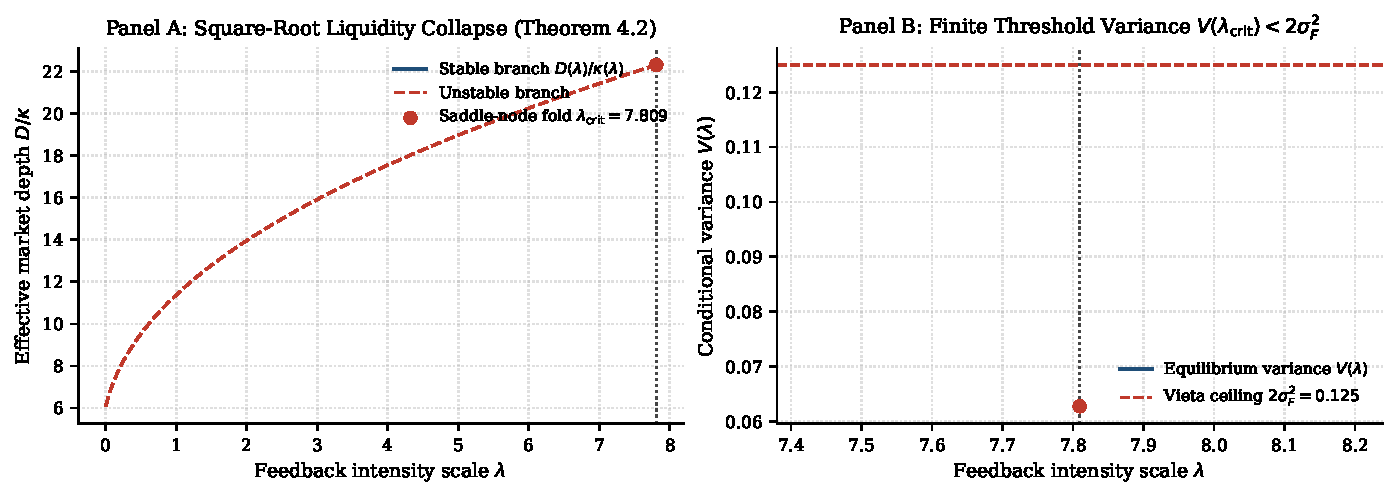
\includegraphics[width=.94\linewidth]{fig_supp_fragility_equilibrium.pdf}
\caption{Equilibrium saddle-node liquidity collapse (Panel~A) and Vieta conditional variance ceiling $V(\lambda_{\mathrm{crit}})<2\sigma_F^2$ (Panel~B) for Theorem~\ref{M-thm:fragility} ($A=0.5, \sigma_F=0.25, \sigma_\xi=0.35, \bar{a}=0.30, r=0.50, w=1.0$).}\label{fig:supp_fragility}\end{figure}

\subsection{Randomized hazard volatility interruptions and cross-venue coordination}\label{sec:jittered_auctions}
Under a deterministic halt trigger $S_t \ge \bar{s}$---and likewise under a bounded uniform trigger $\tilde{s}_{\mathrm{trig}} \sim U[\bar{s}-\delta_s, \bar{s}]$, whose conditional hazard $(\bar{s} - S_t)^{-1}$ still diverges at the upper endpoint $\bar{s}$---forward-looking dealers anticipate illiquidity lock-up as $S_t \uparrow \bar{s}$ and collapse depth prematurely \citep{subrahmanyam1994}. Mitigating pre-trigger magnet spikes favors a stress-thresholded excursion/imbalance hazard intensity $\lambda_{\mathrm{trig}}(|r_{t-1}|, \Delta_{\mathrm{imb}})\,\mathbf{1}_{\{\max(|r_{t-1}|/\sigma_0,\, \Delta_{\mathrm{imb}}/\Delta_0) \ge 1\}} > 0$ (identically zero during calm sessions) transitioning into a randomized call-auction uncrossing interval $T_{\mathrm{uncross}} = T_0 + \tilde{\epsilon}$, paired with randomized imbalance collars and cross-market LULD/futures coordination across cash equities, futures, and ETFs.

\subsection{Pre-funded countercyclical margin buffers and maker-exempt fee incidence}\label{sec:margin_scaling}
Raising margin requirements mechanically as crisis stress rises (e.g., hyperbolic stress-escalating schedules) is procyclical: margin calls during drawdowns force leveraged fire sales and accelerate liquidity spirals \citep{brunnermeier2009}. Instead, central counterparties mitigate procyclicality within EMIR RTS Art.~28 / SEC Rule~17Ad-22(e)(6) 99\% MPOR VaR constraints via a stressed-lookback floor $m_{\mathrm{floor}}^{\mathrm{stress}}$ (anchoring initial margin on a 25\%--50\% stressed historical window) plus a countercyclical anti-procyclicality (APC) buffer $b_{\mathrm{APC}}(1 - \phi(\hat\sigma_t/\sigma_{\mathrm{calm}}))$ ($\phi \in [0, 1]$ nondecreasing):
\[
  m_{\mathrm{tot}}(\hat{\sigma}_t, Q_{c,t}) = \max\bigl(m_{\mathrm{VaR},99}(\hat{\sigma}_t, Q_{c,t}),\; m_{\mathrm{floor}}^{\mathrm{stress}} + m_{\mathrm{conc}}(|Q_{c,t}|) + b_{\mathrm{APC}}\,\bigl(1 - \phi(\hat{\sigma}_t / \sigma_{\mathrm{calm}})\bigr)\bigr).
\]
While stressed-lookback $m_{\mathrm{floor}}^{\mathrm{stress}} \ge m_{\mathrm{VaR},99}$ holds, releasing $b_{\mathrm{APC}}$ offsets moderate volatility increases without procyclical margin hikes (\nolinkurl{PublicationRevision17.lean}); extreme shocks exceeding $m_{\mathrm{floor}}^{\mathrm{stress}}$ still trigger mandatory 99\% VaR escalations. Because CCP initial-margin schedules bind only on margined clearing-member positions---missing unmargined cash Securities Investment Trust Enterprises (`SITEs'), intraday-flat algorithmic desks ($Q_{c,\mathrm{EOD}}=0$), and net-omnibus customer accounts---uniform $\theta \mathbf{1}$ prudential surcharges must operate at the venue order-flow level, restricting MiFID~II RTS~8 exemptions to registered market makers and NYSE/Cboe Designated Market Makers.

\section{The supervisory decision in detail}\label{app:decisionfull}

\noindent The next results were moved from the main text (Section~\ref{M-sec:supervision}).

\begin{corollary}[Guarantee of a single halt]\label{cor:robustuniform}
In the setting of Theorem~\ref{M-n:minimax}:
\begin{enumerate}
  \item[(i)] Halting any single label $c \in \{1,\dots,K\}$ leaves worst-case post-halt budget $\max_\pi (S - u_{\pi(c)}) = S - \min_d u_d$, attained whenever $\pi(c) \in \arg\min_d u_d$ (reducing $S$ by at most $\min_d u_d$ when $u_d \ge 0$, and raising $S$ when $\min_d u_d < 0$).
  \item[(ii)] Holding dealer capacity and impact parameters $(a, \kappa)$ fixed, if $S>a$ and $a\le\bar{s}\le S$, a uniform cut to $\theta = (\bar{s} - a)/(S - a)$ achieves the ceiling $\bar{s}$ exactly in every population with budget $S$, and no policy meeting the ceiling removes less aggregate feedback than $S - \bar{s}$.
\end{enumerate}
\end{corollary}

Verified partial tags break permutation symmetry across tagged groups while preserving it within each group:

\begin{theorem}[Minimax value of partial tags]\label{n:minimaxtags}
Suppose verified tags partition the classes into groups $g = 1, \dots, G$, so the record identifies each class's group membership but cannot distinguish relabelings within any group. With the same continuous cost and convex loss in both regimes, suppose $C$ is convex and invariant to within-group permutations. Then replacing $\theta$ by the group-average policy $\bar{\theta}_g = |g|^{-1} \sum_{c \in g} \theta_c$ yields budget $a + \sum_{g=1}^G \bar{\theta}_g U_g$ ($U_g = \sum_{d \in g} u_d$) under every consistent labeling and weakly dominates $\theta$ in minimax loss. The minimax value of tags is
\[
  V_{\mathrm{tag}} = \min_{\bar{\theta}} \max_{\pi} \{\ell(S'_\pi) + C\} - \min_{(\bar{\theta}_g)_g} \max_{\pi} \{\ell(S'_\pi) + C\} \ge 0,
\]
the exact gain from tailoring policy intensities across verified groups. As in Theorem~\ref{M-n:minimax}(ii), if $C$ is strictly convex on $[0, 1]^K$, the group-uniform minimizer is unique.
\end{theorem}


This section completes Section~\ref{sec:supervision}.

\paragraph{Proof of Proposition~\ref{prop:target}.}
\begin{proof}[Proof of Proposition~\ref{prop:target}]
Part (i) follows by scaling the intensities. For (ii), expand $(1-r_c-\Delta\eta s)^{-1}$: the first three moments agree, so aggregate budgets differ by order $(\Delta\eta)^3$. Each intensity converges to $W\omega_i/(1-r_c)$, giving the stated dominant-weight gap. This exceeds the aggregate discrepancy at sufficiently small spacing. A ceiling between the two post-halt budgets reduces the action problem to testing two Gaussian mean vectors. Their common-covariance testing error is $\Phi(-\sqrt N\|h^G-h^R\|_2/(2\sigma))$; the response bound in Theorem~\ref{thm:kcohort} gives the lower bound. Part (iii) follows from continuity of $w/(1-r)$ on the declared compact parameter set and the fixed margin.
\end{proof}

\paragraph{General-$K$ scope.} The same reduction gives exponent $4K-2$ for a pair whose price responses have that moment-matching order \emph{and} whose dominant intensities have a fixed gap. Moment matching alone does not supply the gap: the symmetric odd/even binomial pair has equal maximal normalized weights. Lemma~\ref{lem:everyK} and Proposition~\ref{prop:targetK} below supply a pair with a gap for every $K$. The $K=3$ rows below are numerical examples for the Gauss and Gauss--Radau pair.

\paragraph{Explicit robustness condition.} Smooth best responses alone do not preserve separation: the constant smooth map $\Phi(M)=0$ sends both post-halt budgets to $a$. Instead assume that, over the stated action and holding horizon, $|\widetilde R_j-R_j|\le\varepsilon$ for $j\in\{G,R\}$, with $R_R<R_G$. Then
\begin{equation}\label{eq:reopt_gap}
 R_R+\varepsilon\le\bar s<R_G-\varepsilon
 \quad\Longrightarrow\quad \widetilde R_R\le\bar s<\widetilde R_G.
\end{equation}
Indeed, $\widetilde R_R\le R_R+\varepsilon$ and $\widetilde R_G\ge R_G-\varepsilon$. A nonempty robust window exists if $2\varepsilon<R_G-R_R$. This is a maintained response bound, not an equilibrium result. The same allowance must cover the alternative uniform action. At the $K=2$, $\Delta\eta=0.10$ calibration, $R_R=0.532$, $R_G=0.569909$, and $\bar s=0.55$ has margin $0.018$; an allowance $0.005$ fits within it.

\subsection{The targeted halt for every \texorpdfstring{$K$}{K}}\label{app:everyK}

Proposition~\ref{prop:target}(ii) is stated for two groups. Its argument needs two populations whose kernels agree to order $(\Delta\eta)^{2K-2}$ and whose largest groups differ at order one. This subsection supplies such a pair for every $K$.

Let $\mu$ be the uniform probability measure on $[-1,1]$, let $p_0,p_1,\ldots$ be its orthonormal polynomials, and put $\lambda_K(s)=1/\sum_{j<K}p_j(s)^2$. Call a rule \emph{admissible} if it has $K$ distinct nodes in $[-1,1]$ and integrates every polynomial of degree at most $2K-2$ exactly against $\mu$. The Gauss rule and the Gauss--Radau rule of Theorem~\ref{thm:kcohort} are admissible.

\begin{lemma}[Largest weights in the family]\label{lem:everyK}
Fix $K\ge2$.
\begin{enumerate}[label=(\roman*),itemsep=1pt]
\item An admissible rule with nodes $t_1,\ldots,t_K$ has weights $\omega_i=\lambda_K(t_i)$. In particular its weights are positive.
\item There is $c_0>0$ such that, for every $|c|\le c_0$, the zeros of $p_K-c\,p_{K-1}$ are the nodes of an admissible rule $R_c$. A point is a node of $R_c$ for at most one $c$.
\item There are $c_1\ne c_2$ in $[-c_0,c_0]$ for which $R_{c_1}$ and $R_{c_2}$ have different largest weights. Their moments of degree $2K-1$ differ.
\end{enumerate}
\end{lemma}

Parts (i) and (ii) are classical: the weights are the Christoffel numbers of $\mu$, and $p_K-c\,p_{K-1}$ is a quasi-orthogonal polynomial \citep{szego1975,gautschi2004}. We include the short proofs.

\begin{proof}
(i) Let $\ell_i$ be the Lagrange polynomials of the nodes. Each product $\ell_i\ell_j$ has degree $2K-2$, so the rule integrates it exactly: $\int\ell_i\ell_j\,d\mu=\sum_m\omega_m\ell_i(t_m)\ell_j(t_m)=\omega_i\mathbf 1\{i=j\}$. Taking $i=j$ gives $\omega_i=\int\ell_i^2d\mu>0$. So $\ell_i/\sqrt{\omega_i}$, $i=1,\ldots,K$, is an orthonormal basis of the polynomials of degree at most $K-1$, as is $p_0,\ldots,p_{K-1}$. The sum of squares of an orthonormal basis at a point does not depend on the basis, so $\sum_{j<K}p_j(s)^2=\sum_i\ell_i(s)^2/\omega_i$. At $s=t_i$ the right side is $1/\omega_i$.

(ii) The zeros of $p_K$ are real, simple and inside $(-1,1)$. Simple real zeros move continuously with the coefficients, so for $|c|\le c_0$, with $c_0$ small, $q_c=p_K-c\,p_{K-1}$ has $K$ simple zeros in $(-1,1)$. Give these nodes the interpolatory weights. Let $f$ have degree at most $2K-2$ and write $f=q_cg+\rho$ with $\deg g\le K-2$ and $\deg\rho\le K-1$. Both $p_K$ and $p_{K-1}$ are orthogonal to polynomials of degree at most $K-2$, so $\int q_cg\,d\mu=0$, and the rule integrates $\rho$ exactly and gives $q_cg$ the value zero. Hence the rule is exact for $f$. If $s$ is a zero of $q_c$ and of $q_{c'}$ with $c\ne c'$, then $p_{K-1}(s)=0$ and so $p_K(s)=0$. By the three-term recurrence a common zero of $p_K$ and $p_{K-1}$ is a zero of $p_{K-2}$, and so on down to $p_0=1$, which has none.

(iii) The reciprocal $1/\lambda_K$ is a polynomial of degree $2K-2\ge2$, so every level set of $\lambda_K$ is finite. Suppose all the rules $R_c$, $|c|\le c_0$, had the same largest weight $v$. By (i) each $R_c$ would have a node in the finite set $\{\lambda_K=v\}$, and by (ii) different values of $c$ would give different nodes. There are infinitely many $c$, so this is impossible. For the last statement, let $\nu$ be the difference of the two rules. It is supported on at most $2K$ points. If the two rules also agreed at degree $2K-1$, $\nu$ would vanish on every polynomial of degree at most $2K-1$, including the one that equals $1$ at one support point and $0$ at the others. So $\nu$ would be zero, which contradicts (ii) and the positivity of the weights.
\end{proof}

\begin{proposition}[Supervisory separation for every $K$]\label{prop:targetK}
Fix $K\ge2$ and let $R_{c_1}$ and $R_{c_2}$ be the rules of Lemma~\ref{lem:everyK}(iii), with nodes $s^j_i$, weights $\omega^j_i$ and largest weights $v_1<v_2$. Under the hypotheses of Theorem~\ref{thm:kcohort}, let economy $j\in\{1,2\}$ have $K$ groups with rates $r_c+\Delta\eta\,s^j_i$ and merged weights $W\omega^j_i$, and write $q^j_i=W\omega^j_i/(1-r_c-\Delta\eta\,s^j_i)$.
\begin{enumerate}[label=(\roman*),itemsep=1pt]
\item The response bounds of Theorem~\ref{thm:kcohort} hold for this pair: $\|h^1-h^2\|_2\le C_U(\Delta\eta)^{2K-1}$ for every horizon, and $\|h^1-h^2\|_2\ge\kappa^2W|g|(\Delta\eta)^{2K-1}$ when at least $2K+1$ taps are observed, where $g\ne0$ is the difference of the two rules at degree $2K-1$.
\item The feedback budgets satisfy $|S^1-S^2|=O((\Delta\eta)^{2K-1})$, and the largest groups satisfy $\max_iq^2_i-\max_iq^1_i=W(v_2-v_1)/(1-r_c)+O(\Delta\eta)$.
\item For sufficiently small spacing there is a nonempty interval of ceilings at which halting the largest group meets the ceiling in economy 2 and not in economy 1. For $N$ independent reset records with Gaussian noise $\sigma^2I$, a rule that makes this decision with both errors at most $1/4$ needs
\[
N\ \ge\ \bigl(2\Phi^{-1}(0.75)\,\sigma/\|h^1-h^2\|_2\bigr)^2\ \ge\ c\,\sigma^2(\Delta\eta)^{-(4K-2)} .
\]
\end{enumerate}
\end{proposition}

\begin{proof}
(i) The proof of Theorem~\ref{thm:kcohort} uses four properties of its pair: nodes in $[-1,1]$, positive weights of unit mass, equal moments up to degree $2K-2$, and a nonzero difference at degree $2K-1$. Lemma~\ref{lem:everyK} gives all four. (ii) Expanding $(1-r_c-\Delta\eta\,s)^{-1}$ in powers of $\Delta\eta$, the sum $\sum_iq^j_i$ is $W\sum_{m\ge0}(\Delta\eta)^m\mu^j_m/(1-r_c)^{m+1}$, where $\mu^j_m$ is the moment of degree $m$ of rule $j$. The moments agree for $m\le2K-2$, which gives the first statement. Each $q^j_i$ equals $W\omega^j_i/(1-r_c)+O(\Delta\eta)$, and the maximum is continuous, which gives the second. (iii) The post-halt budgets are $R^j=S^j-\kappa\max_iq^j_i$, so $R^1-R^2=\kappa W(v_2-v_1)/(1-r_c)+O(\Delta\eta)>0$ for small spacing, and any ceiling strictly between $R^2$ and $R^1$ separates the two decisions. The decision is then a test between two Gaussian mean vectors, as in the proof of Proposition~\ref{prop:target}, and (i) gives the bound.
\end{proof}

\paragraph{What is and is not shown.} The pair in Proposition~\ref{prop:targetK} is two members of the family $R_c$, not the Gauss and Gauss--Radau pair itself. For that pair Supplement Proposition~\ref{prop:maxweight} proves that the largest weights differ for every $K\ge2$, with difference $\pi/(4K^2)+O(K^{-3})$. Lemma~\ref{lem:everyK}(ii) proves admissibility only for $c$ near zero. Numerically, for $K=2,\ldots,14$ the rules $R_c$ are admissible on the whole range between the two Gauss--Radau rules, their weights equal $\lambda_K$ at the nodes to $7\times10^{-13}$, and on a grid of 41 values of $c$ the largest weight is smallest at the Gauss rule and largest at the Gauss--Radau rules (\nolinkurl{equilibrium/every_k_halt_check.py}). The counting step in part~(iii) is machine-checked (\texttt{p1\_largest\_weight\_not\_constant} in \nolinkurl{Paper1EveryKHalt.lean}), with parts (i) and (ii) and the finiteness of the level sets as hypotheses. The rest is proved on paper.


\subsection{Proof of Proposition~\ref{prop:nearcrit}}\label{app:nearcrit}

Write $D_X(z)=z-a-\kappa G_X(z)$ for economy $X$, so that $H_X=\kappa z/D_X$ and the stationary price spectrum is $f_X(\omega)=\sigma^2\kappa^2/|D_X(e^{i\omega})|^2$. Because both economies have budget $1-\epsilon$ and the same persistence, $D_A(1)=D_B(1)=\epsilon$ and $G_A(1)=G_B(1)$.

\emph{Step 1: the difference vanishes at zero frequency.} With $E=G_B-G_A$, $\Delta(z)\equiv D_B(z)-D_A(z)=-\kappa E(z)=-\kappa\,(E(z)-E(1))$, because the common budget gives $E(1)=0$; $\Delta$ does not depend on $\epsilon$. Write $E(z)=\sum_me_mz^{-m}$ with $e_m=k^B_m-k^A_m$. Then $|E(e^{i\omega})-E(1)|\le|\omega|\sum_mm|e_m|$. The rates are $r_c+\Delta\eta\,s$. Expanding $(r_c+\Delta\eta\,s)^m$ and $(1-r_c-\Delta\eta\,s)^{-1}$ in powers of $\Delta\eta$, the moments of order up to $2K-2$ of the two normalized rules cancel, so the rescaling factor satisfies $|c|\le C_0(\Delta\eta)^{2K-1}$ and $|e_m|\le2W\sum_{j\ge2K-1}\binom mj r_c^{m-j}(\Delta\eta)^j+|c|W(r_c+\Delta\eta)^m$. Summing, $\sum_mm|e_m|\le C_1(\Delta\eta)^{2K-1}$, with $C_1$ depending on $K,W,r_c$ and a bound on $\Delta\eta$. Hence $|\Delta(e^{i\omega})|\le\kappa C_1(\Delta\eta)^{2K-1}|\omega|$.

\emph{Step 2: the denominator is bounded below by $\epsilon+|\omega|$.} Let $a^*=\lim_{\epsilon\to0}a(\epsilon)$ and $D^*=D_A-\epsilon$, the denominator of economy $A$ at budget one; $D_A=D^*+\epsilon$. At budget one the closed-loop matrix $J$ of the price and the groups is entrywise nonnegative with a positive diagonal and positive first row and column (since $a^*>0$ and all weights are positive), so it is primitive. Its Perron root is $1$, it is simple, and no other eigenvalue lies on the unit circle. The zeros of $D^*$ in $|z|\ge1$ are eigenvalues of $J$, so $D^*$ has no zero on the unit circle except $z=1$, and there $D^{*\prime}(1)=1+\kappa\sum_iw_ir_i/(1-r_i)^2>0$. Hence there are $\delta,c_1,C_2,m>0$ with $|\mathrm{Im}\,D^*(e^{i\omega})|\ge c_1|\omega|$ and $\mathrm{Re}\,D^*(e^{i\omega})\ge-C_2\omega^2$ for $|\omega|\le\delta$, and $|D^*(e^{i\omega})|\ge m$ for $\delta\le|\omega|\le\pi$. For $|\omega|\le\delta$: if $\epsilon\ge2C_2\omega^2$ then $\mathrm{Re}\,D_A\ge\epsilon/2$ and $|D_A|\ge\max(\epsilon/2,c_1|\omega|)$; if $\epsilon<2C_2\omega^2$ then $|D_A|\ge c_1|\omega|$ and $\epsilon<2C_2\delta|\omega|$. In both cases $|D_A(e^{i\omega})|\ge c_2(\epsilon+|\omega|)$. For $|\omega|\ge\delta$ and $\epsilon\le m/2$, $|D_A|\ge m/2$. So $|D_A(e^{i\omega})|\ge c_3(\epsilon+|\omega|)$ on $[-\pi,\pi]$ for all $\epsilon\le\epsilon_1$. These constants can be taken uniform in $\Delta\eta\in(0,\Delta\eta_0]$. As $\Delta\eta\to0$ the kernel of $A$ converges to that of the one-group economy at rate $r_c$ in the norm $\sum_m(1+m^2)|k_m|$, so $D^*$ and its first two derivatives converge uniformly on the circle. The limit has the same properties: its closed-loop matrix is primitive with Perron root $1$, and its derivative at $1$ is at least $1$. Hence $c_1$, $C_2$, $\delta$ and $m$ can be chosen for the limit and kept, after halving $c_1$ and $m$ and doubling $C_2$, for all small $\Delta\eta$.

\emph{Step 3: the bound.} By Steps 1 and 2, $\rho(\omega)=|\Delta/D_A|\le\kappa C_1(\Delta\eta)^{2K-1}|\omega|/(c_3(\epsilon+|\omega|))\le C_3(\Delta\eta)^{2K-1}$, uniformly in $\epsilon$ and $\omega$. The ratio of spectra is $u=f_B/f_A=|D_A/D_B|^2=|1+\Delta/D_A|^{-2}$, so for $\rho\le1/8$, $|u-1|\le4\rho$. The divergence rate of stationary Gaussian processes is $D_\epsilon(B\|A)=\frac1{4\pi}\int_{-\pi}^{\pi}(u-1-\log u)\,d\omega$, and $u-1-\log u\le2(u-1)^2$ for $|u-1|\le1/2$. Hence $D_\epsilon(B\|A)\le16C_3^2(\Delta\eta)^{4K-2}$ for all $\epsilon\le\min(\epsilon_0,\epsilon_1)$ and all $\Delta\eta$ small enough that $C_3(\Delta\eta)^{2K-1}\le1/8$. For $\epsilon_1<\epsilon\le\epsilon_0$ both economies are uniformly stable, so $|D_A|$ is bounded below by a constant on the circle, while $|\Delta|=\kappa|E(e^{i\omega})|=O((\Delta\eta)^{2K-1})$; Step~3 then applies with this lower bound in place of Step~2. Steps 2 and 3 are machine-checked, with Whittle's formula, Step 1 and the local properties of $D^*$ as hypotheses (\texttt{p1\_nearcrit\_lower}, \texttt{p1\_ratio\_bound}, \texttt{p1\_nearcrit\_kl\_bound}, \nolinkurl{Paper1NearCritical.lean}). \qed

\paragraph{Numerical check.} For $K=2,3$, $\Delta\eta\in\{0.1,0.05,0.025\}$ and margins from $10^{-1}$ to $10^{-6}$, the ratio $D_\epsilon(B\|A)/(\Delta\eta)^{4K-2}$ increases to a finite limit as $\epsilon\to0$ ($0.27$ to $0.33$ for $K=2$, $0.51$ to $0.57$ for $K=3$; \nolinkurl{nearcrit_admissible.py}). At $\Delta\eta=0.1$ the rescaling factor is $1+c$ with $c=1.6\times10^{-3}$ for $K=2$ and $c=1.6\times10^{-5}$ for $K=3$. Without the rescaling the budgets differ by $4.8\times10^{-4}$ and $4.8\times10^{-6}$; the divergence rate then grows roughly like $\epsilon^{-1}$ until $\epsilon$ reaches that gap, and levels off, which is the budget difference becoming visible.


\paragraph{Finite samples.} The proposition bounds the information per observation; the same bound holds for every record length.

\begin{proposition}[Near instability, finite samples]\label{prop:nearcritn}
Under the conditions of Proposition~\ref{prop:nearcrit}, with $C_3(\Delta\eta)^{2K-1}\le1/8$, the divergence between the laws of $n$ consecutive stationary observations of the two economies is at most $16nC_3^2(\Delta\eta)^{4K-2}$, for every $n$ and uniformly in the margin $\epsilon$.
\end{proposition}

\begin{proof}
The covariance of $n$ consecutive observations is the Toeplitz matrix $T_n(f)$ of the spectral density, and $x^\top T_n(f)x=\frac1{2\pi}\int|\hat x(\omega)|^2f(\omega)\,d\omega$. Step~3 gives $|u-1|\le4\rho$ for $u=f_B/f_A$ at every frequency, so $(1-4\rho)T_n(f_A)\preceq T_n(f_B)\preceq(1+4\rho)T_n(f_A)$, and every eigenvalue $\lambda_k$ of $T_n(f_A)^{-1}T_n(f_B)$ lies within $4\rho$ of one. The divergence is $\frac12\sum_k(\lambda_k-1-\log\lambda_k)\le\frac12n\cdot2(4\rho)^2=16n\rho^2$, using $u-1-\log u\le2(u-1)^2$ for $|u-1|\le1/2$.
\end{proof}

The eigenvalue step is machine-checked (\texttt{p1\_nearcrit\_finite\_sample}, \nolinkurl{Paper1OpenResolved.lean}); the Toeplitz sandwich is on paper. Numerically, the exact divergence of $n$ consecutive stationary observations lies between $98.0\%$ and $99.8\%$ of $n$ times the per-observation rate for $K=2$, $\Delta\eta\in\{0.1,0.2\}$, $\epsilon\in\{10^{-1},10^{-2},10^{-3}\}$ and $n\in\{250,1000,4000\}$ (\nolinkurl{nearcrit_admissible.py}). In every such case all eigenvalues lie in the band of the proof, and the divergence is below the bound.

\section{Which questions prices answer cheaply}\label{app:questions}

The cost results of Section~\ref{sec:cost} concern composition. This section asks the same question of every linear question about the population, and finds a dichotomy: some questions are answered at the usual statistical rate whatever the number of groups and the spacing of their memories, some cannot be answered at all without a bound on memory, and the cost of each is the value of a problem of polynomial approximation. The results also appear in the first author's thesis (in preparation); the proofs below are complete.

\paragraph{Setting.} Write $M=\sum_iw_i\delta_{r_i}$ for the merged measure, so that $k_m=\int r^m\,dM$, and $\mathcal M(\bar r,\bar W)$ for the positive measures on $[0,\bar r]$ of total mass at most $\bar W$, with $\bar r<1$ a memory bound. A \emph{linear question} is $F_g(M)=\int g\,dM$ with $g$ continuous on $[0,\bar r]$; examples are a single tap ($g(r)=r^m$), the discounted feedback ($g(r)=(1-\beta r)^{-1}$, $\beta<1$), and the total feedback weight $\Phi=\int dM/(1-r)=\sum_m k_m$, which with $a$ and $\kappa$ fixes the feedback budget $S=a+\kappa\Phi$. The observer runs $N$ independent experiments, each returning the first $L$ kernel taps with independent $N(0,\sigma^2)$ noise. One way to obtain them is a steering probe that holds the price at a unit impulse (as in the proof of \citealp[Theorem~S6.7]{niroula2026full}), with aggregate feedback flow observed: the flow at date $t+1$ is then $k_t$. Price records are discussed at the end of the section. For accuracy $\epsilon>0$ and level $1-\alpha$, $N_{\rm cert}(\epsilon;F_g)$ is the least $N$ for which some interval built from the data has half-width at most $\epsilon$ and covers $F_g(M)$ with probability at least $1-\alpha$ for every $M\in\mathcal M(\bar r,\bar W)$.

For $g(r)=\sum_ta_tr^t$ write $\tau_g(T)=\bar W\sup_{r\le\bar r}|\sum_{t\ge T}a_tr^t|$, $A_g(T)=\sum_{t<T}a_t^2$, $T_g(\epsilon)=\min\{T\ge1:\tau_g(T)\le\epsilon/2\}$, and $E_T(g)=\min_{\deg p<T}\max_{[0,\bar r]}|g-p|$. For $c\in\mathbb R^L$ put $p_c(r)=\sum_{t<L}c_tr^t$, and for a function $h$ on $[0,\bar r]$ put $\mathcal R(h)=(\sup h)_++(-\inf h)_+$, which is at least $\|h\|_\infty$. The modulus of the question is
\[
 \omega_L(\delta)=\sup\bigl\{F_g(M_1)-F_g(M_0):\ M_0,M_1\in\mathcal M(\bar r,\bar W),\ \|k_{0:L}(M_1)-k_{0:L}(M_0)\|_2\le\delta\bigr\},
\]
the largest difference in the answer between two populations whose observed taps differ by at most $\delta$.

\begin{theorem}[The cost of a linear question]\label{thm:questions}
Let $z_\beta$ be the standard normal $\beta$-quantile and $\alpha\in(0,1/2)$.
\begin{enumerate}[label=(\roman*)]
\item \emph{Upper bound.} If $L\ge T_g(\epsilon)$, then $N_{\rm cert}(\epsilon;F_g)\le\lceil4z_{1-\alpha/2}^2\sigma^2A_g(T_g(\epsilon))\epsilon^{-2}\rceil$.
\item \emph{Truncation is necessary.} For every $T$ there are $M,M'\in\mathcal M(\bar r,\bar W)$ whose first $T$ taps coincide and with $|F_g(M)-F_g(M')|\ge2\bar WE_T(g)$; any certificate that uses only the first $T$ taps has worst-case half-width at least $\bar WE_T(g)$.
\item \emph{Long memory makes some questions impossible.} On the positive measures on $[0,1)$ of mass at most $\bar W$, with no memory bound, if $\limsup_{r\uparrow1}|g(r)|\sqrt{1-r}=\infty$, then no finite $N$ certifies $F_g$ to any finite accuracy.
\item \emph{Exact cost.} For every depth $L$ and $\delta>0$,
\[
 \omega_L(\delta)=\min_{c\in\mathbb R^L}\bigl\{\delta\|c\|_2+\bar W\,\mathcal R(g-p_c)\bigr\},
\]
and $\omega_L(0)=2\bar WE_L(g)$. If $N$ experiments certify $F_g$ to half-width $\epsilon$ at level $1-\alpha$, then $\omega_L(2z_{1-\alpha}\sigma/\sqrt N)\le2\epsilon$; conversely, if $\omega_L(2z_{1-\alpha/2}\sigma/\sqrt N)\le2\epsilon$, an affine interval $\sum_tc_t\bar k_t+b\pm\epsilon$ certifies $F_g$ with $N$ experiments. With $N_\omega(\epsilon)=\min\{N:\omega_L(2z_{1-\alpha}\sigma/\sqrt N)\le2\epsilon\}$ and $\lambda_\alpha=z_{1-\alpha/2}/z_{1-\alpha}$,
\[
 N_\omega(\epsilon)\le N_{\rm cert}(\epsilon;F_g)\le N_\omega(\epsilon/\lambda_\alpha).
\]
\end{enumerate}
\end{theorem}

\begin{proof}
(i) Let $\bar k_t$ be the average of the $N$ replicates of tap $t$, and $T=T_g(\epsilon)$. The estimator $\hat F=\sum_{t<T}a_t\bar k_t$ has mean $\sum_{t<T}a_tk_t$ and variance $\sigma^2A_g(T)/N$. Its bias is $|\sum_{t\ge T}a_tk_t|=|\int\sum_{t\ge T}a_tr^t\,dM|\le\tau_g(T)\le\epsilon/2$ for every $M$ in the class. So $\hat F\pm(\epsilon/2+z_{1-\alpha/2}\sigma\sqrt{A_g(T)/N})$ covers $F_g(M)$ with probability at least $1-\alpha$, and its half-width is at most $\epsilon$ once $z_{1-\alpha/2}\sigma\sqrt{A_g(T)/N}\le\epsilon/2$.

(ii) If $E_T(g)=0$, take $M=M'=0$. Otherwise, by duality for best uniform approximation, $E_T(g)=\max\int g\,d\nu$ over signed measures $\nu$ on $[0,\bar r]$ of total variation at most one that annihilate every polynomial of degree below $T$. Take a maximizer and write $\nu=\nu^+-\nu^-$. Orthogonality to constants gives $\nu^+([0,\bar r])=\nu^-([0,\bar r])=:c\le1/2$. The measures $M=(\bar W/c)\nu^+$ and $M'=(\bar W/c)\nu^-$ lie in the class, their first $T$ moments, which are their first $T$ taps, coincide, and $F_g(M)-F_g(M')=(\bar W/c)E_T(g)\ge2\bar WE_T(g)$. Two populations that produce identically distributed data cannot both be covered by an interval of half-width below half the difference of their answers.

(iii) Compare $M_0=0$ with $M_1=c\delta_r$ for $c=d\sigma\sqrt{(1-r^2)/N}$ and $0<d<1-2\alpha$. For $r$ near one the mass is at most $\bar W$, and the KL even using all taps is bounded by $Nc^2/[2\sigma^2(1-r^2)]=d^2/2$. Pinsker gives total variation at most $d/2$. The answers differ by $c|g(r)|$, which is unbounded along a sequence $r\uparrow1$. For separation greater than $2\epsilon$, the event that the certificate contains $F_g(M_0)$ would force total variation at least $1-2\alpha$.

(iv) \emph{Duality.} For any $c\in\mathbb R^L$ and any admissible pair, with $h=g-p_c$,
\[
 F_g(M_1)-F_g(M_0)=\int h\,dM_1-\int h\,dM_0+\langle c,k_{0:L}(M_1)-k_{0:L}(M_0)\rangle\le\bar W\mathcal R(h)+\delta\|c\|_2,
\]
because $\int h\,dM_1\le\bar W(\sup h)_+$ and $-\int h\,dM_0\le\bar W(-\inf h)_+$ for measures of mass at most $\bar W$. So $\omega_L(\delta)$ is at most the minimum. For the reverse inequality let $\mu=(M_0,M_1)$ and $\Lambda(\mu,c)=\int h\,d(M_1-M_0)+\delta\|c\|_2$. Since $\inf_c\{\delta\|c\|_2-\langle c,v\rangle\}$ is $0$ if $\|v\|_2\le\delta$ and $-\infty$ otherwise, $\omega_L(\delta)=\sup_\mu\inf_c\Lambda(\mu,c)$. The set $\mathcal M(\bar r,\bar W)^2$ is convex and weak-$*$ compact, $\Lambda$ is affine and weak-$*$ continuous in $\mu$ (as $h$ is continuous) and convex and continuous in $c$, so Sion's minimax theorem gives $\omega_L(\delta)=\inf_c\sup_\mu\Lambda(\mu,c)$. The inner supremum is $\bar W\mathcal R(g-p_c)+\delta\|c\|_2$, attained by mass $\bar W$ at a maximizer of $h$ if $\sup h>0$ and at a minimizer if $\inf h<0$. For $\delta>0$ the objective is convex, continuous and coercive in $c$, so the infimum is attained. At $\delta=0$ the same argument gives $\omega_L(0)=\inf_c\bar W\mathcal R(g-p_c)$; adding a constant to $p_c$ makes $g-p_c$ change sign, where $\mathcal R$ is the oscillation, so the infimum is $\bar W$ times the least oscillation of $g-p$ over polynomials of degree below $L$, which is $2\bar WE_L(g)$.

\emph{Lower bound.} The averages $\bar k=(\bar k_0,\ldots,\bar k_{L-1})$ are sufficient and distributed as $N(k_{0:L}(M),(\sigma^2/N)I_L)$, so the total variation distance between the data laws of two populations is $2\Phi_{\mathcal N}(\sqrt N\|\Delta k\|_2/(2\sigma))-1$, with $\Phi_{\mathcal N}$ the standard normal distribution function. For an admissible pair with $\|\Delta k\|_2<2z_{1-\alpha}\sigma/\sqrt N$ this is below $1-2\alpha$. If their answers differed by more than $2\epsilon$, an interval of half-width $\epsilon$ covering each with probability $1-\alpha$ would separate the two laws with total variation at least $1-2\alpha$, as in (iii). Hence $\omega_L(t)\le2\epsilon$ for every $t<2z_{1-\alpha}\sigma/\sqrt N$. The modulus is concave (the admissible pairs form a convex set and the constraint is a norm), finite and nondecreasing, hence continuous on $(0,\infty)$, so $\omega_L(2z_{1-\alpha}\sigma/\sqrt N)\le2\epsilon$.

\emph{Upper bound.} Put $\delta=2z_{1-\alpha/2}\sigma/\sqrt N$, let $c$ attain the minimum in the dual form and $h=g-p_c$. The interval $\sum_tc_t\bar k_t+b\pm\epsilon$ with $b=\bar W[(\sup h)_+-(-\inf h)_+]/2$ has bias at most $\bar W\mathcal R(h)/2$ for every population, by the bounds in the duality step, and normal noise with standard deviation $\sigma\|c\|_2/\sqrt N$. It covers $F_g$ with probability at least $1-\alpha$ whenever $\epsilon\ge\bar W\mathcal R(h)/2+z_{1-\alpha/2}\sigma\|c\|_2/\sqrt N=\omega_L(\delta)/2$.

\emph{Sandwich.} The left inequality restates the lower bound. Concavity and $\omega_L(0)\ge0$ give $\omega_L(\lambda t)\le\lambda\omega_L(t)$ for $\lambda\ge1$. If $\omega_L(2z_{1-\alpha}\sigma/\sqrt N)\le2\epsilon/\lambda_\alpha$, then $\omega_L(2z_{1-\alpha/2}\sigma/\sqrt N)\le2\epsilon$, and the upper bound applies.
\end{proof}

Part~(iv) has the structure of the classical theory of estimating a linear functional over a convex class \citep{donoho1994}: one modulus governs both the lower bound and an affine interval. What is specific to this market is the dual form. The cost of a question about the traders is the value of a problem of polynomial approximation of $g$ on the memory range, in which the coefficients are penalized because each multiplies a noisy tap. The number of groups and the spacing of their memories do not enter.

\begin{proposition}[Which questions are parametric]\label{prop:parametric}
Let $\omega_\infty(\delta)=\inf_L\omega_L(\delta)$. Then $\sup_{0<\delta\le1}\omega_\infty(\delta)/\delta<\infty$, so that $N_{\rm cert}(\epsilon;F_g)=O(\sigma^2\epsilon^{-2})$ with observation depth $L$ of order $\log(1/\epsilon)$, if and only if $g$ agrees on $[0,\bar r]$ with a power series $\sum_ta_tr^t$ whose coefficients are square summable. When $g$ is a power series on $[0,\bar r]$ with $\bar r>0$, this is the condition $\sum_ta_t^2<\infty$ on its Taylor coefficients.
\end{proposition}

\begin{proof}
If $a\in\ell^2$, take $c=(a_0,\ldots,a_{L-1})$. By Cauchy--Schwarz, $\mathcal R(g-p_c)\le2\sup_{r\le\bar r}|\sum_{t\ge L}a_tr^t|\le2\|a\|_2\bar r^L/\sqrt{1-\bar r^2}$, so $\omega_L(\delta)\le\delta\|a\|_2+2\bar W\|a\|_2\bar r^L/\sqrt{1-\bar r^2}$, which is at most $C\delta$ once $L\ge\log(1/\delta)/\log(1/\bar r)$; Theorem~\ref{thm:questions}(iv) then gives the parametric cost. Conversely, suppose $\omega_\infty(\delta)\le C\delta$ for $\delta\in(0,1]$. For $\delta_n=1/n$ choose $L_n$ and $c^{(n)}\in\mathbb R^{L_n}$ with $\delta_n\|c^{(n)}\|_2+\bar W\mathcal R(g-p_{c^{(n)}})\le2C\delta_n$. Then $\|c^{(n)}\|_2\le2C$ and $\|g-p_{c^{(n)}}\|_\infty\le2C\delta_n/\bar W\to0$. Padded with zeros, the $c^{(n)}$ are bounded in $\ell^2$, so a subsequence converges weakly to some $a\in\ell^2$. For each $r\in[0,\bar r]$ the sequence $(r^t)_t$ lies in $\ell^2$, so $p_{c^{(n)}}(r)=\langle c^{(n)},(r^t)\rangle\to\sum_ta_tr^t$ along the subsequence, while $p_{c^{(n)}}(r)\to g(r)$. Power series that agree on an interval are equal, which gives the last sentence.
\end{proof}

\paragraph{Where the questions of this paper sit.} A single tap and the discounted feedback have square-summable coefficients and are parametric: they cost of order $\sigma^2\epsilon^{-2}$ experiments however many groups there are and however close their memories. Square-summable power series are the restrictions of the Hardy space $H^2$ of the unit disc, whose functions grow at most like $(1-r)^{-1/2}$ as $r\uparrow1$; that is exactly the growth beyond which part~(iii) rules out certification without a memory bound. The total feedback weight $\Phi$, which fixes the feedback budget and with it stability and worst-case transient loss, has $a_t\equiv1$ and sits on the boundary: \citet{niroula2026b} show that it costs $\sigma^2\epsilon^{-2}\log(1/\epsilon)$ experiments and that the logarithm cannot be removed. Composition sits at the far end. The weight of a group is not a linear functional of $M$ at all, and by Theorem~\ref{thm:kcohort} its cost grows like $(\Delta\eta)^{-(4K-2)}$. Market-wide questions are cheap; questions about who trades are not.

\paragraph{Price records.} The first $T+1$ impulse price taps are determined by the first $T$ kernel taps, so exact-equality counterexamples transfer to that depth. With known $(a,\kappa)$ and a fixed depth the triangular inverse is smooth, giving a fixed-dimensional plug-in estimate from repeated noisy price responses. This estimate has dependent, generally non-Gaussian errors. The modulus and confidence intervals here apply to direct kernel-tap measurements. For a single passive record, least-squares autoregression on logarithmically many lags gives such growing-depth guarantees (Main Theorem~\ref{M-n:passiveupper}).

\paragraph{Machine check.} For finite populations, the weak-duality half of (iv), the affine estimate of (i), the earlier narrower algebraic impossibility comparison and the parametric direction of Proposition~\ref{prop:parametric} correspond to declarations (\texttt{p1\_question\_weak\_duality}, \texttt{p1\_question\_truncation\_error}, \texttt{p1\_long\_memory\_impossible}, \texttt{p1\_parametric\_modulus}, \nolinkurl{Paper1QuestionsCost.lean}). The lower half of (iv), part (ii) and the converse of the proposition rest on Sion's minimax theorem, duality for best uniform approximation and weak compactness in $\ell^2$, and are proved on paper. The extended confidence range in (iii) is proved on paper.

\paragraph{Numerical check.} With two groups at memories $0.5\pm\Delta\eta$, the error of the truncated estimator of the discounted feedback ($\beta=0.9$) from noisy taps does not depend on $\Delta\eta$, while the error of the weights by Prony's method grows like $(\Delta\eta)^{-3}$: fitted slopes $-0.02$ and $-3.02$ over $\Delta\eta\in\{0.2,0.1,0.05\}$, 2,000 replications each (repository script \nolinkurl{reproduce.py}).


\subsection{Elastic outside options and dynamic revelation audits}\label{sec:elastic_exit}
Theorem~\ref{M-n:minimax} establishes minimax optimality of uniform cuts when active groups remain in the venue on $[0, 1]^K$. If anonymous groups possess heterogeneous elastic outside options (exiting to offshore or dark venues whenever $\theta_c < \underline{\theta}_i$), an asymmetric schedule straddling $\underline{\theta}_i$ can achieve lower worst-case loss than a flat cut; restoring permutation-invariant optimality then requires conditioning retention schedules on observable liquidity-supply metrics. Similarly, to prevent multi-account shell splitting on the label simplex in Section~\ref{app:relabel}, linear per-dollar penalties do not suffice; the mechanism must combine strictly superadditive or per-account beneficial-owner registration fees with volume- and price-excursion-contingent audit probabilities $\pi_{\mathrm{audit}}(V_c, |\Delta p|)$ and clawbacks satisfying \citet{border1987} monotone likelihood conditions, rendering multi-entity splitting strictly suboptimal.

\subsection{Non-Gaussian identification and bispectral polyspectra}\label{sec:bispectrum}
Second-order power spectra $f(\omega) = \sigma^2 |B(e^{-i\omega})|^2$ depend only on $|B(e^{-i\omega})|$ and therefore cannot distinguish minimum-phase from non-minimum-phase transmission-zero reflections ($z_0$ versus $1/\bar{z}_0$) in the innovation representation. When innovations have non-zero third cumulant ($\E[\varepsilon_t^3] = \gamma_3 \neq 0$), the bispectrum
\[
  f_3(\omega_1, \omega_2) = \frac{\gamma_3}{(2\pi)^2} B(e^{-i\omega_1}) B(e^{-i\omega_2}) B(e^{i(\omega_1 + \omega_2)})
\]
recovers the bispectral phase $\psi(\omega_1, \omega_2) = \arg B(e^{-i\omega_1}) + \arg B(e^{-i\omega_2}) - \arg B(e^{-i(\omega_1 + \omega_2)})$ \citep{brillinger1965,hinich1982}, resolving transmission-zero reflections. However, for minimum-phase populations whose feedback memory poles $r_i \in r_c + \Delta\eta[-1, 1]$ collide while matching moments $0, \dots, 2K-2$, Taylor expansion of $f_3$ retains leading discrepancy $O((\Delta\eta)^{2K-1})$, so under non-Gaussian innovation laws satisfying sequential quadratic location-KL regularity ($\mathrm{KL}(p(\cdot - \delta)\|p) \le C_{\mathrm{loc}}\delta^2$) replacing the Gaussian KL step of Section~\ref{app:univirr} (Theorem~\ref{n:univ}), the local $(\Delta\eta)^{-(4K-2)}$ sample-complexity barrier continues to hold.

\section{Surveillance over time and against strategic traders}\label{app:dynamic}

The cost results treat the population as fixed. Real populations drift: algorithms enter, exit and are retuned, some of them in response to the supervision itself, and the groups being watched choose how to trade. This section bounds detection in any equilibrium in which surveillance without tags pushes algorithms together, and gives the rate at which the supervisor learns when one group best-responds to a fixed test. A speed limit on tracking a moving population and a floor on what probing can learn about traders who learn from prices are in the full working paper \citep{niroula2026full}.

\subsection{A surveillance and hiding game}

A group that expects to be targeted once identified may choose to trade like its neighbors. Consider two untagged groups and let one of them choose the distance $\delta\in(0,\delta_0]$ between its memory and its neighbor's, where $\delta_0$ is the distance of its preferred strategy and moving away from it costs $k(\delta_0-\delta)^2$. A supervisor with $N$ observations tests, with false-alarm probability $\alpha$, the null that the group trades like its neighbor. At leading order its detection probability depends on the data and the distance through $cN\delta^n$, with $n=4$ against the closest economy in the null (Theorem~\ref{M-n:paradox}); write it $P_{\rm d}(cN\delta^n)$, with $P_{\rm d}$ continuous and nondecreasing and $P_{\rm d}(0)\le\alpha$. Detection costs the group $L>0$. Tags, if the supervisor imposes them, make the group's weight identifiable at a cost that does not depend on $\delta$ (Theorem~\ref{thm:partial}).

\begin{proposition}[Surveillance and hiding]\label{prop:hidegame}
Let $\delta^*(N)$ minimize $k(\delta_0-\delta)^2+LP_{\rm d}(cN\delta^n)$ over $[0,\delta_0]$, with $n>0$.
\begin{enumerate}[label=(\roman*),itemsep=1pt]
\item \emph{Crowding.} If $P_{\rm d}$ is differentiable at $cN\delta_0^n$ with positive derivative, then $\delta^*(N)<\delta_0$.
\item \emph{Surveillance without tags is self-limiting.} $\limsup_{N\to\infty}P_{\rm d}(cN\delta^*(N)^n)\le\alpha+k\delta_0^2/L$. When the stakes are high, $L\gg k\delta_0^2$, the group is detected about as often as a false alarm, however much data the supervisor has.
\item \emph{Tags remove crowding.} If the detection probability does not depend on $\delta$, then $\delta^*=\delta_0$.
\item \emph{Many groups.} Let $M\ge2$ untagged groups choose memory positions $p_g$, group $g$ paying $k_g(p_g-p^\circ_g)^2+L_gP_{\rm d}(cN\delta_g^n)$, where $p^\circ_g$ is its preferred position and $\delta_g$ its distance to the nearest other group. In every Nash equilibrium (existence is not established here) in which the distance $\Delta_g$ from $p^\circ_g$ to the nearest other group's position stays bounded as $N$ grows, $\limsup_{N\to\infty}P_{\rm d}(cN\delta_g^n)\le\alpha+k_g\limsup_N\Delta_g^2/L_g$ for every group.
\end{enumerate}
\end{proposition}

\begin{proof}
(i) The derivative of the objective at $\delta_0$ is $ncLN\delta_0^{n-1}P_{\rm d}'(cN\delta_0^n)>0$, so a small move below $\delta_0$ lowers it. (ii) For any $b>0$ and $N$ large enough that $b(cN)^{-1/n}\le\delta_0$, optimality against $\delta=b(cN)^{-1/n}$ gives $LP_{\rm d}(cN\delta^{*n})\le k(\delta_0-b(cN)^{-1/n})^2+LP_{\rm d}(b^n)\le k\delta_0^2+LP_{\rm d}(b^n)$. Letting $b\to0$ and using continuity of $P_{\rm d}$ at zero gives the bound. (iii) The cost $k(\delta_0-\delta)^2$ is minimized at $\delta_0$. (iv) Holding the others' positions fixed, group $g$ can move to within $b(cN)^{-1/n}$ of its nearest neighbor, at cost at most $k_g(\Delta_g+b(cN)^{-1/n})^2$ and detection probability at most $P_{\rm d}(b^n)$, because $P_{\rm d}$ is nondecreasing. Equilibrium gives $L_gP_{\rm d}(cN\delta_g^n)\le k_g(\Delta_g+b(cN)^{-1/n})^2+L_gP_{\rm d}(b^n)$; letting $N\to\infty$ and then $b\to0$ gives the bound.
\end{proof}

The proposition gives the paper's results on cost a strategic reading. More data without tags make high-stakes algorithms trade alike, and so make composition harder to learn, while the detection probability stays near the false-alarm level. Tags undo the crowding. Two predictions follow that algorithm-level data could test: where algorithm identification is introduced, the dispersion of memory rates across algorithm classes should rise; and in untagged markets, the memories of strategies with the most to lose from targeting should converge as surveillance improves. With the Gaussian test and $n=4$, the optimal distance in the high-stakes case falls like $N^{-1/2}$ and detection stays at the $5\%$ false-alarm level up to $N=10^{14}$; when detection costs less than moving, $L(1-\alpha)<k\delta_0^2$, the group hides for moderate $N$ and stops hiding once data are plentiful (\nolinkurl{paradox/paradox_check.py}). With several groups, part (iv) bounds detection group by group in every equilibrium; whether an equilibrium exists, and what it looks like, is not studied here.

\subsection{The surveillance paradox}\label{app:paradox}

\noindent The next result was moved from the main text (Section~\ref{M-sec:supervision}). Endogenizing the supervisor's monitoring intensity sharpens this tension: because strategic crowding erodes detection power as $N$ grows, deterministic commitment collapses under high stakes and equilibrium auditing must be randomized.

\begin{proposition}[Endogenous monitoring commitment and mixed-strategy auditing]\label{prop:endogenous_supervisor}
In the Gaussian experiment of Theorem~\ref{M-n:paradox} ($J = c N \delta^n$, $n > 2$), suppose the supervisor chooses monitoring size $\alpha \in \{0\} \cup [\alpha_{\min}, \bar{\alpha}]$ ($\alpha_{\min} > 0$) at cost $C(\alpha) \ge c_{\min} > 0$ on $[\alpha_{\min}, \bar{\alpha}]$ ($C(0) = 0$) to maximize $V_{\mathrm{det}}(P_{\mathrm{d}}(\alpha, J) - \alpha) - C(\alpha)$, while the untagged group chooses $\delta \in [0, \delta_0]$ to minimize $L P_{\mathrm{d}}(\alpha, J) + k(\delta_0 - \delta)^2$.
\begin{enumerate}
  \item[(i)] \emph{High-stakes crowding and low-stakes separation.} Fix $\alpha \ge \alpha_{\min}$. Under high stakes $L(1 - \alpha) > k \delta_0^2$, the global minimizer for large $N$ obeys
  \[
    \delta_N^* = \left(\frac{4 k \delta_0}{n \beta L}\right)^{\frac{2}{n-2}} (c N)^{-\frac{1}{n-2}} (1 + o(1)), \qquad J_N^* = c N (\delta_N^*)^n \asymp N^{-\frac{2}{n-2}} \to 0,
  \]
  where $\beta = \sqrt{2}\phi(z_\alpha)$ for a one-sided test along a known normal direction, so $P_{\mathrm{d}}(\alpha, J_N^*) \to \alpha$ and distortion cost $k(\delta_0 - \delta_N^*)^2 \to k\delta_0^2$. Conversely, if $L(1 - \alpha) < k \delta_0^2$, full separation prevails ($\delta_N^* \to \delta_0$, $P_{\mathrm{d}} \to 1$). Without a known normal direction, a two-sided composite-null GLRT ($P_{\mathrm{d}}(J) - \alpha = c_2 J + O(J^2)$, $c_2 > 0$) slows crowding to $\delta_N^* \asymp N^{-1/(n-1)}$ and $J_N^* \asymp N^{-1/(n-1)}$ ($N^{-1/3}$ at $n=4$).
  \item[(ii)] \emph{Stackelberg collapse and simultaneous mixed-strategy auditing.} Under high stakes, if the supervisor commits to a pure $\alpha$ before $\delta$ is chosen, $P_{\mathrm{d}}(\alpha, J_N^*) - \alpha \to 0$ uniformly on $[\alpha_{\min}, \bar{\alpha}]$ drives committed net supervisory payoff strictly below zero for large $N$, forcing $\alpha_N^* = 0$. In a simultaneous-move game with $V_{\mathrm{det}}(1 - \alpha_{\min}) > C(\alpha_{\min})$ ($V_{\mathrm{det}} > c_{\min}$), no pure-strategy Nash equilibrium exists for large $N$; equilibrium requires randomized monitoring ($p^* > 0$) leaving traders indifferent. Verified class tags decouple $P_{\mathrm{d}}$ from $\delta$ and restore $\delta^* = \delta_0$.
\end{enumerate}
\end{proposition}

\begin{proof}[Proof of Proposition~\ref{prop:endogenous_supervisor}]
\emph{(i)} In the known-direction shift experiment, the Neyman--Pearson test rejects above $z_\alpha = \Phi^{-1}(1 - \alpha)$, giving $V_A(\delta) = k(\delta_0 - \delta)^2 + L \Phi(\sqrt{2 c N \delta^n} - z_\alpha)$. Differentiating yields
\[
  V_A'(\delta) = L \phi\bigl(\sqrt{2 c N \delta^n} - z_\alpha\bigr) \frac{n \sqrt{c N}}{\sqrt{2}} \delta^{\frac{n}{2} - 1} - 2 k (\delta_0 - \delta).
\]
For large $N$, on $J(\delta) \le z_\alpha^2/2$, $P_{\mathrm{d}}$ is convex in $\sqrt{2J}$, yielding a unique interior local minimizer with $\sqrt{2 c N (\delta_N^*)^n} \to 0$ solving $L \phi(z_\alpha) \frac{n \sqrt{c N}}{\sqrt{2}} (\delta_N^*)^{\frac{n-2}{2}} \sim 2 k \delta_0$, i.e., $\delta_N^* = [4 k \delta_0 / (n \beta L)]^{2/(n-2)} (c N)^{-1/(n-2)} (1 + o(1))$ with $V_A(\delta_N^*) \to k\delta_0^2 + L \alpha$; on $J(\delta) > z_\alpha^2/2$, $V_A \to L$ near $\delta_0$. Hence $\delta_N^*$ is the unique global minimizer if and only if $L(1 - \alpha) > k \delta_0^2$, whereas $L(1 - \alpha) < k \delta_0^2$ selects $\delta_N^* \to \delta_0$. Under a two-sided $\chi^2$ GLRT, odd first-order terms cancel so $P_{\mathrm{d}}(J) - \alpha = c_2 J + O(J^2)$ ($c_2 = 2 z_{\alpha/2}\phi(z_{\alpha/2})$), and the first-order condition $n L c_2 c N \delta^{n-1} \sim 2 k \delta_0$ gives $\delta_N^* \asymp N^{-1/(n-1)}$ and $J_N^* \asymp N^{-1/(n-1)}$. \emph{(ii)} Under Stackelberg commitment, for every $\alpha \ge \alpha_{\min}$, $V_{\mathrm{det}}(P_{\mathrm{d}}(\alpha, J_N^*) - \alpha) - C(\alpha) \le V_{\mathrm{det}} \sqrt{J_N^*/2} - c_{\min} < 0$ for large $N$, forcing $\alpha_N^* = 0$. In the simultaneous game, $(\alpha=0, \delta=\delta_0)$ invites a profitable supervisory deviation to $\alpha \in [\alpha_{\min}, \bar\alpha]$ when $V_{\mathrm{det}}(1-\alpha_{\min}) > C(\alpha_{\min})$, whereas any pure $\alpha \ge \alpha_{\min}$ induces crowding $\delta_N^*$ and negative supervisory surplus; hence no pure Nash equilibrium exists and randomized monitoring $p^* \in (0, 1)$ obtains.
\end{proof}


\paragraph{Proof of Theorem~\ref{M-n:paradox}.} (i) First, $\delta^*>0$. The test rejects with probability at most $\alpha$ under the closest economy in the null, and with the group at distance $\delta$ it rejects with a probability that exceeds this by at most the total variation between the two records, which is at most $\sqrt{J/2}$ (Pinsker). So moving from $0$ to a small $\delta$ changes the cost by at most $-2k\delta_0\delta+k\delta^2+L\sqrt{cN\delta^n/2}$, which is negative for small $\delta$ because $n>2$. Next, if $\delta^*\le\delta_0/3$ then $2\delta^*$ is feasible, and optimality against it gives $k(\delta_0-\delta^*)^2+LP_{\rm d}(J^*)\le k(\delta_0-2\delta^*)^2+LP_{\rm d}(cN(2\delta^*)^n)$. With $P_{\rm d}(J^*)\ge\alpha$ and Pinsker, $k[(\delta_0-\delta^*)^2-(\delta_0-2\delta^*)^2]\le L\sqrt{cN(2\delta^*)^n/2}$. The left side is at least $k\delta_0\delta^*$ (\nolinkurl{compare_double}); squaring and dividing by $\delta^{*2}$ gives the bound (\nolinkurl{paradox_lower}).
(ii) At $\delta=0$ the record is in the null, so the detection probability is at most $\alpha$; optimality against $\delta=0$ gives $L(P_{\rm d}(J^*)-\alpha)\le k[\delta_0^2-(\delta_0-\delta^*)^2]$, which is at most $k\delta_0^2$ and at most $2k\delta_0\delta^*$ (\nolinkurl{compare_zero}). If $J^*\ge\bar J$, the power envelope would give $L\beta\sqrt{\bar J}\le k\delta_0^2$, contrary to the stakes condition; so $J^*<\bar J$ and $L\beta\sqrt{cN\delta^{*n}}\le2k\delta_0\delta^*$. Squaring and dividing by $\delta^{*2}$ gives the bound (\nolinkurl{paradox_upper}).
(iii) By (ii), $\delta^*\le\delta_0/3$ once $N\ge4k^2\delta_0^2\,3^{n-2}/(L^2\beta^2c\delta_0^{n-2})$; then (i) applies too, so $\delta^{*\,n-2}$ lies between two constant multiples of $1/N$. Hence $J^*=cN(\delta^{*\,n-2})^{n/(n-2)}$ lies between constant multiples of $N\cdot N^{-n/(n-2)}=N^{-2/(n-2)}$. The detection probability is at most $\alpha+\sqrt{J^*/2}\to\alpha$, and $k(\delta_0-\delta^*)^2\to k\delta_0^2$ because $\delta^*\to0$.
(iv) For a tag-based inquiry with a memory-independent detection probability, $k(\delta_0-\delta)^2$ is minimized at $\delta_0$.
In a Gaussian shift experiment, suppose a known unit direction is normal to the null subspace and alternatives have positive projection $t$ along it. The test that rejects when this projection exceeds $z_\alpha=\Phi^{-1}(1-\alpha)$ has level $\alpha$ under every null economy and power $\Phi(t-z_\alpha)$, and $J=t^2/2$. As a function of $t=\sqrt{2J}$ the power is convex on $[0,z_\alpha]$, so it lies above its tangent at $0$: $P_{\rm d}(J)-\alpha\ge\phi(z_\alpha)\sqrt{2J}$ for $J\le z_\alpha^2/2$, and it is increasing beyond. $\square$

\paragraph{Checks.} \nolinkurl{PublicationRevision6.lean} checks the deterministic steps (\nolinkurl{compare_zero}, \nolinkurl{compare_double}, \nolinkurl{paradox_upper}, \nolinkurl{paradox_lower}) for every exponent $n\ge2$, with only Lean's standard axioms; Pinsker's inequality, unbiasedness and the power envelope enter as hypotheses. \nolinkurl{paradox/exponent_check.py} computes the divergence rate from the closed-form spectra ($a=0.3$, $\kappa=0.5$, the neighbor at memory $0.5$, both weights $0.05$, $\delta$ from $0.1$ to $0.00625$). The fitted slope of the log rate on $\log\delta$ is $4.1$ against the closest single-group economy, $4.3$ when a third, separated group is present, $2.1$ against the economy in which the group trades exactly like its neighbor, and $8.0$ for a cluster of three that shrinks together. \nolinkurl{paradox/paradox_check.py} solves the group's problem against the Gaussian test for $N$ from $10^2$ to $10^{14}$, with $k=\delta_0=c=1$, $L=50$ and $\alpha=0.05$. The two-sided bounds hold at every $N$; the fitted slopes of $\log J^*$ on $\log N$ are $-1.000$ for $n=4$ and $-0.327$ for $n=8$, against $-1$ and $-1/3$; and the detection probability at $N=10^{14}$ is $0.0500$ for both. With $n=2$ the optimal distance is $0$ at every $N$ from $10^2$ to $10^{12}$.

\paragraph{Scope.} The group takes the supervisor's test and record length as given, and only the group's distance is strategic: the neighbor does not respond, and the supervisor does not choose its test in response to the group. The theorem therefore describes a best response, not an equilibrium of a game between the supervisor and the groups. The best-response bounds use a stipulated record KL and a power envelope. A spectral slope alone supplies neither the finite-record power envelope nor a detector for an unknown normal direction. Part~(ii) needs a test whose power rises like the square root of the divergence near zero; a weaker test only strengthens the crowding. If several groups crowd together, $n$ is larger (numerically $8$ for a cluster of three), and the information falls more slowly, like $N^{-2/(n-2)}$.

\paragraph{Machine check.} Parts (ii)--(iv) of Proposition~\ref{prop:hidegame} are machine-checked (\texttt{p1\_hiding\_detection\_bound}, \texttt{p1\_hiding\_tag\_no\_crowding}, \nolinkurl{Paper1TrackingGame.lean}; \texttt{p1\_hiding\_nash\_bound}, \nolinkurl{Paper1NewsLawHiding.lean}). The analytic properties of the family $R_c$, the moment Lipschitz bounds and the closed-loop step are on paper.

\section{The hard pair: moment gap and largest weights}\label{app:openres}

This section gives the exact size of the moment gap behind the constants of Theorem~\ref{thm:kcohort} and compares the largest weights of the hard pair.

\subsection{The moment gap of the hard pair}

\begin{proposition}[The moment gap]\label{prop:gap}
Normalize the $K$-point Gauss and Gauss--Radau rules for the uniform probability on $[-1,1]$. Their moments agree up to order $2K-2$, and their moments of order $2K-1$ differ by exactly
\[
g_K=\frac{4^K}{K\binom{2K}{K}^2},\qquad \frac{\pi}{4^K}\Bigl(1+\frac1{4K}\Bigr)<g_K<\frac{\pi}{4^K}\Bigl(1+\frac1{2K}\Bigr).
\]
\end{proposition}

\begin{proof}
The Gauss rule integrates polynomials of degree $2K-1$ exactly, so its moment of order $2K-1$ is the true one. For the Gauss--Radau rule with a fixed endpoint and weight one on $[-1,1]$, the error for a function with continuous derivative of order $2K-1$ is $2^{2K-1}K[(K-1)!]^4f^{(2K-1)}(\xi)/[(2K-1)!]^3$ for some $\xi$ \citep[25.4.31]{abramowitz1964}. For $f(x)=x^{2K-1}$ the derivative is the constant $(2K-1)!$, so the error is exact, and halving it for the uniform probability gives $2^{2K-2}K[(K-1)!]^4/[(2K-1)!]^2=4^K/(K\binom{2K}{K}^2)$. The bounds follow from $4^K/\sqrt{\pi(K+1/2)}<\binom{2K}{K}<4^K/\sqrt{\pi(K+1/4)}$.
\end{proof}

The gaps $0.222$, $0.0533$ and $0.0131$ for $K=2,3,4$ reported with Theorem~\ref{thm:kcohort} are $g_2$, $g_3$ and $g_4$. The first tap at which the two price responses differ is $h_{2K}$, with $h^A_{2K}-h^B_{2K}=\pm\kappa^2Wg_K(\Delta\eta)^{2K-1}$. At leading order in $\Delta\eta$ the whole response difference is $g_K(\Delta\eta)^{2K-1}$ times a closed-loop response that depends on $K$ but not on $\Delta\eta$. So the divergence in the proof of Theorem~\ref{thm:kcohort} carries the factor $g_K^2$, and the data requirement the factor $g_K^{-2}\approx16^K/\pi^2$. This is one reason the constants grow so fast with $K$; the closed-loop factor adds more. The formula agrees with Gauss--Radau rules computed in 60-digit arithmetic to $3\times10^{-46}$ for $K\le30$, and the bounds hold for every $K\le2{,}000$ (repository script \nolinkurl{reproduce.py}).

\subsection{The largest weights of the hard pair}

\begin{proposition}[Largest weights]\label{prop:maxweight}
For every $K\ge2$, the largest weight of the normalized $K$-point Gauss--Radau rule exceeds the largest weight of the $K$-point Gauss rule. The difference is $\pi/(4K^2)+O(K^{-3})$.
\end{proposition}

\begin{proof}
Work with weights summing to $2$; normalization halves both. Write $\beta_m=\binom{2m}m4^{-m}$, so $P_{2m}(0)^2=\beta_m^2$ and $P_{2m+1}'(0)=(2m+1)P_{2m}(0)$.

\emph{Step 1: central binomial bounds.} Since $\beta_{m+1}/\beta_m=(2m+1)/(2m+2)$, the sequence $q_m=\beta_m^2(m+\frac14)$ increases, with $q_{m+1}/q_m-1=1/(4(m+1)^2(4m+1))$, and $r_m=\beta_m^2(m+\frac14+\frac1{32m})$ decreases, with $r_{m+1}/r_m-1=-(3m+4)/(4(m+1)^3(32m^2+8m+1))$. Both tend to $1/\pi$ by Wallis' formula, so $1/(\pi(m+\frac14+\frac1{32m}))\le\beta_m^2\le1/(\pi(m+\frac14))$ for $m\ge1$.

\emph{Step 2: two Sonin functions.} With $x=\cos\theta$, $u(\theta)=\sqrt{\sin\theta}\,P_K(\cos\theta)$ solves $u''+Q u=0$ with $Q(\theta)=(K+\frac12)^2+1/(4\sin^2\theta)$ \citep{szego1975}, which follows from Legendre's equation. $Q$ is symmetric about $\pi/2$ and nonincreasing on $(0,\pi/2]$. Then $S_1=u^2+u'^2/Q$ has $S_1'=-Q'u'^2/Q^2\ge0$ there, and $S_2=Qu^2+u'^2$ has $S_2'=Q'u^2\le0$. Hence on $(0,\pi)$, $S_1\le S_1(\pi/2)=P_K(0)^2+P_K'(0)^2/Q_0$ and $S_2\ge S_2(\pi/2)=Q_0P_K(0)^2+P_K'(0)^2$, with $Q_0=K^2+K+\frac12$.

\emph{Step 3: the Gauss weights from above.} At a Gauss node $u=0$ and $u'^2=\sin^3\theta\,P_K'(x)^2$, so the weight $2/((1-x^2)P_K'(x)^2)=2\sin\theta/S_2(\theta)\le2/S_2(\pi/2)$. By Step 1, the largest Gauss weight is at most $\pi G_K$, with $G_K=(K+\frac12+\frac1{8K})/Q_0$ for even $K$ and $G_K=(K-\frac12+\frac1{8(K-1)})/K^2$ for odd $K$.

\emph{Step 4: a Radau weight from below.} The interior Radau nodes are the zeros of $P_{K-1}+P_K$, with weights $(1-x)/(K^2P_{K-1}(x)^2)$ \citep[25.4.31]{abramowitz1964}. The zeros $\theta_\nu$ of $P_K$ satisfy $(\nu-\frac12)\pi/(K+\frac12)<\theta_\nu<\nu\pi/(K+\frac12)$ \citep[Theorem~6.21.2]{szego1975}, and $P_{K-1}$ changes sign between consecutive zeros of $P_K$, so some Radau node has $|x|\le\sin(5\pi/(4K+2))<d:=5/(K-\frac12)$. At that node $P_{K-1}=-P_K$, and $(1-x^2)P_K'=K(P_{K-1}-xP_K)$ gives $P_K'(x)=-KP_K(x)/(1-x)$. Substituting into $S_1$,
\[
\frac{1-x}{K^2P_{K-1}(x)^2}=\frac{\sin\theta}{K^2S_1(\theta)}\Bigl[(1-x)+\frac{K^2(1+x)+Kx+x^2/(4(1+x))}{Q(\theta)}\Bigr].
\]
With $\sin\theta\ge1-d^2$, $Q_0\le Q\le\Phi:=(K+\frac12)^2+1/(4(1-d^2))$ and $a=K^2/\Phi$, the bracket times $\sin\theta$ is at least $T_K=(1-d^2)+a(1-d^2-d^3)-d\,|1-d^2-a|-dK/Q_0$. By Step 1, $S_1(\pi/2)\le F_K/\pi$, with $F_K=2/(K+\frac12)$ for even $K$ and $F_K=2K^2/((K-\frac12)Q_0)$ for odd $K$. So the largest Radau weight is at least $\pi T_K/(K^2F_K)$.

\emph{Step 5: comparison.} For each parity, $T_K/(K^2F_K)-G_K$ is a rational function of $K$; the sign of $1-d^2-a$ is constant for $K\ge62$. Exact computation shows that its numerator and denominator have no real zero above $61.1$ and that it is positive at $K=62$. So the largest Radau weight exceeds the largest Gauss weight for every $K\ge62$. For $2\le K\le61$ the difference of the largest weights, computed in 30-digit arithmetic, is positive, the smallest being $4.2\times10^{-4}$ before normalization; a 60-digit computation confirms it up to $K=200$.

\emph{The asymptotic difference.} The interior Gauss--Radau nodes and weights are those of the $(K-1)$-point Gauss--Jacobi rule for the weight $1+x$, divided by $1+x$. Uniformly over nodes in any compact subinterval of $(-1,1)$, Gauss--Jacobi weights for the weight $(1-x)^\alpha(1+x)^\beta$ satisfy $w=\frac{\pi}{n+(\alpha+\beta+1)/2}(1-x)^{\alpha+1/2}(1+x)^{\beta+1/2}(1+O(n^{-2}))$ \citep{hale2013}. So the interior Radau weights are $\frac\pi K\sqrt{1-x^2}(1+O(K^{-2}))$, and the Gauss weights are $\frac\pi{K+1/2}\sqrt{1-x^2}(1+O(K^{-2}))$. The largest weights sit at the nodes nearest zero, where $\sqrt{1-x^2}=1-O(K^{-2})$, and the endpoint weight $2/K^2$ is smaller. Halving, the difference is $\frac\pi2(\frac1K-\frac1{K+1/2})+O(K^{-3})=\frac\pi{4K^2}+O(K^{-3})$.
\end{proof}

This explains the constant $0.79\approx\pi/4$ reported with Theorem~\ref{thm:kcohort}. The scaled gap $K^2\times$(difference) is $0.903$, $0.851$, $0.831$, $0.820$, $0.813$ and $0.809$ at $K=10,20,\ldots,60$, approaching $\pi/4=0.785$ (\nolinkurl{open_checks2.py}). The explicit bounds of Steps 3 and 4 also hold against the exact weights for every $K$ from 8 to 60, and the Radau node nearest zero is within $0.79/(K-\frac12)$ of it for $K\le300$, well inside $d$ (\nolinkurl{open_checks3.py}). The two polynomial inequalities behind Step 1 are machine-checked (\texttt{p1\_centralbinom\_q\_step}, \texttt{p1\_centralbinom\_r\_step}, \nolinkurl{Paper1OpenResolved2.lean}); the rest is on paper and in the exact computation. Proposition~\ref{prop:targetK} does not need the comparison: it covers every $K$ through the family $R_c$.

\section{Do the rates survive real market noise?}\label{sec:injection}

Theorems~\ref{thm:kcohort} and~\ref{prop:esprit} are proved for observation errors that are independent and Gaussian, and \citet{niroula2026a} checks them with Gaussian noise. Real price changes are different: one-minute returns have heavy tails, although they are almost uncorrelated from one minute to the next. To see whether the rates depend on the Gaussian assumption, we ran a pre-specified test (opened once) in which the trader groups are synthetic, with known memory spacing, and only the noise is real. Each reset experiment returns the price response to a unit impulse plus a window of consecutive one-minute log-price changes of Binance BTCUSDT, demeaned and scaled to unit variance. The changes come from 21 days, the 6th of each month from January 2025 to September 2026, that are used nowhere else in this project; their kurtosis is 19.4, against 3 for Gaussian noise. With class tagging, the experiment also returns each group's flow response, observed through independent windows of the same noise. A control arm uses i.i.d.\ Gaussian noise of the same variance. For each spacing, $N^*$ is the smallest number of experiments at which every recovered weight lies within 25\% of the smallest true weight in at least 75\% of 200 replications, using Prony's method on prices alone or the per-group regression of Proposition~\ref{prop:tagged} with tagging. The noise level and the spacing grids were fixed on Gaussian noise alone, before any real noise was downloaded.

\begin{table}[t]\centering\small
\begin{threeparttable}
\caption{Sample requirement with real Bitcoin price noise: fitted slope of $\log N^*$ in $\log\Delta\eta$}\label{tab:injection}
\begin{tabular}{lccccl}
\toprule
 & Theory & Real noise & Gaussian control & Pre-specified criterion & Result\\
\midrule
Price only, $K=2$ (H1) & $-6$ & $-6.01$ & $-6.22$ & slope in $[-7.5,-4.5]$ & pass\\
Tagged, $K=2$ (H2) & bounded & 256--724 & 256--1{,}024 & max/min $\le8$ & pass (2.8)\\
Price only, $K=3$ (H3)$^\dagger$ & $-10$ & $-9.81^\dagger$ & $-9.96$ & slope in $[-12.5,-7.5]$ & holds\\
\bottomrule
\end{tabular}
\begin{tablenotes}\footnotesize\item Synthetic groups at rates $r_c+\Delta\eta\,s$ ($s$ the $K$-point Gauss nodes; $r_c=0.6$ and $\Delta\eta$ from 0.5 to 0.125 for $K=2$, $r_c=0.5$ and $\Delta\eta$ from 0.6 to 0.25 for $K=3$), $a=0.5$, $\kappa=0.8$, total weight 0.08, $\sigma=10^{-3}$, $\sigma_f=0.02$. The test passes if H1 and H2 hold; H3 is reported either way. The tagged row gives the range of $N^*$ over the spacing grid. $^\dagger$All $K=3$ points ($>4{,}096$) and $K=2$ spacings below $0.25$ use the pre-specified covariance-matched Gaussian CLT draw (not heavy tails) because the 21-day archive contains $30{,}240$ one-minute bars; finite fourth moments ($\kappa_4 = 19.4$) inflate variance constants without altering the $(\Delta\eta)^{-(4K-2)}$ slope, whereas infinite-fourth-moment tails ($\alpha \in (2,4)$) slow passive covariance rates to $O_P(n^{-(1-2/\alpha)})$. Requirements at each spacing are in \citet{niroula2026a}. Test opened once.\end{tablenotes}
\end{threeparttable}
\end{table}

Both pre-specified hypotheses hold, so the test passes (Table~\ref{tab:injection}). With real noise, the price-only requirement for two groups rises from 64 experiments at $\Delta\eta=0.5$ to $370{,}728$ at $\Delta\eta=0.125$, a factor of about 5{,}800, and the fitted slope is $-6.01$; for three groups it is $-9.81$. Over the same grid the tagged requirement stays between 256 and 724 experiments, and it falls slightly rather than rises as the spacing shrinks. At every spacing the real-noise requirement is within one step of the grid (a factor $\sqrt2$) of the Gaussian control. The slopes are least-squares fits of $\log N^*$ on $\log\Delta\eta$ over the stated grids (seven spacings from $0.5$ to $0.125$ for two groups, five from $0.6$ to $0.25$ for three). No uncertainty interval was pre-specified; as a post hoc description, the ordinary least-squares standard errors are $0.17$ and $0.47$ with real noise ($0.12$ and $0.31$ for the Gaussian control, slopes $-6.22$ and $-9.96$), and each $N^*$ is itself read off a grid with steps of $\sqrt2$. For two groups, the last four price-only points lie above $4{,}096$ and use the normal draw, so the heavy tails enter the fit only through the first three.

The test has a limit, stated in its specification. Averages of $N$ real windows are resampled exactly up to $N=4{,}096$; beyond that they are drawn as Gaussian vectors with the real windows' covariance, as the central limit theorem suggests. Real one-minute changes are almost uncorrelated (lag-one autocorrelation between $-0.007$ and $0.009$ within the windows), so beyond $4{,}096$ the real and Gaussian arms differ little by construction. The direct evidence about heavy tails therefore comes from the points in the exact range: every tagged requirement, and the price-only requirements for two groups at the three widest spacings (64, 362 and 1{,}448 experiments, against 64, 362 and 1{,}024 with Gaussian noise). The other four price-only points for two groups, and all points for three groups, check the rate with the real noise's variance and covariance but not its tails. Averaging should make heavy tails matter less as $N$ grows, but the test does not show this.

\section{Pricing, evasion and the choice of an audit trail}\label{app:restored_policy}

\begin{proposition}[Conditional endogenous-pricing invariance]\label{prop:endogenous_kappa}
Let $\kappa=\mathcal K(\Gamma_M(\kappa))$ on a common admissible interval, with identical innovation laws, initial-state conventions and other primitives across economies. Here $\Gamma_M(\kappa)$ is the specified covariance record at a fixed impact and $\mathcal K$ is a maintained dealer rule, not a derived general equilibrium.
\begin{enumerate}[label=(\roman*)]
\item If equal merged measures imply the same map $\Gamma_M$ and the fixed point is unique (or a common selection rule depends only on that map), equal merged measures give equal selected impacts.
\item Suppose $\mathcal K$ is $L_K$-Lipschitz, each covariance map is $L_\Gamma$-Lipschitz in impact, $L_KL_\Gamma<1$, and $\sup_\kappa\|\Gamma_A(\kappa)-\Gamma_B(\kappa)\|\le\epsilon$. For existing fixed points,
\begin{equation}\label{eq:kappa_closeness}
 |\kappa_A-\kappa_B|\le\frac{L_K\epsilon}{1-L_KL_\Gamma}.
\end{equation}
Thus a covariance discrepancy of order $(\Delta\eta)^{2K-1}$ preserves that order only under these uniform conditions.
\end{enumerate}
\end{proposition}

\paragraph{Limits of the pricing extension.} Anonymous flow alone implies neither a covariance-only dealer objective nor uniqueness or continuity of its equilibrium. Multiple equilibria, threshold quote changes, private information and inventory-dependent rules are outside this proposition; for the question of invariance, Theorem~\ref{thm:eqinv} below covers them. Preserving a price-record testing bound additionally requires a uniformly Lipschitz observation law with the same nondegenerate noise; adding anonymous flow is a different statistical experiment and requires its own divergence bound. We therefore make no unconditional claim that endogenous pricing or additional aggregate-flow observations preserve the price-only lower bound.
\paragraph{Proof of Proposition~\ref{prop:endogenous_kappa}.}
 Equal maps have the same fixed-point set; uniqueness or the declared common selection yields (i). For (ii), put $d=|\kappa_A-\kappa_B|$. The fixed-point equations and the two Lipschitz bounds give $d\le L_K(L_\Gamma d+\epsilon)$. Since $1-L_KL_\Gamma>0$, rearrangement proves the displayed bound. The scalar inequality is machine checked in \nolinkurl{p1_endogenous_contraction_sensitivity}; the economic derivation and uniformity of the covariance map are assumptions, not consequences of that algebra. A discontinuous threshold pricing rule need not preserve a small discrepancy. $\square$


\begin{proposition}[Conditional limits of three evasion arguments]\label{prop:strategic}
Maintain the exogenous reporting-noise and valid-instrument assumptions of Proposition~\ref{prop:tagged}; fix the finite number of linked class labels and a uniformly stable model family.
\begin{enumerate}[label=(\roman*)]
\item For a fixed split $u_{i,m}=\alpha_{i,m}u_i$ with known common ownership, independent mean-zero reporting errors and $\alpha_{i,m}\ge\underline\alpha>0$, only the lagged-flow column of the population IV matrix scales. Thus $\Sigma_{i,m}=\Sigma_i\operatorname{diag}(\alpha_{i,m},1)$ and $\det\Sigma_{i,m}=\alpha_{i,m}\det\Sigma_i$. Subject to the remaining uniform moment and excitation conditions, fixed finitely many consistent sub-account estimates can be summed: the true identity is $w_i=\sum_m w_{i,m}$, and the estimated sum has sampling error. The share restriction implies $M_i\underline\alpha\le1$. This is not robustness to arbitrarily many vanishing accounts; a common estimated rate does not identify ownership.
\item Assume separately an execution cost lower bound $\mathbb E C_\zeta\ge c_\zeta\sigma_\zeta^2$ with $c_\zeta>0$ and a gross profit upper bound $\mathbb E\Pi\le\overline\Pi$ uniform in the spacing. Camouflage is unprofitable when $c_\zeta\sigma_\zeta^2>\overline\Pi$. A variance requirement of order $(\Delta\eta)^{-(4K-2)}$ requires an additional additive exogenous-noise estimation model with uniformly controlled instruments. Neither this variance requirement nor the execution bound is established for arbitrary strategic orders.
\item If intensity is scaled to $\gamma_iw_i$ while $1-r_i\ge\eta_{\min}>0$, then $q_i\le\gamma_iw_i/\eta_{\min}\to0$ as $\gamma_i\to0$. The other groups remain in the aggregate budget; reducing one contribution does not itself establish that the ceiling is met.
\end{enumerate}
\end{proposition}

\paragraph{Economic scope.} These are conditional calculations about fixed linked accounts, bounded execution costs and a persistence class. They do not solve a general equilibrium game of evasion; Proposition~\ref{M-n:relabel} solves a stylized one. In particular, endogenous orders can affect prices and invalidate the reporting-error instrument, and a persistence change can offset a reduction in weight. Adversarial account creation and response adaptation require further modeling.

\paragraph{Proof of Proposition~\ref{prop:strategic}.}
 (i) The current-price regressor column is unchanged, whereas the lagged true flow column scales by $\alpha_{i,m}$; valid independent reporting noise has zero population covariance with the instruments. Multiplicativity of determinants gives the stated factor. Summing shares at least $\underline\alpha$ gives $M_i\underline\alpha\le1$, checked in \nolinkurl{p1_sybil_share_count_bound}. For a fixed finite collection the summed estimation errors remain of order $T^{-1/2}$ under the maintained joint central limit assumptions; this asymptotic step is not newly formalized here. (ii) Subtract the cost lower bound from the uniform gross-profit upper bound. Once the former exceeds the latter, expected net profit is negative, as checked in \nolinkurl{p1_camouflage_unprofitable}. The cost coercivity and variance-to-difficulty link are explicit hypotheses, not consequences of fairness alone. (iii) Divide the scaled weight by $1-r_i\ge\eta_{\min}$; without that bound, taking $1-r_i=\gamma_i$ can keep $q_i=w_i$ constant. $\square$

\section{The disclosure game with relabeling}\label{app:relabel}

\paragraph{Proof of Proposition~\ref{M-n:relabel}.} (i) An $H$ trader's payoff is $b_H\{(1-z)y+zx\}-\gamma z^2/2=b_Hy+b_H(x-y)z-\gamma z^2/2$, strictly concave in $z$, so its maximizer on $[0,1]$ is the projection of $b_H(x-y)/\gamma$ (\nolinkurl{hide_best_response}).

(ii) Without disclosure, welfare is $mx$, maximized at $x=1$ if $m\ge0$ and $x=0$ otherwise. With an audit trail, $z=0$ and welfare $\chi yn_H+sx$ is maximized at $y=0$, $x=1$. Under class tags write $d=x-y\in[0,x]$ for the label gap. A policy with $b_Hd\ge\gamma$ makes $z^*=1$ and yields $mx-\chi\gamma/2$, less than the gap-free policy $y=x$; such policies are never optimal. For $b_Hd<\gamma$, substituting $z^*=b_Hd/\gamma$ gives
\[
W=mx+\chi\Big(ad-\frac{d^2}{2g}\Big)
\]
(\nolinkurl{tag_welfare_identity}). For fixed $x$ the bracket is concave in $d$, with maximum $a^2g/2$ at $\hat d=ag$ (\nolinkurl{label_gap_value}, \nolinkurl{label_gap_attained}). Since $\hat d=a\gamma/\{b_H(2a+b_H)\}<\gamma/b_H$, the restriction $b_Hd<\gamma$ never binds at the optimum, and the best gap is $\min\{x,\hat d\}$. The value of retention $x$ is therefore $\varphi(x)=sx-\chi x^2/(2g)$ for $x\le\hat d$ (using $m+\chi a=s$) and $\varphi(x)=mx+\chi a^2g/2$ for $x\ge\hat d$. The function $\varphi$ is concave and continuously differentiable, with $\varphi'(x)=s-\chi x/g$ below $\hat d$ and $\varphi'=m$ above it; the two derivatives agree at $\hat d$ because $s-\chi a=m$. If $m\ge0$, $\varphi$ is nondecreasing, so $x=1$ and the gap is $\min\{1,\hat d\}$, which gives the two values stated. If $m<0$, $\varphi'$ vanishes at $\hat x=sg/\chi$, and $\hat x<\hat d$ because $s<\chi a$; so $x=\min\{1,\hat x\}$, the gap is $x$, $y=0$, and the values follow. The equilibrium hiding share is $b_Hd/\gamma$ with $0<d\le\hat d$, so it is positive and at most $a/(2a+b_H)<1$ (\nolinkurl{hiding_share_lt_one}).

(iii) Each branch of $V_C$ is strictly increasing in $g$, which is proportional to $\gamma$: the interior branches are linear in $g$ with positive slope (\nolinkurl{tag_value_mono}) and the outer branches equal a constant minus $\chi/(2g)$ (\nolinkurl{outer_branch_mono}). Substitution shows that the branches agree where they meet ($ag=1$, respectively $sg=\chi$). As $g\to0$ the interior branches vanish; as $g\to\infty$ the outer branches tend to $\chi a=s-m$ (when $m\ge0$) and to $s$ (when $m<0$), which is $V_A$ in both cases. Each branch lies strictly below its limit (\nolinkurl{tags_below_audit_mnonneg}, \nolinkurl{tags_below_audit_mneg}, and directly for the outer branches). The regime comparison subtracts the fixed costs from these gains. Because $V_A-V_C(\gamma)$ falls continuously and strictly from $V_A$ to $0$, the trail strictly dominates for all finite $\gamma>0$ if the cost gap is zero, for no $\gamma>0$ if the gap is at least $V_A$, and below a unique positive finite cutoff otherwise. $\square$

\paragraph{Checks.} The Lean~4 file \nolinkurl{PublicationRevision3.lean} checks the steps named above with only Lean's three standard axioms. \nolinkurl{PublicationRevision4.lean} checks the case analysis: the bound in each of the four cases (\nolinkurl{case_mnonneg_inner}, \nolinkurl{case_mnonneg_outer}, \nolinkurl{case_mneg_inner}, \nolinkurl{case_mneg_outer}) and the dominance of complete pooling (\nolinkurl{pooling_dominated}). The closed forms are also checked by \nolinkurl{t6/t6_check.py}: on 400 random economies, maximizing welfare over a grid of $(x,y)$ never exceeds the closed form, the closed-form policy attains it, and on three economies $V_C$ rises strictly over $\gamma\in[10^{-4},10^4]$ from near zero to within $0.1\%$ of $V_A$.

\paragraph{Scope.} The proposition takes the classes' net values as given and lets only the restricted class relabel; we restrict attention to policies with $y\le x$, under which benign traders have no reason to adopt the harmful label. A uniform cut is implementable from prices (Proposition~\ref{M-n:target}); we take it to be the only restriction available without class identity. Relabeling here is account routing, as in Proposition~\ref{prop:strategic}(i); an audit trail that links sub-accounts to owners removes it. If classes are defined by measured behavior and disguise also changes harm, the model needs a joint cost of disguise and harm; Corollary~\ref{cor:relabelspacing} treats the case in which the measured statistic can be shifted without changing harm. Repeated cycles, learning about $\chi$ and enforcement costs are outside the model. (In institutional US equity trails, offshore total-return swaps $\gamma_{\mathrm{TRS}}$ and net-zero multi-desk pods inside one LEI create synthetic routing channels analogous to cheap labels in Proposition~\ref{prop:relabelK}; SEC CAT funding also remains subject to the Eleventh Circuit's July~2025 vacatur in \emph{ASA v.\ SEC}.)

\begin{corollary}[Comparative statics]\label{cor:relabelstatics}
At the interior optima of Proposition~\ref{M-n:relabel}:
\begin{enumerate}[label=(\roman*),itemsep=1pt]
\item when $m\ge0$, the optimal label gap $a\gamma/\{b_H(2a+b_H)\}$ rises with the relabeling cost and falls with the restricted traders' private gain $b_H$;
\item the equilibrium hiding share does not depend on $\gamma$: it is $a/(2a+b_H)$ when $m\ge0$ and $s/\{\chi(2a+b_H)\}$ when $m<0$, and it falls with $b_H$; when $m\ge0$ it rises with the harm $a$;
\item the gain from class tags, $\chi a^2\gamma/\{2b_H(2a+b_H)\}$ when $m\ge0$ and $s^2\gamma/\{2\chi b_H(2a+b_H)\}$ when $m<0$, rises with $\gamma$ and falls with $b_H$; when $m\ge0$ it rises with the harm $a$.
\end{enumerate}
\end{corollary}

\paragraph{Proof of Corollary~\ref{cor:relabelstatics}.} Substitute $g=\gamma/\{b_H(2a+b_H)\}$ in the closed forms of Proposition~\ref{M-n:relabel}(ii) and in the hiding share $b_Hd/\gamma$ at the optimal gap ($d=ag$ when $m\ge0$, $d=sg/\chi$ when $m<0$); the factor $\gamma$ cancels from the share. The monotonicity statements compare ratios of positive quantities (\nolinkurl{gap_antitone_gain}, \nolinkurl{hiding_share_antitone_gain}, \nolinkurl{hiding_share_monotone_harm}, \nolinkurl{tag_value_antitone_gain}, \nolinkurl{tag_value_monotone_harm}, \nolinkurl{tag_value_mono}). $\square$

The share of the restricted activity that hides is therefore set by the harm and the private gain, not by the cost of hiding: a cheaper channel leads the supervisor to narrow the gap until the same share hides. The more profitable the restricted activity, the milder the optimal restriction and the less class tags are worth.

\paragraph{Many classes.} Let classes $j=1,\ldots,K$ have shares $\chi_j$, net values $n_j$ and private gains $b_j>0$, and let the supervisor set label retentions $x\in[0,1]^K$. Class $j$ may route a share $z\in[0,1]$ of its activity through one label $k$ in a channel set $E_j$, at resource cost $c_{jk}z^2/2$ per unit of its activity. Assume each channel set is nonempty and each routing cost is positive. For a fixed selection among private best responses, write $W_C(c)$ for the supremum of welfare under class tags, $W_N=\max\{0,\sum_j\chi_jn_j\}$ for the uniform cut and $W_A=\sum_j\chi_j\max\{n_j,0\}$ for an audit trail before its cost.

\begin{proposition}[Disclosure with many classes]\label{prop:relabelK}
\begin{enumerate}[label=(\roman*),itemsep=1pt]
\item Class $j$ routes through a label $k\in E_j$ that maximizes $\psi_j(x_k-x_j,c_{jk})$, where $\psi_j(d,c)=\max_{0\le z\le1}(b_jdz-cz^2/2)$, with share $\min\{1,b_j(x_k-x_j)^+/c_{jk}\}$.
\item $W_N\le W_C(c)\le W_A$ for every cost profile.
\item \emph{Cheap channels.} If $c_{jk}=\epsilon\bar c_{jk}$ for $k\in E_j$, then
\[
\Big|W_C(c)-\max_{x\in[0,1]^K}\sum_j\chi_jn_j\max_{k\in E_j\cup\{j\}}x_k\Big|\ \le\ \epsilon\sum_j\chi_j\Big(\frac{|n_j|}{2b_j}+\frac12\Big)\max_{k\in E_j}\bar c_{jk}.
\]
As $\epsilon\to0$, class tags are worth only the value of the coarser problem in which each class receives the best retention among the labels it can reach.
\item \emph{Expensive channels.} With the same scaling, $|W_C(c)-W_A|\le\epsilon^{-1}\sum_j\chi_j(|n_j|b_j+b_j^2)/\min_{k\in E_j}\bar c_{jk}$, so $W_C(c)\to W_A$ as $\epsilon\to\infty$.
\end{enumerate}
\end{proposition}

\begin{corollary}[Behavior-based labels and memory spacing]\label{cor:relabelspacing}
Suppose labels are assigned from measured memory rates, class $j$ has rate $r_c+\Delta\eta\,s_j$, and shifting the measured rate of a unit of activity into a neighboring class's band costs $c_0(\Delta\eta)^2(s_k-s_j)^2$ without changing its economic effect. Then Proposition~\ref{prop:relabelK}(iii) applies with $\epsilon=(\Delta\eta)^2$ and $E_j$ the neighboring classes: the value of behavior-based class tags is within $O((\Delta\eta)^2)$ of the coarse value. With two classes the coarse value is the uniform cut's, so behavior-based tags lose their value as the memories approach each other, the same limit in which Theorem~\ref{M-n:cost} makes composition costly to learn from prices. Owner-linked audit trails are unaffected.
\end{corollary}

\paragraph{Proof of Proposition~\ref{prop:relabelK} and Corollary~\ref{cor:relabelspacing}.} (i) For a given channel the payoff $b_jdz-cz^2/2$ is strictly concave in $z$; its maximizer on $[0,1]$ is $\min\{1,b_jd^+/c\}$, and the class picks the channel with the largest maximum. (ii) The uniform policy $x_j\equiv x$ gives no class a reason to route and attains $x\sum_j\chi_jn_j$, so $W_C\ge W_N$. For any policy, welfare is $\sum_j\chi_j(n_je_j-\text{cost}_j)$ with effective retention $e_j\in[0,1]$ and nonnegative cost, so it is at most $W_A$. (iii) Fix $x$ and a class $j$, let $D=\max_{k\in E_j}(x_k-x_j)^+$, attained at $k^*$, and write $c^*=c_{jk^*}$. The chosen channel, with gap $d\le D$ and share $z$, pays at least what routing everything through $k^*$ would: $b_jdz-c_{jk}z^2/2\ge b_jD-c^*/2$. Since $dz\le D$, this gives $D-c^*/(2b_j)\le dz\le D$ and $c_{jk}z^2/2\le c^*/2$ (\nolinkurl{routing_near_best}). The effective retention $x_j+dz$ is therefore within $c^*/(2b_j)$ of $x_j+D=\max_{k\in E_j\cup\{j\}}x_k$ and the cost is at most $c^*/2$, so welfare at $x$ is within the stated bound of the coarse objective at $x$, uniformly in $x$; the suprema are within the same bound. (iv) The chosen share is at most $b_j/c_{jk}$, so the effective retention is within $b_j/c_{jk}$ of $x_j$; the cost is at most the gross gain $b_jdz\le b_j^2/c_{jk}$ (\nolinkurl{routing_expensive}). Welfare at $x$ is therefore within the stated bound of $\sum_j\chi_jn_jx_j$, whose maximum is $W_A$. For the corollary, substitute $c_{jk}=c_0(\Delta\eta)^2(s_k-s_j)^2$ into (iii); with two classes routing both ways the coarse objective is $(\chi_1n_1+\chi_2n_2)\max\{x_1,x_2\}$, whose maximum is $W_N$. $\square$

\paragraph{Checks.} \nolinkurl{t6/t6_check.py} also verifies (iii) and (iv) on random three-class economies with nearest-neighbor channels: over a grid of policies, the best welfare stays within the stated bounds of the coarse and audit values.

\paragraph{General primitives.} The limits in Proposition~\ref{prop:relabelK} do not need linear values or quadratic costs. Let class $j$ have share $\chi_j$ and an increasing private payoff $\pi_j$ of its effective retention with slopes in $[\beta_j,B_j]$, $0<\beta_j\le B_j$; let routing a share $z$ through label $k\in E_j$ cost $c_{jk}C(z)$ per unit, with $C$ continuous, $C(0)=0$, $C$ strictly increasing and $C(z)\ge\kappa_Cz^2$ for some $\kappa_C>0$. Let social welfare be $U(e)-\sum_j\chi_j\,\mathrm{cost}_j$ for any function $U$ of the effective retentions $e\in[0,1]^K$ with $|U(e)-U(e')|\le\sum_jL_j|e_j-e'_j|$. This covers a stability externality that depends on aggregate feedback, $U(e)=\sum_j\chi_jb_je_j-\tfrac\lambda2(\sum_j\chi_jw_je_j)^2$, with $L_j=\chi_j(|b_j|+\lambda w_j\sum_i\chi_iw_i)$. Write $m_j(x)=\max_{k\in E_j\cup\{j\}}x_k$, $W_N=\max_{x\in[0,1]}U(x\mathbf 1)$ and $W_A=\max_{e\in[0,1]^K}U(e)$.

\begin{theorem}[The disclosure game with general primitives]\label{thm:relabelgeneral}
\begin{enumerate}[label=(\roman*),itemsep=1pt]
\item $W_N\le W_C(c)\le W_A$ for every cost profile.
\item If $c_{jk}=\epsilon\bar c_{jk}$, then $\big|W_C(c)-\max_xU(m(x))\big|\le\epsilon\,C(1)\sum_j\max_{k\in E_j}\bar c_{jk}\,(L_j/\beta_j+\chi_j)$.
\item With the same scaling, $|W_C(c)-W_A|\le\epsilon^{-1}\kappa_C^{-1}\sum_j(L_jB_j+\chi_jB_j^2)/\min_{k\in E_j}\bar c_{jk}$.
\item If every class can route through every label ($E_j\supseteq\{1,\ldots,K\}\setminus\{j\}$), the coarse value in (ii) is $W_N$: as relabeling becomes cheap, class tags are worth nothing.
\end{enumerate}
\end{theorem}

\paragraph{Proof of Theorem~\ref{thm:relabelgeneral}.} (i) Under a uniform policy no class gains from routing and $C(z)>0$ for $z>0$, so no class routes and welfare is $U(x\mathbf 1)$; hence $W_C\ge W_N$. Costs are nonnegative and $e\in[0,1]^K$, so $W_C\le W_A$. (ii) Fix $x$ and a class $j$; let $D=m_j(x)-x_j$, attained through $k^*$ at cost $c^*=c_{jk^*}$. The chosen channel, with gain $g=zd\le D$ and cost $c\,C(z)$, pays at least what routing everything through $k^*$ would, $\pi_j(x_j+g)-c\,C(z)\ge\pi_j(x_j+D)-c^*C(1)$. With slope at least $\beta_j$ this gives $D-g\le c^*C(1)/\beta_j$ and $c\,C(z)\le c^*C(1)$ (\nolinkurl{general_cheap}). Each effective retention is therefore within $\epsilon\bar c\,C(1)/\beta_j$ of $m_j(x)$ and each cost at most $\epsilon\bar c\,C(1)$; the Lipschitz property of $U$ (\nolinkurl{lipschitz_transfer}) bounds the welfare difference at every $x$, and so the difference of suprema. (iii) The chosen share pays at least the no-routing option, so $c\,C(z)\le\pi_j(x_j+zd)-\pi_j(x_j)\le B_jzd$; with $C(z)\ge\kappa_Cz^2$ this gives $z\le B_j/(c\kappa_C)$ and cost at most $B_j^2/(c\kappa_C)$ (\nolinkurl{general_expensive}). Effective retentions are within $B_j/(c\kappa_C)$ of $x$, and $\max_xU(x)=W_A$. (iv) With every label reachable, $m_j(x)=\max_kx_k$ for every $j$, so $U(m(x))=U(\max_kx_k\mathbf 1)$, whose maximum is $W_N$. $\square$

\paragraph{Checks.} \nolinkurl{PublicationRevision5.lean} checks the three per-class steps. \nolinkurl{t6/general_check.py} checks (ii) and (iii) on random three-class economies with concave payoffs, the concealment cost $z^2/2+z^4$ and the aggregate-feedback externality above, solving each class's best response numerically.


Consider $M$ markets, a supervisory cycle of $\bar T$ periods, and in each market one algorithm whose conduct does harm $\ell>0$ per period until it is attributed. With prices alone, attribution at the required error level takes $T_p(\Delta\eta)=c_p(\Delta\eta)^{-(4K-2)}$ periods; with class-tagged records it takes $T_t(\Delta\eta)=c_t(\Delta\eta)^{-2}$ periods, the orders of Theorems~\ref{prop:passive} and~\ref{thm:discvalue} with constants $c_p,c_t>0$. We take the attribution times to be of exactly these orders, which is a modeling assumption: Theorem~\ref{prop:passive} gives only a lower bound for prices, and if price-only attribution is slower, $G$ below is larger and disclosure is chosen at least on the band the proposition describes. $T_t\propto(\Delta\eta)^{-2}$ is the rate target; for weights at fixed accuracy $T_t$ does not grow as $\Delta\eta$ shrinks, and the lower edge of the band disappears. Attribution that would take longer than the cycle does not happen within it. An audit trail costs $F$ per cycle to operate and $c$ per market to comply with, including any information leakage. The supervisor's expected loss is therefore $\mathcal L_{\rm price}=M\ell\min\{\bar T,T_p\}$ without disclosure and $\mathcal L_{\rm disc}=F+Mc+M\ell\min\{\bar T,T_t\}$ with it. Write $\Delta\eta_t=(c_t/\bar T)^{1/2}$ and $\Delta\eta_p=(c_p/\bar T)^{1/(4K-2)}$ for the spacings at which tagged and price-only attribution just fit within the cycle.

\begin{proposition}[When an audit trail is chosen]\label{prop:choice}
Let $K\ge2$ and $\Delta\eta_t<\Delta\eta_p$, and let $G(\Delta\eta)=\min\{\bar T,T_p(\Delta\eta)\}-\min\{\bar T,T_t(\Delta\eta)\}$ be the attribution delay that disclosure saves.
\begin{enumerate}[label=(\roman*),itemsep=1pt]
\item The supervisor strictly prefers disclosure if and only if $F/M+c<\ell\,G(\Delta\eta)$.
\item $G$ vanishes for $\Delta\eta\le\Delta\eta_t$, increases on $(\Delta\eta_t,\Delta\eta_p]$ to its maximum $G^*=\bar T-T_t(\Delta\eta_p)>0$, decreases wherever it is positive beyond $\Delta\eta_p$, and is negative for $\Delta\eta>(c_p/c_t)^{1/(4K-4)}$, where it returns toward zero from below. Hence the spacings at which disclosure is chosen form an interval around $\Delta\eta_p$, possibly empty: disclosure is never chosen for algorithms so similar that even tagged records cannot attribute them within the cycle, nor for algorithms so different that prices attribute them quickly.
\item The interval is non-empty if and only if the audit trail covers more than $M^*=F/(\ell G^*-c)$ markets (with $M^*=\infty$ if $\ell G^*\le c$), and it widens as $M$ grows.
\end{enumerate}
\end{proposition}

Part (i) restates the comparison of losses. Part (ii) says that disclosure is valuable in a middle band, where algorithms are close enough that prices cannot attribute them within the cycle but far enough apart that tagged records can; the polynomial gap between the two delays, $(\Delta\eta)^{-(4K-2)}$ against $(\Delta\eta)^{-2}$, is what makes the band wide. Part (iii) is an economies-of-scale result: an audit trail with a fixed operating cost pays only when it spans enough markets. This illustrates a possible economy of scale for market-wide reporting; the cost function is stylized, not estimated from CAT, and the result neither explains CAT's legal architecture nor shows that it is optimal. A supervisor that can trade has a second option, active probing, whose cost is the frontier computed in \citet{niroula2026a}; because that cost grows at the same polynomial order, it shortens price-only attribution only for well-separated algorithms and leaves the comparison for close ones unchanged. The model takes the harm $\ell$ as given and holds the algorithms' behavior fixed across regimes. Proposition~\ref{M-n:relabel} lets behavior respond to the regime; the harm remains a primitive.

\paragraph{Proof of Proposition~\ref{prop:choice}.}
 (i) $\mathcal L_{\rm disc}<\mathcal L_{\rm price}$ is $F+Mc<M\ell G$. (ii) $T_p$ and $T_t$ are decreasing in $\Delta\eta$, with $T_t\ge\bar T$ exactly when $\Delta\eta\le\Delta\eta_t$ and $T_p\ge\bar T$ exactly when $\Delta\eta\le\Delta\eta_p$. On $\Delta\eta\le\Delta\eta_t$ both minima equal $\bar T$ and $G=0$. On $(\Delta\eta_t,\Delta\eta_p]$, $G=\bar T-c_t(\Delta\eta)^{-2}$, which increases to $G^*=\bar T-T_t(\Delta\eta_p)>0$. On $\Delta\eta>\Delta\eta_p$, $G=c_p(\Delta\eta)^{-(4K-2)}-c_t(\Delta\eta)^{-2}=(\Delta\eta)^{-2}\bigl[c_p(\Delta\eta)^{-(4K-4)}-c_t\bigr]$; the bracket is positive exactly when $\Delta\eta<\Delta\eta_0=(c_p/c_t)^{1/(4K-4)}$, and $G'(\Delta\eta)=(\Delta\eta)^{-3}\bigl[2c_t-(4K-2)c_p(\Delta\eta)^{-(4K-4)}\bigr]<0$ whenever $c_p(\Delta\eta)^{-(4K-4)}>c_t$, because $4K-2>2$. So $G$ decreases wherever it is positive beyond $\Delta\eta_p$, and is non-positive beyond $\Delta\eta_0$. Every superlevel set of $G$ at a positive level is therefore an interval (the negative tail, where $G$ rises back toward zero from below, never reaches a positive level), and the level $(F/M+c)/\ell>0$ lies above $G=0$, so the set where (i) holds is an interval contained in $(\Delta\eta_t,\Delta\eta_0)$ that contains $\Delta\eta_p$ whenever it is non-empty. (iii) The interval is non-empty if and only if the level is below the maximum, $F/M+c<\ell G^*$, that is $M>M^*$; the level decreases in $M$, so the superlevel set grows. $\square$


\section{Smooth-family lower bounds and forecast comparisons}\label{app:univirr}

\noindent Theorems~\ref{n:univ} and~\ref{n:shape} were moved from the main text (Section~\ref{M-sec:cost}).


The exponent $4K-2$ does not rely on exponential memory or linear trading rules. Index trader types by $\theta \in \Theta \subset \R$ with arbitrary causal rules $f_\theta(h)$ mapping public history $h = (x_t, x_{t-1}, \dots)$ to order flow, such as power-law memory, hump-shaped lags, fixed lookback windows, or saturating nonlinear rules. A population is a finite measure $\nu$ on $\Theta$ generating aggregate flow $F_\nu(h) = \int f_\theta(h)\, \nu(d\theta)$, entering prices via~\eqref{M-eq:baseline} with $\kappa F_\nu(h_{t-1})$ in place of the linear feedback term.

\begin{theorem}[Lower bound for smooth families]\label{n:univ}
Fix $K \ge 2$, center $\theta_c$, total weight $W > 0$, and spread $\Delta > 0$ with $[\theta_c - \Delta, \theta_c + \Delta] \subset \Theta$. Suppose $\theta \mapsto f_\theta(h)$ has $2K-1$ continuous derivatives at every history with $|\partial_\theta^{2K-1} f_\theta(h)| \le B(h)$, and conditional on past observations and probes, price innovations are independent $N(0, \sigma^2)$. Compare records from a common observed initial history under any predictable probe policy.
\begin{enumerate}
  \item[(i)] \emph{Flow gap.} There exist two $K$-type populations $\nu, \nu'$ supported on $[\theta_c - \Delta, \theta_c + \Delta]$ with positive weights summing to $W$ and Wasserstein distance $W_1(\nu, \nu') = d_K W \Delta$ ($d_K > 0$) such that, at every history $h$,
  \[
    |F_\nu(h) - F_{\nu'}(h)| \le \frac{2W}{(2K-1)!}\, B(h)\, \Delta^{2K-1}.
  \]
  \item[(ii)] \emph{Lower bound.} If $\E_\nu[B(h_t)^2] \le \bar{B}^2 < \infty$ uniformly across dates (and, for asymptotic claims, uniformly over spreads and policies), distinguishing $\nu$ from $\nu'$ with both error probabilities below $1/4$ requires at least
  \[
    T \ge \frac{((2K-1)!)^2}{4 \kappa^2 W^2 \bar{B}^2}\, \sigma^2 \Delta^{-(4K-2)}
  \]
  periods.
\end{enumerate}
\end{theorem}

The self-contained proof in Appendix~\ref{app:proofs} applies Taylor's remainder theorem to the Gauss--Legendre and Gauss--Radau quadrature pair and invokes the sequential Gaussian KL chain rule, establishing the paper's headline $\Delta^{-(4K-2)}$ sample-complexity lower bound directly. For general linear memory kernels satisfying a local derivative rank condition, a matching upper bound holds within a shrinking cluster:

\begin{theorem}[Recovery within a shrinking cluster of linear rules]\label{n:shape}
Fix known $K \ge 2$, $a$, $\kappa > 0$, $\theta_c$, $L \ge 2K$, and the compact separated class
\[
  \mathcal{Z} = \{(s, w) : -1 \le s_1 < \dots < s_K \le 1,\; s_{i+1} - s_i \ge \gamma,\; \omega_{\min} \le w_i \le \omega_{\max}\},
\]
with $\gamma > 0$ and $0 < \omega_{\min} \le \omega_{\max} < \infty$. Let $g = (g_0, \dots, g_{L-1})$ be $C^{2K}$ near $\theta_c$ with derivative vectors of orders $0, \dots, 2K-1$ linearly independent at $\theta_c$, and let $k_m = \sum_i w_i g_m(\theta_c + \Delta s_i)$ with known $\Delta > 0$. From $N$ independent copies of the deterministic unit-impulse response $(h_0, \dots, h_L)$ plus independent $N(0, \sigma^2 I_{L+1})$ noise, there exist $\Delta_0 > 0$ and $C < \infty$ such that for all $0 < \Delta \le \Delta_0$, every exact minimum-distance estimator $\hat{z}$ over $\mathcal{Z}$ satisfies, with probability at least $1 - \delta$,
\[
  \|\hat{z} - z\| \le C \sigma \bigl(\sqrt{L+1} + \sqrt{2\log(1/\delta)}\bigr)\, N^{-1/2} \Delta^{-(2K-1)}.
\]
\end{theorem}

The rank condition holds for both exponential memory $g_m(\theta) = (1-\theta)\theta^m$ ($\theta_c \in (0,1)$) and power-law memory $g_m(\theta) = (m+1)^{-\theta}$ ($\theta_c > 1$), matching the $\Delta^{-(4K-2)}$ sample order of Theorem~\ref{n:univ} (Section~\ref{app:incoming}), though computing the global minimum over the non-convex set $\mathcal{Z}$ may be computationally costly.


This section supplies the proof of Theorem~\ref{n:univ} and lists machine-checked steps. The deterministic steps of these results are machine-checked in nineteen Lean~4 files, \nolinkurl{PublicationRevision.lean} to \nolinkurl{PublicationRevision19.lean} (in \nolinkurl{research_extension/paper1_publication_revision/}), which build against the same pinned Mathlib with only Lean's three standard axioms. The probabilistic steps are on paper. Table~\ref{tab:newlean} gives the division.
{\footnotesize
\begin{longtable}{>{\raggedright\arraybackslash}p{0.17\textwidth}>{\raggedright\arraybackslash}p{0.44\textwidth}>{\raggedright\arraybackslash}p{0.29\textwidth}}
\caption{Machine-checked steps of the results listed.}\label{tab:newlean}\\
\toprule
Result & Machine-checked (Lean declaration) & On paper only\\\midrule
\endfirsthead
\toprule
Result & Machine-checked (Lean declaration) & On paper only\\\midrule
\endhead

Theorem~\ref{n:univ} & moment cancellation and flow gap (\texttt{matched\_polynomial}, \texttt{flow\_gap}); errors below $1/4$ need $\Lambda>1$ (\texttt{errors\_need\_unit\_loss}); sample-size inversion (\texttt{sample\_size\_lower\_bound}) & Gaussian KL chain rule; Pinsker's inequality; existence of the Gauss and Gauss--Radau rules\\
Theorem~\ref{n:shape} & signed atomic measures with vanishing moments are zero (\texttt{vandermonde\_signed\_zero}); remainder absorption (\texttt{inverse\_remainder\_absorption}); absorption of the Taylor remainder (\nolinkurl{absorption}) & Lipschitz inverse on the compact class; Lipschitz bounds of the response map; injectivity and the Jacobian of the moment map, compactness, the Gaussian norm bound\\
Theorem~\ref{M-n:dual} & squared-error mismatch (\texttt{forecast\_mismatch\_identity}); $\Lambda>1$ (\texttt{errors\_need\_unit\_loss}); Bayesian-mixture regret (\texttt{bayes\_mixture\_regret}); the whole theorem assembled from its three probability inputs (\texttt{dual\_end\_to\_end}) & the three inputs: one-step Gaussian KL, chain rule, Pinsker's inequality\\
Theorem~\ref{n:irr} & positions are kernel convolutions of past prices (\texttt{pos\_closed}, \texttt{positions\_kernel}); initial-state residual (\texttt{initial\_state\_residual}) & the Ing--Wei expansion\\
Proposition~\ref{M-n:relabel} & best response (\texttt{hide\_best\_response}); welfare under tags (\texttt{tag\_welfare\_identity}); label-gap value (\texttt{label\_gap\_value}, \texttt{label\_gap\_attained}); tags below the audit trail (\texttt{tags\_below\_audit\_mnonneg}, \texttt{tags\_below\_audit\_mneg}); monotonicity (\texttt{tag\_value\_mono}, \texttt{outer\_branch\_mono}); hiding share below one (\texttt{hiding\_share\_lt\_one}); many classes (\texttt{routing\_near\_best}, \texttt{routing\_expensive}) ; the four cases and dominance of pooling (\texttt{case\_*}, \texttt{pooling\_dominated}); comparative statics (\texttt{gap\_antitone\_gain} and four others); general primitives (\texttt{general\_cheap}, \texttt{general\_expensive}, \texttt{lipschitz\_transfer}) & none beyond the stated model\\
Theorem~\ref{M-n:paradox} & distortion comparisons (\texttt{compare\_zero}, \texttt{compare\_double}); two-sided bound on the optimal spacing (\texttt{paradox\_upper}, \texttt{paradox\_lower}) & Pinsker's inequality, unbiasedness and the power envelope (hypotheses)\\
The barrier in a real market & halt effect of a geometric rule, relabeling, uniform cut, Whittle integrand, Pinsker record length (\texttt{halt\_geometric} and twelve others) & Whittle's formula and Pinsker's inequality (hypotheses)\\
Prop.~\ref{M-n:interv} & (ii) and (iii): \texttt{interv\_same}, \texttt{interv\_tv} & the definition of total variation\\
Prop.~\ref{M-n:target}(i) & \texttt{target\_uniform\_iff}, \texttt{target\_uniform\_same} & none\\
Cor.~\ref{M-n:decisionloss} & two-point loss bound, its divergence form, the record length and the tagged loss (\texttt{decision\_loss\_tv}, \texttt{decision\_loss\_kl}, \texttt{decision\_record\_length}, \texttt{decision\_tag\_loss}); loss at least $\min(b,c)$ times the mean error (\nolinkurl{decision_loss_min}) & Pinsker's inequality and the Gaussian tail (hypotheses); total variation\\
Cor.~\ref{M-n:sep} & the ratio bound and its divergence (\texttt{sep\_ratio}, \texttt{sep\_unbounded}) & the two input bounds (Theorems~\ref{M-n:cost}(i) and~\ref{M-n:questions}(ii))\\
Theorem~\ref{M-n:minimax} & equal label frequencies, the average budget and policy, Jensen for the loss and the cost, worst case (\texttt{perm\_sum\_const}, \texttt{perm\_average\_budget}, \texttt{perm\_average\_policy}, \texttt{minimax\_uniform}, \nolinkurl{uniform_budget_label_free}), also for a cost convex only on $[0,1]^K$ (\nolinkurl{minimax_uniform_on}); for a strictly convex cost, strict dominance and at most one minimizer (\nolinkurl{minimax_uniform_strict}, \nolinkurl{minimax_unique}) & compact existence (\nolinkurl{minimax_compact_existence}) and strict-loss dominance (\nolinkurl{minimax_strict_loss_dominance}) (\nolinkurl{PublicationRevision18.lean}); exchangeable-prior integration\\
Theorem~\ref{n:minimaxtags} & consistent relabelings form a group, group sums are invariant, the counting identity, the group-average budget is label-free, Jensen for loss and cost, worst case, $V\ge0$ (\texttt{tag\_count}, \texttt{group\_policy\_budget}, \texttt{tag\_minimax}, \texttt{value\_of\_tags\_nonneg}), also for a cost convex only on $[0,1]^K$ (\nolinkurl{tag_minimax_on}) & group-uniform strict-cost uniqueness (\nolinkurl{minimax_partial_tags_strict_unique}, \nolinkurl{PublicationRevision18.lean}); compact existence via \nolinkurl{minimax_compact_existence}\\
Cor.~\ref{cor:robustuniform} & \texttt{halt\_guarantee}, \texttt{halt\_guarantee\_attained}, \texttt{uniform\_exact}, \texttt{uniform\_minimal\_removal}; relabeling leaves the kernel unchanged (\texttt{relabel\_kernel}) & none\\
Theorem~\ref{n:uniformlog} & omitted coefficients at most $S\bar r^{L}$ (\texttt{geometric\_tail}, \texttt{tail\_budget}); $T\bar r^{2L}\le1$ (\texttt{order\_choice}); log-determinant Jensen step (\texttt{sum\_log\_le}) & Gaussian integral; trace bound; diagonalization\\
Theorem~\ref{M-n:questions} & half-width of the affine certificate as half the modulus objective (\nolinkurl{halfwidth_modulus}); divergence $d^2/2$ of the point-mass comparison in (iii) (\nolinkurl{impossible_divergence}) & Gaussian coverage, total variation, Pinsker's inequality, the minimax exchange, the converse in (ii)\\
Prop.~\ref{M-n:target}(ii) & consecutive orthogonal polynomials have no common zero (\nolinkurl{no_common_zero}); a node cannot recur (\nolinkurl{node_no_recur}); weights from Lagrange polynomials (\nolinkurl{weight_from_lagrange}) & exactness of the quasi-orthogonal rule, the three-term recurrence of the Legendre polynomials, finiteness of weight level sets\\
Theorem~\ref{M-n:disc} & tagged coordinates determine weight and memory (\nolinkurl{tagged_inversion}) & sampling rates, the two-point lower bound\\
Section~\ref{app:passiveincidence} (Proposition~\ref{thm:instruments}) & Fourier first-moment budget (\texttt{p1\_fourier\_first\_moment\_bound}, \texttt{p1\_sum\_j\_logCoeff\_le}, \texttt{p1\_sum\_j\_logCoeff\_disk\_le}, \texttt{p1\_fourier\_first\_moment\_budget}, \texttt{p1\_fourier\_first\_moment\_disk}), truncation tail (\texttt{p1\_fourier\_truncation\_tail}), spectral floor log-Lipschitz (\texttt{p1\_spectral\_floor\_log\_lipschitz}, \texttt{p1\_spectral\_floor\_lipschitz}), cell-average equidistant quadrature error (\texttt{p1\_quadrature\_fourier\_error}), transfer factor and function errors, the factor bound with its exponential Lipschitz step proved (\texttt{p1\_transfer\_factor\_error}, \texttt{p1\_exp\_lipschitz\_below}, \texttt{p1\_transfer\_factor\_error\_unconditional}, \texttt{p1\_transfer\_function\_error}), Cauchy coefficient incidence estimator bound (\texttt{p1\_incidence\_estimator\_bound}), deterministic end-to-end error assembly conditional on sample-covariance and floor bounds (\texttt{p1\_passive\_incidence\_end\_to\_end}) and constrained desk quadratic optimum (\texttt{instrument\_desk\_constrained\_opt}) (\nolinkurl{PublicationRevision14.lean}, \nolinkurl{PublicationRevision18.lean}; \nolinkurl{Paper1PassiveIncidenceUpper.lean}, \nolinkurl{Paper1FragilityAndDesign.lean}) & fourth-moment covariance convergence, uniform spectral floor probability, central limit theorem, and Parseval isometry\\
Theorem~\ref{M-thm:fragility} \& Cor.~\ref{cor:posthaltflip}(i) & discriminant positivity, ordered roots, Vieta variance bound $V<2\sigma_F^2$, $S^*(\lambda_{\mathrm{crit}})<1$, $\lambda_{\mathrm{crit}}$ upper bound, and post-halt capacity-withdrawal flip (\texttt{fragility\_discriminant\_pos\_iff}, \texttt{fragility\_quadratic\_roots\_ordered}, \texttt{fragility\_vieta\_variance\_bound}, \texttt{fragility\_effective\_budget\_lt\_one}, \texttt{fragility\_lambda\_crit\_upper\_bound}, \texttt{post\_halt\_capacity\_withdrawal\_flip}) (\nolinkurl{PublicationRevision18.lean}; \nolinkurl{Paper1FragilityAndDesign.lean}) & critical fold $F_{DD}>0$ square-root asymptotics\\
Cor.~\ref{cor:posthaltflip}(ii) & see Prop.~\ref{M-n:target}(ii) (\texttt{no\_common\_zero}, \texttt{node\_no\_recur}, \texttt{weight\_from\_lagrange}) & window feasibility $\kappa q_{\max}^{(2)} < 1 - \bar s$ and $(\Delta\eta)^{-(4K-2)}$ sample bound\\
Prop.~\ref{M-n:target}(iii) & endpoint atom $W/K^2$ and budget separation via Prob/moments (\texttt{p1\_every\_k\_halt}, \nolinkurl{Paper1EveryKHalt.lean}) & Gauss--Radau vs Gauss node ordering and $(\Delta\eta)^{-(4K-2)}$ bound\\
Lemma~\ref{M-lem:micro} & small-feedback impact derivative (the separation $n_{\mathcal{H}}<0<n_{\mathcal{B}}$ is a hypothesis of the Lean statement, not derived there), Kalman variance identity, the formulas for $P'$ and $P''$ as the derivatives of $P$, strict convexity $P''(r)>0$, and monotone $P'(r)$ (\texttt{micro\_welfare\_weight\_separation}, \texttt{kalman\_stationary\_var\_identity}, \texttt{kalmanP\_hasDerivAt}, \texttt{kalmanPderiv\_hasDerivAt}, \texttt{kalman\_stationary\_var\_strict\_convex}, \texttt{kalman\_deriv\_strict\_mono}) (\nolinkurl{PublicationRevision18.lean}; \nolinkurl{Paper1FragilityAndDesign.lean}) & third-order Taylor remainder in $r-r_0$\\
Proposition~\ref{prop:endogenous_supervisor} & exact $4/(n \beta L)$ FOC crowding envelope, high-/low-stakes regime boundaries, composite GLRT envelope, the final inequality of the Stackelberg collapse, the two payoff inequalities behind non-existence of a pure NE (the best-response argument is on paper), and tag decoupling (\texttt{supervisor\_no\_test}, \texttt{supervisor\_no\_test\_unique}, \texttt{trader\_crowding\_envelope}, \texttt{high\_stakes\_regime\_gap}, \texttt{low\_stakes\_regime\_dominance}, \texttt{composite\_glrt\_envelope}, \texttt{divergence\_collapse\_n4}, \texttt{divergence\_collapse\_general}, \texttt{tagging\_decoupling}, \texttt{supervisor\_effort\_collapse}, \texttt{supervisor\_effort\_collapse\_general}, \texttt{simultaneous\_no\_pure\_ne}) (\nolinkurl{PublicationRevision15.lean}; \nolinkurl{Paper1EndogenousSupervisor.lean}) & Neyman--Pearson lemma and Gaussian shift experiment power envelope\\
Theorem~\ref{M-n:pilot} & before-minus-pilot taps equal the removed groups' moments, and the one-group recovery bound $|\hat k_1/\hat k_0 - r| \le 2(|e_1| + r|e_0|)/w$ (\texttt{pilot\_difference}, \texttt{one\_atom\_recovery}) (\nolinkurl{PublicationRevision19.lean}; \nolinkurl{Paper1RecordValue.lean}) & Gaussian tap noise, truncation at logarithmic depth, and Theorem~\ref{M-n:cost}(iii) on each side\\
Theorem~\ref{M-n:recordvalue} & value of information at most total variation times the full-information gain on finite records, the $n=4$ crowding-to-divergence bound, its closed-form Pinsker step, and the record-length threshold (\texttt{voi\_le\_tv\_mul\_gain}, \texttt{crowding\_divergence\_bound}, \texttt{tv\_bound\_from\_divergence}, \texttt{trail\_beats\_prices}) (\nolinkurl{PublicationRevision19.lean}; \nolinkurl{Paper1RecordValue.lean}) & the integral form of~(i), Pinsker's inequality, and the crowding bound of Theorem~\ref{M-n:paradox}(ii)\\
Theorem~\ref{thm:mpv} & discrete floor tick-quantization cell coincidence, $(2K-1)$-exponent sub-tick gap with cell-center margin, closed-loop coincidence, the arithmetic of the zero-divergence case (the risk bound and unbounded sample complexity are proved on paper), and deterministic $(0,1)$ scalar interval bounds on $1 - \alpha^2/(12\sigma^2)$ and $1 - (1-a^2)\alpha^2/(6\sigma^2)$ (\texttt{tickQuantize\_eq\_of\_mem\_cell}, \texttt{quantized\_cell\_coincidence}, \texttt{sub\_tick\_response\_gap}, \texttt{sub\_tick\_closed\_loop\_coincidence}, \texttt{sub\_tick\_zero\_divergence\_bound}, \texttt{zero\_divergence\_minimax\_risk}, \texttt{sample\_complexity\_infinite}, \texttt{mpv\_threshold\_pos}, \texttt{mpv\_threshold\_mono}, \texttt{sheppard\_dither\_factor\_bounds}, \texttt{hmm\_double\_quantization\_factor\_bounds}) (\nolinkurl{PublicationRevision16.lean}; \nolinkurl{Paper1MPVQuantization.lean}) & Gaussian score integration over tick cells, reset Sheppard expansion, AR(1)/ARMA Whittle Fisher loss, and Markov-chain conditioning\\
Theorem~\ref{thm:batch_restoration} \& Sec.~\ref{sec:kyle_hostoll}--\ref{sec:margin_scaling} & CDA arrival non-commutativity witness, fixed-price two-sided cleared-volume and uniform-fill permutation invariance, order-split linearity, moment-matched batch convolution, boundary snipe fraction algebra, joint Ho--Stoll carry reduction, and stressed-floor APC buffer bounds (\texttt{cda\_fifo\_noncommutative\_witness}, \texttt{two\_sided\_cleared\_volume\_perm\_invariant}, \texttt{batch\_two\_sided\_fill\_perm\_invariant}, \texttt{batch\_order\_split\_linearity}, \texttt{batch\_kernel\_convolution\_eq}, \texttt{jittered\_boundary\_snipe\_share}, \texttt{ho\_stoll\_joint\_carry\_reduction}, \texttt{apc\_margin\_buffer\_bounds}, \texttt{apc\_stressed\_lookback\_floor}) endogenous clearing-price monotonicity, Nyquist $\omega=\pi$ stability sign, and Huberman--Stanzl spread/fee no-arbitrage bound (\texttt{batch\_clearing\_price\_monotone}, \texttt{nyquist\_pi\_stability\_sign}, \texttt{huberman\_stanzl\_round\_trip\_no\_arb}) (\nolinkurl{PublicationRevision17.lean}, \nolinkurl{PublicationRevision18.lean}; \nolinkurl{Paper1FrequentBatchAuction.lean}, \nolinkurl{Paper1FragilityAndDesign.lean}) & Poisson/uniform jitter arrival clocks and continuous-time limit order book dynamics\\
Proposition~\ref{prop:natural_exp} (Sec.~\ref{sec:natural_experiments}) & class-removal Difference-in-Differences kernel identity, second-order endogenous depth remainder, and turnover-orthogonal stock separation (\texttt{class\_removal\_kernel\_did}) (\nolinkurl{PublicationRevision17.lean}; \nolinkurl{Paper1FrequentBatchAuction.lean}) & cross-sectional regression identification and continuous-book queue transitions\\
\bottomrule
\end{longtable}}

\paragraph{The hard pair.} Let $G_K$ be the $K$-node Gauss--Legendre rule on $[-1,1]$, normalized to unit mass, and $R_K$ the $K$-node Gauss--Radau rule with fixed node $-1$, normalized the same way. Both have positive weights; $G_K$ integrates polynomials of degree at most $2K-1$ exactly and $R_K$ those of degree at most $2K-2$ \citep[Section~3.4]{szego1975}. Hence $\int p\,dG_K=\int p\,dR_K$ for every polynomial $p$ of degree at most $2K-2$. The two rules are different measures ($R_K$ has an atom at $-1$ and $G_K$ does not), so $d_K=W_1(G_K,R_K)>0$. For center $\theta_c$, spread $\Delta$ and total weight $W$, let $\nu$ and $\nu'$ be the images of $WG_K$ and $WR_K$ under $s\mapsto\theta_c+\Delta s$. They have $K$ atoms each in $[\theta_c-\Delta,\theta_c+\Delta]$, positive weights summing to $W$, equal moments of order $0,\ldots,2K-2$ about $\theta_c$, and $W_1(\nu,\nu')=d_KW\Delta$, since $W_1$ scales linearly under dilation and mass.

\begin{proof}[Proof of Theorem~\ref{n:univ}]
(i) Fix a history $h$. By Taylor's theorem with the Lagrange remainder, $f_\theta(h)=P_h(\theta)+\rho_h(\theta)$ with $P_h$ a polynomial of degree $2K-2$ in $\theta-\theta_c$ and $|\rho_h(\theta)|\le B(h)|\theta-\theta_c|^{2K-1}/(2K-1)!$. The polynomial part integrates alike under $\nu$ and $\nu'$. So
\[
|F_\nu(h)-F_{\nu'}(h)|=\Big|\int\rho_h\,d\nu-\int\rho_h\,d\nu'\Big|\le\int|\rho_h|\,d\nu+\int|\rho_h|\,d\nu'\le\frac{2W}{(2K-1)!}B(h)\Delta^{2K-1},
\]
because both measures have mass $W$ and live where $|\theta-\theta_c|\le\Delta$.

(ii) Let $P$ and $P'$ be the laws of the record, prices and probes, under $\nu$ and $\nu'$, with the same initial law and the same probe policy. Given the record up to $t-1$ and the probe $v_t$, the price $x_t$ is Gaussian with variance $\sigma^2$ and mean $ax_{t-1}+\kappa F(h_{t-1})+\kappa v_t$, with $F=F_\nu$ or $F_{\nu'}$. The probe's conditional law given the past is the same under both. By the chain rule for Kullback--Leibler divergence,
\[
\mathrm{KL}(P\|P')=\sum_{t=1}^{T}\mathbb E_P\Big[\frac{\kappa^2\big(F_\nu(h_{t-1})-F_{\nu'}(h_{t-1})\big)^2}{2\sigma^2}\Big]\le T\,\frac{2\kappa^2W^2\bar B^2}{\sigma^2((2K-1)!)^2}\,\Delta^{2(2K-1)},
\]
by part (i) and the moment bound. If a test has both error probabilities below $1/4$, their sum is below $1/2$; since the sum is at least $1-\mathrm{TV}(P,P')$, the total variation exceeds $1/2$, and by Pinsker's inequality $\mathrm{KL}(P\|P')>1/2$. Combining the two displays gives the bound. With no probe the argument is the same with $v_t=0$; with reset experiments the record is the concatenation of independent runs and the chain rule applies run by run.
\end{proof}

\noindent\emph{A sufficient derivative-moment condition.} For $f_\theta(h)=\sum_{j\ge0}g_j(\theta)x_{t-j}$, assume termwise differentiation through order $n=2K-1$ is valid and $b_j=\sup_{\theta\in I}|\partial_\theta^n g_j(\theta)|$ has $\sum_jb_j<\infty$. If $\sup_s\mathbb E x_s^2\le M_x^2$, take $B(h_t)=\sum_jb_j|x_{t-j}|$. Minkowski's inequality gives
\[
\{\mathbb E B(h_t)^2\}^{1/2}\le\sum_j b_j\{\mathbb E x_{t-j}^2\}^{1/2}\le M_x\sum_jb_j.
\]
No independence across histories is needed. Exponential filters on a compact subinterval of $(0,1)$ and power-law filters on compact exponent intervals strictly above one satisfy the required derivative summability. The common bound on $M_x$ must still be justified for the market and probe class. If parameter derivatives are uniformly bounded over admissible histories, one may instead take constant $B$. Bounded flow or smooth saturation alone does not imply this derivative bound. If initial record laws differ, their KL divergence must be added; the stated theorem uses common initial information.

\paragraph{Numerical evidence and formal scope.} The original response-gap simulation and the revised high-precision information calculation are finite-design checks. Neither establishes a uniform inverse inequality. Table~\ref{tab:newlean} lists the deterministic polynomial-cancellation, estimation, and decision-loss steps verified in Lean~4. The sequential Gaussian likelihood, Pinsker inequality, Gaussian concentration, conditional-projection argument and same-realization autoregression theorem remain paper-level or cited ingredients. Full mechanization of these results is not asserted.

\paragraph{Numerical checks.} Table~\ref{tab:revisionnumerics} reports the efficient information for the first weight after projecting its analytic response derivative off the other weight and node derivatives. Each design observes 96 response coordinates with unit independent Gaussian measurement variance. The slope uses type radii $0.1,0.05,0.025$, with the family-specific scale in the script. The smallest-radius computation was repeated at 60 and 90 decimal digits and agreed to relative tolerance $10^{-12}$. These results concern a fixed finite design, not a global inverse theorem or passive-price likelihood.
\begin{table}[ht]\centering
\begin{tabular}{lrrr}\toprule Family & $K$ & Information slope & Reference $4K-2$\\\midrule
power & 2 & 6.0019 & 6\\
power & 3 & 10.0909 & 10\\
hump & 2 & 6.0006 & 6\\
hump & 3 & 9.9792 & 10\\
window & 2 & 5.9991 & 6\\
window & 3 & 10.0081 & 10\\
\bottomrule\end{tabular}
\caption{High-precision finite-design information check. The source is \nolinkurl{validation/high_precision_information.py} in the repository.}\label{tab:revisionnumerics}\end{table}

A separate stationary simulation fixes $L=16$, the two populations, 48 seeds per cell and all evaluation choices in advance. A single fitted predictor is evaluated over 1,000 subsequent observations; excess risk is measured by its error relative to the known conditional mean, avoiding evaluation-noise subtraction. This is a supporting finite-sample experiment, not the precise growing-order asymptotic experiment of Theorem~\ref{n:irr}. There is no selection of a window on evaluation loss.
\begin{center}\begin{tabular}{lrrr}\toprule Population & Fit rows & Excess risk & Monte Carlo SE\\\midrule
separated & 3000 & 0.005157 & 0.000271\\
separated & 9000 & 0.001584 & 0.000099\\
close & 3000 & 0.005157 & 0.000271\\
close & 9000 & 0.001584 & 0.000099\\
\bottomrule\end{tabular}\end{center}
The memory rates are $(0.30,0.60)$ and $(0.44,0.46)$, with common fixed positive weights and $S=0.5$. The reference $L/T$ is $0.005333$ and $0.001778$ at the two sample sizes. Similar performance in these two populations supplies an example, not a uniform-in-spacing result. Source: \nolinkurl{validation/forecast_check.py}.


\section{Intervention loss: proof and a two-class construction}\label{app:revisiondecision}

\begin{proof}[Proof of Corollary~\ref{M-n:decisionloss}]
Let $A$ be the event that the supervisor authorizes the class-specific halt. Its equally weighted expected loss is $\{bP_0(A)+cP_1(A^c)\}/2$. It is at least
$\min(b,c)\{1-[P_1(A)-P_0(A)]\}/2$, hence at least $\min(b,c)(1-\operatorname{TV})/2$. Randomized rules follow by adjoining the same independent randomization to both experiments. Pinsker's inequality and nonnegativity give the second bound. Rearranging it under the KL upper bound proves the sample requirement. This argument also applies to unequal policy costs; the minimum is a conservative bound, while the exact Bayes risk is one half the integral of $\min(bp_0,cp_1)$ under a common dominating measure.

For the tagged Gaussian experiment, projection of the sample mean on the difference of means gives a test with both errors $\Phi(-\sqrt N\|d\|/(2\tau))$. The Gaussian tail bound $\Phi(-z)\le\tfrac12 e^{-z^2/2}$, $z\ge0$, gives the result. Equal-prior likelihood ratio testing need not minimize cost-weighted loss when $b\ne c$, but it supplies the stated upper bound.
\end{proof}

Set $a=0.3$, $\kappa=0.5$, $W=0.2$, $r_c=0.5$ and $\Delta=0.05$. Define the merged measures by nodes and weights
\[
M_0:\quad r_c\pm\Delta/\sqrt3,\quad (W/2,W/2),
\qquad
M_1:\quad (r_c-\Delta,r_c+\Delta/3),\quad(W/4,3W/4).
\]
Their moments agree through order two. Convert trading weights to activity by $q_i=w_i/(1-r_i)$. Both economies have $S\simeq0.5006<1$. After halting the largest class their budgets are approximately $0.3945$ and $0.3455$. A ceiling of $0.375$ is therefore missed in economy 0 and met in economy 1. Scaling all activity by $1/3$ meets the ceiling in both, with budgets approximately $0.3669$. The ceiling is prudential: both original economies are already stable.

As $\Delta\downarrow0$, the post-halt budgets converge to $a+\kappa W/[2(1-r_c)]$ and $a+\kappa W/[4(1-r_c)]$, respectively. The fixed ceiling $a+3\kappa W/[8(1-r_c)]$ lies strictly between them. The decision margin therefore stays positive for all sufficiently small positive $\Delta$, while the public response difference starts at order $\Delta^3$. This explicit example displays the $K=2$ mechanism; the all-$K$ existence result is Proposition~\ref{prop:targetK}. The action presumes a reliable mapping from a class to executable accounts. Anonymous latent-atom estimation alone does not supply that mapping.


\section{Detection, local-cluster recovery, and uniform log-loss}\label{app:incoming}

This section states the forecasting benchmarks summarized in Section~\ref{M-n:irr_sec} and proves them, together with Theorems~\ref{M-n:dual} and~\ref{n:shape}. The probabilistic steps are proved on paper; Table~\ref{tab:newlean} lists the machine-checked steps.

\subsection{Forecasting the pricing error without composition}\label{app:forecastbench}

The error curve $\Phi(-\sqrt{\Lambda}/2)$ is exact for a deterministic Gaussian mean difference with common covariance, not for every predictable random mean gap. For example, in the two-step experiment $X_1\sim N(0,1)$ and $X_2=\pm\alpha X_1+\varepsilon_2$, the directional divergence is $2\alpha^2$ while the equal-prior testing error is $\arctan(1/\alpha)/\pi$, $\alpha>0$. It differs from $\Phi(-\alpha)$. This distinction limits what a numerical collapse onto a Gaussian reference curve can establish.

\begin{theorem}[A forecast benchmark]\label{n:irr}
\begin{enumerate}[label=(\roman*),itemsep=1pt]
\item \emph{Known parameters and zero group states.} Let $(a,\kappa,q_i,r_i)$ be known, $y_{i,-1}=0$, and next-period news have conditional mean zero and variance $\sigma^2$, independent of the record. With $\mathcal P_t=\sigma(x_0,\ldots,x_t)$ and $\mathcal C_t=\sigma(x_s,q_i y_{i,s}:0\le s\le t, i\le K)$, one has $\mathcal C_t=\mathcal P_t$ and
\[
\mathbb E[x_{t+1}\mid\mathcal C_t]=\mathbb E[x_{t+1}\mid\mathcal P_t]
=a x_t+\kappa\sum_{m=0}^t k_m x_{t-m}.
\]
Both optimal forecasts have mean squared error $\sigma^2$.
\item \emph{A fixed unknown population in stationarity.} Assume a stationary solution with nonnegative weights $w_i \ge 0$, $a \ge 0$, iid $N(0,\sigma^2)$ innovations, $\sigma>0$, and $W=\sum_iw_i>0$. Set $\bar r=\max_i r_i<1$, $L_T=\lceil c\log T\rceil$, with $c\log(1/\bar r)>1/2$. Fit the same-realization least-squares predictor using the common-row convention of \citet[Proposition~2]{ingwei2005}: choose $K_T=\lfloor T^{1/(2+\epsilon)}\rfloor$ for a fixed $\epsilon>0$, use origins $K_T,\ldots,T-1$, and $L_T$ observed lags. Then, for this fixed process,
\[
\mathbb E(x_{T+1}-\hat x_{T+1})^2-\sigma^2
=\frac{\sigma^2 L_T}{T}\{1+o(1)\}.
\]
An oracle supplied with $(a,\kappa)$ and the actual current weighted group states has risk $\sigma^2$. Before estimation, the best order-$L$ linear projection has excess risk $A_L$ satisfying
\[
0\le A_L\le
\frac{\sigma^2(\kappa W)^2}{(1-S)^2(1-\bar r^2)}\,\bar r^{2L},\qquad L\ge1.
\]
\end{enumerate}
\end{theorem}

Part (i) compares information sets under known parameters. Part (ii) compares an implementable predictor with an oracle, at each fixed parameter. Fixed unknown constants do not themselves enlarge a sigma field; a Bayesian or minimax value of learning those constants would require a prior or a common parameter-class risk. The result supplies neither a finite-sample bound of $\sigma^2L_T/T$ nor a remainder uniform as $\Delta\to0$ or $S\to1$. Its leading pointwise term contains no memory-spacing parameter. No monotonicity of forecast value in that spacing follows.


\begin{theorem}[Uniform cumulative predictive log-loss]\label{n:uniformlog}
Let $x_t=0$ and all feedback states be zero for $t\le0$. There are no probes. Innovations are iid $N(0,\sigma^2)$ with known $\sigma>0$. Consider all positive exponential-feedback populations with any finite $K$, $0\le r_i\le\bar r<1$, $0\le a$, and $S=a+\kappa\sum_iq_i\le\bar s<1$. For integers $T,L\ge1$, use the Bayesian AR($L$) predictive density with coefficient prior $N(0,I_L)$, known innovation variance, and zero padding before date one. Its expected cumulative log-loss relative to the known-population conditional density obeys
\[
0\le\mathbb E_P\log\frac{p(X_{1:T})}{q_L(X_{1:T})}
\le\frac{\bar s^2}{2}+\frac L2\log\Big(1+\frac{T}{(1-\bar s)^2}\Big)
+\frac{T\bar s^2\bar r^{2L}}{2(1-\bar s)^2}.
\]
For $0<\bar r<1$, choosing $L=\max\{1,\lceil\log T/(2\log(1/\bar r))\rceil\}$ gives average excess log-loss $O(\log^2(T+1)/T)$ uniformly over this class. If $\bar r=0$, take $L=1$.
\end{theorem}

The loss is measured in nats. This is an implementable density forecast with a uniform expected cumulative bound, rather than a pointwise statement about the last date's squared-error forecast. Its predictive variance incorporates parameter uncertainty. Unknown innovation variance, arbitrary initial states, a stationary unobserved prehistory, and a uniform MSE theorem need separate treatment. The stability and memory margins are fixed; the bound need not remain small as $\bar s$ or $\bar r$ approaches one. The Gaussian integral calculation in Supplement Section~\ref{app:incoming} proves the bound directly.

\subsection{Proofs}


\begin{proof}[Proof of Theorem~\ref{n:irr}]
\emph{(i)} Recursive substitution of group feedback states from zero initialization (\nolinkurl{pos_closed}, \nolinkurl{positions_kernel}, \nolinkurl{initial_state_residual}) expresses every $q_i y_{i,t}$ as a measurable linear function of past prices $(x_0,\ldots,x_t)$, so $\mathcal{C}_t = \mathcal{P}_t$. Since $\varepsilon_{t+1}$ has mean zero and variance $\sigma^2$ independent of $\mathcal{P}_t$, both optimal predictors equal $a x_t + \kappa\sum_{m=0}^t k_m x_{t-m}$ with one-step mean squared error $\sigma^2$.
\emph{(ii)} Write $x_t = \sum_{j \ge 1} \phi_j x_{t-j} + \varepsilon_t$ with $\phi_1 = a + \kappa k_0$ and $\phi_j = \kappa k_{j-1} = \kappa\sum_i w_i r_i^{j-1}$ for $j \ge 2$. Under nonnegative feedback weights and $S < 1$, $|1 - e^{-i\omega}(a + J(e^{-i\omega}))| \ge 1 - S$ on $[-\pi,\pi]$, so the stationary spectral density satisfies $f(\omega) \le \sigma^2/(1-S)^2$. Applying Parseval's identity in $L^2(\mathbb{T})$ to the omitted tail projection error $\sum_{j > L} \phi_j x_{t-j}$ gives
\[\begin{aligned}
  0 \le A_L &\le \mathbb{E}\Bigl[\Bigl(\sum_{j > L} \phi_j x_{t-j}\Bigr)^2\Bigr]  = \frac{1}{2\pi}\int_{-\pi}^{\pi} \Bigl|\sum_{j > L} \phi_j e^{-ij\omega}\Bigr|^2 f(\omega)\,d\omega \\
  &\le \frac{\sigma^2}{(1-S)^2} \sum_{j > L} \phi_j^2  \le \frac{\sigma^2(\kappa W)^2}{(1-S)^2(1-\bar r^2)}\,\bar r^{2L},
\end{aligned}\]
because $0 \le \phi_j \le \kappa W \bar{r}^{j-1}$ for every $j > L \ge 1$. Under $L_T = \lceil c\log T\rceil$ with $c\log(1/\bar{r}) > 1/2$, $T \bar{r}^{2L_T} \to 0$ (hence $A_{L_T} = o(L_T/T)$), and the common-row same-realization least-squares theorem of \citet[Proposition~2]{ingwei2005} with $K_T = \lfloor T^{1/(2+\epsilon)}\rfloor$ yields $\mathbb{E}(x_{T+1} - \hat{x}_{T+1})^2 - \sigma^2 = (\sigma^2 L_T/T)\{1 + o(1)\}$.
\end{proof}

\begin{proof}[Proof of Theorem~\ref{M-n:dual}]
Condition on the observed history and the next probe. The two next-price laws have common variance $\sigma^2$ and means differing by $d_t=\kappa(F-F')(h_t)$. Their conditional divergence is $d_t^2/(2\sigma^2)$. The initial laws and conditional probe laws agree, so the chain rule sums these terms and gives $\mathrm{KL}(P_T\Vert P'_T)=\sum_t\mathbb E_Pd_t^2/(2\sigma^2)$. The alternative mean has error $\varepsilon_{t+1}+d_t$, with expected square $\sigma^2+\mathbb E_Pd_t^2$ by conditional mean zero. If both errors are below $1/4$, their sum and the total-variation testing inequality give $\mathrm{TV}(P_T,P'_T)>1/2$. Pinsker then gives KL greater than $1/2$ and $\Lambda_T>1$. Finally, $q=\sum_j\pi_jp_j\ge\pi_*p_*$ on every path, proving the mixture inequality. In the two-step counterexample, conditional testing error is $\Phi(-\alpha|X_1|)$; its expectation is the angle probability $\arctan(1/\alpha)/\pi$ for two independent standard normals. This supplies the stated counterexample to a universal error curve.
\end{proof}

\begin{proof}[Proof of Theorem~\ref{n:shape}]
\emph{The response map.} With $h_0=\kappa$, the impulse response satisfies $h_{t+1}=ah_t+\kappa\sum_{m=0}^tk_mh_{t-m}$, so $(h_1,\ldots,h_L)$ is a polynomial function of $(k_0,\ldots,k_{L-1})$, and conversely $k_t=(h_{t+1}-ah_t-\kappa\sum_{m<t}k_mh_{t-m})/\kappa^2$ gives $(k_0,\ldots,k_{L-1})$ as a polynomial function of $(h_1,\ldots,h_L)$. Polynomial maps are Lipschitz on bounded sets. So on any bounded set of kernels there are constants $C_f$ and $C_b$, depending on $(a,\kappa,L)$ and the bound, with $\|h-h'\|\le C_f\|k-k'\|$ and $\|k-k'\|\le C_b\|h-h'\|$.

\emph{Lower bound.} As in the proof of Theorem~\ref{n:univ}(i), applied to each tap, $|k_m(\nu)-k_m(\nu')|\le2W\sup|g_m^{(2K-1)}|\Delta^{2K-1}/(2K-1)!$, so $\|h(\nu)-h(\nu')\|\le C_1\Delta^{2K-1}$. The $N$ experiments are Gaussian with common covariance, so their divergence is $N\|h(\nu)-h(\nu')\|^2/(2\sigma^2)\le NC_1^2\Delta^{4K-2}/(2\sigma^2)$, and as in Theorem~\ref{M-n:dual} both errors below $1/4$ need this to exceed $1/2$.

\emph{Inverse bound: moments.} Let $\mathcal Z$ be the compact set of parameters $z=(s,w)$ with $-1\le s_1<\cdots<s_K\le1$, $s_{i+1}-s_i\ge\gamma$ and $w_i\in[\omega_{\min},\omega_{\max}]$, and let $\mu(z)=(\sum_iw_is_i^{\,p})_{p=0}^{2K-1}$. The map $\mu$ is injective on $\mathcal Z$: if $\mu(z)=\mu(z')$, the signed measure $\sum_iw_i\delta_{s_i}-\sum_iw'_i\delta_{s'_i}$ has at most $2K$ atoms and integrates every polynomial of degree below $2K$ to zero; choosing the polynomial that vanishes at all its atoms but one shows that every atom has zero net weight, and since the weights are positive and the nodes ordered, $z=z'$. The Jacobian of $\mu$ has columns $(s_i^{\,p})_p$ and $(w_ips_i^{\,p-1})_p$, a confluent Vandermonde matrix with determinant $\pm\prod_iw_i\prod_{i<j}(s_i-s_j)^4\ne0$. An injective continuously differentiable map on a compact set with nonsingular Jacobian has a Lipschitz inverse: if not, there would be $z_n\ne z'_n$ with $\|\mu(z_n)-\mu(z'_n)\|/\|z_n-z'_n\|\to0$; along a subsequence $z_n\to z$ and $z'_n\to z'$, and either $z\ne z'$, contradicting injectivity, or $z=z'$, contradicting the nonsingular Jacobian at $z$. So there is $c_\mu>0$ with $\|\mu(z)-\mu(z')\|\ge c_\mu\|z-z'\|$ on $\mathcal Z$.

\emph{Expansion.} Write $g(\theta_c+u)=\sum_{p=0}^{2K-1}a_pu^p+\rho(u)$ with $a_p=g^{(p)}(\theta_c)/p!$. Since $g$ has $2K$ continuous derivatives, $\|\rho(u)\|\le M|u|^{2K}/(2K)!$ and $\|\rho'(u)\|\le M|u|^{2K-1}/(2K-1)!$ for $|u|\le\Delta_1$, with $M$ a bound on $\|g^{(2K)}\|$ there. The kernel of the population with parameter $z$ is
\[
k(z)=\sum_iw_ig(\theta_c+\Delta s_i)=A\,D_\Delta\,\mu(z)+R_\Delta(z),
\]
where $A=[a_0,\ldots,a_{2K-1}]$ is $L\times2K$, $D_\Delta=\mathrm{diag}(1,\Delta,\ldots,\Delta^{2K-1})$ and $R_\Delta(z)=\sum_iw_i\rho(\Delta s_i)$. By the rank condition $A$ has full column rank; let $\sigma_A>0$ be its smallest singular value. For $\Delta\le1$, $\|AD_\Delta(\mu(z)-\mu(z'))\|\ge\sigma_A\Delta^{2K-1}\|\mu(z)-\mu(z')\|\ge\sigma_Ac_\mu\Delta^{2K-1}\|z-z'\|$. The partial derivatives of $R_\Delta$ are $\rho(\Delta s_i)$ in $w_i$ and $w_i\Delta\rho'(\Delta s_i)$ in $s_i$, both of norm at most a constant times $\Delta^{2K}$ on the box $[-1,1]^K\times[0,\omega_{\max}]^K$, so $\|R_\Delta(z)-R_\Delta(z')\|\le C_R\Delta^{2K}\|z-z'\|$. Hence, for $\Delta\le\Delta_0=\min\{1,\Delta_1,\sigma_Ac_\mu/(2C_R)\}$,
\[
\|k(z)-k(z')\|\ge\big(\sigma_Ac_\mu\Delta^{2K-1}-C_R\Delta^{2K}\big)\|z-z'\|\ge\tfrac12\sigma_Ac_\mu\Delta^{2K-1}\|z-z'\|.
\]

\emph{The estimator.} Let $\bar y=h(z)+\bar\xi$ be the average of the $N$ recorded responses, with $\bar\xi\sim\mathcal N(0,\sigma^2I_{L+1}/N)$, and $\hat z\in\arg\min_{\zeta\in\mathcal Z}\|h(\zeta)-\bar y\|$. Then $\|h(\hat z)-h(z)\|\le\|h(\hat z)-\bar y\|+\|\bar y-h(z)\|\le2\|\bar\xi\|$. The kernels of the class are bounded, so $\|k(\hat z)-k(z)\|\le2C_b\|\bar\xi\|$ and
\[
\|\hat z-z\|\le\frac{4C_b}{\sigma_Ac_\mu}\,\frac{\|\bar\xi\|}{\Delta^{2K-1}}.
\]
The norm is $1$-Lipschitz, so by Gaussian concentration $\|\bar\xi\|\le\sigma\big(\sqrt{L+1}+\sqrt{2\log(1/\delta)}\big)/\sqrt N$ with probability at least $1-\delta$. This is the claim with $C=4C_b/(\sigma_Ac_\mu)$. Compactness of $\mathcal Z$ and continuity give existence of an exact minimizer. A criterion tolerance $\zeta$ replaces $2\|\bar\xi\|$ by $2\|\bar\xi\|+\zeta$, which must be controlled at the desired statistical scale. The fixed-accuracy lower bound applies below half the separation of the two normalized configurations; positivity and weight bounds must be chosen so both belong to $\mathcal Z$.

\emph{Rank examples.} A linear relation $\sum_{p<2K}c_pg^{(p)}(\theta_c)=0$ says that the functional $\ell(\varphi)=\sum_pc_p\varphi^{(p)}(\theta_c)$ vanishes on $g_0,\ldots,g_{L-1}$. For exponential memory these span the functions $(1-\theta)q(\theta)$ with $q$ a polynomial of degree below $L$, with $q$ allowed to range over all polynomials of degree below $2K$. Since $1-\theta_c\ne0$, the derivatives of $(1-\theta)q$ at $\theta_c$ up to order $2K-1$ range over all of $\mathbb R^{2K}$ as $q$ ranges over polynomials of degree below $2K$, so $\ell=0$ forces every $c_p=0$. For power-law memory $g_m^{(p)}(\theta_c)=(-\log(m+1))^p(m+1)^{-\theta_c}$, and the relation says that a polynomial of degree below $2K$ in $\log(m+1)$ vanishes at the $L\ge2K$ distinct values $\log1,\ldots,\log L$; it is zero.
\end{proof}


\begin{proof}[Proof of Theorem~\ref{n:uniformlog}]
Eliminating the group states gives $x_t=\sum_{j\ge1}\phi_jx_{t-j}+\varepsilon_t$ with $\phi_1=a+\kappa k_0$ and $\phi_j=\kappa k_{j-1}$ for $j\ge2$, with zero terms before date one. Positivity gives $\sum_j\phi_j=S$ and, for $L\ge1$,
\[
\sum_{j>L}\phi_j=\kappa\sum_iq_ir_i^L\le S\bar r^L.
\]
The causal inverse filter has nonnegative coefficients with sum at most $(1-S)^{-1}$. Zero initialization therefore gives $\sup_t\mathbb E x_t^2\le\sigma^2/(1-S)^2$, by Minkowski or the innovation representation.

Let $p_L$ be the Gaussian AR($L$) density with the true truncated coefficients $\phi_{1:L}$, and let $Z$ have rows $z_t=(x_{t-1},\ldots,x_{t-L})$. These regressors are predictable, although random. The truncation mean gap is $\tau_t=\sum_{j>L}\phi_jx_{t-j}$. The same conditional-density argument gives
\[
\mathbb E\log(p/p_L)=\frac1{2\sigma^2}\sum_t\mathbb E\tau_t^2
\le\frac{TS^2\bar r^{2L}}{2(1-S)^2}.
\]
Completing the square in $q_L(X)=\int\prod_t N(x_t;\varphi^\top z_t,\sigma^2)N(d\varphi;0,I_L)$ yields
\[
\log q_L=-\tfrac T2\log(2\pi\sigma^2)-\tfrac12\log\det(I_L+Z^\top Z/\sigma^2)
-\frac1{2\sigma^2}\min_\varphi\{\|X-Z\varphi\|^2+\sigma^2\|\varphi\|^2\}.
\]
This integral is a proper sequential density even for coefficients outside the stable region: each finite-horizon conditional Gaussian integrates to one. Comparing the minimum with $\varphi=\phi_{1:L}$ gives the pathwise inequality
\[
\log(p_L/q_L)\le\tfrac12\|\phi_{1:L}\|^2+\tfrac12\log\det(I_L+Z^\top Z/\sigma^2).
\]
Now $\|\phi_{1:L}\|^2\le S^2$. Concavity, the arithmetic--geometric mean eigenvalue bound, and $\mathbb E\|z_t\|^2\le L\sigma^2/(1-S)^2$ give
\[
\mathbb E\log\det(I_L+Z^\top Z/\sigma^2)
\le L\log\left(1+\frac{\mathbb E\operatorname{tr}(Z^\top Z)}{L\sigma^2}\right)
\le L\log\left(1+\frac{T}{(1-S)^2}\right).
\]
Add the bounds on $\log(p/p_L)$ and $\log(p_L/q_L)$ and use $S\le\bar s$. Nonnegativity is KL nonnegativity. The stated $L$ makes $T\bar r^{2L}\le1$; the $\bar r=0$ case has no omitted coefficients. This proves the uniform cumulative log-loss bound and its average rate.
\end{proof}

The repository simulation evaluates 64 pair-and-probe combinations, local fits initialized at the truth, and two Bayesian AR examples. Its first experiment truncates memory at 120 taps; it is a check of that finite simulation model. Its Gaussian error curve is only a reference, and its local optimizer is not a proof of global computation. Additional regression tests in the repository check sequential Gaussian scores against the batch integral at non-unit noise variances, the random-gap counterexample, the need for zero initialization, and the effect of dropping the rank condition. 


\section{The barrier in a real market: protocol and sensitivity}\label{app:barrier}

The measurement follows \nolinkurl{P1M_measurement_protocol.md}, fixed before the run, on the P1T development period (2013-01-02 to 2016-12-30, designated for exploration; no later date is loaded). The universe is the 300 four-digit stocks with the highest turnover over that period, after the P1T exclusions. During 2013--2016 TWSE stepped periodic call-auction intervals down ($20\text{s}\to 15\text{s}\to 10\text{s}\to 5\text{s}$), expanded day trading in 2014, enforced daily price limits ($\pm 7\%$ before 1~June~2015 and $\pm 10\%$ thereafter), and published post-close institutional summaries at $15{:}00$~TST; later, on 23~March~2020 (inside the 2019--2023 holdout), TWSE transitioned to continuous intraday matching. For each stock, $x_t$ is the event-adjusted log price minus $\hat\beta$ times the log TAIEX, minus its trailing 60-day mean (estimated full-period within-sample; trailing 60-day demeaning induces mechanical Slutsky--Yule AR(1) persistence $118/121 \approx 0.9752$ on a pure random walk, and holding stock means fixed across bootstrap draws introduces a minor $-6.6\%$ relative Nickell shift on $1-\hat a$, while Table~\ref{tab:p1m_sensitivity} reports first-differenced $\Delta x_t$ and price-limit-excluded specifications). With a one-day reporting and execution lag ($d=1$), $u_{c,t}$ responds to $x_{t-1}$ and $x_t$ responds to $U_{t-1}$, yielding transfer $A(z) = 1 - \sum_j a_j z^j - \kappa z^{1+d} \sum_c w_c/(1 - r_c z)$ (a $z^2$ loop for $d=1$ vs.\ $z^1$ in Main~\eqref{M-eq:baseline}). In the contemporaneous $d=0$ row below, simultaneity flips $\hat w_{\mathrm{Dealers}}$ positive ($+0.0328$), whereas aggregate \texttt{Dealers} ($w_D = -0.022$) pools warrant hedging with proprietary book flow (isolating proprietary \texttt{DealerOwn} gives $\hat r_D = 0.190$ $[0.165, 0.216]$, $\hat w_D = +0.00295$ $[-0.00031, +0.00677]$, and $\hat H_D = 1.83\times 10^{-5}$). Each class's flow $u_{c,t}$ is its daily net buying of the stock scaled by the stock's average daily volume over the period, so $\kappa$ is the response of $x$ to one day's average volume. Rules $u_{c,t}=r_cu_{c,t-1}+w_cx_{t-1}+\eta_{c,t}$ and the price equation $x_t=\sum_{j=1}^5a_jx_{t-j}+\kappa U_{t-1}+\varepsilon_t$ are estimated with stock fixed effects; intervals use a stationary date-block bootstrap (mean block 20, $B=999$). The price equation has $R^2=0.95$, with first-lag coefficient $0.957$ and $\sum_j\hat a_j=0.972$; with class-specific impacts, a diagnostic, those impacts are $0.0035$ for foreign investors, $0.012$ for investment trusts and $-0.0004$ for dealers. With the impact function and non-feedback flow held fixed, the spectral density of $x$ is $g/|A|^2$ with $A(z)=1-\sum_ja_jz^j-\kappa z^{2}\sum_cw_c/(1-r_cz)$, so the Whittle divergence rate between compositions depends on $A$ alone (\nolinkurl{spectral_ratio}); its integrand is nonnegative (\nolinkurl{whittle_integrand_nonneg}). Halting class $c$ lowers the budget by $\kappa w_c/(1-r_c)$ (\nolinkurl{halt_geometric}, \nolinkurl{budget_of_rules}, \nolinkurl{halt_effect}); relabeling leaves the kernel unchanged but moves the halt effect (\nolinkurl{relabel_kernel}, \nolinkurl{relabel_halt}); a uniform cut depends on the kernel alone (\nolinkurl{uniform_cut_effect}). The search uses $n\cdot\mathrm{rate}\le0.02$ as a proxy for a finite-record KL constraint. Pinsker maps that ceiling to a $0.10$ power gap if it bounds the actual record KL. The calendar lengths use the same rate substitution. The two rates use separately fitted single-memory comparators. The panel conversion assumes independent stocks. The SLSQP endpoints from the estimate, its five relabelings and 40 random starts are inner ranges for the proxy; global extrema remain open. For a single stock's record the targeted range is [$-0.028$, $0.028$] and the uniform range [$-0.0020$, $0.0054$]. The targeted ranges fill the box by construction (main text): the extreme compositions that the search finds pair large weights of opposite sign, and some have negative memories (for the whole panel at the lower end, weights $-9.0$, $4.6$ and $4.7$ at memories $-0.21$, $-0.12$ and $-0.25$).

\begin{center}\footnotesize\setlength{\tabcolsep}{4pt}
\begin{tabular}{lccccc}\toprule
Run & $\hat H_{\mathrm{F}}$ & targeted range & uniform range & years, 1 stock & tags/prices\\\midrule
Primary & $0.0014$ & [$-0.028$, $0.028$] & [$0.0014$, $0.0019$] & $2.7\times10^{9}$ & $4.7\times10^{5}$\\
Dealers' own account & $0.0018$ & [$-0.032$, $0.032$] & [$0.0022$, $0.0027$] & $8.5\times10^{8}$ & $1.8\times10^{5}$\\
Same day ($d=0$) & $0.0023$ & [$-0.028$, $0.028$] & [$0.0031$, $0.0034$] & $6.3\times10^{8}$ & $3.5\times10^{5}$\\
One price lag ($p=1$) & $0.0013$ & [$-0.028$, $0.028$] & [$0.0013$, $0.0018$] & $3.1\times10^{9}$ & $5.4\times10^{5}$\\
\bottomrule\end{tabular}
\end{center}

\nolinkurl{p1m_core.py} is checked on simulated markets (\nolinkurl{test_p1m_core.py}: parameter recovery, the Whittle rate against the exact finite-record divergence, zero rate at relabelings, the data-processing inequality between the tagged and price records) and the notebook end to end on simulated exchange files (\nolinkurl{test_p1m_notebook.py}).

\paragraph{Restricted parameter families.} Under the same spectral-rate constraint, parameter boxes, and multistart grid, recomputing the targeted and uniform ranges over alternative compositions restricted to memories in $[0,0.99]$---with weights either nonnegative (P, permitting boundary zeros $w'_c = 0$ where three-group rules collapse to one or two active classes, whereas Theorem~\ref{n:shape}'s interior separation requires $w'_c \ge \omega_{\min} > 0$) or restricted to the signs of the tagged estimates (T), and memories separated by at least $\gamma$---yields the local-search endpoints below (sequential SLSQP feasible extrema rather than certified global optima, so numerical tolerances can slightly invert nested boxes, e.g.\ $U_{\max}=0.001835$ vs.\ $0.001755$ at $\gamma=0.02$). The last column lists the halt effects of the estimate's relabelings that lie in the class, which every record length leaves possible. Under the tagged signs the maximum equals the cap at one, five and ten times the largest estimated contribution, at spacing $0$ and $0.05$, so there the cap, not the record, sets the range; with all weights nonnegative the range is the same at every spacing and both caps.

\begin{center}\footnotesize\setlength{\tabcolsep}{3pt}
\begin{tabular}{cclcccc>{\raggedright\arraybackslash}p{0.17\textwidth}}\toprule
Class & $\gamma$ & box $\bar h$ & record & targeted range & uniform range & starts & relabelings in class\\\midrule
P & $0.00$ & $1-\sum_j\hat a_j$ & panel & [$0$, $0.0018$] & [$0.0016$, $0.0018$] & 45/46 & none\\
P & $0.00$ & $2\max_c|\hat H_c|$ & panel & [$0$, $0.0018$] & [$0.0016$, $0.0018$] & 44/46 & none\\
P & $0.01$ & $1-\sum_j\hat a_j$ & panel & [$0$, $0.0018$] & [$0.0016$, $0.0018$] & 45/46 & none\\
P & $0.01$ & $2\max_c|\hat H_c|$ & panel & [$0$, $0.0018$] & [$0.0016$, $0.0018$] & 44/46 & none\\
P & $0.02$ & $1-\sum_j\hat a_j$ & panel & [$0$, $0.0018$] & [$0.0016$, $0.0018$] & 44/46 & none\\
P & $0.02$ & $2\max_c|\hat H_c|$ & panel & [$0$, $0.0018$] & [$0.0016$, $0.0018$] & 44/46 & none\\
P & $0.05$ & $1-\sum_j\hat a_j$ & panel & [$0$, $0.0018$] & [$0.0016$, $0.0018$] & 43/46 & none\\
P & $0.05$ & $2\max_c|\hat H_c|$ & panel & [$0$, $0.0018$] & [$0.0016$, $0.0018$] & 44/46 & none\\
P & $0.10$ & $1-\sum_j\hat a_j$ & panel & [$0$, $0.0018$] & [$0.0016$, $0.0018$] & 44/46 & none\\
P & $0.10$ & $2\max_c|\hat H_c|$ & panel & [$0$, $0.0018$] & [$0.0016$, $0.0018$] & 43/46 & none\\
T & $0.00$ & $1-\sum_j\hat a_j$ & panel & [$0$, $0.028$] & [$0.0014$, $0.0019$] & 46/46 & $4.2\times10^{-4}$, $0.0014$\\
T & $0.00$ & $2\max_c|\hat H_c|$ & panel & [$0$, $0.0027$] & [$0.0015$, $0.0019$] & 43/46 & $4.2\times10^{-4}$, $0.0014$\\
T & $0.01$ & $1-\sum_j\hat a_j$ & panel & [$0$, $0.028$] & [$0.0015$, $0.0019$] & 45/46 & $4.2\times10^{-4}$, $0.0014$\\
T & $0.01$ & $2\max_c|\hat H_c|$ & panel & [$0$, $0.0027$] & [$0.0016$, $0.0019$] & 43/46 & $4.2\times10^{-4}$, $0.0014$\\
T & $0.02$ & $1-\sum_j\hat a_j$ & panel & [$0$, $0.028$] & [$0.0015$, $0.0019$] & 45/46 & none\\
T & $0.02$ & $2\max_c|\hat H_c|$ & panel & [$0$, $0.0027$] & [$0.0015$, $0.0019$] & 43/46 & none\\
T & $0.05$ & $1-\sum_j\hat a_j$ & panel & [$0$, $0.026$] & [$0.0015$, $0.0018$] & 46/46 & none\\
T & $0.05$ & $2\max_c|\hat H_c|$ & panel & [$0$, $0.0027$] & [$0.0016$, $0.0018$] & 44/46 & none\\
T & $0.10$ & $1-\sum_j\hat a_j$ & panel & [$0$, $0.020$] & [$0.0016$, $0.0018$] & 43/46 & none\\
T & $0.10$ & $2\max_c|\hat H_c|$ & panel & [$0$, $0.0027$] & [$0.0015$, $0.0018$] & 42/46 & none\\
T & $0.00$ & $1\max_c|\hat H_c|$ & panel & [$2\times10^{-4}$, $0.0014$] & [$0.0015$, $0.0018$] & 43/46 & $4.2\times10^{-4}$, $0.0014$\\
T & $0.00$ & $5\max_c|\hat H_c|$ & panel & [$0$, $0.0069$] & [$0.0015$, $0.0018$] & 44/46 & $4.2\times10^{-4}$, $0.0014$\\
T & $0.00$ & $10\max_c|\hat H_c|$ & panel & [$0$, $0.014$] & [$0.0014$, $0.0019$] & 44/46 & $4.2\times10^{-4}$, $0.0014$\\
T & $0.05$ & $1\max_c|\hat H_c|$ & panel & [$2.1\times10^{-4}$, $0.0014$] & [$0.0015$, $0.0018$] & 44/46 & none\\
T & $0.05$ & $5\max_c|\hat H_c|$ & panel & [$0$, $0.0069$] & [$0.0015$, $0.0018$] & 44/46 & none\\
T & $0.05$ & $10\max_c|\hat H_c|$ & panel & [$0$, $0.014$] & [$0.0015$, $0.0018$] & 44/46 & none\\
P & $0.00$ & $1-\sum_j\hat a_j$ & one stock & [$0$, $0.0035$] & [$1.3\times10^{-4}$, $0.0046$] & 46/46 & none\\
T & $0.00$ & $1-\sum_j\hat a_j$ & one stock & [$0$, $0.028$] & [$-0.0014$, $0.0054$] & 46/46 & $4.2\times10^{-4}$, $0.0014$\\
\bottomrule\end{tabular}
\end{center}


\paragraph{Distributed-lag feedback decoupled from flow persistence.} Under the same protocol, each class's flow is $u_{c,t}=\alpha_{c,s}+\sum_{j=1}^{J}\beta_{c,j}x_{t-j}+e_{c,t}$ with autoregressive non-feedback flow $e_{c,t}$, estimated by iterated Cochrane--Orcutt with stock fixed effects; $H_c=\kappa\sum_j\beta_{c,j}$, with P1M's price equation and date bootstrap. The price equation's $\kappa$ equals P1M's. Effects are in units of $10^{-4}$, with 95\% intervals; the last column gives $\phi_1$ for Foreign, Trust and Dealers (compared against restricted baseline estimates of 14, 4.2, $-$1.3, and 17). In the primary $J=10$ AR(2) Foreign regression, the first five distributed lags are $(\hat\beta_{F,1},\dots,\hat\beta_{F,5}) = (-1.235, +0.741, +0.496, +0.229, +0.143)$ (cumulative sum $+0.341$; $\hat\phi_1 = 0.313, \hat\phi_2 = 0.167$), reflecting day-1 parent-order slicing reversal followed by positive multi-day persistence.

\begin{center}\footnotesize\setlength{\tabcolsep}{4pt}
\begin{tabular}{lccccc}\toprule
Run & $H_{\mathrm F}$ & $H_{\mathrm T}$ & $H_{\mathrm D}$ & $U$ & $\phi_1$ (F, T, D)\\\midrule
$J=10$, AR(2) & 13 [11, 15] & 2.9 [2.1, 3.8] & $-$1.8 [$-$2.6, $-$1.1] & 14 [11, 17] & 0.31, 0.36, 0.24\\
$J=5$, AR(2) & 13 [11, 16] & 3.3 [2.5, 4.3] & $-$2.0 [$-$3.4, $-$1.1] & 15 [12, 18] & 0.31, 0.36, 0.24\\
$J=20$, AR(2) & 12 [10, 15] & 2.5 [1.8, 3.4] & $-$1.9 [$-$2.6, $-$1.2] & 13 [11, 16] & 0.31, 0.36, 0.24\\
$J=10$, AR(1) & 14 [12, 17] & 3.1 [2.3, 4.1] & $-$0.94 [$-$1.3, $-$0.64] & 16 [13, 20] & 0.37, 0.40, 0.35\\
\bottomrule\end{tabular}
\end{center}

\paragraph{Out-of-sample 2019--2023 holdout and specification sensitivity.} Table~\ref{tab:p1t_holdout} summarizes the baseline out-of-sample holdout diagnostics on TWSE (2019--2023, $N=284$ eligible stocks, spanning the 23~March~2020 transition from 5-second call auctions to continuous matching), where $\hat D_{\mathrm{OOS}}$ denotes the proportional out-of-sample MSE reduction in predicting class flow from $x_{t-1}$ beyond own-flow persistence. While the pooled Foreign statistic is positive ($\hat D_{\mathrm{OOS}} = 0.0426$, block-60 $p=0.0024$), predictive power attenuates in 2022--2023 ($+0.0141, -0.0158$), Trust and proprietary dealers are null under Holm correction ($p_{\mathrm{Holm}} = 1.0$), the reverse-causality placebo is negative ($\hat D_{\mathrm{OOS}} = -0.0065$, $[-0.0316, +0.0165]$), and asymptotic plug-in standard errors fail against the block bootstrap ($n=7$ stationary-root stocks; median ratio $0.0238$). Refining the panel with daily price-limit and post-halt masking (Main Figure~\ref{M-fig:twse_sensitivity} and Table~\ref{tab:p1m_sensitivity}) yields $\hat D_{\mathrm{OOS}} = 0.0410$ ($p=0.0000$, block-20 CI $[0.0197,0.0623]$, block-60 $p=0.0019$; reverse causality $-0.0083$ $[-0.0332,+0.0150]$), rising from $0.0319$ ($[0.0219,0.0415]$, $67.6\% > 0$) in the pre-23-March-2020 5s call auction to $0.0421$ ($[0.0145,0.0701]$, $77.7\% > 0$) under continuous matching.

\begin{table}[!htbp]\centering\footnotesize
\caption{TWSE out-of-sample holdout diagnostics (2019--2023).}\label{tab:p1t_holdout}
\resizebox{\textwidth}{!}{\begin{tabular}{@{}lccc@{}}\toprule
Diagnostic / subsample & Estimate $\hat D_{\mathrm{OOS}}$ (or ratio) & 95\% block CI & Outcome ($n$)\\\midrule
Primary Foreign (block 20) & $0.0426$ & $[0.0206, 0.0643]$ & $p = 0.0000$, $79.6\% > 0$ ($n=284$)\\
Primary Foreign (block 10 / 60) & $0.0426$ & $[0.0235, 0.0616]$ / $[0.0156, 0.0709]$ & block-60 $p = 0.0024$\\
Reverse causality diagnostic & $-0.0065$ & $[-0.0316, +0.0165]$ & median $\hat d = 0.0118$\\
Calendar 2019 / 2020 / Feb--Jun 2020 & $0.0379$ / $0.0767$ / $0.0631$ & $[0.0279,0.0482]$ / $[0.0478,0.1057]$ / $[0.0337,0.0910]$ & supportive\\
Calendar 2021 / 2022 / 2023 & $0.0985$ / $0.0141$ / $-0.0158$ & $[0.0470,0.1529]$ / $[-0.0230,0.0455]$ / $[-0.0543,0.0140]$ & 2022--2023 inconclusive\\
Secondary (Trust / DealerOwn) & not tabulated & not tabulated & $p_{\mathrm{Holm}} = 1.0$ / $1.0$\\
Plug-in / bootstrap SE ratio & $0.0238$ (median) & IQR $[0.0166, 0.4130]$ & fail ($n=7$; $286/293$ $|\hat r|\ge 1$)\\
\bottomrule\end{tabular}}
\end{table}

\begin{table}[!htbp]\centering\footnotesize
\caption{TWSE specification sensitivity across baseline, limit-excluded, and first-differenced models (2013--2016).}\label{tab:p1m_sensitivity}
\resizebox{\textwidth}{!}{\begin{tabular}{@{}lcccc@{}}\toprule
Specification & Impact $\hat{\kappa}$ & Price $\sum \hat{a}_j$ & Memory rates $(\hat{r}_F, \hat{r}_T, \hat{r}_D)$ & Response slopes $(\hat{w}_F, \hat{w}_T, \hat{w}_D)$\\\midrule
Baseline ($269{,}967$ stock-days) & $0.00375$ & $0.972$ & $(0.349,\, 0.414,\, 0.334)$ & $(0.238,\, 0.0655,\, -0.0225)$\\
Exclude $\pm 7\%/\pm 10\%$ limit/halt days & $0.00409$ & $0.967$ & $(0.349,\, 0.398,\, 0.346)$ & $(0.258,\, 0.0604,\, -0.0236)$\\
First-differenced price ($\Delta x_t$) & $0.00209$ $[0.00163,0.00262]$ & $-0.109$ $[-0.132,-0.088]$ & $(0.394,\, 0.395,\, 0.360)$ & $(-1.82,\, 0.356,\, -0.553)$\\\midrule
\multicolumn{5}{@{}p{1.08\textwidth}@{}}{\footnotesize \emph{Notes:} The re-extracted 300-stock panel has $269{,}967$ valid price-lag stock-days after suspension splicing (vs.\ $270{,}060$ in Main Table~\ref{M-tab:taiwan}). Under $\Delta x_t$, $\hat w_{\Delta x}$ measures daily return-change sensitivity (capturing day-1 Foreign order-slicing reversal $\hat\beta_{F,1}=-1.235$), whereas class flow persistence $\hat r_c$ remains stable across all three specifications.}\\
\bottomrule\end{tabular}}
\end{table}

\subsection{Structural natural-experiment designs: class bans and matching-interval transitions}\label{sec:natural_experiments}
Because observational daily investor-class aggregates cannot by themselves isolate causal feedback from return-chasing or fundamental news, direct empirical falsification of Theorems~\ref{M-n:suff}, \ref{M-n:cost}, and~\ref{thm:batch_restoration} requires pairing order- or stock-level class tags with an exogenous regulatory or market-structure shock (illustrated for TWSE's 23~March~2020 regime switch in Main Figure~\ref{M-fig:twse_sensitivity}A):

\begin{proposition}[Difference-in-differences under selective class bans and batch-to-continuous transitions]\label{prop:natural_exp}
Consider a cross-section of securities $i \in \{1,\dots,M\}$ governed prior to intervention date $T_*$ by $x_{i,t} = a_i x_{i,t-1} + \kappa_{i,0} \sum_{c} (k_i^{(c)} * x_i)_{t-1} + \varepsilon_{i,t}$:
\begin{enumerate}
  \item[(i)] \emph{Selective class ban and reinstatement (kernel DiD vs.\ unconditional turnover).} Suppose a regulation removes non-exempt trader class $S$ (with pre-ban short-lag feedback sum $K_{i,S} = \sum_{m=0}^{L-1} k_{i,m}^{(S)}$ and remaining classes $K_{i,\mathrm{rem}}$) while endogenous dealer impact adjusts linearly from $\kappa_{i,0}$ to $\kappa_{i,\mathrm{post}} = \kappa_{i,0} - d_{\kappa,i} K_{i,S}$ per Theorem~\ref{M-n:thm_inventory}(iv). Then total impact-weighted feedback $A_i = \kappa_i K_i$ changes by
  \[
    \Delta A_i = -(\kappa_{i,0} + d_{\kappa,i} K_{i,\mathrm{rem}}) K_{i,S} = -\kappa_{i,0} K_{i,S} - d_{\kappa,i} K_{i,\mathrm{rem}} K_{i,S}.
  \]
  Endogenous depth re-optimization enters only through the second-order cross-product $-d_{\kappa,i} K_{i,\mathrm{rem}} K_{i,S}$; whenever $\kappa_{i,0} + d_{\kappa,i} K_{i,\mathrm{rem}} > 0$, $\Delta A_i$ strictly separates securities with distinct pre-ban feedback slopes $K_{i,S1} \neq K_{i,S2}$ even when class $S$ has identical unconditional turnover share $\bar V_{i,S}$ (\texttt{class\_removal\_kernel\_did}, \nolinkurl{PublicationRevision17.lean}), and reverses sign upon reinstatement.
  \item[(ii)] \emph{Batch-to-continuous matching regime switch and tagged audit shocks.} When a venue transitions from periodic uniform-price call auctions (e.g.\ TWSE's 5-second call auction prior to 23~March~2020) to continuous price-time priority matching, Theorem~\ref{thm:batch_restoration} predicts arrival-order invariance and uncongested moment-matched kernel equivalence pre-transition, whereas post-transition continuous message cancellation and latency preemption introduce non-commutative execution wedges scaling with quote-to-trade ratios and latency dispersion; under surveillance regime expansions (e.g.\ HFT or large-trader audit tags), Theorem~\ref{M-n:paradox}(iv) predicts memory dispersion $\hat\delta_i$ widens once inquiries decouple from price-only tests.
\end{enumerate}
\end{proposition}
\begin{proof}
For~(i), expanding $\Delta A_i = (\kappa_{i,0} - d_{\kappa,i} K_{i,S}) K_{i,\mathrm{rem}} - \kappa_{i,0}(K_{i,\mathrm{rem}} + K_{i,S})$ yields $-(\kappa_{i,0} + d_{\kappa,i} K_{i,\mathrm{rem}})K_{i,S}$, whose difference from fixed-impact $-\kappa_{i,0}K_{i,S}$ is $-d_{\kappa,i} K_{i,\mathrm{rem}} K_{i,S}$, and for $K_{i,S1} < K_{i,S2}$ gives $\Delta A_{i,1} - \Delta A_{i,2} = (\kappa_{i,0} + d_{\kappa,i} K_{i,\mathrm{rem}})(K_{i,S2} - K_{i,S1}) > 0$ (\nolinkurl{PublicationRevision17.lean}). Part~(ii) combines Theorem~\ref{thm:batch_restoration}(i)--(ii) before $T_*$ with the CDA non-commutativity witness (\texttt{cda\_fifo\_noncommutative\_witness}) and Theorem~\ref{M-n:paradox}(iv) after $T_*$.
\end{proof}



\section{Machine checks in detail}\label{app:mc}

\paragraph{Theorem~\ref{thm:inventory}.}
\nolinkurl{Paper1InventoryEquilibrium.lean} checks the algebraic core of part (i):
\begin{itemize}[itemsep=1pt,topsep=2pt]
\item the dealers' first-order condition holds in every state;
\item the next price loads on the next flow shock with coefficient $\kappa/D$;
\item the no-feedback existence condition.
\end{itemize}
Part (iii) is proved on paper. For part (iv), \nolinkurl{Paper1InventoryIFT.lean} applies Mathlib's inverse function theorem along a one-parameter family of feedback $G=\epsilon g$, with $g$ strictly differentiable at $D=1$. For all small $\epsilon$ it gives a zero near $(\kappa_-,1)$, its uniqueness in a fixed neighborhood, and the two first-order derivatives in the statement (\nolinkurl{p1_inventory_small_feedback}). The version that is uniform over all small group measures, in the norm of the statement, is proved on paper.
\paragraph{Theorem~\ref{thm:kcohort}.}
Lean proves the bound for every $K$ and every horizon $T$, with a constant that does not depend on $T$. It uses the theorem's stability hypothesis $|a|+|\kappa|W/(1-r_c-\Delta\eta)\le\varsigma<1$, and holds for all error probabilities with $\alpha_0+\beta_0\le1$ (\nolinkurl{p1_thm_kcohort_lower_bound_uniform}): $4\sigma^2(1-\alpha_0-\beta_0)^2\le N\,C_U^2(\Delta\eta)^{4K-2}$. The checked pair is a different moment-matched pair with the same order: binomial weights on $2K$ equally spaced nodes, split into odd and even halves. For the Gauss and Gauss--Radau rules themselves, Lean checks the case $K=3$ (positive weights, matched moments and the fifth-moment gap). Lean also checks both estimator statements for this pair, for every horizon (\nolinkurl{p1_thm_kcohort_lower_bound_weights}, \nolinkurl{p1_thm_kcohort_lower_bound_W1}). The first covers an estimator of the weights, listed in order of memory rate, that is accurate to $LW/4^L$ in each coordinate with probability at least $3/4$ under both economies. The second covers an estimator of the merged measure that integrates every 1-Lipschitz function vanishing at zero to within $2\Delta\eta W/(\pi(2K-1))$. For measures of equal mass, a Wasserstein error below that accuracy implies this. Both force $\sigma^2\le N\,C_U^2(\Delta\eta)^{4K-2}$, here with $L=K-1$. The matching lower order $\|h^A-h^B\|_2\gtrsim(\Delta\eta)^{2K-1}$ is proved on paper.

\paragraph{Theorem~\ref{prop:esprit}.}
Lean verifies this theorem for every $K\ge1$, using only Lean's standard axioms. The formal proof follows the one above: a Lipschitz bound for the closed-loop deconvolution that does not depend on $\Delta\eta$, the $(\Delta\eta)^{-m}$ rescaling, a sub-Gaussian tail bound over the $2K$ taps, injectivity of the Jacobian of the moment map (proved by Hermite interpolation, without the determinant formula), and a uniform inverse function theorem on the compact class. The formal estimator is the representation with increasing nodes and nonzero weights that matches the $2K$ estimated moments; Lean shows that it is unique and that Prony's linear system has a unique solution whose polynomial has exactly its nodes as roots, so the roots are real. The formal statement allows sub-Gaussian noise and assumes $|r_c|+\Delta\eta\le1$, so that every memory rate has modulus at most one.

\paragraph{Theorem~\ref{thm:minphase}.}
For every $K$, Lean checks part (i) and part (ii) starting from equal spectra at every frequency (\texttt{p1\_thm\_minphase\_zeros}, \texttt{p1\_thm\_minphase\_spectrum\_H}, \texttt{p1\_thm\_minphase\_spectrum\_merged}). The check uses $H$ in the rational form $\kappa zD(z)/((z-a)D(z)-\kappa N(z))$ of Theorem~\ref{thm:merged}, and \emph{stable} in the sense that the poles of $H$ lie in the open unit disk. Both are derived from the market recursion. The eigenvalues of the transition of the state $(x_t,y_{1,t},\ldots,y_{K,t})$ are exactly the zeros of the denominator of $H$, so Schur stability of the recursion is the pole condition (\texttt{p1\_eigen\_iff\_bottom\_root}, \texttt{p1\_schur\_stable\_iff\_poles\_in\_disk}). The generating function of the recursion's price response $h_t$ to a unit trade satisfies $\bigl(\sum_th_tx^t\bigr)\,x^{K+1}B(1/x)=x^{K+1}\kappa x^{-1}D(1/x)$ as formal power series, where $B$ is the denominator of $H$; with $x=1/z$ this is $\sum_th_tz^{-t}=H(z)$ (\texttt{p1\_impulse\_generating}, \texttt{p1\_tfBottomRev\_eval}, \texttt{p1\_tfTopRev\_eval}).

\paragraph{Theorem~\ref{prop:passive}.}
Lean checks the finite-sample consequence of parts (i) and (iii), not the divergence-rate statements. In the checked record the market starts from rest and runs for any number $M$ of warm-up periods before the $T$ recorded prices. The bound does not depend on $M$, but the passage to the stationary law ($M\to\infty$) is not checked. Part (iii) is checked for every pair of populations with nonnegative merged weights of total at most $W$, normalized rates in $[-1,1]$ and equal moments below order $2K-1$ (\texttt{p1\_thm\_passive\_cost\_matched}). This covers the $K$-group Gauss and Gauss--Radau economies of Theorem~\ref{thm:kcohort}: both rules are positive with nodes in $[-1,1]$ and integrate polynomials of degree $2K-2$ exactly. Lean proves these properties of the two rules for $K=2$ and $K=3$ (\texttt{p1\_thm\_passive\_cost\_gauss\_radau\_two}, \texttt{p1\_thm\_passive\_cost\_gauss\_radau\_three}), so for these $K$ the check covers the paper's economies with no extra hypothesis. For general $K$, the exactness of the two quadrature rules, a classical property, enters the check as the moment hypothesis. It also covers the binomial pair used in the numerical checks (\texttt{p1\_thm\_passive\_cost\_every\_K}).

\section{Machine-checked declarations}\label{app:verification}

The table lists, for each main result, the Lean~4 declarations that check it and what is proved only on paper. The inherited project has 1,316 named declarations in 146 modules and builds against a pinned Mathlib. The table also cites 24 further modules that check results stated here; each was compared with the statement it checks, and the rows list every difference of scope. The modules still uncited are supporting lemmas of cited results (Pinsker's inequality for events, the Hammersley--Chapman--Robbins bound, Jackson's theorem, Prony steps) or arithmetic-only steps that are not used to credit any result. Its complete local rebuild and strict axiom scan are recorded in the repository. All nineteen revision files are audited under the same strict axiom scan; counts are not a measure of manuscript semantic coverage. A full build on 26 November 2026 (Lean 4.34.1 commit \texttt{5045d00}, Mathlib commit \texttt{d13f23b}) passed, together with the axiom audit below; the receipt, which records the SHA-256 hash of every source file, is recorded in \nolinkurl{formal_verification_receipt.json}. An axiom audit of every named declaration finds only Lean's three standard axioms (\texttt{propext}, \texttt{Classical.choice} and \texttt{Quot.sound}). A machine check confirms the formal statement, not that it matches the prose. The prose statements above say where the two differ.

The full table, mapping each earlier result to the Lean~4 declarations that check it and to what is proved only on paper, is in the replication archive (\nolinkurl{ceiling_suite/papers/paper1_jedc_short/lean_mapping_table.tex}); Table~\ref{tab:newlean} covers the results added in this revision.


\section{Derived incidence of price and quantity instruments}\label{app:instruments}

\noindent The next results were moved from the main text (Section~\ref{M-sec:supervision}).

\textbf{Endogenous desk adjustments to taxes, holding schedules, and caps.} When policy acts indirectly through trading costs or quantity limits rather than direct scaling, certifying the post-policy budget requires mapping the instrument into each desk's chosen trading intensity. Suppose a desk with fixed memory rate $r$ chooses scale $q \ge 0$ on the normalized filter $y_t=(1-r)\sum_{j\ge0}r^j x_{t-1-j}$ of a centered stationary Gaussian reference price signal (observed over a reference sample of length $n$), revising its exposure every $h$ periods at known preference and belief parameters $\beta, b > 0$ and $\rho \in [0, 1]$ (perceiving period-$j$ expected return $\beta \rho^j y_t$). Writing $V=\operatorname{Var}(y_t)$, $D_h=\Var(y_t-y_{t-h})$, $T_h=h^{-1}\sqrt{2D_h/\pi}$, and $A_h=h^{-1}\sum_{j<h}\rho^j$, per-date perceived surplus under a proportional volume tax $\tau$, quadratic adjustment charge $\nu$, and turnover cap $c \in (0, \infty]$ is
\[
 (\beta A_h V-\tau T_h)q-\tfrac12(bV+\nu D_h/h)q^2,
 \qquad q\ge0,\quad qT_h\le c .
\]
Aggregating desks of common memory rate $r$ from baseline scale $q^0(r)>0$ to policy scale $q^1(r)$ (evaluated at cycle-averaged constant-signal exposure) reduces the fixed-$(a,\kappa)$ feedback budget by $\kappa F_g(M)$, where $g(r)=(1-q^1(r)/q^0(r))/(1-r)$.

\begin{proposition}[Partial-equilibrium incidence of price and quantity instruments]\label{thm:instruments}\label{prop:instrument_bound}
Fix $0 < \bar{r} < 1$, bounded total merged weight, common $(\beta, b, \rho)$, and pre-policy covariances and impact $(V, D_h, a, \kappa)$ away from kinks, with memories in $[r_{\min}, \bar{r}]$ ($r_{\min} > 0$) when $(a, \kappa)$ are estimated jointly or $[0, \bar{r}]$ when $a$ is known. Consider either the benchmark experiment of $N$ Gaussian impulse-response records (with known $\kappa$) plus an independent length-$n$ reference sample, or a single passive stationary pricing-error record of length $n$ from~main-text~\eqref{M-eq:baseline} with known $a$, $S \le \bar{S} < 1$, and innovation variance bounded above and away from zero.
\begin{enumerate}
\item[(i)] \emph{Trading costs.} With $h=1$, $\tau=0$, and $c=\infty$, a sufficiently small quadratic charge $\nu > 0$ yields a square-summable Taylor series for $g$: the budget reduction is estimable at logarithmic lag depth with error $O_P(n^{-1/2}+\sigma N^{-1/2})$, and from the passive record alone with error $O_P(n^{-1/2})$ without impulse probes, a separate reference sample, or known $\kappa$. By contrast, a proportional tax $\tau > 0$ can violate square-summability even when all desks remain active ($1-q^1/q^0=d\sqrt{1+r}$, $d > 0$, under white-noise reference prices).
\item[(ii)] \emph{Scheduled revisions.} Lengthening the revision cycle from $1$ to $h$ dates at small $\nu > 0$ ($\tau=0, c=\infty$) decomposes $g$ into a square-summable component estimable at the rates in~(i) plus $(1-A_h)/(1-r)$, which vanishes when $\rho=1$ and otherwise requires the initial aggregate budget (allowing a negative net reduction in cycle-averaged exposure).
\item[(iii)] \emph{Exit.} Under a proportional tax, a transversal zero of $\beta V-\tau T_1$ at an interior memory rate creates a kink in $g$. In the reset model of Theorem~\ref{M-n:cost} under a common reference law, there exist moment-matched $K$-group pairs near the exit threshold---one with exit, one with all groups active---whose budget reductions differ by order $\Delta\eta$, requiring $N\ge c_*\sigma^2(\Delta\eta)^{-(4K-2)}$ records to separate with both error probabilities below $1/4$.
\item[(iv)] \emph{Turnover caps.} With $h = 1$, a positive per-desk cap $c$ crossing smooth unconstrained turnover transversally likewise induces an order-$\Delta\eta$ kink in $g$, so the $(\Delta\eta)^{-(4K-2)}$ lower bound of~(iii) applies both to estimating the reduction and to deciding whether the cap binds.
\end{enumerate}
\end{proposition}

Proposition~\ref{thm:instruments} evaluates partial-equilibrium incidence for scheduled holdings at fixed $(V, D_h, a, \kappa)$; modeling resting-order cancellation requires a limit-order execution model, finite closed-loop policies shift $(V, D_h)$ and $(\kappa, D, a^*)$ via Theorem~\ref{M-n:thm_inventory} (Sections~\ref{app:instruments}--\ref{app:passiveincidence}), and unexempted proportional taxes in mixed-sign markets can drive out low-margin contrarian liquidity suppliers ($w_i < 0$) first, raising net $S$ (Section~\ref{sec:margin_scaling}).


\paragraph{Perceived profits and the constant-signal response.}
A desk chooses a scale $q\ge0$ for exposure $q y_t$ at revision dates, with
$y_t=(1-r)\sum_{j\ge0}r^j x_{t-1-j}$. Conditional on this signal it forecasts return
$\beta\rho^j y_t$ in period $j$ of its planned $h$-period exposure. This is a
belief about the desk's returns. The actual stationary price law supplies second
moments, and trading can lose money under that law. Common $\beta>0$, $b>0$ and
$\rho\in[0,1]$ are known inputs. Per date the perceived gain is $\beta A_h V q$ and
the quadratic risk charge is $bVq^2/2$, where $A_h=h^{-1}\sum_{j=0}^{h-1}\rho^j$ and
$V=\operatorname{Var}(y_t)$. A zero-mean Gaussian revision of the unscaled signal has
variance $D_h=\operatorname{Var}(y_t-y_{t-h})$. Dividing expected volume and squared
changes by $h$ gives $qT_h$, $T_h=\sqrt{2D_h/\pi}/h$, and $q^2D_h/h$. With a linear
charge $\tau$, quadratic charge $\nu$, and per-desk cap $c$, the scalar optimum is
\[
 q^*(r;h,\tau,\nu,c)=\min\left\{\frac{c}{T_h},\,
          \frac{(\beta A_h V-\tau T_h)_+}{bV+\nu D_h/h}\right\}.
\]
Strict positivity of the spectrum gives $V,D_h>0$ at every $r<1$. With feasible
interior activity the first-order condition and strict concavity give the optimum.
A negative marginal gain at zero selects zero. If the unrestricted optimum exceeds
$c/T_h$, concavity selects that endpoint. A mass $m_i$ of desks gives pre-policy
merged weight $w_i=(1-r_i)m_iq^0(r_i)$. At a constant signal, each scheduled revision
takes the same target, and the mean response across a cycle scales by $q^*$. The
cyclic response to a varying signal can differ substantially. A literal exchange
resting-time rule acts on outstanding orders, and order-to-trade limits act on order
messages and executions. These mechanisms require additional state variables. A cap
applied to the entire class instead of each desk also introduces the class mass into
the incidence. The per-desk turnover cap here uses expected volume.

\paragraph{Reference moments and inference.}
Write $\gamma_j=\mathbb E[x_t x_{t-j}]$, $B(z)=\sum_k\gamma_k z^{|k|}$, and
$B_h(z)=\sum_k\gamma_{k+h}z^{|k|}$, summing over all integers. For pairs of filter
indices $i,j\ge0$ with $i-j=k$, the common factor sums to $r^{|k|}/(1-r^2)$. Thus
$\operatorname{Cov}(y_t,y_{t-h})=(1-r)B_h(r)/(1+r)$. The ratio $D_h/V$ equals
$(1-r)C_h/B$, where $C_h=2(B-B_h)/(1-z)$ and the value at $z=1$ is by continuation.
When $h$ is fixed, the geometric covariance assumption gives a common analytic
neighborhood of the disk and uniformly bounded derivatives. On the unit circle
$\operatorname{Re}B$ is the spectrum under the covariance-series normalization.
The uniform positive lower bound on the unit circle and the minimum principle for harmonic functions (applied to $\operatorname{Re}B$) bound $\operatorname{Re}B$, and hence $|B|$, away from zero
throughout the disk. For small enough $\nu$ the denominators in the quadratic-cost
and scheduled-revision expressions remain separated from zero, uniformly over the
reference laws. Parseval's identity then bounds the Taylor coefficient norm by a
common constant. The loss of perceived gain from holding for $h$ periods contributes
$(1-A_h)/(1-r)$ to $g$. It reduces to a multiple of the initial aggregate budget,
and fails the coefficient criterion when $A_h<1$. For white noise and $\rho=1$,
$D_h/h=2V(1-r)h^{-1}\sum_{j<h}r^j\le D_1$. With a positive quadratic charge,
lengthening the schedule can therefore raise the feedback scale by lowering
adjustment costs.

For lag $j\le n/2$, Wick's formula bounds the variance of the sample mean of
$x_t x_{t-j}$ by a constant times $n^{-1}\sum_k(\gamma_k^2+
|\gamma_{k-j}\gamma_{k+j}|)$, hence by $C/n$ uniformly in $j$. The estimator uses a
centered reference signal. The expected uniform error of its covariance series on
$[0,\bar r]$ is bounded by this root mean square bound summed with geometric weights,
plus a geometric tail. Dividing by $1-r$ for $C_h$ is safe on the memory interval.
The bounded-denominator ratios inherit the same error after flooring estimated real
denominators. Projecting onto polynomials with a bounded Euclidean coefficient norm
guards the tap variance even though the covariance estimator was controlled on the
real interval alone. Independence of the reference record and the tap observations
justifies conditioning on the chosen coefficients. The result describes that
measurement contract, including its known preference inputs. Neither the desk's
beliefs nor the direct Gaussian taps are automatically observed on an exchange.

In the white-noise example, $V=\gamma_0(1-r)/(1+r)$ and
$D_h=2V(1-r^h)$. A positive linear tax with no cap gives
$\theta=\min\{1,d\sqrt{1+r}\}$ with $d=2\tau/(\beta\sqrt{\pi\gamma_0})$.
The active formula differs from $d\sqrt{2}/(1-r)$ in $g$ by
$-d/(\sqrt{1+r}+\sqrt{2})$, which is bounded on the unit disk. For this example
an independently known initial budget supplies the pole term. With that budget and the same tap and reference contract, the active effect in this example is parametric. If $r_e=d^{-2}-1$ is interior,
the right branch saturates continuously at exit and its derivative differs from
the left derivative. With daily revisions, zero charges, and white-noise reference
prices, $q^0 T_1$ is proportional to $(1-r)/\sqrt{1+r}$. This is strictly decreasing.
A cap strictly between its values at the ends of a positive-width memory interval
therefore has a transversal binding threshold. If the threshold is outside the
memory support, the same kink lower bound does not follow.

\paragraph{Local equilibrium feedback.}
Consider daily revisions and the stable low-impact branch of
Theorem~\ref{M-n:thm_inventory}(iv). Scale the desk masses by $s$ and write
$w_i(s)=s\bar w_i+o(s)$ with the reference moments evaluated at zero feedback.
Let $Q=\sum_i\bar w_i/(1-r_i)$. Holding the dealer primitives fixed,
\[
 D=1-s\kappa_-Q+o(s),\qquad
 \kappa=\kappa_-+
 s\,\frac{\kappa_-^2(\bar a+2A\kappa_-\sigma_\xi^2)}{\sqrt{\Lambda_0}}Q+o(s).
\]
The effective persistence changes through $a^*=\bar a/D$. These first-order changes
depend on $Q$. If the actual pre-policy spectrum is used by the desks, the spectral
map is differentiable locally on a uniformly stable daily-revision branch. For example,
on a finite set of memories it follows by differentiating the rational stable
transfer function for the stationary covariances. If the desk policy is on a smooth
branch and locally differentiable in those moments, the equilibrium equation for the
vector of aggregate scales has the form $q=s\,\mathcal Q(\gamma(q),\lambda)$ for
instrument parameter $\lambda$. Its derivative with respect to $q$ after moving
everything to the left is the identity at $s=0$. The implicit function theorem gives
a local fixed point with $q=s\,\mathcal Q(\gamma(0),\lambda)+o(s)$. The spectrum's
reaction enters at higher order on this branch. These arguments do not validate a
first-order calculation at a threshold or near loss of stability.

Even at zero feedback the first-order effective \emph{budget}, rather than
$(D,\kappa,a^*)$ alone, involves another quantity: since
$\tilde w_i=w_i(D-\bar a)/(D-r_i)$, its derivative is
\[
 \left.\frac{d S^*}{ds}\right|_{s=0}
   =\bar a\kappa_- Q + \kappa_-(1-\bar a)
                  \sum_i \frac{\bar w_i}{(1-r_i)^2}.
\]
At a nonzero-feedback equilibrium, differentiating $D=1-\kappa G(D)$ involves
$G'(D)$ and the policy perturbation of $G(D)$, so a composition-free correction
depending only on $G(1)$ does not hold in general.

\paragraph{Adjustable memory at an interior optimum.}
Suppose a smooth desk-specific tracking penalty or payoff selects an interior
optimum in $(q,r)$, and the Hessian $H$ there is strictly negative definite. A smooth
instrument $\lambda$ gives local derivatives $(\dot q,\dot r)=-H^{-1}
\nabla_{q,r}\partial_\lambda \Pi$ by the first-order conditions. The direct
fixed-impact budget derivative is $\kappa\sum_i m_i\dot q_i$. In merged coordinates
the identity
\[
 \frac{d}{d\lambda}\frac{w_i}{1-r_i}
   =\frac{\dot w_i}{1-r_i}+\frac{w_i\dot r_i}{(1-r_i)^2}=m_i\dot q_i
\]
uses fixed desk masses. If the optimized sensitivity satisfies
$-\dot q(r)/(q^0(r)(1-r))\in H^2$ with a controlled coefficient norm, and the
necessary preference inputs are known or estimated at the required rate, the
linearized reduction from $M$ admits the same certificate. A uniform analytic
extension with bounded denominators and bounded sensitivity on the disk is a
sufficient condition. Local real analyticity, an unidentified preference parameter,
an indefinite Hessian or an optimizer moving to a constraint cannot supply it.

\paragraph{Formal coverage.}
\path{CurrentProofs/Paper1InstrumentIncidence.lean} checks five rational identities:
the payoff difference after substitution of the interior first-order relation,
cross-multiplied quadratic attenuation, the finite geometric sum, the truncated quadratic-cost Taylor identity, and
cancellation of a common affine contribution in the kink budget calculation.
The real optimizer, infinite-series and analytic arguments, endpoint construction,
equilibrium claims, and statistical conclusions are proved on paper.

\paragraph{Numerical checks.} The script \nolinkurl{instrument_incidence.py} compares the formula with numerical optimization. The maximum absolute scale discrepancy is $1.3 \times 10^{-8}$. An independent AR(1) reference record supplies an estimated persistence, and independent Gaussian tap means supply the kernel. Across $320$ repetitions per sample size, the fitted log-RMSE slope is $-0.513$. Near proportional-tax exit, the fitted log budget-gap slopes for the two quadrature designs are $0.997$ and $1.001$, and the implied repetition counts for the exact Gaussian tap likelihood test at equal error $1/4$ have fitted log slopes $-5.967$ and $-9.933$. The results are finite-design diagnostics.

\paragraph{Taiwan coefficient illustration.} Using the baseline TWSE (2013--2016) memories and positive contributions for foreign investors and investment trusts, imposing a white-noise reference benchmark and tax multiplier $d=0.1$ reduces the two scales by $11.6\%$ and $11.9\%$, lowering their combined contribution by $0.000209$ (holding the signed dealer contribution fixed). This exercise uses baseline coefficients and benchmark beliefs. It estimates neither Taiwan tax elasticities nor causal effects.


\section{Estimating smooth instrument incidence from passive prices}\label{app:passiveincidence}

\paragraph{Observation contract.}
Observe one centered stationary Gaussian realization of the pricing signal in
the base model. The process has positive exponential feedback with memories in
$[0,\bar r]$ for $\bar r<1$, known anchor $a$, stability budget at most $\bar S<1$,
and innovation variance between fixed positive bounds. The desk uses pre-policy
second moments from this same process. Its preference and policy inputs are
known. All comparisons concern the change at fixed impact and anchor. Neither the
realized innovations nor the impact coefficient are required by this estimator.

\paragraph{Normalized factor.}
Let $J(z)=\kappa\sum_{m\ge0}k_m z^m$ and $Q(z)=1-z(a+J(z))$. Positivity and the
budget bound give $\sup_{|z|\le1}|z(a+J(z))|\le\bar S$. By the memory bound, the
derivatives of $z(a+J(z))$ are uniformly bounded on some larger disk, since
$\kappa M([0,\bar r])\le\bar S$. Shrinking the larger radius if needed gives
$\sup|z(a+J(z))|<1$ there. Thus $Q^{-1}$ is uniformly bounded and analytic there.
Its impulse coefficients decay geometrically and the innovation variance
bounds give uniform geometric decay for the covariance sequence $\gamma_j$.
The stationary spectrum $f(\omega)$ in the convention
$f(\omega)=\sum_{j\in\mathbb Z}\gamma_j e^{-ij\omega}$ is bounded above and away
from zero.

Put $\ell_j=(2\pi)^{-1}\int_{-\pi}^\pi e^{ij\omega}\log f(\omega)\,d\omega$.
The analytic logarithm of $Q$ has zero constant and its negative has Taylor
coefficients $\ell_j$ for $j\ge1$. This follows by writing
$\log f=\log\sigma^2-\log Q(e^{-i\omega})-\overline{\log Q(e^{-i\omega})}$.
Hence $J=(1-\exp(-\sum_{j\ge1}\ell_j z^j))/z-a$. The apparent singularity at
zero is removable. The constant log-spectral coefficient is unnecessary for
$J$. This explains why the observer can estimate the impact-weighted functional
without estimating $\kappa$ or supplying direct kernel taps.

\paragraph{Statistical bound for the factor.}
Let $\tilde f$ be the covariance series truncated at $L_n=\lceil C\log n\rceil$,
using sample covariances with denominators $n-k$ for lag $k$. Take $C$ large
enough that the uniform geometric covariance tail is $o(n^{-1/2})$.
The expectation of the sum of absolute estimation errors is $O(L_n/\sqrt n)$
by the Gaussian fourth-moment identity, so the uniform spectral error has this
order in probability. Floor $\tilde f$ at half the known spectral lower bound.
With probability tending uniformly to one the floor is inactive. The log
expansion is $\log(\hat f)-\log f=(\tilde f-f)/f+O_P(L_n^2/n)$ uniformly.
For the linear term in coefficient $j$, the weights of the random covariance
errors are the Fourier integrals of $e^{ij\omega}/f(\omega)$ against the
covariance-series basis. Parseval bounds their squared sum independently of
$j$ by a constant times $\|f^{-1}\|_{L^2}^2$. The corresponding Gaussian
quadratic form has one diagonal per lag, with entries divided by $n-k$.
Its matrix $H$ has $\|H\|_{\mathrm F}^2\le C\sum_k|v_k|^2/n$ for weights
$v_k$. Since the population Toeplitz covariance matrix has operator norm at most
$\sup f$, Gaussian quadratic-form variance is at most
$2(\sup f)^2\|H\|_{\mathrm F}^2$ for a real form. Apply this separately to
real and imaginary parts for complex weights. On $|z|=s<1$, sum the expected
absolute linear errors with geometrically decaying weights $s^j$.
Truncation bias and the log remainder are $o_P(n^{-1/2})$. Exponentiation on
the interior disk and division on the circle of radius $s>0$ give
$\|\hat J-J\|_s=O_P(n^{-1/2})$. A growing equally spaced frequency grid can
approximate the integrals: with order $n$ grid points the quadrature error
for each fixed coefficient is of order $O_P((L_n^2+j)/n)$ on the
high-probability event, using the derivative of the covariance polynomial
and the floor. Geometric summation controls these errors on the same circle.

\paragraph{Finite-sample prefactor and heavy-tail discipline.} The deterministic bound in \nolinkurl{PublicationRevision14.lean} shows that the leading estimation error scales with $2 B_{\mathrm{poly}} C_Q / [f_{\min}(1-s)]$, which is practical when the feedback-induced budget shift $\Delta S$ is economically sizable ($\Delta S \gtrsim 10^{-2}$, requiring $n \sim 10^4\text{--}10^6$), whereas tiny daily shares ($\Delta S \approx 2\times 10^{-4}$ in Table~\ref{M-tab:taiwan}) require unattainably long passive records. Under martingale-difference stochastic volatility with finite eighth return moments ($\E[\varepsilon_t^8] < \infty$), sample autocovariances retain the $O_P(n^{-1/2})$ rate with stationary block-bootstrap standard errors and \citet{mancini2009} threshold jump truncation; when tail indices lie in $\alpha \in (2,4)$, fourth-moment divergence slows covariance concentration to $O_P(n^{-(1-2/\alpha)})$.

\paragraph{A weight estimated from the same record.}
For the analytic quadratic-cost and scheduled-holding terms of the instrument
theorem, fix $R>1$ inside a uniform disk of analyticity of $g$. By Cauchy's
coefficient bound, $\sum_mR^m|c_m|$ is bounded by a common constant $B$.
Smooth dependence on the covariance series gives a pilot $\tilde g$ with
$\|\tilde g-g\|_{[0,\bar r]}=O_P(n^{-1/2})$. Fit a polynomial $\hat g$ at
logarithmic depth on a mesh of spacing at most a constant times $n^{-1/2}$.
Minimize maximum mesh error under $\sum_mR^m|\hat c_m|\le B$. The truncated
true coefficients are feasible and have exponentially small truncation error.
Both $g$ and the fitted polynomials have bounded first derivatives on the
memory interval, so the root-$n$ mesh bound holds on the interval. For
$R^{-1}<s<1$,
\[
 |\widehat{\Delta S}-\Delta S|
 \le B\|\hat J-J\|_s+\kappa M([0,\bar r])\|\hat g-g\|_{[0,\bar r]} .
\]
Indeed the coefficient error of order $m$ in $J$ is at most
$s^{-m}\|\hat J-J\|_s$ by Cauchy's integral estimate. The inequality is pathwise,
so fitting both objects on the same record is valid. The bound also yields
uniform fixed-confidence error of order $n^{-1/2}$ on the stated class.
In a fixed-memory submodel, with a strictly positive quadratic charge, the
target has nonzero derivative in the atom's weight near zero: at zero its
derivative is $\kappa g(r)>0$. For nearby small positive weights the derivative
remains nonzero, while stationary Gaussian finite-record KL is $O(n\delta^2)$
for a weight difference $\delta$, by the uniform spectral covariance
sandwich. The two-point testing argument gives the matching order on classes
containing this submodel.

\paragraph{Which price must be observed.}
An observable price deviation can serve as the pricing signal if the stated
stationary model is specified for that series. A tape with an unrestricted
independent latent component is insufficient in general. Take two different
stable feedback spectra and a constant spectrum larger than both. For each
candidate add an independent Gaussian process with spectrum equal to the
difference. The observed Gaussian price laws then coincide while the
quadratic-cost effect can differ. The observer needs a signal definition or
additional restrictions on the latent component. A zero-memory group is also
confounded with an unknown anchor. The passive theorem addresses smooth terms;
it supplies no parametric guarantee for the total-budget pole, tapering at exit,
or a venue whose pricing signal is unspecified.

\paragraph{What the Taiwan tax change measures.}
The exchange documents a cut from $0.3\%$ to $0.15\%$ for qualifying stock day
trades in April 2017. \citet{wuwang2020} report increased day-trading volume and
share under their comparison designs. This supports a volume response to the
policy. Their aggregate outcomes do not identify the change in signed
feedback by desk or its dependence on independently estimated pre-policy
memory. The public exchange table reports day-trade volume and values by stock,
without account IDs, execution sequences, or a trader-specific pricing signal.
Accordingly, this historical evidence is distinct from the 2013--2016 Taiwan calibration and
the hypothetical coefficient exercise. Identifying the derived response would
require verified exposure to the tax change and linked signed executions for
stable trader cohorts. No historical outcome was re-estimated here.

\paragraph{Monte Carlo performance of adaptive truncation.} Across 96 independent stationary draws per sample size (Figure~\ref{fig:supp_surveillance_mpv}B), adaptive truncation (setting lag and polynomial depth $L_n = \lceil c_{\mathrm{log}}(\hat\rho)\log n\rceil$ with a Bartlett-smoothed PSD floor and two-fold split-sample cross-validated pilot norm bound, without oracle spectral bounds) lowers the quadratic-cost budget RMSE monotonically from $0.01255$ ($n=512$) and $0.00768$ ($n=2{,}048$) to $0.00458$ ($n=8{,}192$) and $0.00232$ ($n=32{,}768$)---a $1.97\times$ reduction across the final $4\times$ sample increase matching the theoretical $n^{-1/2}$ rate (whereas an unadapted $2\log n$ baseline slows near $0.0031$).

\begin{figure}[!htbp]\centering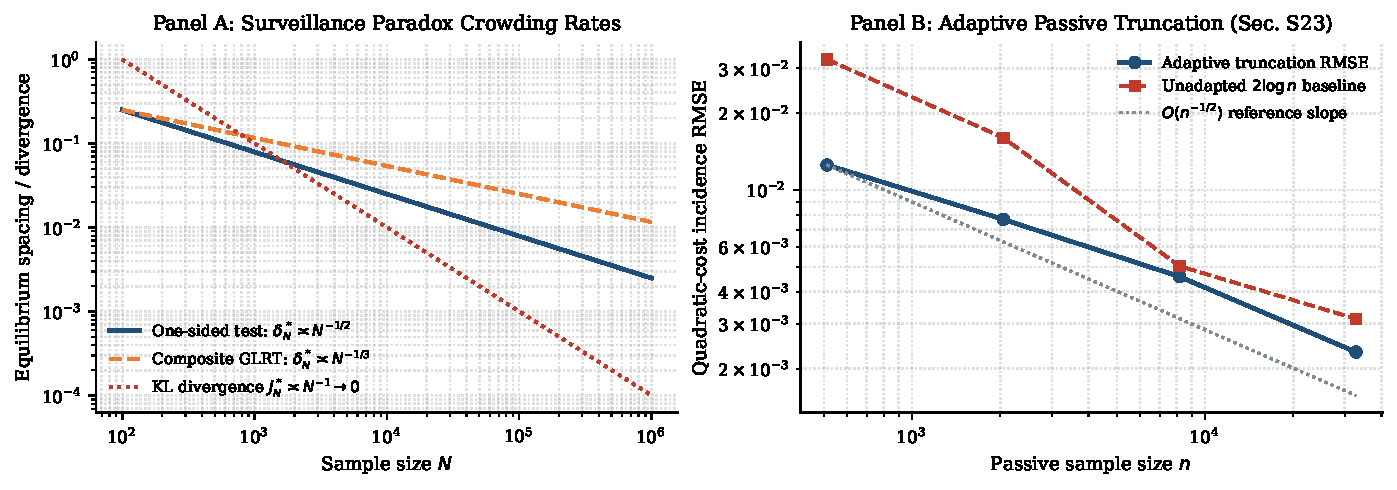
\includegraphics[width=.94\linewidth]{fig_supp_surveillance_mpv.pdf}
\caption{Surveillance paradox crowding rates under one-sided vs.\ composite GLRT tests (Panel~A, Proposition~\ref{prop:endogenous_supervisor}) and adaptive vs.\ unadapted passive-incidence RMSE across sample sizes (Panel~B).}\label{fig:supp_surveillance_mpv}\end{figure}


\section{Rational inattention, solvency boundaries, and noise deconvolution}\label{app:microfoundations}

\subsection{Microfounding exponential memory via subjective-AR(1) rational inattention}\label{sec:inattention}
In the public-$F_t$ inventory benchmark (Remark~\ref{M-rem:obs}), exponential memory rules represent boundedly rational or mandate-constrained execution schedules rather than frictionless full-information arbitrage (which would trade immediately against mean-reverting $x_t$). Formally, under dynamic LQG rational inattention \citep{sims2003,mackowiak2009}, desk $i$ tracks $x_t$ using a capacity-constrained subjective AR(1) / persistent-trend working model with per-bit information flow cost $\mu_i > 0$, yielding the steady-state Kalman recursion
\[
  \hat{x}_{i,t} = (1 - \eta_i^*) \hat{x}_{i,t-1} + \eta_i^* x_t + \tilde{\xi}_{i,t}, \qquad r_i = 1 - \eta_i^*(\mu_i) \in (0, 1).
\]
As analyzed in Section~\ref{sec:kyle_hostoll} and Remark~\ref{M-rem:returns}, idiosyncratic channel-processing noise $\tilde{\xi}_{i,t}$ enters aggregate customer order flow as an additive variance component while leaving the deterministic feedback kernel $k_m = \sum_i w_i r_i^m$ and closed-loop poles intact.

\subsection{Drawdown constraints and the domain of linear kernel sufficiency}\label{sec:solvency}
Under unbounded Gaussian innovations, strict zero-ruin probability $\mathbb{P}(\inf_t W_{i,t} \le 0) = 0$ is infeasible for any non-zero position rule. Realistic desks instead enforce mechanical state-dependent drawdown caps $|u_{i,t}| \le \bar{u}(W_{i,t})$ prior to risk-limit activation. Once wealth or position thresholds bind ($W_{i,t} \le \bar{W}_{\mathrm{crit}}$), individual order flow becomes a nonlinear path-dependent functional of group-specific wealth histories, breaking global linear kernel sufficiency (Theorem~\ref{M-n:suff}): two populations with identical linear kernels $k_m$ diverge pathwise as soon as a concentrated group hits its risk limit while split groups remain unconstrained. Theorem~\ref{M-n:suff} therefore governs the interior well-capitalized mechanical-rule regime strictly prior to the first stopping time $\tau_{\mathrm{bind}}$ (pre-binding behavioral anticipation of $\tau_{\mathrm{bind}}$ would alter trading rules beforehand and lies outside fixed-rule sufficiency).

\subsection{Minimum price variation and stochastic dithering details}\label{sec:mpv_supp}

\noindent This result was moved from the main text (Section~\ref{M-sec:cost}). Discrete exchange tick grids do not rescue compositional identification---and can extinguish it completely when shocks remain sub-tick:

\begin{theorem}[Minimum price variation and tick-grid resolution]\label{thm:mpv}
Let transaction prices $p_t = F_t + x_t$ be rounded onto a uniform tick grid $\Delta_{\mathrm{tick}} > 0$ via $\mathcal{Q}(p) = \Delta_{\mathrm{tick}} \lfloor p / \Delta_{\mathrm{tick}} + 1/2 \rfloor$ (under either open-loop observer rounding or closed-loop exchange tick clearing) for two $K$-group economies satisfying $\|h^A - h^B\|_1 \le C (\Delta\eta)^{2K-1}$ (or $\|k^A - k^B\|_1 \le C_k(\Delta\eta)^{2K-1}$ in closed loop).
\begin{enumerate}
  \item[(i)] \emph{Sub-cell coincidence.} Under bounded shocks $\|v\|_\infty \le \bar{v}$, if the baseline trajectory $p_t^A$ stays strictly farther than $C_{\mathrm{cl}}(\bar{v} + \|\tilde{x}^A\|_\infty)(\Delta\eta)^{2K-1}$ from every half-tick boundary $(m + \tfrac{1}{2})\Delta_{\mathrm{tick}}$, then $\mathcal{Q}(p_t^A) = \mathcal{Q}(p_t^B)$ pathwise, $\KL(P_{\mathcal{Q}}^A \| P_{\mathcal{Q}}^B) = 0$, and $N = \infty$; bounded continuous shocks crossing a half-tick boundary yield positive $\KL$.
  \item[(ii)] \emph{Gaussian dithering.} Under $N(0,\sigma^2)$ innovations, quantized Fisher information satisfies $\mathcal{I}_{\mathcal{Q}}(\mu) > 0$ for every $\Delta_{\mathrm{tick}} > 0$, and data processing preserves $\KL(P_{\mathcal{Q}}^A \| P_{\mathcal{Q}}^B) \le C T (\Delta\eta)^{4K-2}$. As $\Delta_{\mathrm{tick}}/\sigma \to 0$, independent reset impulses preserve the $(\Delta\eta)^{4K-2}$ lower bound with Sheppard efficiency $1 - \Delta_{\mathrm{tick}}^2/(12\sigma^2) + O(\Delta_{\mathrm{tick}}^4/\sigma^4)$, while passive $\mathrm{AR}(1)$ records incur double-quantization Whittle factor $1 - (1 - a^2)\Delta_{\mathrm{tick}}^2/(6\sigma^2) + O(\Delta_{\mathrm{tick}}^4/\sigma^4)$ alongside Markov-chain conditioning loss.
\end{enumerate}
\end{theorem}

\begin{proof}[Proof of Theorem~\ref{thm:mpv}]
For~(i), $|p_t^A - p_t^B| \le C_{\mathrm{cl}}(\bar{v} + \|\tilde{x}^A\|_\infty)(\Delta\eta)^{2K-1}$ whenever both trajectories remain inside the same tick cell through $t - 1$ (inductively, quantized state deviations vanish while $\tilde{x}_s^B = \tilde{x}_s^A$); hence $\max_t |p_t^A - m_t \Delta_{\mathrm{tick}}| + C_{\mathrm{cl}}(\bar{v} + \|\tilde{x}^A\|_\infty)(\Delta\eta)^{2K-1} < \Delta_{\mathrm{tick}}/2$ confines both $p_t^A$ and $p_t^B$ to $[(m_t-\tfrac{1}{2})\Delta_{\mathrm{tick}}, (m_t+\tfrac{1}{2})\Delta_{\mathrm{tick}})$ for all $t$, giving pathwise coincidence and $\KL = 0$. For~(ii), data processing gives $\KL(P_{\mathcal{Q}}^A \| P_{\mathcal{Q}}^B) \le \KL(P^A \| P^B)$; for every $\Delta_{\mathrm{tick}} > 0$, strictly positive Gaussian density renders each cell probability $C^2$-sensitive to mean shifts ($\mathcal{I}_{\mathcal{Q}} > 0$), preserving the $(\Delta\eta)^{4K-2}$ order on independent reset impulses with small-tick Sheppard limit $1 - \Delta_{\mathrm{tick}}^2/(12\sigma^2)$ and passive $\mathrm{AR}(1)$ double-quantization Whittle factor $1 - (1 - a^2)\Delta_{\mathrm{tick}}^2/(6\sigma^2)$.
\end{proof}

Under discrete rounding $\mathcal{Q}(p) = \Delta_{\mathrm{tick}} \lfloor p / \Delta_{\mathrm{tick}} + 1/2 \rfloor$, two regimes arise in Theorem~\ref{thm:mpv}. First, under bounded innovations $\|v\|_\infty \le \bar{v}$ whose baseline closed-loop trajectory satisfies $|p_t^A - m_t \Delta_{\mathrm{tick}}| + C_{\mathrm{cl}}(\bar{v} + \|\tilde{x}^A\|_\infty) (\Delta\eta)^{2K-1} < \Delta_{\mathrm{tick}}/2$ around integer tick indices $m_t$, $\mathcal{Q}(p_t^A) = \mathcal{Q}(p_t^B)$ identically (including closed-loop tick feedback; \nolinkurl{PublicationRevision16.lean}) and $\KL(P_{\mathcal{Q}}^A \| P_{\mathcal{Q}}^B) = 0$. Second, under continuous Gaussian innovations $\varepsilon_t \sim N(0, \sigma^2)$, noise crosses cell boundaries with positive probability (`stochastic dithering'): each tick cell $m$ has probability $p_m(\mu_t) = \Phi(((m+\tfrac{1}{2})\Delta_{\mathrm{tick}} - \mu_t)/\sigma) - \Phi(((m-\tfrac{1}{2})\Delta_{\mathrm{tick}} - \mu_t)/\sigma)$ with derivative $\partial_{\mu} p_m(\mu_t) = -\sigma^{-1}[\phi(((m+\tfrac{1}{2})\Delta_{\mathrm{tick}} - \mu_t)/\sigma) - \phi(((m-\tfrac{1}{2})\Delta_{\mathrm{tick}} - \mu_t)/\sigma)]$, so shifting the conditional mean by $\delta_t = O((\Delta\eta)^{2K-1})$ shifts cell probabilities by $\Delta p_m = (\partial_\mu p_m(\mu_t))\,\delta_t + O(\delta_t^2)$. For every $\Delta_{\mathrm{tick}} > 0$, quantized Fisher information $\mathcal{I}_{\mathcal{Q}}(\mu_t) = \sum_{m\in\mathbb{Z}} (\partial_\mu p_m)^2 / p_m$ is strictly positive (the $2\sqrt{3}\,\sigma$ zero of $1 - \Delta_{\mathrm{tick}}^2/(12\sigma^2)$ is solely a truncated small-tick expansion artifact as $\Delta_{\mathrm{tick}}/\sigma \to 0$); in stationary AR(1) records where both lagged and current prices are rounded (`HMM double quantization'), the small-tick Whittle Fisher efficiency for autoregressive persistence $a$ obeys $1 - (1 - a^2)\Delta_{\mathrm{tick}}^2/(6\sigma^2) + O(\Delta_{\mathrm{tick}}^4/\sigma^4)$ (generalizing via spectral curvature integration for higher-order feedback ARMA) alongside Markov-chain conditioning loss (\nolinkurl{PublicationRevision16.lean}).

\subsection{Discrete Roll-bounce deconvolution vs.\ infill pre-averaging}\label{sec:preaveraging}
When observed prices contain additive i.i.d.\ microstructure noise $\tilde{x}_t = x_t + \eta_t$ with $\E[\eta_t] = 0$, $\operatorname{Var}(\eta_t) = \sigma_\eta^2$ \citep{roll1984}, raw lag-zero sample autocovariances suffer $O(1)$ upward bias $+\sigma_\eta^2$, attenuating cepstral coefficients $\ell_j$ and inducing spurious feedback poles. In our discrete-time unit-step ARMA model, $\operatorname{Cov}(\eta_t, \eta_{t-m}) = 0$ for every lag $m \ge 1$, so higher-lag sample autocovariances $\hat{\gamma}_m(\tilde{x}) = \gamma_m(x) + O_P(n^{-1/2})$ ($m \ge 1$) remain unbiased. Crucially, naively subtracting an estimated noise variance $\hat\sigma_\eta^2$ at lag~$0$ without joint Toeplitz positive-semidefinite regularization can produce negative deconvolved spectra ($\tilde f^{\mathrm{deconv}}(\omega) \le 0$) and hit spectral floors, while unrestricted high-order shifted Yule--Walker Hankel systems become rank-deficient once $L > K+1$. Instead, parametric estimation fits a positive rational ARMA/spectral factor $f_x(\omega) = \sigma_x^2 / |Q(e^{-i\omega})|^2 \ge f_{\min} > 0$ directly to lags $m \ge 1$ (or via Toeplitz-PSD-constrained Whittle/covariance matching), guaranteeing PSD spectra and restoring the $O_P(n^{-1/2})$ parametric rate. Conversely, in the high-frequency infill Ornstein--Uhlenbeck limit ($\Delta_n \to 0$), adjacent signal increments shrink relative to bounce noise, requiring level pre-averaged realized kernels over blocks $k_n = \lceil c_w n^{1/2}\rceil$ with triangle weights $w_j = \min(u, 1-u)$ \citep{jacod2009,barndorff2008} and noise-bias subtraction across $0 \le m < k_n$, which yields the infill noise-limited rate $O_P(n^{-1/4})$.

\begin{thebibliography}{99}\setlength{\itemsep}{2pt}\small
\bibitem[Abramowitz and Stegun(1964)]{abramowitz1964} Abramowitz, M., and I. A. Stegun (1964). \emph{Handbook of Mathematical Functions}. National Bureau of Standards, Washington, DC.

\bibitem[Avellaneda and Stoikov(2008)]{avellaneda2008} Avellaneda, M., and S. Stoikov (2008). High-frequency trading in a limit order book. \emph{Quantitative Finance} 8, 217--224.

\bibitem[Barberis et~al.(2015)]{barberis2015} Barberis, N., R. Greenwood, L. Jin, and A. Shleifer (2015). X-CAPM: An extrapolative capital asset pricing model. \emph{Journal of Financial Economics} 115, 1--24.

\bibitem[Barberis et~al.(2018)]{barberis2018} Barberis, N., R. Greenwood, L. Jin, and A. Shleifer (2018). Extrapolation and bubbles. \emph{Journal of Financial Economics} 129, 203--227.

\bibitem[Barndorff-Nielsen et~al.(2008)]{barndorff2008} Barndorff-Nielsen, O.~E., P.~R. Hansen, A. Lunde, and N. Shephard (2008). Designing realized kernels to measure the ex post variation of equity prices in the presence of noise. \emph{Econometrica} 76(6), 1481--1536.

\bibitem[Border and Sobel(1987)]{border1987} Border, K.~C., and J. Sobel (1987). Samurai accountant: A theory of auditing and plunder. \emph{Review of Economic Studies} 54(4), 525--540.

\bibitem[Brillinger(1965)]{brillinger1965} Brillinger, D.~R. (1965). An introduction to polyspectra. \emph{Annals of Mathematical Statistics} 36(5), 1351--1374.

\bibitem[Brunnermeier and Pedersen(2009)]{brunnermeier2009} Brunnermeier, M.~K., and L.~H. Pedersen (2009). Market liquidity and funding liquidity. \emph{Review of Financial Studies} 22(6), 2201--2238.

\bibitem[Budish et~al.(2015)]{budish2015} Budish, E., P. Cramton, and J. Shim (2015). The high-frequency trading arms race: Frequent batch auctions as a market design response. \emph{Quarterly Journal of Economics} 130(4), 1547--1621.

\bibitem[Cagan(1956)]{cagan1956} Cagan, P. (1956). The monetary dynamics of hyperinflation. In M. Friedman (Ed.), \emph{Studies in the Quantity Theory of Money}, 25--117. University of Chicago Press.

\bibitem[Donoho(1994)]{donoho1994} Donoho, D.~L. (1994). Statistical estimation and optimal recovery. \emph{Annals of Statistics} 22, 238--270.

\bibitem[Epstein and Schotland(2008)]{epstein2008} Epstein, C.~L., and J. Schotland (2008). The bad truth about Laplace's transform. \emph{SIAM Review} 50(3), 504--520.

\bibitem[Gautschi(2004)]{gautschi2004} Gautschi, W. (2004). \emph{Orthogonal Polynomials: Computation and Approximation}. Oxford University Press, Oxford.

\bibitem[Hale and Townsend(2013)]{hale2013} Hale, N., and A. Townsend (2013). Fast and accurate computation of Gauss--Legendre and Gauss--Jacobi quadrature nodes and weights. \emph{SIAM Journal on Scientific Computing} 35, A652--A674.

\bibitem[Hinich(1982)]{hinich1982} Hinich, M.~J. (1982). Testing for Gaussianity and linearity of a stationary time series. \emph{Journal of Time Series Analysis} 3(3), 169--176.

\bibitem[Ho and Stoll(1981)]{ho1981} Ho, T., and H.~R. Stoll (1981). Optimal dealer pricing under transactions and return uncertainty. \emph{Journal of Financial Economics} 9(1), 47--73.

\bibitem[Huberman and Stanzl(2004)]{huberman2004} Huberman, G., and W. Stanzl (2004). Price manipulation and quasi-arbitrage. \emph{Econometrica} 72(4), 1247--1275.

\bibitem[Ing and Wei(2005)]{ingwei2005} Ing, C.-K., and C.-Z. Wei (2005). Order selection for same-realization predictions in autoregressive processes. \emph{Annals of Statistics} 33(5), 2423--2474. \href{https://doi.org/10.1214/009053605000000525}{doi:10.1214/009053605000000525}.

\bibitem[Jacod et~al.(2009)]{jacod2009} Jacod, J., Y. Li, P.~A. Mykland, M. Podolskij, and M. Vetter (2009). Microstructure noise in the continuous case: The pre-averaging approach. \emph{Stochastic Processes and their Applications} 119(7), 2249--2276.

\bibitem[Katz et~al.(2023)]{katz2023} Katz, R., N. Diab, and D. Batenkov (2023). On the accuracy of Prony's method for recovery of exponential sums with closely spaced exponents. arXiv preprint arXiv:2302.05883.

\bibitem[Koyck(1954)]{koyck1954} Koyck, L.~M. (1954). \emph{Distributed Lags and Investment Analysis}. North-Holland.

\bibitem[Kyle(1985)]{kyle1985} Kyle, A. S. (1985). Continuous auctions and insider trading. \emph{Econometrica} 53, 1315--1335.

\bibitem[Ma\'ckowiak and Wiederholt(2009)]{mackowiak2009} Ma\'ckowiak, B., and M. Wiederholt (2009). Optimal sticky prices under rational inattention. \emph{American Economic Review} 99(3), 769--807.

\bibitem[Mancini(2009)]{mancini2009} Mancini, C. (2009). Non-parametric threshold estimation for models with stochastic diffusion coefficient and jumps. \emph{Scandinavian Journal of Statistics} 36(2), 270--296.

\bibitem[Muth(1960)]{muth1960} Muth, J.~F. (1960). Optimal properties of exponentially weighted forecasts. \emph{Journal of the American Statistical Association} 55, 299--306.

\bibitem[Nerlove(1958)]{nerlove1958} Nerlove, M. (1958). Adaptive expectations and cobweb phenomena. \emph{Quarterly Journal of Economics} 72, 227--240.

\bibitem[Niroula et~al.(2026a)]{niroula2026a} Niroula, P., P. Niroula, and S. Khatiwada (2026a). What prices cannot tell a market supervisor: The cost of identifying trader groups and the value of class disclosure. Working paper, 5 November 2026, \url{https://github.com/Pratikn03/Fianince}.

\bibitem[Niroula et~al.(2026b)]{niroula2026b} Niroula, P., S. Alkhushayni, Y. Chen, M. Bhavsar, and P. Niroula (2026b). From human markets to machine markets: Transient amplification, an exact depth condition, and a maximal pre-trade guard. Working paper, Minnesota State University, Mankato.

\bibitem[Niroula et~al.(2026c)]{niroula2026c} Niroula, P., P. Niroula, and S. Khatiwada (2026c). After a breach, and beyond linear rules: Companion results to ``Observationally equivalent algorithms''. Working paper, 13 November 2026, \url{https://github.com/Pratikn03/Fianince}.

\bibitem[Niroula et~al.(2026d)]{niroula2026full} Niroula, P., P. Niroula, and S. Khatiwada (2026d). Observationally equivalent algorithms: Full working paper with all supplementary results. Working paper, 21 November 2026, \url{https://github.com/Pratikn03/Fianince}.

\bibitem[Roll(1984)]{roll1984} Roll, R. (1984). A simple implicit measure of the effective bid-ask spread in an efficient market. \emph{Journal of Finance} 39, 1127--1139.

\bibitem[Sims(2003)]{sims2003} Sims, C.~A. (2003). Implications of rational inattention. \emph{Journal of Monetary Economics} 50(3), 665--690.

\bibitem[Subrahmanyam(1994)]{subrahmanyam1994} Subrahmanyam, A. (1994). Circuit breakers and market volatility: A theoretical perspective. \emph{Journal of Finance} 49(1), 237--254.

\bibitem[Szeg\H{o}(1975)]{szego1975} Szeg\H{o}, G. (1975). \emph{Orthogonal Polynomials}, 4th ed. American Mathematical Society Colloquium Publications 23, Providence, RI.

\bibitem[Tsybakov(2009)]{tsybakov2009} Tsybakov, A. B. (2009). \emph{Introduction to Nonparametric Estimation}. Springer.

\bibitem[Wu and Wang(2020)]{wuwang2020} Wu, C.-H., and T.-Y. Wang (2020). The effects of reducing the securities transaction tax on day trading: Evidence from the Taiwan stock market. \emph{Journal of Accounting Review} 70, 135--169.
\end{thebibliography}
\end{document}
